\documentclass[a4paper,14pt,oneside,openany]{memoir}

%%%%%%%%%%%%%%%%%%%%%%%%%%%%%%%%%%%%%%%%%%%%%%%%%%%%%%%%%%%%%%%%%%%%%%%%%%%%%%%%
%%%% Файл упрощённых настроек шаблона, общих для диссертации и автореферата %%%%
%%%%%%%%%%%%%%%%%%%%%%%%%%%%%%%%%%%%%%%%%%%%%%%%%%%%%%%%%%%%%%%%%%%%%%%%%%%%%%%%

%%% Режим черновика %%%
\makeatletter
\@ifundefined{c@draft}{
  \newcounter{draft}
  \setcounter{draft}{0}  % 0 --- чистовик (максимальное соблюдение ГОСТ)
                         % 1 --- черновик (отклонения от ГОСТ, но быстрая
                         %       сборка итоговых PDF)
}{}
\makeatother

%%% Пометки в тексте %%%
\makeatletter
\@ifundefined{c@showmarkup}{
  \newcounter{showmarkup}
  \setcounter{showmarkup}{0}  % 0 --- скрыть пометки
                              % 1 --- показывать пометки
}{}
\makeatother

%%% Использование в pdflatex шрифтов не по-умолчанию %%%
\makeatletter
\@ifundefined{c@usealtfont}{
  \newcounter{usealtfont}
  \setcounter{usealtfont}{2}    % 0 --- шрифты на базе Computer Modern
                                % 1 --- использовать пакет pscyr, при его
                                %       наличии
                                % 2 --- использовать пакет XCharter, при наличии
                                %       подходящей версии
}{}
\makeatother

%%% Использование в xelatex и lualatex семейств шрифтов %%%
\makeatletter
\@ifundefined{c@fontfamily}{
  \newcounter{fontfamily}
  \setcounter{fontfamily}{2}  % 0 --- CMU семейство. Используется как fallback;
                              % 1 --- Шрифты от MS (Times New Roman и компания)
                              % 2 --- Семейство Liberation
}{}
\makeatother


%%% Вывод типов ссылок в библиографии %%%
\makeatletter
\@ifundefined{c@mediadisplay}{
  \newcounter{mediadisplay}
  \setcounter{mediadisplay}{1}   % 0 --- не делать ничего; надписи [Текст] и
                                 %       [Эл. ресурс] будут выводиться только в ссылках с
                                 %       заполненным полем `media`;
                                 % 1 --- автоматически добавлять надпись [Текст] к ссылкам с
                                 %       незаполненным полем `media`; таким образом, у всех
                                 %       источников будет указан тип, что соответствует
                                 %       требованиям ГОСТ
                                 % 2 --- автоматически удалять надписи [Текст], [Эл. Ресурс] и др.;
                                 %       не соответствует ГОСТ
                                 % 3 --- автоматически удалять надпись [Текст];
                                 %       не соответствует ГОСТ
                                 % 4 --- автоматически удалять надпись [Эл. Ресурс];
                                 %       не соответствует ГОСТ
}{}
\makeatother

%%% Предкомпиляция tikz рисунков для ускорения работы %%%
\makeatletter
\@ifundefined{c@imgprecompile}{
  \newcounter{imgprecompile}
  \setcounter{imgprecompile}{0}   % 0 --- без предкомпиляции;
                                  % 1 --- пользоваться предварительно
                                  %       скомпилированными pdf вместо генерации
                                  %       заново из tikz
}{}
\makeatother
            % Общие настройки шаблона
%%% Проверка используемого TeX-движка %%%
\newif\ifxetexorluatex   % определяем новый условный оператор (http://tex.stackexchange.com/a/47579)
\ifxetex
    \xetexorluatextrue
\else
    \ifluatex
        \xetexorluatextrue
    \else
        \xetexorluatexfalse
    \fi
\fi

\usepackage{etoolbox}[2015/08/02]   % Для продвинутой проверки разных условий
\providebool{presentation}

\usepackage{comment}    % Позволяет убирать блоки текста (добавляет
                        % окружение comment и команду \excludecomment)

%%% Поля и разметка страницы %%%
\usepackage{pdflscape}  % Для включения альбомных страниц
\usepackage{geometry}   % Для последующего задания полей

%%% Математические пакеты %%%
\usepackage{amsmath,amsthm}
% \usepackage{amscd}
\usepackage{amsfonts,amssymb}       % Математические дополнения от AMS
\usepackage{mathtools}              % Добавляет окружение multlined
\usepackage{thmtools}
\usepackage{xfrac}                  % Красивые дроби
\usepackage[
    locale = DE,
    list-separator       = {;\,},
    list-final-separator = {;\,},
    list-pair-separator  = {;\,},
    list-units           = single,
    range-units          = single,
    range-phrase={\text{\ensuremath{-}}},
    % quotient-mode        = fraction, % красивые дроби могут не соответствовать ГОСТ
    fraction-function    = \sfrac,
    separate-uncertainty,
    ]{siunitx}[=v2]                 % Размерности SI
\sisetup{inter-unit-product = \ensuremath{{}\cdot{}}}

% Кириллица в нумерации subequations
% Для правильной работы требуется выполнение сразу после загрузки пакетов
\patchcmd{\subequations}{\def\theequation{\theparentequation\alph{equation}}}
{\def\theequation{\theparentequation\asbuk{equation}}}
{\typeout{subequations patched}}{\typeout{subequations not patched}}

%%%% Установки для размера шрифта 14 pt %%%%
%% Формирование переменных и констант для сравнения (один раз для всех подключаемых файлов)%%
%% должно располагаться до вызова пакета fontspec или polyglossia, потому что они сбивают его работу
\newlength{\curtextsize}
\newlength{\bigtextsize}
\setlength{\bigtextsize}{13.9pt}

\makeatletter
%\show\f@size    % неплохо для отслеживания, но вызывает стопорение процесса,
                 % если документ компилируется без команды  -interaction=nonstopmode
\setlength{\curtextsize}{\f@size pt}
\makeatother

%%% Кодировки и шрифты %%%
\ifxetexorluatex
    \ifpresentation
        \providecommand*\autodot{} % quick fix for polyglossia 1.50
    \fi
    \PassOptionsToPackage{no-math}{fontspec}    % https://tex.stackexchange.com/a/26295/104425
    \usepackage{polyglossia}[2014/05/21]        % Поддержка многоязычности
                                        % (fontspec подгружается автоматически)
\else
   %%% Решение проблемы копирования текста в буфер кракозябрами
    \ifnumequal{\value{usealtfont}}{0}{}{
        \input glyphtounicode.tex
        \input glyphtounicode-cmr.tex %from pdfx package
        \pdfgentounicode=1
    }
    \usepackage{cmap}   % Улучшенный поиск русских слов в полученном pdf-файле
    \ifnumequal{\value{usealtfont}}{2}{}{
        \defaulthyphenchar=127  % Если стоит до fontenc, то переносы
                                % не впишутся в выделяемый текст при
                                % копировании его в буфер обмена
    }
    \usepackage{textcomp}
    \usepackage[T1,T2A]{fontenc}                    % Поддержка русских букв
    \ifnumequal{\value{usealtfont}}{1}{% Используется pscyr, при наличии
        \IfFileExists{pscyr.sty}{\usepackage{pscyr}}{}  % Подключение pscyr
    }{}
    \usepackage[utf8]{inputenc}[2014/04/30]         % Кодировка utf8
    \usepackage[english, russian]{babel}[2014/03/24]% Языки: русский, английский
    \makeatletter\AtBeginDocument{\let\@elt\relax}\makeatother % babel 3.40 fix
    \ifnumequal{\value{usealtfont}}{2}{
        % http://dxdy.ru/post1238763.html#p1238763
        \usepackage[scaled=0.914]{XCharter}[2017/12/19] % Подключение русифицированных шрифтов XCharter
        \usepackage[charter, vvarbb, scaled=1.048]{newtxmath}[2017/12/14]
        \ifpresentation
        \else
            \setDisplayskipStretch{-0.078}
        \fi
    }{}
\fi

%%% Оформление абзацев %%%
\ifpresentation
\else
    \indentafterchapter     % Красная строка после заголовков типа chapter
    \usepackage{indentfirst}
\fi

%%% Цвета %%%
\ifpresentation
\else
    \usepackage[dvipsnames, table, hyperref]{xcolor} % Совместимо с tikz
\fi

%%% Таблицы %%%
\usepackage{longtable,ltcaption} % Длинные таблицы
\usepackage{multirow,makecell}   % Улучшенное форматирование таблиц
\usepackage{tabu, tabulary}      % таблицы с автоматически подбирающейся
                                 % шириной столбцов (tabu обязательно
                                 % до hyperref вызывать)
\makeatletter
%https://github.com/tabu-issues-for-future-maintainer/tabu/issues/26
\@ifpackagelater{longtable}{2020/02/07}{
\def\tabuendlongtrial{%
    \LT@echunk  \global\setbox\LT@gbox \hbox{\unhbox\LT@gbox}\kern\wd\LT@gbox
                \LT@get@widths
}%
}{}
\makeatother

\usepackage{threeparttable} % автоматический подгон ширины подписи таблицы

%%% Общее форматирование
\usepackage{soul}    % Поддержка переносоустойчивых подчёркиваний и зачёркиваний
\usepackage{icomma}  % Запятая в десятичных дробях

%%% Оптимизация расстановки переносов и длины последней строки абзаца
\IfFileExists{impnattypo.sty}{% проверка установленности пакета impnattypo
    \ifluatex
        \ifnumequal{\value{draft}}{1}{% Черновик
            \usepackage[hyphenation, lastparline, nosingleletter, homeoarchy,
            rivers, draft]{impnattypo}
        }{% Чистовик
            \usepackage[hyphenation, lastparline, nosingleletter]{impnattypo}
        }
    \else
        \usepackage[hyphenation, lastparline]{impnattypo}
    \fi
}{}

%% Векторная графика

\usepackage{tikz}                   % Продвинутый пакет векторной графики
\usetikzlibrary{
    arrows.meta,
    calc,
    positioning,
}

%%% Гиперссылки %%%
\ifxetexorluatex
    \let\CYRDZE\relax
\fi
\usepackage{hyperref}[2012/11/06]

%%% Изображения %%%
\usepackage{graphicx}[2014/04/25]   % Подключаем пакет работы с графикой
\usepackage{caption}                % Подписи рисунков и таблиц
\usepackage{subcaption}             % Подписи подрисунков и подтаблиц
\usepackage{pdfpages}               % Добавление внешних pdf файлов

%%% Счётчики %%%
\usepackage{aliascnt}
\usepackage[figure,table]{totalcount}   % Счётчик рисунков и таблиц
\usepackage{totcount}   % Пакет создания счётчиков на основе последнего номера
                        % подсчитываемого элемента (может требовать дважды
                        % компилировать документ)
\usepackage{totpages}   % Счётчик страниц, совместимый с hyperref (ссылается
                        % на номер последней страницы). Желательно ставить
                        % последним пакетом в преамбуле

%%% Продвинутое управление групповыми ссылками (пока только формулами) %%%
\ifpresentation
\else
    \usepackage[russian]{cleveref} % cleveref имеет сложности со считыванием
    % языка из babel. Такое решение русификации вывода выбрано вместо
    % определения в documentclass из опасности что-то лишнее передать во все
    % остальные пакеты, включая библиографию.

    % Добавление возможности использования пробелов в \labelcref
    % https://tex.stackexchange.com/a/340502/104425
    \usepackage{kvsetkeys}
    \makeatletter
    \let\org@@cref\@cref
    \renewcommand*{\@cref}[2]{%
        \edef\process@me{%
            \noexpand\org@@cref{#1}{\zap@space#2 \@empty}%
        }\process@me
    }
    \makeatother
\fi

\usepackage{placeins} % для \FloatBarrier

\ifnumequal{\value{draft}}{1}{% Черновик
    \usepackage[firstpage]{draftwatermark}
    \SetWatermarkText{DRAFT}
    \SetWatermarkFontSize{14pt}
    \SetWatermarkScale{15}
    \SetWatermarkAngle{45}
}{}

%%% Цитата, не приводимая в автореферате:
% возможно, актуальна только для biblatex
%\newcommand{\citeinsynopsis}[1]{\ifsynopsis\else ~\cite{#1} \fi}

% если текущий процесс запущен библиотекой tikz-external, то прекомпиляция должна быть включена
\ifdefined\tikzexternalrealjob
    \setcounter{imgprecompile}{1}
\fi

\ifnumequal{\value{imgprecompile}}{1}{% Только если у нас включена предкомпиляция
    \usetikzlibrary{external}   % подключение возможности предкомпиляции
    \tikzexternalize[prefix=images/cache/,optimize command away=\includepdf] % activate! % здесь можно указать отдельную папку для скомпилированных файлов
    \ifxetex
        \tikzset{external/up to date check={diff}}
    \fi
}{}




%%% Прикладные пакеты %%%
%\usepackage{calc}               % Пакет для расчётов параметров, например длины

%%% Кавычки %%%
\usepackage{csquotes}

%%% Для добавления Стр. над номерами страниц в оглавлении
%%% http://tex.stackexchange.com/a/306950
\usepackage{afterpage}

%%% Списки %%%
\usepackage{enumitem}

%%% Оформление списка обозначений
\usepackage[intoc]{nomencl}
\makenomenclature
\setlength{\nomitemsep}{-.8\parsep}





\usepackage{fr-longtable}    %ради \endlasthead

% Листинги с исходным кодом программ
\usepackage{fancyvrb}
\usepackage{listings}
\lccode`\~=0\relax %Без этого хака из-за особенностей пакета listings перестают работать конструкции с \MakeLowercase и т. п. в (xe|lua)latex

% Русская традиция начертания греческих букв
\usepackage{upgreek} % прямые греческие ради русской традиции

%%% Микротипографика
%\ifnumequal{\value{draft}}{0}{% Только если у нас режим чистовика
	%    \usepackage[final, babel, shrink=45]{microtype}[2016/05/14] % улучшает представление букв и слов в строках, может помочь при наличии отдельно висящих слов
	%}{}

% Отметка о версии черновика на каждой странице
% Чтобы работало надо в своей локальной копии по инструкции
% https://www.ctan.org/pkg/gitinfo2 создать небходимые файлы в папке
% ./git/hooks
% If you’re familiar with tweaking git, you can probably work it out for
% yourself. If not, I suggest you follow these steps:
% 1. First, you need a git repository and working tree. For this example,
% let’s suppose that the root of the working tree is in ~/compsci
% 2. Copy the file post-xxx-sample.txt (which is in the same folder of
% your TEX distribution as this pdf) into the git hooks directory in your
% working copy. In our example case, you should end up with a file called
% ~/compsci/.git/hooks/post-checkout
% 3. If you’re using a unix-like system, don’t forget to make the file executable.
% Just how you do this is outside the scope of this manual, but one
% possible way is with commands such as this:
% chmod g+x post-checkout.
% 4. Test your setup with “git checkout master” (or another suitable branch
% name). This should generate copies of gitHeadInfo.gin in the directories
% you intended.
% 5. Now make two more copies of this file in the same directory (hooks),
% calling them post-commit and post-merge, and you’re done. As before,
% users of unix-like systems should ensure these files are marked as
% executable.
\ifnumequal{\value{draft}}{1}{% Черновик
	\IfFileExists{.git/gitHeadInfo.gin}{
		\usepackage[mark,pcount]{gitinfo2}
		\renewcommand{\gitMark}{rev.\gitAbbrevHash\quad\gitCommitterEmail\quad\gitAuthorIsoDate}
		\renewcommand{\gitMarkFormat}{\rmfamily\color{Gray}\small\bfseries}
	}{}
}{}

\usepackage{silence}
\WarningFilter[emptybib]{latex}{Empty bibliography}
\WarningFilter[keyword]{biblatex}{Keyword}
         % Пакеты, которые нужны для шаблона
%%%%%%%%%%%%%%%%%%%%%%%%%%%%%%%%%%%%%%%%%%%%%%%%%%%%%%
%%%% Файл упрощённых настроек шаблона диссертации %%%%
%%%%%%%%%%%%%%%%%%%%%%%%%%%%%%%%%%%%%%%%%%%%%%%%%%%%%%

%%% Инициализирование переменных, не трогать!  %%%
\newcounter{intvl}
\newcounter{otstup}
\newcounter{contnumeq}
\newcounter{contnumfig}
\newcounter{contnumtab}
\newcounter{pgnum}
\newcounter{chapstyle}
\newcounter{headingdelim}
\newcounter{headingalign}
\newcounter{headingsize}
%%%%%%%%%%%%%%%%%%%%%%%%%%%%%%%%%%%%%%%%%%%%%%%%%%%%%%

%%% Область упрощённого управления оформлением %%%

%% Интервал между заголовками и между заголовком и текстом %%
% Заголовки отделяют от текста сверху и снизу
% тремя интервалами (ГОСТ Р 7.0.11-2011, 5.3.5)
\setcounter{intvl}{1}               % Коэффициент кратности к размеру шрифта

%% Отступы у заголовков в тексте %%
\setcounter{otstup}{0}              % 0 --- без отступа; 1 --- абзацный отступ

%% Нумерация формул, таблиц и рисунков %%
% Нумерация формул
\setcounter{contnumeq}{1}   % 0 --- пораздельно (во введении подряд,
                            %       без номера раздела);
                            % 1 --- сквозная нумерация по всей диссертации
% Нумерация рисунков
\setcounter{contnumfig}{1}  % 0 --- пораздельно (во введении подряд,
                            %       без номера раздела);
                            % 1 --- сквозная нумерация по всей диссертации
% Нумерация таблиц
\setcounter{contnumtab}{1}  % 0 --- пораздельно (во введении подряд,
                            %       без номера раздела);
                            % 1 --- сквозная нумерация по всей диссертации

%% Оглавление %%
\setcounter{pgnum}{0}       % 0 --- номера страниц никак не обозначены;
                            % 1 --- Стр. над номерами страниц (дважды
                            %       компилировать после изменения настройки)
\settocdepth{subsection}    % до какого уровня подразделов выносить в оглавление
\setsecnumdepth{subsection} % до какого уровня нумеровать подразделы


%% Текст и форматирование заголовков %%
\setcounter{chapstyle}{1}     % 0 --- разделы только под номером;
                              % 1 --- разделы с названием "Глава" перед номером
\setcounter{headingdelim}{1}  % 0 --- номер отделен пропуском в 1em или \quad;
                              % 1 --- номера разделов и приложений отделены
                              %       точкой с пробелом, подразделы пропуском
                              %       без точки;
                              % 2 --- номера разделов, подразделов и приложений
                              %       отделены точкой с пробелом.

%% Выравнивание заголовков в тексте %%
\setcounter{headingalign}{0}  % 0 --- по центру;
                              % 1 --- по левому краю

%% Размеры заголовков в тексте %%
\setcounter{headingsize}{0}   % 0 --- по ГОСТ, все всегда 14 пт;
                              % 1 --- пропорционально изменяющийся размер
                              %       в зависимости от базового шрифта

%% Подпись таблиц %%

% Смещение строк подписи после первой строки
\newcommand{\tabindent}{0cm}

% Тип форматирования заголовка таблицы:
% plain --- название и текст в одной строке
% split --- название и текст в разных строках
\newcommand{\tabformat}{plain}

%%% Настройки форматирования таблицы `plain`

% Выравнивание по центру подписи, состоящей из одной строки:
% true  --- выравнивать
% false --- не выравнивать
\newcommand{\tabsinglecenter}{false}

% Выравнивание подписи таблиц:
% justified   --- выравнивать как обычный текст («по ширине»)
% centering   --- выравнивать по центру
% centerlast  --- выравнивать по центру только последнюю строку
% centerfirst --- выравнивать по центру только первую строку (не рекомендуется)
% raggedleft  --- выравнивать по правому краю
% raggedright --- выравнивать по левому краю
\newcommand{\tabjust}{justified}

% Разделитель записи «Таблица #» и названия таблицы
\newcommand{\tablabelsep}{~\cyrdash\ }

%%% Настройки форматирования таблицы `split`

% Положение названия таблицы:
% \centering   --- выравнивать по центру
% \raggedleft  --- выравнивать по правому краю
% \raggedright --- выравнивать по левому краю
\newcommand{\splitformatlabel}{\raggedleft}

% Положение текста подписи:
% \centering   --- выравнивать по центру
% \raggedleft  --- выравнивать по правому краю
% \raggedright --- выравнивать по левому краю
\newcommand{\splitformattext}{\raggedright}

%% Подпись рисунков %%
%Разделитель записи «Рисунок #» и названия рисунка
\newcommand{\figlabelsep}{~\cyrdash\ }  % (ГОСТ 2.105, 4.3.1)
                                        % "--- здесь не работает

%%% Цвета гиперссылок %%%
% Latex color definitions: http://latexcolor.com/
\definecolor{linkcolor}{rgb}{0.9,0,0}
\definecolor{citecolor}{rgb}{0,0.6,0}
\definecolor{urlcolor}{rgb}{0,0,1}
%\definecolor{linkcolor}{rgb}{0,0,0} %black
%\definecolor{citecolor}{rgb}{0,0,0} %black
%\definecolor{urlcolor}{rgb}{0,0,0} %black
      % Упрощённые настройки шаблона
%%% Кодировки и шрифты %%%
\ifxetexorluatex
    % Язык по-умолчанию русский с поддержкой приятных команд пакета babel
    \setmainlanguage[babelshorthands=true]{russian}
    % Дополнительный язык = английский (в американской вариации по-умолчанию)
    \setotherlanguage{english}

    % Проверка существования шрифтов. Недоступна в pdflatex
    \ifnumequal{\value{fontfamily}}{1}{
        \IfFontExistsTF{Times New Roman}{}{\setcounter{fontfamily}{0}}
    }{}
    \ifnumequal{\value{fontfamily}}{2}{
        \IfFontExistsTF{LiberationSerif}{}{\setcounter{fontfamily}{0}}
    }{}

    \ifnumequal{\value{fontfamily}}{0}{                    % Семейство шрифтов CMU. Используется как fallback
        \setmonofont{CMU Typewriter Text}                  % моноширинный шрифт
        \newfontfamily\cyrillicfonttt{CMU Typewriter Text} % моноширинный шрифт для кириллицы
        \defaultfontfeatures{Ligatures=TeX}                % стандартные лигатуры TeX, замены нескольких дефисов на тире и т. п. Настройки моноширинного шрифта должны идти до этой строки, чтобы при врезках кода программ в коде не применялись лигатуры и замены дефисов
        \setmainfont{CMU Serif}                            % Шрифт с засечками
        \newfontfamily\cyrillicfont{CMU Serif}             % Шрифт с засечками для кириллицы
        \setsansfont{CMU Sans Serif}                       % Шрифт без засечек
        \newfontfamily\cyrillicfontsf{CMU Sans Serif}      % Шрифт без засечек для кириллицы
    }

    \ifnumequal{\value{fontfamily}}{1}{                    % Семейство MS шрифтов
        \setmonofont{Courier New}                          % моноширинный шрифт
        \newfontfamily\cyrillicfonttt{Courier New}         % моноширинный шрифт для кириллицы
        \defaultfontfeatures{Ligatures=TeX}                % стандартные лигатуры TeX, замены нескольких дефисов на тире и т. п. Настройки моноширинного шрифта должны идти до этой строки, чтобы при врезках кода программ в коде не применялись лигатуры и замены дефисов
        \setmainfont{Times New Roman}                      % Шрифт с засечками
        \newfontfamily\cyrillicfont{Times New Roman}       % Шрифт с засечками для кириллицы
        \setsansfont{Arial}                                % Шрифт без засечек
        \newfontfamily\cyrillicfontsf{Arial}               % Шрифт без засечек для кириллицы
    }

    \ifnumequal{\value{fontfamily}}{2}{                    % Семейство шрифтов Liberation (https://pagure.io/liberation-fonts)
        \setmonofont{LiberationMono}[Scale=0.87] % моноширинный шрифт
        \newfontfamily\cyrillicfonttt{LiberationMono}[     % моноширинный шрифт для кириллицы
            Scale=0.87]
        \defaultfontfeatures{Ligatures=TeX}                % стандартные лигатуры TeX, замены нескольких дефисов на тире и т. п. Настройки моноширинного шрифта должны идти до этой строки, чтобы при врезках кода программ в коде не применялись лигатуры и замены дефисов
        \setmainfont{LiberationSerif}                      % Шрифт с засечками
        \newfontfamily\cyrillicfont{LiberationSerif}       % Шрифт с засечками для кириллицы
        \setsansfont{LiberationSans}                       % Шрифт без засечек
        \newfontfamily\cyrillicfontsf{LiberationSans}      % Шрифт без засечек для кириллицы
    }

\else
    \ifnumequal{\value{usealtfont}}{1}{% Используется pscyr, при наличии
        \IfFileExists{pscyr.sty}{\renewcommand{\rmdefault}{ftm}}{}
    }{}
\fi
            % Определение шрифтов (частичное)
%%% Шаблон %%%
\DeclareRobustCommand{\fixme}{\textcolor{red}}  % решаем проблему превращения
                                % названия цвета в результате \MakeUppercase,
                                % http://tex.stackexchange.com/a/187930,
                                % \DeclareRobustCommand protects \fixme
                                % from expanding inside \MakeUppercase
\AtBeginDocument{%
    \setlength{\parindent}{2.5em}                   % Абзацный отступ. Должен быть одинаковым по всему тексту и равен пяти знакам (ГОСТ Р 7.0.11-2011, 5.3.7).
}

%%% Таблицы %%%
\DeclareCaptionLabelSeparator{tabsep}{\tablabelsep} % нумерация таблиц
\DeclareCaptionFormat{split}{\splitformatlabel#1\par\splitformattext#3}

\captionsetup*[table]{
        format=\tabformat,                % формат подписи (plain|hang)
        font=normal,                      % нормальные размер, цвет, стиль шрифта
        skip=.0pt,                        % отбивка под подписью
        parskip=.0pt,                     % отбивка между параграфами подписи
        position=above,                   % положение подписи
        justification=\tabjust,           % центровка
        indent=\tabindent,                % смещение строк после первой
        labelsep=tabsep,                  % разделитель
        singlelinecheck=\tabsinglecenter, % не выравнивать по центру, если умещается в одну строку
}

%%% Рисунки %%%
\DeclareCaptionLabelSeparator{figsep}{\figlabelsep} % нумерация рисунков

\captionsetup*[figure]{
        format=plain,                     % формат подписи (plain|hang)
        font=normal,                      % нормальные размер, цвет, стиль шрифта
        skip=.0pt,                        % отбивка под подписью
        parskip=.0pt,                     % отбивка между параграфами подписи
        position=below,                   % положение подписи
        singlelinecheck=true,             % выравнивание по центру, если умещается в одну строку
        justification=centerlast,         % центровка
        labelsep=figsep,                  % разделитель
}

%%% Подписи подрисунков %%%
\DeclareCaptionSubType{figure}
\renewcommand\thesubfigure{\asbuk{subfigure}} % нумерация подрисунков
\DeclareCaptionFont{norm}{\fontsize{14pt}{16pt}\selectfont}
\newcommand{\subfigureskip}{0.pt}

\captionsetup*[subfloat]{
        labelfont=norm,                 % нормальный размер подписей подрисунков
        textfont=norm,                  % нормальный размер подписей подрисунков
        labelsep=space,                 % разделитель
        labelformat=brace,              % одна скобка справа от номера
        justification=centering,        % центровка
        singlelinecheck=true,           % выравнивание по центру, если умещается в одну строку
        skip=\subfigureskip,            % отбивка над подписью
        parskip=.0pt,                   % отбивка между параграфами подписи
        position=below,                 % положение подписи
}

%%% Настройки ссылок на рисунки, таблицы и др. %%%
% команды \cref...format отвечают за форматирование при помощи команды \cref
% команды \labelcref...format отвечают за форматирование при помощи команды \labelcref

\ifpresentation
\else
    \crefdefaultlabelformat{#2#1#3}

    % Уравнение
    \crefformat{equation}{(#2#1#3)} % одиночная ссылка с приставкой
    \labelcrefformat{equation}{(#2#1#3)} % одиночная ссылка без приставки
    \crefrangeformat{equation}{(#3#1#4) \cyrdash~(#5#2#6)} % диапазон ссылок с приставкой
    \labelcrefrangeformat{equation}{(#3#1#4) \cyrdash~(#5#2#6)} % диапазон ссылок без приставки
    \crefmultiformat{equation}{(#2#1#3)}{ и~(#2#1#3)}{, (#2#1#3)}{ и~(#2#1#3)} % перечисление ссылок с приставкой
    \labelcrefmultiformat{equation}{(#2#1#3)}{ и~(#2#1#3)}{, (#2#1#3)}{ и~(#2#1#3)} % перечисление без приставки

    % Подуравнение
    \crefformat{subequation}{(#2#1#3)} % одиночная ссылка с приставкой
    \labelcrefformat{subequation}{(#2#1#3)} % одиночная ссылка без приставки
    \crefrangeformat{subequation}{(#3#1#4) \cyrdash~(#5#2#6)} % диапазон ссылок с приставкой
    \labelcrefrangeformat{subequation}{(#3#1#4) \cyrdash~(#5#2#6)} % диапазон ссылок без приставки
    \crefmultiformat{subequation}{(#2#1#3)}{ и~(#2#1#3)}{, (#2#1#3)}{ и~(#2#1#3)} % перечисление ссылок с приставкой
    \labelcrefmultiformat{subequation}{(#2#1#3)}{ и~(#2#1#3)}{, (#2#1#3)}{ и~(#2#1#3)} % перечисление без приставки

    % Глава
    \crefformat{chapter}{#2#1#3} % одиночная ссылка с приставкой
    \labelcrefformat{chapter}{#2#1#3} % одиночная ссылка без приставки
    \crefrangeformat{chapter}{#3#1#4 \cyrdash~#5#2#6} % диапазон ссылок с приставкой
    \labelcrefrangeformat{chapter}{#3#1#4 \cyrdash~#5#2#6} % диапазон ссылок без приставки
    \crefmultiformat{chapter}{#2#1#3}{ и~#2#1#3}{, #2#1#3}{ и~#2#1#3} % перечисление ссылок с приставкой
    \labelcrefmultiformat{chapter}{#2#1#3}{ и~#2#1#3}{, #2#1#3}{ и~#2#1#3} % перечисление без приставки

    % Параграф
    \crefformat{section}{#2#1#3} % одиночная ссылка с приставкой
    \labelcrefformat{section}{#2#1#3} % одиночная ссылка без приставки
    \crefrangeformat{section}{#3#1#4 \cyrdash~#5#2#6} % диапазон ссылок с приставкой
    \labelcrefrangeformat{section}{#3#1#4 \cyrdash~#5#2#6} % диапазон ссылок без приставки
    \crefmultiformat{section}{#2#1#3}{ и~#2#1#3}{, #2#1#3}{ и~#2#1#3} % перечисление ссылок с приставкой
    \labelcrefmultiformat{section}{#2#1#3}{ и~#2#1#3}{, #2#1#3}{ и~#2#1#3} % перечисление без приставки

    % Приложение
    \crefformat{appendix}{#2#1#3} % одиночная ссылка с приставкой
    \labelcrefformat{appendix}{#2#1#3} % одиночная ссылка без приставки
    \crefrangeformat{appendix}{#3#1#4 \cyrdash~#5#2#6} % диапазон ссылок с приставкой
    \labelcrefrangeformat{appendix}{#3#1#4 \cyrdash~#5#2#6} % диапазон ссылок без приставки
    \crefmultiformat{appendix}{#2#1#3}{ и~#2#1#3}{, #2#1#3}{ и~#2#1#3} % перечисление ссылок с приставкой
    \labelcrefmultiformat{appendix}{#2#1#3}{ и~#2#1#3}{, #2#1#3}{ и~#2#1#3} % перечисление без приставки

    % Рисунок
    \crefformat{figure}{#2#1#3} % одиночная ссылка с приставкой
    \labelcrefformat{figure}{#2#1#3} % одиночная ссылка без приставки
    \crefrangeformat{figure}{#3#1#4 \cyrdash~#5#2#6} % диапазон ссылок с приставкой
    \labelcrefrangeformat{figure}{#3#1#4 \cyrdash~#5#2#6} % диапазон ссылок без приставки
    \crefmultiformat{figure}{#2#1#3}{ и~#2#1#3}{, #2#1#3}{ и~#2#1#3} % перечисление ссылок с приставкой
    \labelcrefmultiformat{figure}{#2#1#3}{ и~#2#1#3}{, #2#1#3}{ и~#2#1#3} % перечисление без приставки

    % Таблица
    \crefformat{table}{#2#1#3} % одиночная ссылка с приставкой
    \labelcrefformat{table}{#2#1#3} % одиночная ссылка без приставки
    \crefrangeformat{table}{#3#1#4 \cyrdash~#5#2#6} % диапазон ссылок с приставкой
    \labelcrefrangeformat{table}{#3#1#4 \cyrdash~#5#2#6} % диапазон ссылок без приставки
    \crefmultiformat{table}{#2#1#3}{ и~#2#1#3}{, #2#1#3}{ и~#2#1#3} % перечисление ссылок с приставкой
    \labelcrefmultiformat{table}{#2#1#3}{ и~#2#1#3}{, #2#1#3}{ и~#2#1#3} % перечисление без приставки

    % Листинг
    \crefformat{lstlisting}{#2#1#3} % одиночная ссылка с приставкой
    \labelcrefformat{lstlisting}{#2#1#3} % одиночная ссылка без приставки
    \crefrangeformat{lstlisting}{#3#1#4 \cyrdash~#5#2#6} % диапазон ссылок с приставкой
    \labelcrefrangeformat{lstlisting}{#3#1#4 \cyrdash~#5#2#6} % диапазон ссылок без приставки
    \crefmultiformat{lstlisting}{#2#1#3}{ и~#2#1#3}{, #2#1#3}{ и~#2#1#3} % перечисление ссылок с приставкой
    \labelcrefmultiformat{lstlisting}{#2#1#3}{ и~#2#1#3}{, #2#1#3}{ и~#2#1#3} % перечисление без приставки

    % Листинг
    \crefformat{ListingEnv}{#2#1#3} % одиночная ссылка с приставкой
    \labelcrefformat{ListingEnv}{#2#1#3} % одиночная ссылка без приставки
    \crefrangeformat{ListingEnv}{#3#1#4 \cyrdash~#5#2#6} % диапазон ссылок с приставкой
    \labelcrefrangeformat{ListingEnv}{#3#1#4 \cyrdash~#5#2#6} % диапазон ссылок без приставки
    \crefmultiformat{ListingEnv}{#2#1#3}{ и~#2#1#3}{, #2#1#3}{ и~#2#1#3} % перечисление ссылок с приставкой
    \labelcrefmultiformat{ListingEnv}{#2#1#3}{ и~#2#1#3}{, #2#1#3}{ и~#2#1#3} % перечисление без приставки
\fi

%%% Настройки гиперссылок %%%
\ifluatex
    \hypersetup{
        unicode,                % Unicode encoded PDF strings
    }
\fi

\hypersetup{
    linktocpage=true,       % ссылки с номера страницы в оглавлении, списке таблиц и списке рисунков
    linktoc=all,            % both the section and page part are links
    pdfpagelabels=false,    % set PDF page labels (true|false)
    plainpages=false,       % Forces page anchors to be named by the Arabic form  of the page number, rather than the formatted form
    colorlinks,             % ссылки отображаются раскрашенным текстом, а не раскрашенным прямоугольником, вокруг текста
    linkcolor={linkcolor},  % цвет ссылок типа ref, eqref и подобных
    citecolor={citecolor},  % цвет ссылок-цитат
    urlcolor={urlcolor},    % цвет гиперссылок
    hidelinks,              % Hide links (removing color and border)
    pdftitle={PhD Thesis},             % Заголовок
    pdfauthor={Konstantin Chukharev},  % Автор
    pdfsubject={2.3.5 Software},       % Тема
	% pdfcreator={Создатель},            % Создатель, Приложение
    % pdfproducer={Производитель},       % Производитель, Производитель PDF
    pdfkeywords={computer science},    % Ключевые слова
    pdflang={ru},
}
\ifnumequal{\value{draft}}{1}{% Черновик
    \hypersetup{
        draft,
    }
}{}

%%% Списки %%%
% Используем короткое тире (endash) для ненумерованных списков (ГОСТ 2.105-95, пункт 4.1.7, требует дефиса, но так лучше смотрится)
\renewcommand{\labelitemi}{\normalfont\bfseries{--}}

% Перечисление строчными буквами латинского алфавита (ГОСТ 2.105-95, 4.1.7)
%\renewcommand{\theenumi}{\alph{enumi}}
%\renewcommand{\labelenumi}{\theenumi)}

% Перечисление строчными буквами русского алфавита (ГОСТ 2.105-95, 4.1.7)
\makeatletter
\AddEnumerateCounter{\asbuk}{\russian@alph}{щ}      % Управляем списками/перечислениями через пакет enumitem, а он 'не знает' про asbuk, потому 'учим' его
\makeatother
%\renewcommand{\theenumi}{\asbuk{enumi}} %первый уровень нумерации
%\renewcommand{\labelenumi}{\theenumi)} %первый уровень нумерации
\renewcommand{\theenumii}{\asbuk{enumii}} %второй уровень нумерации
\renewcommand{\labelenumii}{\theenumii)} %второй уровень нумерации
\renewcommand{\theenumiii}{\arabic{enumiii}} %третий уровень нумерации
\renewcommand{\labelenumiii}{\theenumiii)} %третий уровень нумерации

\setlist{nosep,%                                    % Единый стиль для всех списков (пакет enumitem), без дополнительных интервалов.
    labelindent=\parindent,leftmargin=*%            % Каждый пункт, подпункт и перечисление записывают с абзацного отступа (ГОСТ 2.105-95, 4.1.8)
}

%%% Правильная нумерация приложений, рисунков и формул %%%
%% По ГОСТ 2.105, п. 4.3.8 Приложения обозначают заглавными буквами русского алфавита,
%% начиная с А, за исключением букв Ё, З, Й, О, Ч, Ь, Ы, Ъ.
%% Здесь также переделаны все нумерации русскими буквами.
\ifxetexorluatex
    \makeatletter
    \def\russian@Alph#1{\ifcase#1\or
       А\or Б\or В\or Г\or Д\or Е\or Ж\or
       И\or К\or Л\or М\or Н\or
       П\or Р\or С\or Т\or У\or Ф\or Х\or
       Ц\or Ш\or Щ\or Э\or Ю\or Я\else\xpg@ill@value{#1}{russian@Alph}\fi}
    \def\russian@alph#1{\ifcase#1\or
       а\or б\or в\or г\or д\or е\or ж\or
       и\or к\or л\or м\or н\or
       п\or р\or с\or т\or у\or ф\or х\or
       ц\or ш\or щ\or э\or ю\or я\else\xpg@ill@value{#1}{russian@alph}\fi}
    \def\cyr@Alph#1{\ifcase#1\or
        А\or Б\or В\or Г\or Д\or Е\or Ж\or
        И\or К\or Л\or М\or Н\or
        П\or Р\or С\or Т\or У\or Ф\or Х\or
        Ц\or Ш\or Щ\or Э\or Ю\or Я\else\xpg@ill@value{#1}{cyr@Alph}\fi}
    \def\cyr@alph#1{\ifcase#1\or
        а\or б\or в\or г\or д\or е\or ж\or
        и\or к\or л\or м\or н\or
        п\or р\or с\or т\or у\or ф\or х\or
        ц\or ш\or щ\or э\or ю\or я\else\xpg@ill@value{#1}{cyr@alph}\fi}
    \makeatother
\else
    \makeatletter
    \if@uni@ode
      \def\russian@Alph#1{\ifcase#1\or
        А\or Б\or В\or Г\or Д\or Е\or Ж\or
        И\or К\or Л\or М\or Н\or
        П\or Р\or С\or Т\or У\or Ф\or Х\or
        Ц\or Ш\or Щ\or Э\or Ю\or Я\else\@ctrerr\fi}
    \else
      \def\russian@Alph#1{\ifcase#1\or
        \CYRA\or\CYRB\or\CYRV\or\CYRG\or\CYRD\or\CYRE\or\CYRZH\or
        \CYRI\or\CYRK\or\CYRL\or\CYRM\or\CYRN\or
        \CYRP\or\CYRR\or\CYRS\or\CYRT\or\CYRU\or\CYRF\or\CYRH\or
        \CYRC\or\CYRSH\or\CYRSHCH\or\CYREREV\or\CYRYU\or
        \CYRYA\else\@ctrerr\fi}
    \fi
    \if@uni@ode
      \def\russian@alph#1{\ifcase#1\or
        а\or б\or в\or г\or д\or е\or ж\or
        и\or к\or л\or м\or н\or
        п\or р\or с\or т\or у\or ф\or х\or
        ц\or ш\or щ\or э\or ю\or я\else\@ctrerr\fi}
    \else
      \def\russian@alph#1{\ifcase#1\or
        \cyra\or\cyrb\or\cyrv\or\cyrg\or\cyrd\or\cyre\or\cyrzh\or
        \cyri\or\cyrk\or\cyrl\or\cyrm\or\cyrn\or
        \cyrp\or\cyrr\or\cyrs\or\cyrt\or\cyru\or\cyrf\or\cyrh\or
        \cyrc\or\cyrsh\or\cyrshch\or\cyrerev\or\cyryu\or
        \cyrya\else\@ctrerr\fi}
    \fi
    \makeatother
\fi


%%http://www.linux.org.ru/forum/general/6993203#comment-6994589 (используется totcount)
\makeatletter
\def\formtotal#1#2#3#4#5{%
    \newcount\@c
    \@c\totvalue{#1}\relax
    \newcount\@last
    \newcount\@pnul
    \@last\@c\relax
    \divide\@last 10
    \@pnul\@last\relax
    \divide\@pnul 10
    \multiply\@pnul-10
    \advance\@pnul\@last
    \multiply\@last-10
    \advance\@last\@c
    #2%
    \ifnum\@pnul=1#5\else%
    \ifcase\@last#5\or#3\or#4\or#4\or#4\else#5\fi
    \fi
}
\makeatother

\newcommand{\formbytotal}[5]{\total{#1}~\formtotal{#1}{#2}{#3}{#4}{#5}}

%%% Команды рецензирования %%%
\ifboolexpr{ (test {\ifnumequal{\value{draft}}{1}}) or (test {\ifnumequal{\value{showmarkup}}{1}})}{
        \newrobustcmd{\todo}[1]{\textcolor{red}{#1}}
        \newrobustcmd{\note}[2][]{\ifstrempty{#1}{#2}{\textcolor{#1}{#2}}}
        \newenvironment{commentbox}[1][]%
        {\ifstrempty{#1}{}{\color{#1}}}%
        {}
}{
        \newrobustcmd{\todo}[1]{}
        \newrobustcmd{\note}[2][]{}
        \excludecomment{commentbox}
}



%%% Переопределение именований, если иначе не сработает %%%
%\gappto\captionsrussian{
	%    \renewcommand{\chaptername}{Глава}
	%    \renewcommand{\appendixname}{Приложение} % (ГОСТ Р 7.0.11-2011, 5.7)
	%}

%%% Изображения %%%
\graphicspath{{images/}{Dissertation/images/}}         % Пути к изображениям

%%% Интервалы %%%
%% По ГОСТ Р 7.0.11-2011, пункту 5.3.6 требуется полуторный интервал
%% Реализация средствами класса (на основе setspace) ближе к типографской классике.
%% И правит сразу и в таблицах (если со звёздочкой)
%\DoubleSpacing*     % Двойной интервал
\OnehalfSpacing*    % Полуторный интервал
%\setSpacing{1.42}   % Полуторный интервал, подобный Ворду (возможно, стоит включать вместе с предыдущей строкой)

%%% Макет страницы %%%
% Выставляем значения полей (ГОСТ 7.0.11-2011, 5.3.7)
\geometry{a4paper, top=2cm, bottom=2cm, left=2.5cm, right=1cm, nofoot, nomarginpar} %, heightrounded, showframe
\setlength{\topskip}{0pt}   %размер дополнительного верхнего поля
\setlength{\footskip}{12.3pt} % снимет warning, согласно https://tex.stackexchange.com/a/334346

%%% Выравнивание и переносы %%%
%% http://tex.stackexchange.com/questions/241343/what-is-the-meaning-of-fussy-sloppy-emergencystretch-tolerance-hbadness
%% http://www.latex-community.org/forum/viewtopic.php?p=70342#p70342
\tolerance 1414
\hbadness 1414
\emergencystretch 2em % В случае проблем регулировать в первую очередь
\hfuzz 0.3pt
\vfuzz \hfuzz
% \raggedbottom
%\sloppy                 % Избавляемся от переполнений
\clubpenalty=10000      % Запрещаем разрыв страницы после первой строки абзаца
\widowpenalty=10000     % Запрещаем разрыв страницы после последней строки абзаца
\brokenpenalty=4991     % Ограничение на разрыв страницы, если строка заканчивается переносом

%%% Блок управления параметрами для выравнивания заголовков в тексте %%%
\newlength{\otstuplen}
\setlength{\otstuplen}{\theotstup\parindent}
\ifnumequal{\value{headingalign}}{0}{% выравнивание заголовков в тексте
	\newcommand{\hdngalign}{\centering}                % по центру
	\newcommand{\hdngaligni}{}% по центру
	\setlength{\otstuplen}{0pt}
}{%
	\newcommand{\hdngalign}{}                 % по левому краю
	\newcommand{\hdngaligni}{\hspace{\otstuplen}}      % по левому краю
} % В обоих случаях вроде бы без переноса, как и надо (ГОСТ Р 7.0.11-2011, 5.3.5)

%%% Оглавление %%%
\renewcommand{\cftchapterdotsep}{\cftdotsep}                % отбивка точками до номера страницы начала главы/раздела

%% Переносить слова в заголовке не допускается (ГОСТ Р 7.0.11-2011, 5.3.5). Заголовки в оглавлении должны точно повторять заголовки в тексте (ГОСТ Р 7.0.11-2011, 5.2.3). Прямого указания на запрет переносов в оглавлении нет, но по той же логике невнесения искажений в смысл, лучше в оглавлении не переносить:
\setrmarg{2.55em plus1fil}                             %To have the (sectional) titles in the ToC, etc., typeset ragged right with no hyphenation
\renewcommand{\cftchapterpagefont}{\normalfont}        % нежирные номера страниц у глав в оглавлении
\renewcommand{\cftchapterleader}{\cftdotfill{\cftchapterdotsep}}% нежирные точки до номеров страниц у глав в оглавлении
%\renewcommand{\cftchapterfont}{}                       % нежирные названия глав в оглавлении

\ifnumgreater{\value{headingdelim}}{0}{%
	\renewcommand\cftchapteraftersnum{.\space}       % добавляет точку с пробелом после номера раздела в оглавлении
}{}
\ifnumgreater{\value{headingdelim}}{1}{%
	\renewcommand\cftsectionaftersnum{.\space}       % добавляет точку с пробелом после номера подраздела в оглавлении
	\renewcommand\cftsubsectionaftersnum{.\space}    % добавляет точку с пробелом после номера подподраздела в оглавлении
	\renewcommand\cftsubsubsectionaftersnum{.\space} % добавляет точку с пробелом после номера подподподраздела в оглавлении
	\AfterEndPreamble{% без этого polyglossia сама всё переопределяет
		\setsecnumformat{\csname the#1\endcsname.\space}
	}
}{%
	\AfterEndPreamble{% без этого polyglossia сама всё переопределяет
		\setsecnumformat{\csname the#1\endcsname\quad}
	}
}

\renewcommand*{\cftappendixname}{\appendixname\space} % Слово Приложение в оглавлении

%%% Колонтитулы %%%
% Порядковый номер страницы печатают на середине верхнего поля страницы (ГОСТ Р 7.0.11-2011, 5.3.8)
\makeevenhead{plain}{}{\rmfamily\thepage}{}
\makeoddhead{plain}{}{\rmfamily\thepage}{}
\makeevenfoot{plain}{}{}{}
\makeoddfoot{plain}{}{}{}
\pagestyle{plain}

%%% добавить Стр. над номерами страниц в оглавлении
%%% http://tex.stackexchange.com/a/306950
\newif\ifendTOC

\newcommand*{\tocheader}{
	\ifnumequal{\value{pgnum}}{1}{%
		\ifendTOC\else\hbox to \linewidth%
		{\noindent{}~\hfill{Стр.}}\par%
		\ifnumless{\value{page}}{3}{}{%
			\vspace{0.5\onelineskip}
		}
		\afterpage{\tocheader}
		\fi%
	}{}%
}%

%%% Оформление заголовков глав, разделов, подразделов %%%
%% Работа должна быть выполнена ... размером шрифта 12-14 пунктов (ГОСТ Р 7.0.11-2011, 5.3.8). То есть не должно быть надписей шрифтом более 14. Так и поставим.
%% Эти установки будут давать одинаковый результат независимо от выбора базовым шрифтом 12 пт или 14 пт
\newcommand{\basegostsectionfont}{\fontsize{14pt}{16pt}\selectfont\bfseries}

\makechapterstyle{thesisgost}{%
	\chapterstyle{default}
	\setlength{\beforechapskip}{0pt}
	\setlength{\midchapskip}{0pt}
	\setlength{\afterchapskip}{\theintvl\curtextsize}
	\renewcommand*{\chapnamefont}{\basegostsectionfont}
	\renewcommand*{\chapnumfont}{\basegostsectionfont}
	\renewcommand*{\chaptitlefont}{\basegostsectionfont}
	\renewcommand*{\chapterheadstart}{}
	\ifnumgreater{\value{headingdelim}}{0}{%
		\renewcommand*{\afterchapternum}{.\space}   % добавляет точку с пробелом после номера раздела
	}{%
		\renewcommand*{\afterchapternum}{\quad}     % добавляет \quad после номера раздела
	}
	\renewcommand*{\printchapternum}{\hdngaligni\hdngalign\chapnumfont \thechapter}
	\renewcommand*{\printchaptername}{}
	\renewcommand*{\printchapternonum}{\hdngaligni\hdngalign}
}

\makeatletter
\makechapterstyle{thesisgostchapname}{%
	\chapterstyle{thesisgost}
	\renewcommand*{\printchapternum}{\chapnumfont \thechapter}
	\renewcommand*{\printchaptername}{\hdngaligni\hdngalign\chapnamefont \@chapapp} %
}
\makeatother

\chapterstyle{thesisgost}

\setsecheadstyle{\basegostsectionfont\hdngalign}
\setsecindent{\otstuplen}

\setsubsecheadstyle{\basegostsectionfont\hdngalign}
\setsubsecindent{\otstuplen}

\setsubsubsecheadstyle{\basegostsectionfont\hdngalign}
\setsubsubsecindent{\otstuplen}

\sethangfrom{\noindent #1} %все заголовки подразделов центрируются с учетом номера, как block

\ifnumequal{\value{chapstyle}}{1}{%
	\chapterstyle{thesisgostchapname}
	\renewcommand*{\cftchaptername}{\chaptername\space} % будет вписано слово Глава перед каждым номером раздела в оглавлении
}{}%

%%% Интервалы между заголовками
\setbeforesecskip{\theintvl\curtextsize}% Заголовки отделяют от текста сверху и снизу тремя интервалами (ГОСТ Р 7.0.11-2011, 5.3.5).
\setaftersecskip{\theintvl\curtextsize}
\setbeforesubsecskip{\theintvl\curtextsize}
\setaftersubsecskip{\theintvl\curtextsize}
\setbeforesubsubsecskip{\theintvl\curtextsize}
\setaftersubsubsecskip{\theintvl\curtextsize}

%%% Вертикальные интервалы глав (\chapter) в оглавлении как и у заголовков
% раскомментировать следующие 2
% \setlength{\cftbeforechapterskip}{0pt plus 0pt}   % ИЛИ эти 2 строки из учебника
% \renewcommand*{\insertchapterspace}{}
% или эту
% \renewcommand*{\cftbeforechapterskip}{0em}


%%% Блок дополнительного управления размерами заголовков
\ifnumequal{\value{headingsize}}{1}{% Пропорциональные заголовки и базовый шрифт 14 пт
	\renewcommand{\basegostsectionfont}{\large\bfseries}
	\renewcommand*{\chapnamefont}{\Large\bfseries}
	\renewcommand*{\chapnumfont}{\Large\bfseries}
	\renewcommand*{\chaptitlefont}{\Large\bfseries}
}{}

%%% Счётчики %%%

%% Упрощённые настройки шаблона диссертации: нумерация формул, таблиц, рисунков
\ifnumequal{\value{contnumeq}}{1}{%
	\counterwithout{equation}{chapter} % Убираем связанность номера формулы с номером главы/раздела
}{}
\ifnumequal{\value{contnumfig}}{1}{%
	\counterwithout{figure}{chapter}   % Убираем связанность номера рисунка с номером главы/раздела
}{}
\ifnumequal{\value{contnumtab}}{1}{%
	\counterwithout{table}{chapter}    % Убираем связанность номера таблицы с номером главы/раздела
}{}

\AfterEndPreamble{
	%% регистрируем счётчики в системе totcounter
	\regtotcounter{totalcount@figure}
	\regtotcounter{totalcount@table}       % Если иным способом поставить в преамбуле то ошибка в числе таблиц
	\regtotcounter{TotPages}               % Если иным способом поставить в преамбуле то ошибка в числе страниц
	\newtotcounter{totalappendix}
	\newtotcounter{totalchapter}
}


% для вертикального центрирования ячеек в tabulary
\def\zz{\ifx\[$\else\aftergroup\zzz\fi}
%$ \] % <-- чиним подсветку синтаксиса в некоторых редакторах
\def\zzz{\setbox0\lastbox
	\dimen0\dimexpr\extrarowheight + \ht0-\dp0\relax
	\setbox0\hbox{\raise-.5\dimen0\box0}%
	\ht0=\dimexpr\ht0+\extrarowheight\relax
	\dp0=\dimexpr\dp0+\extrarowheight\relax
	\box0
}

\lstdefinelanguage{Renhanced}%
{keywords={abbreviate,abline,abs,acos,acosh,action,add1,add,%
		aggregate,alias,Alias,alist,all,anova,any,aov,aperm,append,apply,%
		approx,approxfun,apropos,Arg,args,array,arrows,as,asin,asinh,%
		atan,atan2,atanh,attach,attr,attributes,autoload,autoloader,ave,%
		axis,backsolve,barplot,basename,besselI,besselJ,besselK,besselY,%
		beta,binomial,body,box,boxplot,break,browser,bug,builtins,bxp,by,%
		c,C,call,Call,case,cat,category,cbind,ceiling,character,char,%
		charmatch,check,chol,chol2inv,choose,chull,class,close,cm,codes,%
		coef,coefficients,co,col,colnames,colors,colours,commandArgs,%
		comment,complete,complex,conflicts,Conj,contents,contour,%
		contrasts,contr,control,helmert,contrib,convolve,cooks,coords,%
		distance,coplot,cor,cos,cosh,count,fields,cov,covratio,wt,CRAN,%
		create,crossprod,cummax,cummin,cumprod,cumsum,curve,cut,cycle,D,%
		data,dataentry,date,dbeta,dbinom,dcauchy,dchisq,de,debug,%
		debugger,Defunct,default,delay,delete,deltat,demo,de,density,%
		deparse,dependencies,Deprecated,deriv,description,detach,%
		dev2bitmap,dev,cur,deviance,off,prev,,dexp,df,dfbetas,dffits,%
		dgamma,dgeom,dget,dhyper,diag,diff,digamma,dim,dimnames,dir,%
		dirname,dlnorm,dlogis,dnbinom,dnchisq,dnorm,do,dotplot,double,%
		download,dpois,dput,drop,drop1,dsignrank,dt,dummy,dump,dunif,%
		duplicated,dweibull,dwilcox,dyn,edit,eff,effects,eigen,else,%
		emacs,end,environment,env,erase,eval,equal,evalq,example,exists,%
		exit,exp,expand,expression,External,extract,extractAIC,factor,%
		fail,family,fft,file,filled,find,fitted,fivenum,fix,floor,for,%
		For,formals,format,formatC,formula,Fortran,forwardsolve,frame,%
		frequency,ftable,ftable2table,function,gamma,Gamma,gammaCody,%
		gaussian,gc,gcinfo,gctorture,get,getenv,geterrmessage,getOption,%
		getwd,gl,glm,globalenv,gnome,GNOME,graphics,gray,grep,grey,grid,%
		gsub,hasTsp,hat,heat,help,hist,home,hsv,httpclient,I,identify,if,%
		ifelse,Im,image,\%in\%,index,influence,measures,inherits,install,%
		installed,integer,interaction,interactive,Internal,intersect,%
		inverse,invisible,IQR,is,jitter,kappa,kronecker,labels,lapply,%
		layout,lbeta,lchoose,lcm,legend,length,levels,lgamma,library,%
		licence,license,lines,list,lm,load,local,locator,log,log10,log1p,%
		log2,logical,loglin,lower,lowess,ls,lsfit,lsf,ls,machine,Machine,%
		mad,mahalanobis,make,link,margin,match,Math,matlines,mat,matplot,%
		matpoints,matrix,max,mean,median,memory,menu,merge,methods,min,%
		missing,Mod,mode,model,response,mosaicplot,mtext,mvfft,na,nan,%
		names,omit,nargs,nchar,ncol,NCOL,new,next,NextMethod,nextn,%
		nlevels,nlm,noquote,NotYetImplemented,NotYetUsed,nrow,NROW,null,%
		numeric,\%o\%,objects,offset,old,on,Ops,optim,optimise,optimize,%
		options,or,order,ordered,outer,package,packages,page,pairlist,%
		pairs,palette,panel,par,parent,parse,paste,path,pbeta,pbinom,%
		pcauchy,pchisq,pentagamma,persp,pexp,pf,pgamma,pgeom,phyper,pico,%
		pictex,piechart,Platform,plnorm,plogis,plot,pmatch,pmax,pmin,%
		pnbinom,pnchisq,pnorm,points,poisson,poly,polygon,polyroot,pos,%
		postscript,power,ppoints,ppois,predict,preplot,pretty,Primitive,%
		print,prmatrix,proc,prod,profile,proj,prompt,prop,provide,%
		psignrank,ps,pt,ptukey,punif,pweibull,pwilcox,q,qbeta,qbinom,%
		qcauchy,qchisq,qexp,qf,qgamma,qgeom,qhyper,qlnorm,qlogis,qnbinom,%
		qnchisq,qnorm,qpois,qqline,qqnorm,qqplot,qr,Q,qty,qy,qsignrank,%
		qt,qtukey,quantile,quasi,quit,qunif,quote,qweibull,qwilcox,%
		rainbow,range,rank,rbeta,rbind,rbinom,rcauchy,rchisq,Re,read,csv,%
		csv2,fwf,readline,socket,real,Recall,rect,reformulate,regexpr,%
		relevel,remove,rep,repeat,replace,replications,report,require,%
		resid,residuals,restart,return,rev,rexp,rf,rgamma,rgb,rgeom,R,%
		rhyper,rle,rlnorm,rlogis,rm,rnbinom,RNGkind,rnorm,round,row,%
		rownames,rowsum,rpois,rsignrank,rstandard,rstudent,rt,rug,runif,%
		rweibull,rwilcox,sample,sapply,save,scale,scan,scan,screen,sd,se,%
		search,searchpaths,segments,seq,sequence,setdiff,setequal,set,%
		setwd,show,sign,signif,sin,single,sinh,sink,solve,sort,source,%
		spline,splinefun,split,sqrt,stars,start,stat,stem,step,stop,%
		storage,strstrheight,stripplot,strsplit,structure,strwidth,sub,%
		subset,substitute,substr,substring,sum,summary,sunflowerplot,svd,%
		sweep,switch,symbol,symbols,symnum,sys,status,system,t,table,%
		tabulate,tan,tanh,tapply,tempfile,terms,terrain,tetragamma,text,%
		time,title,topo,trace,traceback,transform,tri,trigamma,trunc,try,%
		ts,tsp,typeof,unclass,undebug,undoc,union,unique,uniroot,unix,%
		unlink,unlist,unname,untrace,update,upper,url,UseMethod,var,%
		variable,vector,Version,vi,warning,warnings,weighted,weights,%
		which,while,window,write,\%x\%,x11,X11,xedit,xemacs,xinch,xor,%
		xpdrows,xy,xyinch,yinch,zapsmall,zip},%
	otherkeywords={!,!=,~,$,*,\%,\&,\%/\%,\%*\%,\%\%,<-,<<-},%$
	alsoother={._$},%$
	sensitive,%
	morecomment=[l]\#,%
	morestring=[d]",%
	morestring=[d]'% 2001 Robert Denham
}%

%решаем проблему с кириллицей в комментариях (в pdflatex) https://tex.stackexchange.com/a/103712
\lstset{extendedchars=true,keepspaces=true,literate={Ö}{{\"O}}1
	{Ä}{{\"A}}1
	{Ü}{{\"U}}1
	{ß}{{\ss}}1
	{ü}{{\"u}}1
	{ä}{{\"a}}1
	{ö}{{\"o}}1
	{~}{{\textasciitilde}}1
	{а}{{\selectfont\char224}}1
	{б}{{\selectfont\char225}}1
	{в}{{\selectfont\char226}}1
	{г}{{\selectfont\char227}}1
	{д}{{\selectfont\char228}}1
	{е}{{\selectfont\char229}}1
	{ё}{{\"e}}1
	{ж}{{\selectfont\char230}}1
	{з}{{\selectfont\char231}}1
	{и}{{\selectfont\char232}}1
	{й}{{\selectfont\char233}}1
	{к}{{\selectfont\char234}}1
	{л}{{\selectfont\char235}}1
	{м}{{\selectfont\char236}}1
	{н}{{\selectfont\char237}}1
	{о}{{\selectfont\char238}}1
	{п}{{\selectfont\char239}}1
	{р}{{\selectfont\char240}}1
	{с}{{\selectfont\char241}}1
	{т}{{\selectfont\char242}}1
	{у}{{\selectfont\char243}}1
	{ф}{{\selectfont\char244}}1
	{х}{{\selectfont\char245}}1
	{ц}{{\selectfont\char246}}1
	{ч}{{\selectfont\char247}}1
	{ш}{{\selectfont\char248}}1
	{щ}{{\selectfont\char249}}1
	{ъ}{{\selectfont\char250}}1
	{ы}{{\selectfont\char251}}1
	{ь}{{\selectfont\char252}}1
	{э}{{\selectfont\char253}}1
	{ю}{{\selectfont\char254}}1
	{я}{{\selectfont\char255}}1
	{А}{{\selectfont\char192}}1
	{Б}{{\selectfont\char193}}1
	{В}{{\selectfont\char194}}1
	{Г}{{\selectfont\char195}}1
	{Д}{{\selectfont\char196}}1
	{Е}{{\selectfont\char197}}1
	{Ё}{{\"E}}1
	{Ж}{{\selectfont\char198}}1
	{З}{{\selectfont\char199}}1
	{И}{{\selectfont\char200}}1
	{Й}{{\selectfont\char201}}1
	{К}{{\selectfont\char202}}1
	{Л}{{\selectfont\char203}}1
	{М}{{\selectfont\char204}}1
	{Н}{{\selectfont\char205}}1
	{О}{{\selectfont\char206}}1
	{П}{{\selectfont\char207}}1
	{Р}{{\selectfont\char208}}1
	{С}{{\selectfont\char209}}1
	{Т}{{\selectfont\char210}}1
	{У}{{\selectfont\char211}}1
	{Ф}{{\selectfont\char212}}1
	{Х}{{\selectfont\char213}}1
	{Ц}{{\selectfont\char214}}1
	{Ч}{{\selectfont\char215}}1
	{Ш}{{\selectfont\char216}}1
	{Щ}{{\selectfont\char217}}1
	{Ъ}{{\selectfont\char218}}1
	{Ы}{{\selectfont\char219}}1
	{Ь}{{\selectfont\char220}}1
	{Э}{{\selectfont\char221}}1
	{Ю}{{\selectfont\char222}}1
	{Я}{{\selectfont\char223}}1
	{і}{{\selectfont\char105}}1
	{ї}{{\selectfont\char168}}1
	{є}{{\selectfont\char185}}1
	{ґ}{{\selectfont\char160}}1
	{І}{{\selectfont\char73}}1
	{Ї}{{\selectfont\char136}}1
	{Є}{{\selectfont\char153}}1
	{Ґ}{{\selectfont\char128}}1
}

% Ширина текста минус ширина надписи 999
\newlength{\twless}
\newlength{\lmarg}
\setlength{\lmarg}{\widthof{999}}   % ширина надписи 999
\setlength{\twless}{\textwidth-\lmarg}

\lstset{ %
	%    language=R,                     %  Язык указать здесь, если во всех листингах преимущественно один язык, в результате часть настроек может пойти только для этого языка
	numbers=left,                   % where to put the line-numbers
	numberstyle=\fontsize{12pt}{14pt}\selectfont\color{Gray},  % the style that is used for the line-numbers
	firstnumber=1,                  % в этой и следующей строках задаётся поведение нумерации 5, 10, 15...
	stepnumber=5,                   % the step between two line-numbers. If it's 1, each line will be numbered
	numbersep=5pt,                  % how far the line-numbers are from the code
	backgroundcolor=\color{white},  % choose the background color. You must add \usepackage{color}
	showspaces=false,               % show spaces adding particular underscores
	showstringspaces=false,         % underline spaces within strings
	showtabs=false,                 % show tabs within strings adding particular underscores
	frame=leftline,                 % adds a frame of different types around the code
	rulecolor=\color{black},        % if not set, the frame-color may be changed on line-breaks within not-black text (e.g. commens (green here))
	tabsize=2,                      % sets default tabsize to 2 spaces
	captionpos=t,                   % sets the caption-position to top
	breaklines=true,                % sets automatic line breaking
	breakatwhitespace=false,        % sets if automatic breaks should only happen at whitespace
	%    title=\lstname,                 % show the filename of files included with \lstinputlisting;
	% also try caption instead of title
	basicstyle=\fontsize{12pt}{14pt}\selectfont\ttfamily,% the size of the fonts that are used for the code
	%    keywordstyle=\color{blue},      % keyword style
	commentstyle=\color{ForestGreen}\emph,% comment style
	stringstyle=\color{Mahogany},   % string literal style
	escapeinside={\%*}{*)},         % if you want to add a comment within your code
	morekeywords={*,...},           % if you want to add more keywords to the set
	inputencoding=utf8,             % кодировка кода
	xleftmargin={\lmarg},           % Чтобы весь код и полоска с номерами строк была смещена влево, так чтобы цифры не вылезали за пределы текста слева
}

%http://tex.stackexchange.com/questions/26872/smaller-frame-with-listings
% Окружение, чтобы листинг был компактнее обведен рамкой, если она задается, а не на всю ширину текста
\makeatletter
\newenvironment{SmallListing}[1][]
{\lstset{#1}\VerbatimEnvironment\begin{VerbatimOut}{VerbEnv.tmp}}
	{\end{VerbatimOut}\settowidth\@tempdima{%
		\lstinputlisting{VerbEnv.tmp}}
	\minipage{\@tempdima}\lstinputlisting{VerbEnv.tmp}\endminipage}
\makeatother

\DefineVerbatimEnvironment% с шрифтом 12 пт
{Verb}{Verbatim}
{fontsize=\fontsize{12pt}{14pt}\selectfont}

\newfloat[chapter]{ListingEnv}{lol}{Листинг}

\renewcommand{\lstlistingname}{Листинг}

%Общие счётчики окружений листингов
%http://tex.stackexchange.com/questions/145546/how-to-make-figure-and-listing-share-their-counter
% Если смешивать плавающие и не плавающие окружения, то могут быть проблемы с нумерацией
\makeatletter
\AfterEndPreamble{% https://tex.stackexchange.com/a/252682
	\let\c@ListingEnv\relax % drop existing counter "ListingEnv"
	\newaliascnt{ListingEnv}{lstlisting} % команда требует пакет aliascnt
	\let\ftype@lstlisting\ftype@ListingEnv % give the floats the same precedence
}
\makeatother

% значок С++ — используйте команду \cpp
\newcommand{\cpp}{%
	C\nolinebreak\hspace{-.05em}%
	\raisebox{.2ex}{+}\nolinebreak\hspace{-.10em}%
	\raisebox{.2ex}{+}%
}

%%%  Чересстрочное форматирование таблиц
%% http://tex.stackexchange.com/questions/278362/apply-italic-formatting-to-every-other-row
\newcounter{rowcnt}
\newcommand\altshape{\ifnumodd{\value{rowcnt}}{\color{red}}{\vspace*{-1ex}\itshape}}
% \AtBeginEnvironment{tabular}{\setcounter{rowcnt}{1}}
% \AtEndEnvironment{tabular}{\setcounter{rowcnt}{0}}

%%% Ради примера во второй главе
\let\originalepsilon\epsilon
\let\originalphi\phi
\let\originalkappa\kappa
\let\originalle\le
\let\originalleq\leq
\let\originalge\ge
\let\originalgeq\geq
\let\originalemptyset\emptyset
\let\originaltan\tan
\let\originalcot\cot
\let\originalcsc\csc

%%% Русская традиция начертания математических знаков
\renewcommand{\le}{\ensuremath{\leqslant}}
\renewcommand{\leq}{\ensuremath{\leqslant}}
\renewcommand{\ge}{\ensuremath{\geqslant}}
\renewcommand{\geq}{\ensuremath{\geqslant}}
\renewcommand{\emptyset}{\varnothing}

%%% Русская традиция начертания математических функций (на случай копирования из зарубежных источников)
\renewcommand{\tan}{\operatorname{tg}}
\renewcommand{\cot}{\operatorname{ctg}}
\renewcommand{\csc}{\operatorname{cosec}}

%%% Русская традиция начертания греческих букв (греческие буквы вертикальные, через пакет upgreek)
\renewcommand{\epsilon}{\ensuremath{\upvarepsilon}}   %  русская традиция записи
\renewcommand{\phi}{\ensuremath{\upvarphi}}
%\renewcommand{\kappa}{\ensuremath{\varkappa}}
\renewcommand{\alpha}{\upalpha}
\renewcommand{\beta}{\upbeta}
\renewcommand{\gamma}{\upgamma}
\renewcommand{\delta}{\updelta}
\renewcommand{\varepsilon}{\upvarepsilon}
\renewcommand{\zeta}{\upzeta}
\renewcommand{\eta}{\upeta}
\renewcommand{\theta}{\uptheta}
\renewcommand{\vartheta}{\upvartheta}
\renewcommand{\iota}{\upiota}
\renewcommand{\kappa}{\upkappa}
\renewcommand{\lambda}{\uplambda}
\renewcommand{\mu}{\upmu}
\renewcommand{\nu}{\upnu}
\renewcommand{\xi}{\upxi}
\renewcommand{\pi}{\uppi}
\renewcommand{\varpi}{\upvarpi}
\renewcommand{\rho}{\uprho}
%\renewcommand{\varrho}{\upvarrho}
\renewcommand{\sigma}{\upsigma}
%\renewcommand{\varsigma}{\upvarsigma}
\renewcommand{\tau}{\uptau}
\renewcommand{\upsilon}{\upupsilon}
\renewcommand{\varphi}{\upvarphi}
\renewcommand{\chi}{\upchi}
\renewcommand{\psi}{\uppsi}
\renewcommand{\omega}{\upomega}
           % ГОСТ
%%% Реализация библиографии пакетами biblatex и biblatex-gost с использованием движка biber %%%

\usepackage[%
    backend=biber,
    bibencoding=utf8,
    sorting=none,
    % style=ieee,
    % citestyle=numeric-comp,
    style=gost-numeric,
    % maxnames=9,
    language=autobib,
    autolang=other,
    clearlang=true,
    defernumbers=true,
    sortcites=true,
    doi=false,
    isbn=false,
    block=space,
]{biblatex}

\addbibresource{biblio/references.bib}
\addbibresource{biblio/own.bib}

% https://tex.stackexchange.com/a/202797
\newtotcounter{citenum}
\AtEveryBibitem{\stepcounter{citenum}}

% Non-breaking space between name parts
\renewcommand*\bibnamedelimd{\addnbspace}


% https://tex.stackexchange.com/a/373241
% \defbibenvironment{bibliography}
%   {\list
%      {\printtext[labelnumberwidth]{%
%       \printfield{labelprefix}%
%       \printfield{labelnumber}}}
%      {\setlength{\labelwidth}{\labelnumberwidth}%
%       \setlength{\leftmargin}{\labelwidth}%
%       \setlength{\labelsep}{\biblabelsep}%
%       \addtolength{\leftmargin}{\labelsep}%
%       \addtolength{\leftmargin}{35pt}%<----- here
%       \setlength{\itemsep}{\bibitemsep}%
%       \setlength{\parsep}{\bibparsep}}%
%       \renewcommand*{\makelabel}[1]{\hss##1}}
%   {\endlist}
%   {\item}


\ifsynopsis
\ExecuteBibliographyOptions{autocite=footnote}
\newbibmacro*{cite:full}{%
    \printtext[bibhypertarget]{%
        \usedriver{%
            \DeclareNameAlias{sortname}{default}%
        }{%
            \thefield{entrytype}%
        }%
    }%
    \usebibmacro{shorthandintro}%
}
\DeclareCiteCommand{\smartcite}[\mkbibfootnote]{%
    \usebibmacro{prenote}%
}{%
    \usebibmacro{citeindex}%
    \usebibmacro{cite:full}%
}{%
    \multicitedelim%
}{%
    \usebibmacro{postnote}%
}
\fi

%% Set 'langid=english' where it is missing
% https://tex.stackexchange.com/a/279302
\DeclareSourcemap{
  \maps[datatype=bibtex]{
    \map{
      \step[fieldset=langid, fieldvalue={english}]
    }
  }
}
         % Библиография через biblatex с движком biber
\newcommand{\statementOneRU}{
    Ваше первое положение на русском.
}
\newcommand{\statementOneEN}{
    Your first statement in English.
}


\newcommand{\statementTwoRU}{
    Ваше второе положение на русском.
}
\newcommand{\statementTwoEN}{
    Your second statement in English.
}
 % Положения
\usepackage{physics}
\usepackage[Export]{adjustbox}
\usepackage{bm}
\usepackage{suffix}
\usepackage[shortcuts,shortemdash,wordspacearound]{extdash}
\usepackage{subfiles}

\newtheorem{construction}{Construction}
\newtheorem{lemma}{Lemma}
\newtheorem{theorem}{Theorem}

% Выводы по главе
\newcommand{\chapterconclusion}{%
    \section*{Выводы по главе~\thechapter}%
    \addcontentsline{toc}{section}{Выводы по главе~\thechapter}%
}

%% Hyphenation penalty
\hyphenpenalty=500 % Default is 50
\tolerance=200 % Default is 200

%% Big operators factory
\newcommand\newbigop[2]{% {<name>}{<symbol>}
    \expandafter\newcommand\csname big#1\endcsname{%
        #2\limits}
    \expandafter\newcommand\csname big#1nolim\endcsname{%
        #2\nolimits}
    \expandafter\newcommand\csname big#1clap\endcsname[1]{% {<sub>}
        #2\limits_{\mathclap{##1}}}
    \expandafter\newcommand\csname big#1smashl\endcsname[1]{% {<sub>}
        \smashoperator[l]{#2_{##1}}}
    \expandafter\newcommand\csname big#1smashr\endcsname[1]{% {<sub>}
        \smashoperator[r]{#2_{##1}}}
}
%% Big operators
\newbigop{land}{\bigwedge}
\newbigop{lor}{\bigvee}
\newbigop{union}{\bigcup}
\newbigop{intersection}{\bigcap}
\newbigop{sum}{\sum}
\newbigop{prod}{\prod}
\newbigop{xor}{\bigoplus}

%% Some sets
\newcommand\Bool{\mathbb{B}}
\newcommand\Natural{\mathbb{N}}
\newcommand\NaturalPlus{\Natural^{+}}
\newcommand\NaturalZero{\Natural_{0}}
\newcommand\Integer{\mathbb{Z}}
\newcommand\PositiveInteger{\Integer^{+}}
\newcommand\Rational{\mathbb{Q}}
\newcommand\Real{\mathbb{R}}

%% Set declaration syntax (from mathtools manual)
\providecommand\given{}
\newcommand\GivenSymbol[1][]{%
    \nonscript\:
    #1\vert\allowbreak
    \nonscript\:
    \mathopen{}
}
\DeclarePairedDelimiterX\Set[1]\{\}{%
    \renewcommand\given{\GivenSymbol[\delimsize]}
    #1
}

%% Pair and tuple declaration syntax
\DeclarePairedDelimiter{\Pair}\langle\rangle
\DeclarePairedDelimiter{\Tuple}\langle\rangle

%% Rounding up/down (ceil/floor) operations
\DeclarePairedDelimiter{\Ceil}\lceil\rceil
\DeclarePairedDelimiter{\Floor}\lfloor\rfloor
\DeclarePairedDelimiter{\Round}\lbrack\rbrack

%% Union and intersection operators
\newcommand\union{\cup}
\newcommand\intersection{\cap}

%% Xor operator
\newcommand\xor{\oplus}
\newcommand\lxor{\mathbin{\veebar}}

%% (mod n) operator
\newcommand\Mod[1]{(\mathrm{mod}\ #1)}

%% Entailment operator
\newcommand\entails{\vDash}
\newcommand\nentails{\nvDash}

%% Empty and universal sets
\renewcommand\emptyset{\varnothing}
\newcommand\universalset{\mathfrak{U}}

%% Powerset operation (via "Weierstrass p")
\newcommand{\powerset}[1]{% {<arg>}
    \mathcal{P}({#1})}

%% Set cardinality operation
\DeclarePairedDelimiter{\card}\lvert\rvert

%% Absolute value and norm operations
% Note: use "physics" package instead
% \DeclarePairedDelimiter{\abs}\lvert\rvert
% \DeclarePairedDelimiter{\norm}\lVert\rVert

%% Two dots for integer intervals: [1..C] = [1 \dd C]
% \newcommand{\twodots}{\mathinner{\ldotp\ldotp}}
\newcommand{\twodots}{\mathinner{..}}
\let\dd\twodots

%% Range operation [low .. high]
% Note: outer braces ensure non-breakable range
\newcommand{\Range}[2]{% {<low>}{<high>}
    {[#1 \dd #2]}}

%% Boolean vector
\newcommand{\boolvec}[1]{\Bool^{\card{#1}}}
\let\BoolVec\boolvec

%% Struts
\newcommand\TopStrut{\rule{0pt}{2.6ex}}
\newcommand\BotStrut{\rule[-1.2ex]{0pt}{0pt}}

%% Single-line arrows for implication and iff
% \def\implies{\mathrel{\rightarrow}}
% \def\impliedby{\mathrel{\leftarrow}}
% \def\iff{\mathrel{\leftrightarrow}}

%% Fix small caps when babel is loaded with russian language
%% Note: font must support english small caps!
\newcommand{\smallcaps}[1]{% {<text>}
    \texorpdfstring{%
        \begingroup%
            \selectlanguage{english}%
            \textsc{#1}%
        \endgroup%
    }{#1}}

% %% Maximum height of float (on 'p' page)
% \newcommand{\maxheight}[1]{% {<lines>}
%     \textheight% Total text area height
%     -#1\baselineskip% Line height
%     -\abovecaptionskip% Space above caption
%     -\belowcaptionskip% Space below caption
%     -0.1pt% Just because something is a little bit off after all
% }

%% Input/Output actions
\newcommand{\ActionMM}[2]{% {<event>}{<values>}
    \ensuremath{#1[#2]}}
\newcommand{\ActionTT}[2]{% {<event>}{<values>}
    \texttt{#1[#2]}}
\newcommand{\ActionMT}[2]{% {<event>}{<values>}
    \ensuremath{#1}\texttt{[#2]}}
\newcommand{\ActionTM}[2]{% {<event>}{<values>}
    \texttt{#1}\ensuremath{[#2]}}
\let\Action\ActionMM
\newcommand{\InputEvent}{e^{I\!}}
\newcommand{\OutputEvent}{e^{O\!}}
\newcommand{\InputValues}{\bar{x}}
\newcommand{\OutputValues}{\bar{z}}
\newcommand{\InputAction}[1][]{% [<index>]
    \Action{\InputEvent_{#1}}{\InputValues_{#1}}}
\newcommand{\OutputAction}[1][]{% [<index>]
    \Action{\OutputEvent_{#1}}{\OutputValues_{#1}}}
% \newcommand{\InputActionEU}[1][]{% [<index>]
%     \Action{e_{#1}}{u_{#1}}}
% \newcommand{\OutputActionOY}[1][]{% [<index>]
%     \Action{o_{#1}}{y_{#1}}}

%% NuSMV execution state
\newcommand{\ExecutionState}[2]{% {<state>}{<output-action>}
    [#1 / #2]}

%% Over/under brace/braket with equality
\newcommand{\overbraceeq}[4][\;=\;]{% [<mid>]{<lhs>}{<rhs>}{<body>}
    \overbrace{#4}^{\smash[b]{\mathllap{#2} #1 \mathrlap{#3}}}}
\newcommand{\underbraceeq}[4][\;=\;]{% [<mid>]{<lhs>}{<rhs>}{<body>}
    \underbrace{#4}_{\mathllap{#2} #1 \mathrlap{#3}}}
\newcommand{\overbracketeq}[4][\;=\;]{% [<mid>]{<lhs>}{<rhs>}{<body>}
    \overbracket{#4}^{\mathllap{#2} #1 \mathrlap{#3}}}
\newcommand{\underbracketeq}[4][\;=\;]{% [<mid>]{<lhs>}{<rhs>}{<body>}
    \underbracket{#4}^{\mathllap{#2} #1 \mathrlap{#3}}}

%% AtLeastOne / AtMostOne / ExactlyOne operations
\newcommand{\AtLeastOne}[2][]{\mathrm{ALO}_{#1}(#2)}
\newcommand{\AtMostOne}[2][]{\mathrm{AMO}_{#1}(#2)}
\newcommand{\ExactlyOne}[2][]{\mathrm{EO}_{#1}(#2)}

%% AtLeastOne / AtMostOne / ExactlyOne operations
% \newcommand{\ALO}[2][]{\mathrm{ALO}_{#1}(#2)}
% \newcommand{\AMO}[2][]{\mathrm{AMO}_{#1}(#2)}
% \newcommand{\EO}[2][]{\mathrm{EO}_{#1}(#2)}

% Temporarily add \temp command for temporal operators...
% \newcommand{\temp}[1]{\textbf{#1}}
% Some mysterious stuff for LTL formulas
% \newcommand{\com}[1]{\ensuremath{\mathtt{#1}}}

%% Add hat for NegativeScenarioTree-related stuff
\newcommand{\Negative}[1]{\vphantom{#1}\smash{\widehat{#1}}}

%% Function name
\newcommand{\funcname}[1]{% {<name>}
    \operatorname{\mathit{#1}}}

%% Domain function
\newcommand{\Dom}{\operatorname{Dom}}

%% Function with parens
\newcommand{\NewFunction}[2]{% {<command>}{<name>}
    \expandafter\newcommand\csname #1\endcsname[1]{% {<arg>}
        \funcname{#2}(##1)}}
\newcommand{\NewNegativeFunction}[2]{% {<command>}{<name>}
    \expandafter\newcommand\csname #1\endcsname[1]{% {<arg>}
        \Negative{\funcname{#2}}(##1)}}
\newcommand{\NewFunctionWithNegative}[3][neg]{% [<neg-cmd-prefix>]{<command>}{<name>}
    \NewFunction{#2}{#3}
    \NewNegativeFunction{#1#2}{#3}
}

%% Variables factory
\newcommand{\NewVariableEx}[4]{% {<name>}{<symbol>}{<pre-super>}{<pre-sub>}
    \expandafter\newcommand\csname #1\endcsname[2][]{% [<super>]{<sub>}
        #2^{#3 ##1}_{#4 ##2}}
    \WithSuffix\expandafter\newcommand\csname #1\endcsname*{#2}
}
\newcommand{\NewVariable}[2]{% {<name>}{<symbol>}
    \NewVariableEx{#1}{#2}{}{}}
\newcommand{\NewModularVariable}[1]{% {<variable>}
    \expandafter\newcommand\csname Modular#1\endcsname[2][m]{% [<module>]{<sub>}
        \csname #1\endcsname[(##1)\!]{##2}}}

%% Tightly spaced text
\newcommand{\tight}[1]{% {<text>}
    \textls[-50]{#1}}
\newcommand{\tightit}[1]{% {<text>}
    % \tight{$\mathit{#1}$}}
    \textit{\tight{#1}}}

%% Common
\newcommand{\Automaton}{\mathcal{A}}
\newcommand{\FunctionBlock}{FB}
\newcommand{\SetStates}{Q}
\newcommand{\SetStatesAux}{\SetStates_{0}}
\newcommand{\InitialState}{q_{\text{init}}}
\newcommand{\SetInputEvents}{E^{I\!}}
\newcommand{\SetOutputEvents}{E^{O\!}}
\newcommand{\SetInputVariables}{\mathcal{X}}
\newcommand{\SetOutputVariables}{\mathcal{Z}}
\newcommand{\AssociationInput}{W^{I\!}}
\newcommand{\AssociationOutput}{W^{O\!}}
\newcommand{\SetTreeInputs}{\mathcal{U}}
\newcommand{\SetTreeOutputs}{\mathcal{Y}}
\newcommand{\SetScenarios}{\mathcal{S}}
\newcommand{\SetPositiveScenarios}{\SetScenarios^{+}}
\newcommand{\SetNegativeScenarios}{\SetScenarios^{-}}
\newcommand{\LTLSpec}{\mathcal{L}}
\newcommand{\Tree}{\mathcal{T}}
\newcommand{\PositiveTree}{\Tree^{+}}
\newcommand{\NegativeTree}{\Tree^{-}}
\newcommand{\TreeRoot}{\rho}
\newcommand{\SetTreeNodes}{V}
\newcommand{\SetTreeNodesActive}{\SetTreeNodes^{\text{(active)}}}
\newcommand{\SetTreeNodesPassive}{\SetTreeNodes^{\text{(passive)}}}
\newcommand{\Modules}{\Range{1}{M}}
\newcommand{\SetAllInputs}{\SetTreeInputs^{*}}
\newcommand{\InitialOutputValues}{\OutputValues_{\text{init}}}
\newcommand{\PreviousOutputValues}{\OutputValues^{\text{prev}}}
% \let\oldv\v
% \def\v{v}
\newcommand{\NegativeTreeRoot}{\Negative{\TreeRoot}}
\newcommand{\SetNegativeTreeNodes}{\Negative{\SetTreeNodes}}
\newcommand{\negv}{\Negative{v}}
\newcommand{\SetNegativeTreeNodesActive}{\SetNegativeTreeNodes^{\text{(active)}}}
\newcommand{\SetNegativeTreeNodesPassive}{\SetNegativeTreeNodes^{\text{(passive)}}}
\newcommand{\SetNegativeTreeNodesEnds}{\SetNegativeTreeNodes^{\text{(ends)}}}
\NewFunctionWithNegative{tp}{\funcname{tp}}
\NewFunctionWithNegative{tpa}{\funcname{tpa}}
\NewFunctionWithNegative{tie}{\funcname{tie}}
\NewFunctionWithNegative{toe}{\funcname{toe}}
\NewFunctionWithNegative{tin}{\funcname{tin}}
% \NewFunctionWithNegative{ton}{\funcname{ton}}
\NewFunctionWithNegative{tiv}{\funcname{tiv}}
\NewFunctionWithNegative{tov}{\funcname{tov}}
\NewNegativeFunction{negtlb}{\funcname{tlb}}
\NewNegativeFunction{negtbe}{\funcname{t\smash{b}e}}
\newcommand{\toeMulti}[2][r]{% {<arg>}
    \funcname{\funcname{toe}}^{{[#1]}}(#2)}
\newcommand{\tovMulti}[2][r]{% {<arg>}
    \funcname{\funcname{tov}}^{{[#1]}}(#2)}

%% Modular common
\newcommand{\SetPins}{\Pi}
\newcommand{\SetInboundVarPins}{\SetPins^{\mathit{in\;var\!}}}
\newcommand{\SetOutboundVarPins}{\SetPins^{\mathit{out\;var\!}}}
\newcommand{\SetInboundEventPins}{\SetPins^{\mathit{in\;ev\!}}}
\newcommand{\SetOutboundEventPins}{\SetPins^{\mathit{out\;ev\!}}}
\newcommand{\ModularSetInboundVarPins}[1][m]{\SetInboundVarPins_{(#1)}}
\newcommand{\ModularSetOutboundVarPins}[1][m]{\SetOutboundVarPins_{(#1)}}
\newcommand{\ModularSetInboundEventPins}[1][m]{\SetInboundEventPins_{(#1)}}
\newcommand{\ModularSetOutboundEventPins}[1][m]{\SetOutboundEventPins_{(#1)}}
\newcommand{\SetExternalInboundVarPins}{\SetInboundVarPins_{(\mathit{ext})}}
\newcommand{\SetExternalOutboundVarPins}{\SetOutboundVarPins_{(\mathit{ext})}}
\newcommand{\SetExternalInboundEventPins}{\SetInboundEventPins_{(\mathit{ext})}}
\newcommand{\SetExternalOutboundEventPins}{\SetOutboundEventPins_{(\mathit{ext})}}

%% Interface variables
% \NewVariable{TransitionFunction}{\lambda}
% \NewVariable{OutputEventFunction}{\psi}
% \NewVariable{OutputFunction}{\omega}
% \NewVariable{AlgorithmFunction}{\OutputFunction*}

%% BFS variables
\newcommand{\BfsTransitionSymbol}{\tau}
\newcommand{\BfsParentSymbol}{\pi}
\NewVariableEx{BfsTransitionAutomaton}{%
    \BfsTransitionSymbol}{\smallcaps{bfs-}\mathcal{A}}{}
\NewVariableEx{BfsParentAutomaton}{%
    \BfsParentSymbol}{\smallcaps{bfs-}\mathcal{A}}{}
\NewVariableEx{BfsTransitionGuard}{%
    \BfsTransitionSymbol}{\smallcaps{bfs-}\mathcal{G}}{}
\NewVariableEx{BfsParentGuard}{%
    \BfsParentSymbol}{\smallcaps{bfs-}\mathcal{G}}{}

%% Core variables
\NewVariable{StateOutputEvent}{\phi}
\NewVariable{StateAlgorithm}{\gamma}
\NewVariable{TransitionDestination}{\tau}
\NewVariable{TransitionInputEvent}{\xi}
\NewVariable{TransitionTruthTable}{\theta}
\NewVariable{TransitionFiring}{\delta}
\NewVariable{TransitionFirstFired}{\mathit{ff}} % ligature!
\NewVariable{TransitionNotFired}{\mathit{nf}}
\NewVariable{ActualTransitionFunction}{\lambda}

%% Mapping variables
\NewVariable{Mapping}{\mu}
% \NewVariable{MemoryOutputValue}{\zeta}
\NewVariable{MemoryOutputValue}{\nabla}
\NewVariable{ComputedValue}{\nabla}

%% Guards variables
\NewVariable{NodeType}{\eta}
\newcommand{\NodeTypeTerminal}{\square}
\newcommand{\NodeTypeAnd}{\mathord{\land}}
\newcommand{\NodeTypeOr}{\mathord{\lor}}
\newcommand{\NodeTypeNot}{\mathord{\neg}}
\newcommand{\NodeTypeNone}{\mathord{\bullet}}
\NewVariable{NodeInputVariable}{\chi}
\NewVariable{NodeChild}{\sigma}
\NewVariable{NodeParent}{\pi}
\NewVariable{NodeValue}{\vartheta}

%% Negative variables
% \NewVariable{NegativeTransitionFunction}{\Negative{\TransitionFunction*}}
\NewVariable{NegativeActualTransitionFunction}{\Negative{\ActualTransitionFunction*}}
% \NewVariable{NegativeOutputEventFunction}{\Negative{\OutputEventFunction*}}
% \NewVariable{NegativeOutputFunction}{\Negative{\OutputFunction*}}
% \NewVariable{NegativeAlgorithmFunction}{\Negative{\AlgorithmFunction*}}
\NewVariable{NegativeMapping}{\Negative{\Mapping*}}

%% Modular variables
\NewVariable{ModuleControllingOutputVariable}{\zeta}
\NewModularVariable{StateOutputEvent}
\NewModularVariable{StateOutput}
\NewModularVariable{StateAlgorithm}
\NewModularVariable{TransitionDestination}
\NewModularVariable{TransitionInputEvent}
\NewModularVariable{TransitionTruthTable}
\NewModularVariable{TransitionFiring}
\NewModularVariable{TransitionFirstFired}
\NewModularVariable{TransitionNotFired}
\NewModularVariable{TransitionFunction}
\NewModularVariable{ActualTransitionFunction}
\NewModularVariable{OutputEventFunction}
\NewModularVariable{OutputFunction}
\NewModularVariable{AlgorithmFunction}
\NewModularVariable{Mapping}
\NewModularVariable{ComputedValue}
\NewVariableEx{VarPinParent}{\pi}{\mathit{var}}{}
\NewVariableEx{EventPinParent}{\pi}{\mathit{ev}}{}
\NewVariableEx{InboundVarPinComputedValue}{\ComputedValue*}{\mathit{in}}{}
\NewVariableEx{OutboundVarPinComputedValue}{\ComputedValue*}{\mathit{out}}{}
\NewVariable{InputIndex}{\partial}
\NewModularVariable{InputIndex}{}

%% Extra
\newcommand{\Cmin}{C_{\text{min}}}
\newcommand{\Tmin}{T_{\text{min}}}
\newcommand{\Nmin}{N_{\text{min}}}
\newcommand{\AutomatonBest}{\Automaton_{\text{best}}}

%% Algorithms
\newcommand{\NewAlgorithm}[2]{% {<command>}{<name>}
    \expandafter\newcommand\csname Algo#1\endcsname{%
        \smallcaps{#2}}
    \expandafter\newcommand\csname Algo#1Full\endcsname{%
        \texorpdfstring{\ensuremath{\smallcaps{#2}^{*}}}{#2*}}
}
\NewAlgorithm{Basic}{Basic}
\NewAlgorithm{Extended}{Extended}
\NewAlgorithm{Complete}{Complete}
\NewAlgorithm{BasicMin}{Basic-min}
\NewAlgorithm{BasicMinC}{Basic-minC}
\NewAlgorithm{BasicMinT}{Basic-minT}
\NewAlgorithm{ExtendedMin}{Extended-min}
\NewAlgorithm{ExtendedMinN}{Extended-minN}
\NewAlgorithm{ExtendedMinUB}{Extended-min-UB}
\NewAlgorithm{CompleteMin}{Complete-min}
% \NewAlgorithm{CompleteMinN}{Complete-minN}
\NewAlgorithm{CompleteMinUB}{Complete-min-UB}
\NewAlgorithm{Cegis}{CEGIS}
\NewAlgorithm{CegisMin}{CEGIS-min}
\NewAlgorithm{CegisUB}{CEGIS-UB}
% Modular Parallel
\NewAlgorithm{ModularParallelBasic}{Parallel-Basic}
\NewAlgorithm{ModularParallelExtended}{Parallel-Extended}
\NewAlgorithm{ModularParallelComplete}{Parallel-Complete}
\NewAlgorithm{ModularParallelBasicMin}{Parallel-Basic-min}
\NewAlgorithm{ModularParallelExtendedMin}{Parallel-Extended-min}
% Modular Consecutive
\NewAlgorithm{ModularConsecutiveBasic}{Consecutive-Basic}
\NewAlgorithm{ModularConsecutiveExtended}{Consecutive-Extended}
\NewAlgorithm{ModularConsecutiveComplete}{Consecutive-Complete}
\NewAlgorithm{ModularConsecutiveBasicMin}{Consecutive-Basic-min}
\NewAlgorithm{ModularConsecutiveExtendedMin}{Consecutive-Extended-min}
% Modular Arbitrary
\NewAlgorithm{ModularArbitraryBasic}{Arbitrary-Basic}
\NewAlgorithm{ModularArbitraryExtended}{Arbitrary-Extended}
\NewAlgorithm{ModularArbitraryComplete}{Arbitrary-Complete}
\NewAlgorithm{ModularArbitraryBasicMin}{Arbitrary-Basic-min}
\NewAlgorithm{ModularArbitraryExtendedMin}{Arbitrary-Extended-min}


%% LTL-properties
\newcommand{\Prop}[1]{% {<index>}
    \IfInteger{#1}{%
        \ensuremath{\varphi_{#1}}%
    }{%
        \PackageError{Prop}{Undefined option to Prop: #1}{}%
    }%
}
\newcommand{\LTLProp}[1]{% {<index>}
    \IfEqCase{#1}{%
        {1}{\temp{G}(\neg(\texttt{c1Extend} \land \texttt{c1Retract}))}%
        {2}{\temp{G}(\neg(\texttt{c2Extend} \land \texttt{c2Retract}))}%
        {3}{\temp{G}(\neg(\texttt{vacuum\_on} \land \texttt{vacuum\_off}))}%
        {4}{\temp{G}(\neg\texttt{vcHome} \land \neg\texttt{vcEnd} \implies \texttt{c1Home} \lor \texttt{c1End})}%
        {5}{\temp{G}(\neg\texttt{c1Home} \land \neg\texttt{c1End} \implies \texttt{vcHome} \lor \texttt{vcEnd})}%
        {6}{\temp{G}(\texttt{all\_home} \land \neg\texttt{pp1} \land \neg\texttt{pp2} \land \neg\texttt{pp3} \land \neg\texttt{lifted} \implies \temp{X}(\neg\texttt{c1Extend} \land \neg\texttt{c2Extend} \land \neg\texttt{vcExtend}))}%
        {7}{\temp{G}(\texttt{lifted} \implies \temp{F}(\texttt{dropped}))}%
        {8}{\temp{G}(\texttt{pp1} \implies \temp{F}(\texttt{vp1}))}%
        {9}{\temp{G}(\texttt{pp2} \implies \temp{F}(\texttt{vp2}))}%
        {10}{\temp{G}(\texttt{pp3} \implies \temp{F}(\texttt{vp3}))}%
    }[\PackageError{LTLProp}{Undefined option to LTLProp: #1}{}]
}
\newcommand{\PropWP}[1]{% {<1-3>}
    \IfEqCase{#1}{%
        {1}{\Prop{8}}%
        {2}{\Prop{9}}%
        {3}{\Prop{10}}%
    }[\PackageError{PropWP}{Undefined option to PropWP: #1}{}]
}
\newcommand{\LTLPropWP}[1]{% {<1-3>}
    \IfEqCase{#1}{%
        {1}{\LTLProp{8}}%
        {2}{\LTLProp{9}}%
        {3}{\LTLProp{10}}%
    }[\PackageError{LTLPropWP}{Undefined option to LTLPropWP: #1}{}]
}
\newcommand{\PropertiesConst}{\Prop{1}\text{\==}\Prop{7}}
\newcommand{\PropertiesVar}{\PropWP{1}\text{\==}\PropWP{3}}

\newcommand{\Vin}{V^\text{in}}
\newcommand{\Vout}{V^\text{out}}
\newcommand{\Xin}{X^{\text{in}}}
\newcommand{\Xout}{X^{\text{out}}}
\newcommand{\fun}[1]{\funcname{#1}}
\newcommand{\E}[1][\PackageError{mypackage}{E macro must have non-empty optional argument}{use square braces}]{\mathbb{E}\left[#1\right]}
     % Собственные дополнительные надстройки


% Вывести информацию о выбранных опциях в лог сборки:
\typeout{Selected options:}
\typeout{Draft mode: \arabic{draft}}
\typeout{Font: \arabic{fontfamily}}
\typeout{AltFont: \arabic{usealtfont}}
\typeout{Precompile images: \arabic{imgprecompile}}
% Вывести информацию о версиях используемых библиотек в лог сборки:
\listfiles


%%% Управление компиляцией отдельных частей диссертации %%%
% \includeonly{
%     Dissertation/title,
%     Dissertation/contents,
%     Dissertation/syn_ru,
%     Dissertation/syn_en,
%     Dissertation/introduction,
%     Dissertation/chapter1,
%     Dissertation/chapter2,
%     Dissertation/chapter3,
%     Dissertation/chapter4,
%     Dissertation/references,
%     Dissertation/conclusion,
%     Dissertation/appendix,
% }


\begin{document}
\selectlanguage{russian}

% Подсчёт количества публикаций
\ActivateWarningFilters[emptybib]
\ActivateWarningFilters[keyword]

% count all your papers (keyword=own)
\begin{refsection}[biblio/own.bib]
    \nocite{*}
    \newcounter{AllMyPapers}  % to use in the text write \theAllMyPapers
    \renewbibmacro*{finentry}{\stepcounter{AllMyPapers}\finentry}
    % https://tex.stackexchange.com/a/404319
    \setbox0\vbox{\printbibliography[keyword=own]}
\end{refsection}

% keyword=wos
\begin{refsection}[biblio/own.bib]
    \nocite{*}
    \newcounter{WosPapers}  % to use in the text write \theWosPapers
    \renewbibmacro*{finentry}{\stepcounter{WosPapers}\finentry}
    % https://tex.stackexchange.com/a/404319
    \setbox0\vbox{\printbibliography[keyword=wos]}
\end{refsection}

% keyword=vak
\begin{refsection}[biblio/own.bib]
    \nocite{*}
    \newcounter{VakPapers}  % to use in the text write \theVakPapers
    \renewbibmacro*{finentry}{\stepcounter{VakPapers}\finentry}
    % https://tex.stackexchange.com/a/404319
    \setbox0\vbox{\printbibliography[keyword=vak]}
\end{refsection}

% keyword=scopus
\begin{refsection}[biblio/own.bib]
    \nocite{*}
    \newcounter{ScopusPapers}  % to use in the text write \theScopusPapers
    \renewbibmacro*{finentry}{\stepcounter{ScopusPapers}\finentry}
    % https://tex.stackexchange.com/a/404319
    \setbox0\vbox{\printbibliography[keyword=scopus]}
\end{refsection}

% keyword=conf
\begin{refsection}[biblio/own.bib]
    \nocite{*}
    \newcounter{ConfNum}  % to use in the text write \theConfNum
    \renewbibmacro*{finentry}{\stepcounter{ConfNum}\finentry}
    % https://tex.stackexchange.com/a/404319
    \setbox0\vbox{\printbibliography[keyword=conf]}
\end{refsection}

\DeactivateWarningFilters[emptybib]
\DeactivateWarningFilters[keyword]


%%% Структура диссертации (ГОСТ Р 7.0.11-2011, 4)
% Титульный лист
% Оглавление
% Введение
% Главы диссертации
% Заключение
% Список литературы
% Приложения

%%% Титульный лист
% Черновой титульный лист
% Чистовой генерит ИСУ
\thispagestyle{empty}

\begin{center}
    Федеральное государственное автономное образовательное учреждение \\
    высшего образования Университет ИТМО
\end{center}

\vspace{0pt plus2fill}

\begin{center}

% АВТОР ДИССЕРТАЦИИ
{\large
    Чухарев Константин Игоревич
}

\vspace{1cm}

% НАЗВАНИЕ ДИССЕРТАЦИИ
\textbf{\large
Методы декомпозиции задачи булевой выполнимости для синтеза и верификации моделей автоматных программ
}

\vspace{1cm}

% СПЕЦИАЛЬНОСТЬ
Специальность 2.3.5
% 2.3.5 (05.13.11)
\begin{SingleSpace*}
    \small
    Математическое и программное обеспечение вычислительных систем, \\
    комплексов и компьютерных сетей
\end{SingleSpace*}

\vspace{1cm}

\ifsynopsis
Научный доклад об основных результатах диссертации \\
на соискание учёной степени \\
кандидата технических наук
\else
Диссертация \\
на соискание учёной степени \\
кандидата технических наук
\fi

\end{center}

\vspace{0pt plus1fill}

\hfill\begin{tabular}{l}
Научный руководитель: \\
Семёнов Александр Анатольевич \\
к.т.н., доцент
\end{tabular}

\vspace{0pt plus1fill}

\begin{center}
    Санкт-Петербург, Россия \\
    2024
\end{center}


%%% Оглавление
\setcounter{page}{5}
% Оглавление (ГОСТ Р 7.0.11-2011, 5.2)
\ifdefmacro{\microtypesetup}{\microtypesetup{protrusion=false}}{} % не рекомендуется применять пакет микротипографики к автоматически генерируемому оглавлению
\tableofcontents*
\addtocontents{toc}{\protect\tocheader}
\endTOCtrue
\ifdefmacro{\microtypesetup}{\microtypesetup{protrusion=true}}{}


\ifnumequal{\value{contnumfig}}{1}{}{\counterwithout{figure}{chapter}}
\ifnumequal{\value{contnumtab}}{1}{}{\counterwithout{table}{chapter}}

%%% Реферат на русском
% \chapter*{Реферат}
% \pdfbookmark{Реферат}{synopsis}
% \addcontentsline{toc}{chapter}{Реферат}

\pdfbookmark{Общая характеристика работы}{characteristic}
\section*{ОБЩАЯ ХАРАКТЕРИСТИКА РАБОТЫ}

% Актуальность.
\actuality
%
В современном мире существенную роль играет проблема эффективной верификации разнообразных автоматизированных систем на предмет удовлетворения конкретным спецификациям, а также задача синтеза систем под конкретные спецификации.
Под термином \enquote{Автоматизированные системы} понимается широкий класс объектов, объединенных общей вычислительной природой \--- любой такой объект, решая задачу, вычисляет значения некоторой вполне конкретной функции.
Для исследования различных свойств таких объектов, в том числе относящихся к практическим приложениям, имеет смысл использовать абстрактные модели, в рамках которых вычисляемые функции задаются программами.
Широкий класс автоматизированных систем допускает описание на основе концепций, опирающихся на понятие состояния вычисляющей модели, впервые введенное, по-видимому, А.~Тьюрингом в фундаментальной статье~\autocite{turing1937}.
Данное понятие является весьма плодотворным, поскольку имеет массу практических приложений, таких как разработка языков программирования, трансляторов и компиляторов, разработка микроконтроллеров под решение конкретных производственных задач, разработка микропроцессоров общего назначения и многое другое.
Многие такие практические системы могут быть представлены моделями, в которых состояния понимаются и рассматриваются в рамках конечно-автоматной парадигмы.
Такой подход к построению программ подразумевает разбиение программы на более простые модули, которые сами по себе могут рассматриваться как вычислительные единицы и находиться в отдельных состояниях.
Данный подход получил известность как концепция \textit{автоматного программирования}~\autocite{polikarpova2009}.
Для автоматизированной системы, сценарий работы которой представляется в форме автоматной программы, проблемы синтеза и верификации сводятся к аналогичным проблемам для формальных моделей данных систем.
В~настоящей диссертации рассматриваются два класса таких моделей: конечные автоматы и булевы схемы.
Между этими двумя моделями имеется тесная взаимосвязь: конечный автомат задает функцию, которая на вход может принимать данные, вообще говоря, произвольной конечной длины.
Булева схема же работает с данными конкретной длины.
Соответственно, функции, задаваемой конечным автоматом, соответствует счетное число функций, задаваемых булевыми схемами. Для решения конкретных вычислительных задач, которые, как правило, являются комбинаторными, конечно же, приходится рассматривать конечные входные данные и, таким образом, переходить к булевым схемам.
Задачи верификации и синтеза для упомянутых моделей являются вычислительно сложными.
Даже для булевых схем, работающих с входными конечными данными, задачи, связанные с синтезом и верификацией, относятся к NP-трудным и, таким образом, не могут быть решены известными алгоритмами за полиномиальное время.
В~данной ситуации (как и во многих других примерах, касающихся NP-трудных задач) для решения конкретных примеров рассматриваемых проблем используются некоторые комбинаторные задачи с хорошо развитой алгоритмической базой.
Одной из таких является задача булевой выполнимости (Boolean Satisfiability Problem \--- SAT), для решения которой за последние 20~лет разработаны весьма эффективные на практике эвристические алгоритмы, применяемые для решения задач символьной верификации~\autocite{kroening2021}, компьютерной безопасности и криптографии~\autocite{bard2009}, построению расписаний и планированию~\autocite{prestwich2021} и~многим другим прикладным областям.
В~применении к перечисленным задачам программные реализации алгоритмов решения SAT (так называемые SAT-решатели) дают мощные вычислительные инструменты, позволяющие решать частные случаи рассматриваемых задач таких размерностей, перед которыми другие подходы оказываются бессильны.

Таким образом, актуальной является проблема разработки алгоритмов и программных комплексов на основе алгоритмов решения SAT, используемых для решения задач верификации и синтеза формальных моделей конечно-автоматных программ \--- конечных автоматов и булевых схем.
При решении поставленной задачи возникает целый ряд новых проблем, основной из которых является отсутствие априорных оценок времени работы SAT-решателя на трудной формуле, кодирующей рассматриваемую задачу.
Грубо говоря, решатель, получив на вход формулу, может работать час, два, неделю, месяц или даже больше, и нет общего способа определить, сколько времени ему потребуется для завершения работы, притом что формально данный алгоритм является полным и на любой формуле завершает свою работу за конечное время.
Описанный феномен известен как \enquote{\textit{heavy-tailed behavior phenomenon}}~\autocite{gomes2009} (HTB).
В~рамках настоящей диссертации для борьбы с HTB используются специальные декомпозиционные представления булевых формул, кодирующих описания рассматриваемых моделей.
С~использованием разработанных алгоритмов удалось решить ряд экстремально сложных задач, относящихся к верификации и синтезу конкретных примеров моделей автоматных программ.

% Учитывая все сказанное выше, сформулируем основные цели и задачи работы.


% Цель работы.
\aim
%
Целью настоящей диссертации является повышение эффективности (снижение времени работы) полных алгоритмов решения задачи булевой выполнимости (SAT) применительно к синтезу и верификации моделей автоматных программ за счет разработки оригинальных методов и техник декомпозиции булевых формул.


% Задачи работы.
\tasks
%
Для достижения поставленной цели были решены следующие научно-технические задачи:
\begin{enumerate}[beginpenalty=10000]
    \item Разработаны методы кодирования в SAT задач синтеза конечно-автоматных моделей с заданным поведением и свойствами, отличающиеся от существующих добавлением кодирования структуры охранных условий в виде деревьев разбора соответствующих формул.
    \item Разработаны методы кодирования в SAT задачи синтеза модульных конечно-автоматных моделей с заданным поведением и свойствами, отличающиеся от существующих автоматизированным модульным разбиением.
    \item Разработаны методы кодирования в SAT задачи синтеза булевых схем и булевых формул по заданной таблице истинности, отличающиеся от существующих возможностью использования произвольных элементарных гейтов.
    \item Разработаны методы декомпозиции булевых формул, кодирующих задачи синтеза конечно-автоматных моделей и верификации булевых схем, отличающиеся от существующих возможностью построения оценок декомпозиционной трудности.
    \item С применением разработанных методов решены трудные примеры синтеза и верификации моделей автоматных программ \--- конечных автоматов и логических схем.
    \item Разработана программная библиотека \texttt{kotlin-satlib}, обеспечивающая взаимодействие с SAT-решателями через программный интерфейс, контроль за различными этапами построения SAT кодировок, а также предоставляющая возможности манипуляции переменными с произвольными конечными доменами.
    \item Разработан программный комплекс \smallcaps{fbSAT} для синтеза и верификации конечно-автоматных моделей с помощью SAT-решателей.
    \item Проведены масштабные вычислительные эксперименты для подтверждения практической эффективности всех разработанных методов.
\end{enumerate}


% Научная новизна.
\novelty
%
Новыми являются все основные результаты, полученные в диссертации, в том числе:
\begin{enumerate}[beginpenalty=10000]
    \item Методы декомпозиции булевых формул, применяемые к задачам тестирования и верификации моделей автоматных программ с использованием SAT-решателей. Отличие от известных методов заключается в применении специальных конструкций SAT-разбиений, что позволяет получать более точные верхние оценки трудности формул.

    \item Метод синтеза минимальных представлений булевых функций в виде формул и схем, основанный на сведении к задаче выполнимости (SAT). В~отличие от существующих подходов, предлагаемый метод использует инкрементальные SAT-решатели, что позволяет достичь более высокой эффективности по времени и точности решения.

    \item Методы синтеза и верификации монолитных и модульных конечно-автоматных моделей, разработанные на основе сведений к задаче выполнимости (SAT) и использования контрпримеров (Counter\-example\-/Guided Inductive Synthesis \--- CEGIS). Отличие состоит в применении техники явного кодирования структуры охранных условий, что значительно повышает эффективность решения по времени.

    \item Программная библиотека \texttt{kotlin-satlib} для взаимодействия с SAT-решателями и обеспечения контроля над всеми этапами построения SAT-кодировок. В~отличие от существующих библиотек, разработанная библиотека предоставляет широкий выбор различных SAT-решателей и возможность манипулировать переменными с произвольными конечными доменами.

    \item Программный комплекс \smallcaps{fbSAT} для синтеза и верификации конечно-автоматных моделей с помощью SAT-решателей, включающий реализацию всех предложенных методов. Этот комплекс позволяет эффективно решать экстремально трудные задачи синтеза моделей автоматных программ.
\end{enumerate}


% Основные положения, выносимые на защиту.
\defpositions
%
% Название
% Ограничительная часть (совпадение)
% Цель
% Отличительная часть (новизна)
%
\begin{enumerate}[beginpenalty=10000]
    \item Методы декомпозиции булевых формул, применяемые к задачам тестирования и верификации моделей автоматных программ и использующие SAT-решатели, отличающиеся от известных методов тем, что с целью получения более точных верхних оценок трудности формул в предлагаемых методах используются специальные конструкции SAT-разбиений.

    \item Метод синтеза минимальных представлений булевых функций в виде формул и схем, использующий сведение к задаче выполнимости (SAT), отличающийся от существующих подходов тем, что с целью достижения более высокой эффективности (относительно времени и точности решения) предлагаемый метод использует инкрементальные SAT-решатели.

    \item Методы синтеза и верификации монолитных и модульных конечно-автоматных моделей по примерам поведения и формальной спецификации, использующие сведения к задаче выполнимости (SAT) и контрпримеры (Counterexample-Guided Inductive Synthesis \--- CEGIS), отличающиеся от существующих подходов тем, что с целью повышения эффективности (относительно времени решения) применяется техник явного кодирования структуры охранных условий.

    \item Программная библиотека \texttt{kotlin-satlib}\footnote{\url{https://github.com/Lipen/kotlin-satlib}} для взаимодействия с SAT\-/решателями и обеспечения контроля над всеми этапами построения SAT-кодировок, отличающаяся от известных библиотек тем, что с целью расширения области применимости разработанная библиотека предоставляет широкий выбор различных SAT-решателей и возможность манипулировать переменными с произвольными конечными доменами.

    \item Программный комплекс \smallcaps{fbSAT}\footnote{\url{https://github.com/ctlab/fbSAT}} для синтеза и верификации конечно-автоматных моделей с помощью SAT-решателей, включающий в себя реализацию всех предложенных методов.
\end{enumerate}


% Теоретическая и практическая значимость работы.
\influence
%
Теоретическая значимость диссертации заключается в разработке новых методов и алгоритмов для синтеза и верификации моделей автоматных программ.
В~работе предложены инновационные подходы к декомпозиции булевых формул и построению оценок их декомпозиционной трудности, что расширяет существующие теоретические основы в области применения SAT-решателей и предоставляет более точные инструменты для анализа сложных задач.

Практическая значимость работы проявляется в разработке программной библиотеки \texttt{kotlin-satlib} и программного комплекса \smallcaps{fbSAT}, которые позволяют эффективно применять новые методы и алгоритмы к реальным задачам проектирования и верификации программного обеспечения.
Эти инструменты демонстрируют высокую эффективность и могут быть интегрированы в существующие программные системы, что подтверждается лучшими результатами по сравнению с известными подходами и инструментами.


% Методы и инструменты исследования.
\methods
%
Теоретическая часть работы основана на методологии дискретной математики, математической логики и теории вычислительной сложности.
Для синтеза конечно-автоматных моделей применялся программный комплекс \smallcaps{fbSAT}, разработанный в рамках данной диссертации.
Верификация этих моделей осуществлялась с помощью символьного верификатора \smallcaps{NuSMV}\footnote{\url{https://nusmv.fbk.eu}}.
При построении вычислительных задач из области проверки логической эквивалентности схем использовалась программная система Transalg\footnote{\url{https://gitlab.com/transalg/transalg}}.
Для решения экземпляров задачи SAT применялись различные современные SAT-решатели, такие как MiniSAT\footnote{\url{https://github.com/niklasso/minisat}}, Glucose\footnote{\url{https://github.com/audemard/glucose}}, Kissat\footnote{\url{https://github.com/arminbiere/kissat}}, CaDiCaL\footnote{\url{https://github.com/arminbiere/cadical}}.
Взаимодействие с SAT-решателями осуществлялось через программную библиотеку \texttt{kotlin-satlib}, разработанную в рамках данной диссертации.
Вычислительные эксперименты проводились с использованием вычислительного кластера.


% Соответствие специальности.
\relevance
%
Содержание диссертации соответствует паспорту специальности 2.3.5 \enquote{Математическое и программное обеспечение вычислительных систем, комплексов и компьютерных сетей} в перечисленных ниже пунктах 1 (\enquote{Модели, методы и алгоритмы проектирования, анализа, трансформации, верификации и тестирования программ и программных систем}) и 3 (\enquote{Модели, методы, архитектуры, алгоритмы, языки и программные инструменты организации взаимодействия программ и программных систем}):
\begin{itemize}[beginpenalty=10000]
    \item в диссертации представлено семейство методов и алгоритмов, применяемых для трансформации автоматных программ в булевы схемы и формулы с целью вычислительного решения задач синтеза и верификации автоматных программ (пункт~1);
    \item представлены алгоритмы решения задач синтеза, верификации и тестирования моделей автоматных программ при помощи декомпозиционных представлений булевых формул, кодирующих исходные задачи (пункт~1);
    \item разработанная программная библиотека \texttt{kotlin-satlib} обеспечивает взаимодействие между алгоритмами кодирования в SAT задач синтеза и верификации автоматных программ и современными эффективными SAT-решателями (пункт~3).
\end{itemize}


% Достоверность научных достижений.
{\reliability}
%
Достоверность полученных в работе результатов обеспечивается теоретической корректностью предложенных алгоритмов, эффективность которых обоснована масштабными вычислительными экспериментами.


% Апробация работы.
\probation
%
Основные результаты диссертации докладывались на следующих конференциях:
\begin{itemize}[beginpenalty=10000]
    \item VIII Конгресс молодых ученых, Университет ИТМО, Санкт-Петербург, 2019.
    \item Конференция СПИСОК-2019, СПбГУ, Санкт-Петербург, 2019.
    \item IX Конгресс молодых ученых, Университет ИТМО, Санкт-Петербург, 2020.
    \item Конференция ППС 2021, Университет ИТМО, Санкт-Петербург, 2021.
    \item X Конгресс молодых ученых, Университет ИТМО, Санкт-Петербург, 2021.
    \item Воркшоп SAT/SMT Solvers: Theory and Practice, Санкт-Петербург, 2021.
    \item XI Конгресс молодых ученых, Университет ИТМО, Санкт-Петербург, 2022.
    \item Конференция MIPRO 2024, Опатия, Хорватия, 2024.
\end{itemize}
%
Диссертационная работа была выполнена при поддержке грантов и проектов:
\begin{itemize}[beginpenalty=10000]
    \item Грант РФФИ №19-07-01195 А «Разработка методов машинного обучения на основе SAT-решателей для синтеза модульных логических контроллеров киберфизических систем».
    \item Грант №19-37-51066 Научное наставничество «Разработка методов синтеза конечно-автоматных алгоритмов управления для программируемых логических контроллеров в распределенных киберфизических системах».
    \item НИР-ФУНД 77051 «Исследование алгоритма тестирования на основе обучения и улучшения его эффективности», 2020-2021.
    \item НИР-ПРИКЛ 222004 «Алгоритмы решения SAT для логических схем и анализа программ», 2021-2023.
    \item НИР-ПРИКЛ 223099 «Алгоритмы решения SAT для логических схем и анализа программ», 2023-2024.
\end{itemize}


% Публикации
\publications
%
% \theAllMyPapers
% \theScopusPapers
%
Основные результаты по теме диссертации изложены в 10~публикациях.
Из них одна издана в журналах, рекомендованных ВАК,
а четыре \--- в изданиях, индексируемых в базе цитирования Scopus.
% Также имеется 1 свидетельство о государственной регистрации программ для ЭВМ.

% В международных изданиях, индексируемых в базе данных Scopus:
% \begin{refsection}[biblio/own.bib]
% \nocite{*}
% \printbibliography[
%     keyword=scopus,
%     % title={В международных изданиях, индексируемых в базе данных Scopus},
%     % heading=subbibliography,
%     heading=none,
%     resetnumbers=true
% ]
% \end{refsection}

% В международных изданиях, индексируемых в базе данных Web of Science:
% \begin{refsection}[biblio/own.bib]
% \nocite{*}
% \printbibliography[
%     keyword=wos,
%     %title={В международных изданиях, индексируемых в базе данных Web of Science},
%     %heading=subbibliography,
%     heading=none,
%     resetnumbers=true
% ]
% \end{refsection}

% Список всех публикаций автора по теме диссертации:
% \begin{refsection}[biblio/own.bib]
% \nocite{*}
% \printbibliography[
%     keyword=own,
%     %title={Список всех публикаций автора по теме диссертации},
%     %heading=subbibliography,
%     heading=none,
%     resetnumbers=true
% ]
% \end{refsection}


% Личный вклад автора.
%
\contribution
%
Методы синтеза монолитных и модульных конечно-автоматных моделей по примерам поведения и формальной спецификации, основанные на сведении к задаче SAT, разработаны соискателем в соавторстве с Чивилихиным~Д.\,С.
Методы синтеза и верификации модульных конечно-автоматных моделей по примерам поведения и формальной спецификации, основанные на сведении к задаче SAT и использовании контрпримеров, разработаны соискателем в соавторстве с Чивилихиным~Д.\,С. и Суворовым~Д.\,М.
Программный комплекс \smallcaps{fbSAT} разработан лично соискателем.
Реализация всех разработанных методов синтеза и верификации конечно-автоматных моделей в программном комплексе \smallcaps{fbSAT} выполнена лично соискателем.
Метод синтеза булевых формул и схем по заданной таблице истинности, основанный на сведении к задаче SAT, предложен и разработан лично соискателем.
Прототип программной библиотеки \texttt{kotlin-satlib} для взаимодействия с SAT-решателями через унифицированный программный интерфейс разработан в соавторстве с Гречишкиной~Д.\,С.
Дальнейшая разработка и расширение программной библиотеки \texttt{kotlin-satlib}, что включает в себя поддержку дополнительных SAT-решателей (например, Kissat) и разработку модуля для манипуляции переменными с конечными доменами, производилась лично соискателем.
Общая стратегия оценивания трудности формул, кодирующих проверку эквивалентности (задача верификации) булевых схем, разработана соискателем в соавторстве с Семёновым~А.\,А., Кондратьевым~В.\,С., Кочемазовым~С.\,Е. и Тарасовым~Е.\,А.
Описанные конструкции декомпозиций формул, кодирующих эквивалентность булевых формул, предложены лично соискателем.
Теоретическое обоснование корректности предложенных конструкций выполнены соискателем в соавторстве с Семёновым~А.\,А.



\pdfbookmark{Основное содержание работы}{content}
\section*{ОСНОВНОЕ СОДЕРЖАНИЕ РАБОТЫ}

Во \textbf{введении} обоснована актуальность темы диссертации, сформулированы цель и задачи исследования, описаны научная новизна и практическая значимость работы, представлены методы исследования, сформулированы основные положения, выносимые на защиту, а также приведены данные об апробации работы и личном вкладе автора.


В \textbf{Главе 1} представлен обзор предметной области исследования, охватывающий основные понятия, концепции и методы, используемые при синтезе и верификации моделей автоматных программ \--- конечных автоматов и булевых схем.
Подробно проанализированы существующие методы и алгоритмы решения задачи выполнимости (SAT), а также их применение к задачам синтеза и верификации моделей автоматных программ.
Затронуты вопросы декомпозиции булевых формул, а также оценки декомпозиционной трудности конкретных экземпляров задачи SAT.
Совокупно, эта глава закладывает теоретическую основу для последующих исследований и предложенных методов.

В разделе 1.1 обсуждаются конечные автоматы, которые представляют собой математическую модель, используемую для описания дискретных систем с конечным числом состояний.
Приводятся определения детерминированных и недетерминированных конечных автоматов, рассматриваются их основные свойства и примеры использования в различных областях, таких как моделирование поведения программного обеспечения и систем управления.

Раздел 1.2 посвящён булевым схемам, которые являются основой для цифровых систем и вычислений.
Описываются элементы булевых схем, такие как логические гейты (AND, OR, NOT и другие), и способы их комбинирования для реализации сложных логических функций.
Рассматриваются методы кодирования булевых схем в виде булевых формул в конъюктивной нормальной форме (КНФ) для последующего решения задачи SAT с помощью SAT-решателей с целью тестирования и верификации исходных схем.
Также, вводится лемма о том, что применение правила единичного дизъюнкта (Unit Propagation) к КНФ-формуле с подставленными значениями входных переменных схемы эквивалентно процессу вычисления (интерпретации) всей схемы, в частности, выходных значений.

В разделе 1.3 рассматривается международный стандарт IEC 61499, который определяет архитектуру для разработки распределённых систем управления.
Описываются основные компоненты стандарта, такие как функциональные блоки, и их использование для моделирования и реализации промышленных систем автоматизации.

Раздел 1.4 посвящён описанию формальной модели базового функционального блока, которая используется в стандарте IEC 61499.
Описываются структура и поведение базового функционального блока, способы его конфигурации и взаимодействия с другими блоками.
Рассматриваются примеры использования базовых функциональных блоков для построения сложных систем управления.
Представленная абстрактная модель впоследствии используется в качестве основы при разработке методов синтеза и верификации конечно-автоматных моделей.

В разделе 1.5 обсуждаются сценарии выполнения, которые представляют собой последовательности действий или событий в системе. Описывается, как сценарии выполнения могут использоваться для спецификации требований к системе и её верификации. Рассматриваются различные методы описания сценариев выполнения и их использование в процессе синтеза и тестирования моделей.

Раздел 1.6 посвящён линейной темпоральной логике (LTL), которая используется для спецификации и верификации временных свойств систем. Описываются основные операторы LTL и способы их использования для выражения различных временных аспектов поведения систем. Приводятся примеры спецификаций на основе LTL и методы их проверки.

В разделе 1.7 рассматриваются методы формальной верификации, основанные на проверке моделей (Model Checking).
Описываются основные этапы процесса проверки моделей и инструменты, используемые для этой цели.
Подробно рассматриваются и сравниваются два основных подхода к проверке моделей: символьный (symbolic) и ограниченный (bounded).

В разделе 1.8 рассматриваются различные методы синтеза конечно-автоматных моделей, которые используются для автоматического построения моделей на основе заданных требований и поведения. Описываются как традиционные, так и современные подходы к синтезу, а также их сравнительный анализ.

Раздел 1.9 посвящён задаче проверки эквивалентности булевых схем, которая заключается в проверке, производят ли две булевы схемы одинаковые выходные значения для всех возможных входных данных. Описываются методы и алгоритмы решения этой задачи, а также примеры их применения в различных областях.

В разделе 1.10 обсуждается задача генерации тестовых шаблонов, используемых для верификации булевых схем. Описываются методы генерации тестов, которые позволяют обнаруживать ошибки в схемах и проверять их корректность. Приводятся примеры применения тестовых шаблонов в практике проектирования цифровых систем.

Раздел 1.11 посвящён задаче булевой выполнимости (SAT), которая является фундаментальной проблемой в теории вычислительной сложности и играет ключевую роль в синтезе и верификации логических схем. Описываются формулировка задачи SAT, её значение и примеры применения в различных областях.

В разделе 1.12 рассматриваются основные алгоритмы решения задачи булевой выполнимости (SAT).
Описываются как традиционные, так и современные методы, включая полные и неполные алгоритмы.
Рассматриваются как полные алгоритмы решения SAT, основанные на алгоритме DPLL, которые гарантируют нахождение решения или доказательство его отсутствия, так и неполные, которые не гарантируют нахождение решения, но могут быть эффективны на практике для больших и сложных задач.
Отдельно рассматривается концепция CDCL (Conflict-Driven Clause Learning), которая является усовершенствованием алгоритма DPLL и лежит в основе современных SAT-решателей.

В разделе 1.13 обсуждаются ограничения на кардинальность, которые часто встречаются в задачах SAT.
Ограничения на кардинальность представляют собой условия, которые ограничивают количество переменных, принимающих значение истинности.
Описывается один из методов, используемых для обработки таких ограничений \--- кодирование в КНФ с помощью метода \textit{totalizer}, который заключается в кодировании унарной записи числа, задающего сумму переменных, в виде булевой формулы.
На итоговое число в унарном представлении накладываются ограничения в виде единичных дизъюнктов, которые обеспечивают выполнение условий на кардинальность, например, вхождение числа истинных переменных в заданный диапазон.

Раздел 1.14 посвящён методам разбиения задачи SAT на подзадачи.
Описываются различные подходы к разбиению и их преимущества.
Важным аспектом при решении задач SAT является декомпозиционная трудность булевых формул.
В~этом контексте рассматриваются методы оценки трудности и их применение на практике.
Также обсуждаются основы теории вероятности, необходимые для понимания вероятностных методов оценки трудности задач SAT, включая основные понятия и методы, используемые в этой области.
Дополнительно рассматривается вероятностный подход к оцениванию трудности булевых формул, который позволяет более точно прогнозировать сложность их решения.
Описываются методы и алгоритмы, использующие вероятностные модели, и примеры их применения.


В \textbf{главе 2} рассматриваются методы синтеза моделей автоматных программ на основе сведения задач к задаче булевой выполнимости (SAT).
Основное внимание уделено разработке и применению методов кодирования задач синтеза в формате SAT, что позволяет значительно улучшить эффективность и точность синтеза конечно-автоматных моделей.
Глава начинается с описания программной библиотеки \texttt{kotlin-satlib}, разработанной для взаимодействия с SAT-решателями и упрощающей процесс построения SAT-кодировок.
Далее рассматриваются методы синтеза булевых формул и методы синтеза конечно-автоматных моделей монолитных логических контроллеров по примерам поведения.
Особое внимание уделено алгоритмам синтеза минимальных моделей, индуктивному синтезу на основе контрпримеров, а также разработке программного средства fbSAT для синтеза и верификации конечно-автоматных моделей.
В~главе~2 также приведены результаты экспериментальных исследований, демонстрирующих практическую значимость и эффективность предложенных методов.

В разделе 2.1 описывается программная библиотека \texttt{kotlin-satlib}, разработанная для взаимодействия с SAT-решателями. Эта библиотека предназначена для упрощения процесса синтеза и верификации моделей автоматных программ за счёт предоставления удобного интерфейса для работы с SAT-решателями. Библиотека включает несколько модулей, каждый из которых имеет специфические функции. Первый модуль обеспечивает взаимодействие с SAT-решателями посредством технологии JNI, что позволяет использовать различные SAT-решатели без существенных изменений в коде. Второй модуль занимается записью ограничений с использованием преобразований Цейтина, что оптимизирует процесс конвертации логических выражений в формат SAT. Третий модуль позволяет манипулировать переменными с ограниченным доменом, что расширяет возможности моделирования. Наконец, четвёртый модуль поддерживает работу с массивами SAT переменных, предоставляя средства для эффективного управления большими логическими структурами.

Раздел 2.2 посвящён методам синтеза булевых формул. В нём рассматриваются различные подходы к построению булевых формул, которые затем могут быть использованы для синтеза моделей автоматных программ. Этот раздел также включает результаты экспериментального исследования, которое демонстрирует эффективность предложенных методов синтеза. Были проведены многочисленные эксперименты для оценки производительности различных подходов к синтезу булевых формул, результаты которых подтверждают высокую эффективность разработанных методов.

В разделе 2.3 описывается метод синтеза конечно-автоматных моделей монолитных логических контроллеров по примерам поведения. Этот метод включает несколько ключевых этапов: сначала происходит кодирование структуры автомата, затем вводятся BFS-предикаты нарушения симметрии для состояний автомата, что помогает избежать избыточных вычислений. Далее, кодируется отображение позитивного дерева сценариев и устанавливаются ограничения на количество переходов между состояниями. В разделе также подробно рассматриваются различные алгоритмы, такие как $\AlgoBasic$, $\AlgoExtended$ и $\AlgoComplete$, каждый из которых предлагает свои подходы к синтезу моделей с учётом различных ограничений и требований. Этот метод позволяет значительно сократить время синтеза и повысить точность моделирования.

Раздел 2.4 фокусируется на методах синтеза минимальных монолитных моделей. Здесь рассматриваются алгоритмы $\AlgoBasicMin$, $\AlgoExtendedMin$ и $\AlgoCompleteMin$, которые оптимизируют процесс синтеза с целью получения минимальных по размеру и сложности моделей. В~этом разделе также описывается алгоритм $\AlgoExtendedMinUB$, который использует дополнительные ограничения для улучшения производительности.

В разделе 2.5 представлен индуктивный синтез, основанный на контрпримерах (CEGIS). Этот метод включает алгоритмы $\AlgoCegis$ и $\AlgoCegisMin$, которые позволяют улучшить процесс синтеза за счёт использования контрпримеров, выявленных в ходе верификации моделей. Эти алгоритмы помогают итеративно улучшать модели, корректируя их на основе найденных ошибок.

В разделе 2.6 описывается программное средство \smallcaps{fbSAT}, предназначенное для синтеза и верификации конечно-автоматных моделей с использованием SAT-решателей. Это средство интегрирует разработанные методы и алгоритмы, предоставляя удобный инструмент для практического применения. \smallcaps{fbSAT} обеспечивает полный цикл разработки и верификации моделей, от начального синтеза до окончательной проверки корректности.

В разделе 2.7 приводится экспериментальное исследование на примере Pick-and-Place манипулятора. В рамках этого исследования синтезировались минимальные конечно-автоматные модели по примерам поведения, а также по примерам поведения и LTL-спецификации. Эти эксперименты демонстрируют практическую значимость разработанных методов и их применимость к реальным задачам.

В разделе 2.8 рассматривается экспериментальное исследование, проведённое в рамках соревнований SYNTCOMP. Результаты этих экспериментов подтверждают высокую эффективность и конкурентоспособность предложенных методов синтеза и верификации.


\textbf{Глава 3} посвящена методам синтеза модульных конечно-автоматных моделей. Рассматриваются подходы к параллельной, последовательной и произвольной композиции модулей по примерам поведения. Описаны методы сведения задач к SAT и приведены алгоритмы, оптимизирующие процесс синтеза для модульных моделей. Также обсуждаются методы синтеза минимальных модульных моделей и переход от монолитного к распределённому синтезу. Глава завершается результатами экспериментальных исследований, которые подтверждают эффективность предложенных методов синтеза модульных моделей и их применимость к реальным задачам.

В разделе 3.1 описан метод синтеза модульных конечно-автоматных моделей с параллельной композицией модулей по примерам поведения. Этот метод включает этапы сведения задачи к SAT, где сначала определяются переменные, затем вводятся ограничения, необходимые для корректного функционирования моделей. В разделе также подробно описываются алгоритмы $\AlgoModularParallelBasic$ и $\AlgoModularParallelExtended$, которые используют эти ограничения для создания эффективных модульных моделей. Эти алгоритмы помогают снизить сложность синтеза за счёт параллельной обработки различных компонентов модели, что ускоряет процесс и улучшает масштабируемость.

В разделе 3.2 представлен метод синтеза конечно-автоматной модели модульного логического контроллера с последовательной композицией модулей по примерам поведения. Здесь также используется сведение к SAT, где переменные и ограничения определяются таким образом, чтобы обеспечить последовательное выполнение различных модулей. Описаны алгоритмы $\AlgoModularConsecutiveBasic$ и $\AlgoModularConsecutiveExtended$, которые оптимизируют процесс синтеза для последовательных композиций, улучшая тем самым точность и эффективность моделей.

В разделе 3.3 рассматривается метод синтеза модульных конечно-автоматных моделей с произвольной композицией модулей по примерам поведения. Этот метод позволяет создавать более гибкие модели, которые могут включать произвольное количество и комбинации модулей. В разделе подробно описаны этапы сведения задачи к SAT, включая определение переменных и введение ограничений, а также алгоритмы $\AlgoModularArbitraryBasic$ и $\AlgoModularArbitraryExtended$, которые оптимизируют процесс синтеза для таких моделей.

Раздел 3.4 посвящён методам синтеза минимальных модульных моделей. Здесь рассматриваются различные подходы к минимизации размера и сложности модульных моделей, что позволяет создавать более эффективные и компактные решения.

В разделе 3.5 описан переход от монолитного к распределённому синтезу. Этот метод включает сведение к SAT для распределённого синтеза по примерам поведения, что позволяет разбивать задачу на более мелкие и управляемые компоненты. Также рассматриваются составное негативное дерево сценариев и его отображение, что помогает улучшить процесс синтеза распределённых контроллеров. В разделе приводятся методы нахождения минимального распределённого контроллера, что позволяет оптимизировать распределённые системы.

В разделе 3.6 приводятся результаты экспериментального исследования модульного синтеза. Эти исследования демонстрируют эффективность предложенных методов и подтверждают их применимость к реальным задачам. Эксперименты показывают, что модульный синтез позволяет значительно улучшить производительность и точность моделей.


В \textbf{главе 4} рассматриваются методы оценивания декомпозиционной трудности булевых формул, которые применяются к задачам тестирования и верификации моделей автоматных программ с использованием SAT-решателей.
Описаны методы декомпозиции булевых формул, позволяющие строить более точные верхние оценки трудности формул.
Конкретно, предложены оригинальные конструкции SAT-разбиений, которые улучшают прогнозируемость времени работы SAT-решателей.
Глава включает в себя теоретические аспекты, алгоритмы и результаты вычислительных экспериментов, демонстрирующих эффективность предложенных подходов в различных сценариях.

% 4.1. Трудность относительно разбиения и вероятностный алгоритм её оценки
В разделе 4.1 рассматривается концепция трудности булевых формул относительно разбиения, которая является ключевым фактором при решении задач SAT.
Обсуждается, как структура и сложность формулы влияют на эффективность её решения, и вводится понятие \textit{декомпозиционной трудности}.

Вероятностный алгоритм оценки трудности представляет собой метод, который использует вероятностные модели для прогнозирования трудности SAT-разбиения булевых формул. Описываются основные этапы алгоритма: построение вероятностной модели, определение времени решения подзадач, оценка на основе статистических данных.

% 4.2. Два новых метода разбиения SAT для CircuitSAT
В разделе 4.2 представляются два новых метода разбиения SAT, разработанные специально для задачи CircuitSAT, которая является частным случаем задачи булевой выполнимости, применимым к логическим схемам. Эти методы направлены на повышение эффективности решения за счёт более оптимального разбиения исходной формулы на подформулы.

% TODO: описание конструкций SAT-разбиений

% 4.3. Вычислительные эксперименты
Раздел 4.3 посвящён описанию вычислительных экспериментов, которые были проведены для подтверждения практической эффективности предложенных методов декомпозиции булевых формул.
В этом разделе детально рассматриваются тестовые данные, методология проведения экспериментов и анализ полученных результатов.

% TODO: тестовые данные

Эксперименты по оценке декомпозиционной трудности булевых формул проводились с использованием предложенного вероятностного алгоритма.
Методология проведения этих экспериментов включала в себя сбор и обработку данных о сложност решения задач SAT при различных вариантах разбиения формул.
Полученные результаты сравнены с теоретическими оценками, что позволяет проверить точность и надёжность алгоритма.
Статистический анализ данных показал, что вероятностный алгоритм успешно предсказывает декомпозиционную трудность формул, что подтверждается корреляцией между теоретическими оценками и реальными измерениями трудности.

Кроме того, были проведены эксперименты по поиску прообразов криптографической хеш-функции MD4 с использованием разработанных методов разбиения. В рамках этих экспериментов задача поиска прообразов MD4 была закодирована в виде задачи SAT, и применены новые методы разбиения для её решения. Результаты показали, что предложенные методы существенно повышают эффективность решения таких задач. Анализ временных характеристик и сравнение с другими подходами продемонстрировали, что новые методы разбиения обеспечивают лучшее качество разбиения и более высокую производительность.

В общем, вычислительные эксперименты, описанные в разделе 4.3, демонстрируют высокую практическую значимость предложенных методов декомпозиции булевых формул. Эти методы не только теоретически обоснованы, но и подтверждены на практике, что показывает их применимость для решения сложных задач синтеза и верификации логических схем и конечно-автоматных моделей.

% % 4.3. Вычислительные эксперименты
% Раздел 4.3 посвящён описанию вычислительных экспериментов, которые были проведены для подтверждения практической эффективности предложенных методов декомпозиции булевых формул. Описываются используемые тестовые данные, методология проведения экспериментов и анализ полученных результатов.

% % 4.3.1. Тестовые данные
% В подразделе 4.3.1 рассматриваются тестовые данные, используемые для экспериментов. Приводятся источники данных, их характеристика и обоснование выбора. Тестовые данные включают различные типы булевых формул и схем, типичные для задач синтеза и верификации, что позволяет проверить универсальность и адаптивность предложенных методов.

% % 4.3.2. Эксперименты по оценке декомпозиционной трудности
% Подраздел 4.3.2 описывает эксперименты, направленные на оценку декомпозиционной трудности булевых формул с использованием предложенного вероятностного алгоритма. Приводятся результаты сравнительного анализа между теоретическими оценками и реальными измерениями трудности при решении задач SAT. Описываются методы сбора и обработки данных, а также статистический анализ результатов, подтверждающий точность и надёжность предложенного алгоритма.

% % 4.3.3. Эксперименты по поиску прообразов MD4
% В подразделе 4.3.3 рассматриваются эксперименты по поиску прообразов криптографической хеш-функции MD4 с использованием разработанных методов разбиения. Описывается процесс кодирования задачи поиска прообразов MD4 в виде задачи SAT и применение новых методов разбиения для её решения. Приводятся результаты экспериментов, демонстрирующие эффективность предложенных методов в контексте криптоанализа. Анализируются временные характеристики и сравнение с другими подходами, подтверждая преимущество новых методов в терминах производительности и качества разбиения.

Вся глава 4 подробно иллюстрирует, как предложенные методы и алгоритмы могут применяться для решения сложных задач синтеза и верификации, предоставляя как теоретическое обоснование, так и практическую реализацию, поддержанную экспериментальными данными.


В заключении сформулированы основные результаты научной работы.


\pdfbookmark{Основные результаты диссертации и выводы}{conclusion}
\section*{ОСНОВНЫЕ РЕЗУЛЬТАТЫ ДИССЕРТАЦИИ И ВЫВОДЫ}

В данной диссертации были получены следующие основные результаты и выводы:
\begin{itemize}[beginpenalty=10000]
    \item Разработаны алгоритмы декомпозиции булевых формул, которые могут применяться к задачам верификации моделей автоматных программ. Эти алгоритмы позволяют строить оценки декомпозиционной трудности рассматриваемых формул.

    \item Предложены новые алгоритмы кодирования в SAT задачи синтеза булевых схем и булевых формул по заданной таблице истинности. Эти алгоритмы отличаются от существующих возможностью использования произвольных элементарных гейтов, что расширяет их применение.

    \item Разработаны алгоритмы кодирования в SAT монолитных и модульных конечно-автоматных моделей для решения задач синтеза и верификации. Эти алгоритмы включают явное кодирование структуры охранных условий в виде деревьев разбора соответствующих формул, что позволяет их минимизировать, что в свою очередь повышает человеко-читаемость полученных выражений.

    \item Созданы программные библиотеки для взаимодействия с различными SAT-решателями через специально разработанный программный интерфейс. Эти библиотеки отличаются возможностью контроля всех этапов построения SAT-кодировок и манипулирования переменными с произвольными конечными доменами.

    \item Проведены масштабные вычислительные эксперименты, подтвердившие практическую эффективность всех разработанных методов. Эти эксперименты продемонстрировали значительное улучшение в решении трудных примеров синтеза и верификации моделей автоматных программ \--- конечных автоматов и булевых схем.
\end{itemize}

Таким образом, разработанные методы и алгоритмы значительно повышают эффективность (снижают время работы) полных алгоритмов решения задачи булевой выполнимости (SAT) и вносят важный вклад в области синтеза и верификации моделей автоматных программ.


\pdfbookmark{Публикации по теме диссертации}{publications}
\section*{ПУБЛИКАЦИИ ПО ТЕМЕ ДИССЕРТАЦИИ}

\begin{enumerate}[left=0pt]
    \item Chivilikhin~D., Patil~S., \textbf{Chukharev~K.}, Cordonnier~A., Vyatkin~V. Automatic State Machine Reconstruction from Legacy PLC Using Data Collection and SAT Solver // IEEE Transactions on Industrial Informatics. 2020. Vol.~16, issue~12. P.~7821–7831. (\textbf{Scopus,~Q1})
    \item \textbf{Chukharev~K.}, Suvorov~D., Chivilikhin~D. SAT-based Counterexample-Guided Inductive Synthesis of Distributed Controllers // IEEE Access. 2020. Vol.~8. P.~207485–207498. (\textbf{Scopus,~Q1})
    \item \textbf{Chukharev~K.}, Chivilikhin~D. fbSAT: Automatic Inference of Minimal Finite-State Models of Function Blocks Using SAT Solver // IEEE Access. 2022. Vol.~10. P.~131592–131610. (\textbf{Scopus,~Q1})
    \item Andreev~A., \textbf{Chukharev~K.}, Kochemazov~S., Semenov~A. Solving Influence Maximization Problem under Deterministic Linear Threshold Model using Metaheuristic Optimization // MIPRO, 2024. (\textbf{Scopus})
    \item \textbf{Чухарев К.} Применение инкрементальных SAT-решателей для решения NP-трудных задач на примере задачи синтеза минимальных булевых формул // Научно-технический вестник информационных технологий, механики и оптики. 2020. Т.~20, 6(130). С.~841—847. (\textbf{ВАК})
    \item Semenov~A., \textbf{Chukharev~K.}, Tarasov~E., Chivilikhin~D., Kondratiev~V. Estimating the Hardness of SAT Encodings for Logical Equivalence Checking of Boolean Circuits // arXiv, 2022.
    \item \textbf{Чухарев К.}, Чивилихин Д. Построение минимальных конечно-автоматных моделей функциональных блоков по обучающим примерам // Сборник тезисов докладов конгресса молодых ученых. Электронное издание. СПб: Университет ИТМО, 2018.
    \item \textbf{Чухарев К.} Построение конечно-автоматных моделей функциональных блоков по примерам поведения и темпоральным свойствам // Сборник тезисов докладов конгресса молодых ученых. Электронное издание. СПб: Университет ИТМО, 2019.
    \item \textbf{Чухарев К.} Автоматический синтез минимальных конечно-автоматных моделей функциональных блоков по примерам поведения и темпоральным свойствам // Материалы 8-й всероссийской научной конференции по проблемам информатики СПИСОК-2019. СПб.: ВВМ, 2019.
    \item \textbf{Чухарев К.} Синтез конечно-автоматных моделей модульных логических контроллеров по примерам поведения с помощью SAT-решателей // Сборник тезисов докладов конгресса молодых ученых. Электронное издание. СПб: Университет ИТМО, 2020.
    \item Гречишкина Д., \textbf{Чухарев К.} Программный интерфейс для SAT-решателей на основе технологии JNI // Сборник тезисов докладов конгресса молодых ученых. Электронное издание. СПб: Университет ИТМО, 2020.
\end{enumerate}

% \ifdefmacro{\microtypesetup}{\microtypesetup{protrusion=false}}{}
% \begin{refsection}[biblio/own.bib]
% \nocite{*}
% \printbibliography[
%     keyword=own,
%     %title={Список всех публикаций автора по теме диссертации},
%     %heading=subbibliography,
%     heading=none,
%     resetnumbers=true
% ]
% \end{refsection}
% \ifdefmacro{\microtypesetup}{\microtypesetup{protrusion=true}}{}


%%% Реферат на английском
% \renewcommand{\figurename}{Figure}
% \renewcommand{\tablename}{Table}
% \chapter*{Synopsis}
\addcontentsline{toc}{chapter}{Synopsis}

\begin{center}
    General thesis summary
\end{center}


\paragraph*{Relevance of the chosen topic.}
\paragraph*{Goal.}
\paragraph*{Objectives.}
\paragraph*{Research methods.}
\paragraph*{Assertions that are presented for defense.}
\paragraph*{The novelty of research.}
\paragraph*{The scientific and technical objective.}
\paragraph*{The research object.}
\paragraph*{The research subject.}
\paragraph*{The theoretical significance.}
\paragraph*{The practical significance.}
\paragraph*{The accuracy of the obtained results.}

\paragraph*{Implementation of research results.}
\paragraph*{Approbation of research results.}
\paragraph*{Personal contribution of the author.}
\paragraph*{Thesis structure and number of pages.}

Thesis consists of the introduction,
\formbytotal{totalchapter}{chapter}{}{s}{},
conclusion and
\formbytotal{totalappendix}{appendix}{}{es}{}.
Thesis is
\formbytotal{TotPages}{page}{}{s}{} long, including
\formbytotal{totalcount@figure}{figure}{}{s}{} and
\formbytotal{totalcount@table}{table}{}{s}{}.
Bibliography consists of
\formbytotal{citenum}{item}{}{s}{}.


\newpage
\section*{Main contents of the work}

In Chapter~\ref{ch:ch1}...

\section*{Publications.}

Key results of research are described in \theAllMyPapers~publications.
Among them
%Four of them are published in journals recommended by the Higher Attestation Commission,
\theScopusPapers~is published in a journal indexed by Scopus.
%One certificate of state registration of a computer program has also been obtained.



Publications in international journals indexed by Scopus:
\begin{refsection}[biblio/own.bib]
\nocite{*}
\printbibliography[
    keyword=scopus,
    %title={В международных изданиях, индексируемых в базе данных Scopus},
    %heading=subbibliography,
    heading=none,
    resetnumbers=true
]
\end{refsection}


List of all relevant author's publications:
\begin{refsection}[biblio/own.bib]
\nocite{*}
\printbibliography[
    keyword=own,
    %title={Список всех публикаций автора по теме диссертации},
    %heading=subbibliography,
    heading=none,
    resetnumbers=true
]
\end{refsection}

% \selectlanguage{russian}

%%% Введение
\chapter*{ВВЕДЕНИЕ}
\addcontentsline{toc}{chapter}{Введение}

\newcommand{\actuality}{\textbf{Актуальность темы.}\enspace\ignorespaces}
\newcommand{\aim}{\textbf{Цель работы.}\enspace\ignorespaces}
\newcommand{\tasks}{\textbf{Задачи работы.}\enspace\ignorespaces}
\newcommand{\novelty}{\textbf{Научная новизна.}\enspace\ignorespaces}
\newcommand{\influence}{\textbf{Теоретическая и практическая значимость.}\enspace\ignorespaces}
\newcommand{\methods}{\textbf{Методы и инструменты исследования.}\enspace\ignorespaces}
\newcommand{\defpositions}{\textbf{Основные положения, выносимые на защиту.}\enspace\ignorespaces}
\newcommand{\relevance}{\textbf{Соответствие специальности.}\enspace\ignorespaces}
\newcommand{\reliability}{\textbf{Достоверность результатов проведённых исследований.}\enspace\ignorespaces}
\newcommand{\probation}{\textbf{Апробация работы.}\enspace\ignorespaces}
\newcommand{\contribution}{\textbf{Личный вклад автора.}\enspace\ignorespaces}
\newcommand{\publications}{\textbf{Публикации по теме диссертации.}\enspace\ignorespaces}
\newcommand{\structure}{\textbf{Структура и объём работы.}\enspace\ignorespaces}

% Актуальность.
\actuality
%
В современном мире существенную роль играет проблема эффективной верификации разнообразных автоматизированных систем на предмет удовлетворения конкретным спецификациям, а также задача синтеза систем под конкретные спецификации.
Под термином \enquote{Автоматизированные системы} понимается широкий класс объектов, объединенных общей вычислительной природой \--- любой такой объект, решая задачу, вычисляет значения некоторой вполне конкретной функции.
Для исследования различных свойств таких объектов, в том числе относящихся к практическим приложениям, имеет смысл использовать абстрактные модели, в рамках которых вычисляемые функции задаются программами.
Широкий класс автоматизированных систем допускает описание на основе концепций, опирающихся на понятие состояния вычисляющей модели, впервые введенное, по-видимому, А.~Тьюрингом в фундаментальной статье~\autocite{turing1937}.
Данное понятие является весьма плодотворным, поскольку имеет массу практических приложений, таких как разработка языков программирования, трансляторов и компиляторов, разработка микроконтроллеров под решение конкретных производственных задач, разработка микропроцессоров общего назначения и многое другое.
Многие такие практические системы могут быть представлены моделями, в которых состояния понимаются и рассматриваются в рамках конечно-автоматной парадигмы.
Такой подход к построению программ подразумевает разбиение программы на более простые модули, которые сами по себе могут рассматриваться как вычислительные единицы и находиться в отдельных состояниях.
Данный подход получил известность как концепция \textit{автоматного программирования}~\autocite{polikarpova2009}.
Для автоматизированной системы, сценарий работы которой представляется в форме автоматной программы, проблемы синтеза и верификации сводятся к аналогичным проблемам для формальных моделей данных систем.
В~настоящей диссертации рассматриваются два класса таких моделей: конечные автоматы и булевы схемы.
Между этими двумя моделями имеется тесная взаимосвязь: конечный автомат задает функцию, которая на вход может принимать данные, вообще говоря, произвольной конечной длины.
Булева схема же работает с данными конкретной длины.
Соответственно, функции, задаваемой конечным автоматом, соответствует счетное число функций, задаваемых булевыми схемами. Для решения конкретных вычислительных задач, которые, как правило, являются комбинаторными, конечно же, приходится рассматривать конечные входные данные и, таким образом, переходить к булевым схемам.
Задачи верификации и синтеза для упомянутых моделей являются вычислительно сложными.
Даже для булевых схем, работающих с входными конечными данными, задачи, связанные с синтезом и верификацией, относятся к NP-трудным и, таким образом, не могут быть решены известными алгоритмами за полиномиальное время.
В~данной ситуации (как и во многих других примерах, касающихся NP-трудных задач) для решения конкретных примеров рассматриваемых проблем используются некоторые комбинаторные задачи с хорошо развитой алгоритмической базой.
Одной из таких является задача булевой выполнимости (Boolean Satisfiability Problem \--- SAT), для решения которой за последние 20~лет разработаны весьма эффективные на практике эвристические алгоритмы, применяемые для решения задач символьной верификации~\autocite{kroening2021}, компьютерной безопасности и криптографии~\autocite{bard2009}, построению расписаний и планированию~\autocite{prestwich2021} и~многим другим прикладным областям.
В~применении к перечисленным задачам программные реализации алгоритмов решения SAT (так называемые SAT-решатели) дают мощные вычислительные инструменты, позволяющие решать частные случаи рассматриваемых задач таких размерностей, перед которыми другие подходы оказываются бессильны.

Таким образом, актуальной является проблема разработки алгоритмов и программных комплексов на основе алгоритмов решения SAT, используемых для решения задач верификации и синтеза формальных моделей конечно-автоматных программ \--- конечных автоматов и булевых схем.
При решении поставленной задачи возникает целый ряд новых проблем, основной из которых является отсутствие априорных оценок времени работы SAT-решателя на трудной формуле, кодирующей рассматриваемую задачу.
Грубо говоря, решатель, получив на вход формулу, может работать час, два, неделю, месяц или даже больше, и нет общего способа определить, сколько времени ему потребуется для завершения работы, притом что формально данный алгоритм является полным и на любой формуле завершает свою работу за конечное время.
Описанный феномен известен как \enquote{\textit{heavy-tailed behavior phenomenon}}~\autocite{gomes2009} (HTB).
В~рамках настоящей диссертации для борьбы с HTB используются специальные декомпозиционные представления булевых формул, кодирующих описания рассматриваемых моделей.
С~использованием разработанных алгоритмов удалось решить ряд экстремально сложных задач, относящихся к верификации и синтезу конкретных примеров моделей автоматных программ.

% Учитывая все сказанное выше, сформулируем основные цели и задачи работы.


% Цель работы.
\aim
%
Целью настоящей диссертации является повышение эффективности (снижение времени работы) полных алгоритмов решения задачи булевой выполнимости (SAT) применительно к синтезу и верификации моделей автоматных программ за счет разработки оригинальных методов и техник декомпозиции булевых формул.


% Задачи работы.
\tasks
%
Для достижения поставленной цели были решены следующие научно-технические задачи:
\begin{enumerate}[beginpenalty=10000]
    \item Разработаны методы кодирования в SAT задач синтеза конечно-автоматных моделей с заданным поведением и свойствами, отличающиеся от существующих добавлением кодирования структуры охранных условий в виде деревьев разбора соответствующих формул.
    \item Разработаны методы кодирования в SAT задачи синтеза модульных конечно-автоматных моделей с заданным поведением и свойствами, отличающиеся от существующих автоматизированным модульным разбиением.
    \item Разработаны методы кодирования в SAT задачи синтеза булевых схем и булевых формул по заданной таблице истинности, отличающиеся от существующих возможностью использования произвольных элементарных гейтов.
    \item Разработаны методы декомпозиции булевых формул, кодирующих задачи синтеза конечно-автоматных моделей и верификации булевых схем, отличающиеся от существующих возможностью построения оценок декомпозиционной трудности.
    \item С применением разработанных методов решены трудные примеры синтеза и верификации моделей автоматных программ \--- конечных автоматов и логических схем.
    \item Разработана программная библиотека \texttt{kotlin-satlib}, обеспечивающая взаимодействие с SAT-решателями через программный интерфейс, контроль за различными этапами построения SAT кодировок, а также предоставляющая возможности манипуляции переменными с произвольными конечными доменами.
    \item Разработан программный комплекс \smallcaps{fbSAT} для синтеза и верификации конечно-автоматных моделей с помощью SAT-решателей.
    \item Проведены масштабные вычислительные эксперименты для подтверждения практической эффективности всех разработанных методов.
\end{enumerate}


% Научная новизна.
\novelty
%
Новыми являются все основные результаты, полученные в диссертации, в том числе:
\begin{enumerate}[beginpenalty=10000]
    \item Методы декомпозиции булевых формул, применяемые к задачам тестирования и верификации моделей автоматных программ с использованием SAT-решателей. Отличие от известных методов заключается в применении специальных конструкций SAT-разбиений, что позволяет получать более точные верхние оценки трудности формул.

    \item Метод синтеза минимальных представлений булевых функций в виде формул и схем, основанный на сведении к задаче выполнимости (SAT). В~отличие от существующих подходов, предлагаемый метод использует инкрементальные SAT-решатели, что позволяет достичь более высокой эффективности по времени и точности решения.

    \item Методы синтеза и верификации монолитных и модульных конечно-автоматных моделей, разработанные на основе сведений к задаче выполнимости (SAT) и использования контрпримеров (Counter\-example\-/Guided Inductive Synthesis \--- CEGIS). Отличие состоит в применении техники явного кодирования структуры охранных условий, что значительно повышает эффективность решения по времени.

    \item Программная библиотека \texttt{kotlin-satlib} для взаимодействия с SAT-решателями и обеспечения контроля над всеми этапами построения SAT-кодировок. В~отличие от существующих библиотек, разработанная библиотека предоставляет широкий выбор различных SAT-решателей и возможность манипулировать переменными с произвольными конечными доменами.

    \item Программный комплекс \smallcaps{fbSAT} для синтеза и верификации конечно-автоматных моделей с помощью SAT-решателей, включающий реализацию всех предложенных методов. Этот комплекс позволяет эффективно решать экстремально трудные задачи синтеза моделей автоматных программ.
\end{enumerate}


% Основные положения, выносимые на защиту.
\defpositions
%
% Название
% Ограничительная часть (совпадение)
% Цель
% Отличительная часть (новизна)
%
\begin{enumerate}[beginpenalty=10000]
    \item Методы декомпозиции булевых формул, применяемые к задачам тестирования и верификации моделей автоматных программ и использующие SAT-решатели, отличающиеся от известных методов тем, что с целью получения более точных верхних оценок трудности формул в предлагаемых методах используются специальные конструкции SAT-разбиений.

    \item Метод синтеза минимальных представлений булевых функций в виде формул и схем, использующий сведение к задаче выполнимости (SAT), отличающийся от существующих подходов тем, что с целью достижения более высокой эффективности (относительно времени и точности решения) предлагаемый метод использует инкрементальные SAT-решатели.

    \item Методы синтеза и верификации монолитных и модульных конечно-автоматных моделей по примерам поведения и формальной спецификации, использующие сведения к задаче выполнимости (SAT) и контрпримеры (Counterexample-Guided Inductive Synthesis \--- CEGIS), отличающиеся от существующих подходов тем, что с целью повышения эффективности (относительно времени решения) применяется техник явного кодирования структуры охранных условий.

    \item Программная библиотека \texttt{kotlin-satlib}\footnote{\url{https://github.com/Lipen/kotlin-satlib}} для взаимодействия с SAT\-/решателями и обеспечения контроля над всеми этапами построения SAT-кодировок, отличающаяся от известных библиотек тем, что с целью расширения области применимости разработанная библиотека предоставляет широкий выбор различных SAT-решателей и возможность манипулировать переменными с произвольными конечными доменами.

    \item Программный комплекс \smallcaps{fbSAT}\footnote{\url{https://github.com/ctlab/fbSAT}} для синтеза и верификации конечно-автоматных моделей с помощью SAT-решателей, включающий в себя реализацию всех предложенных методов.
\end{enumerate}


% Теоретическая и практическая значимость работы.
\influence
%
Теоретическая значимость диссертации заключается в разработке новых методов и алгоритмов для синтеза и верификации моделей автоматных программ.
В~работе предложены инновационные подходы к декомпозиции булевых формул и построению оценок их декомпозиционной трудности, что расширяет существующие теоретические основы в области применения SAT-решателей и предоставляет более точные инструменты для анализа сложных задач.

Практическая значимость работы проявляется в разработке программной библиотеки \texttt{kotlin-satlib} и программного комплекса \smallcaps{fbSAT}, которые позволяют эффективно применять новые методы и алгоритмы к реальным задачам проектирования и верификации программного обеспечения.
Эти инструменты демонстрируют высокую эффективность и могут быть интегрированы в существующие программные системы, что подтверждается лучшими результатами по сравнению с известными подходами и инструментами.


% Методы и инструменты исследования.
\methods
%
Теоретическая часть работы основана на методологии дискретной математики, математической логики и теории вычислительной сложности.
Для синтеза конечно-автоматных моделей применялся программный комплекс \smallcaps{fbSAT}, разработанный в рамках данной диссертации.
Верификация этих моделей осуществлялась с помощью символьного верификатора \smallcaps{NuSMV}\footnote{\url{https://nusmv.fbk.eu}}.
При построении вычислительных задач из области проверки логической эквивалентности схем использовалась программная система Transalg\footnote{\url{https://gitlab.com/transalg/transalg}}.
Для решения экземпляров задачи SAT применялись различные современные SAT-решатели, такие как MiniSAT\footnote{\url{https://github.com/niklasso/minisat}}, Glucose\footnote{\url{https://github.com/audemard/glucose}}, Kissat\footnote{\url{https://github.com/arminbiere/kissat}}, CaDiCaL\footnote{\url{https://github.com/arminbiere/cadical}}.
Взаимодействие с SAT-решателями осуществлялось через программную библиотеку \texttt{kotlin-satlib}, разработанную в рамках данной диссертации.
Вычислительные эксперименты проводились с использованием вычислительного кластера.


% Соответствие специальности.
\relevance
%
Содержание диссертации соответствует паспорту специальности 2.3.5 \enquote{Математическое и программное обеспечение вычислительных систем, комплексов и компьютерных сетей} в перечисленных ниже пунктах 1 (\enquote{Модели, методы и алгоритмы проектирования, анализа, трансформации, верификации и тестирования программ и программных систем}) и 3 (\enquote{Модели, методы, архитектуры, алгоритмы, языки и программные инструменты организации взаимодействия программ и программных систем}):
\begin{itemize}[beginpenalty=10000]
    \item в диссертации представлено семейство методов и алгоритмов, применяемых для трансформации автоматных программ в булевы схемы и формулы с целью вычислительного решения задач синтеза и верификации автоматных программ (пункт~1);
    \item представлены алгоритмы решения задач синтеза, верификации и тестирования моделей автоматных программ при помощи декомпозиционных представлений булевых формул, кодирующих исходные задачи (пункт~1);
    \item разработанная программная библиотека \texttt{kotlin-satlib} обеспечивает взаимодействие между алгоритмами кодирования в SAT задач синтеза и верификации автоматных программ и современными эффективными SAT-решателями (пункт~3).
\end{itemize}


% Достоверность научных достижений.
{\reliability}
%
Достоверность полученных в работе результатов обеспечивается теоретической корректностью предложенных алгоритмов, эффективность которых обоснована масштабными вычислительными экспериментами.


% Апробация работы.
\probation
%
Основные результаты диссертации докладывались на следующих конференциях:
\begin{itemize}[beginpenalty=10000]
    \item VIII Конгресс молодых ученых, Университет ИТМО, Санкт-Петербург, 2019.
    \item Конференция СПИСОК-2019, СПбГУ, Санкт-Петербург, 2019.
    \item IX Конгресс молодых ученых, Университет ИТМО, Санкт-Петербург, 2020.
    \item Конференция ППС 2021, Университет ИТМО, Санкт-Петербург, 2021.
    \item X Конгресс молодых ученых, Университет ИТМО, Санкт-Петербург, 2021.
    \item Воркшоп SAT/SMT Solvers: Theory and Practice, Санкт-Петербург, 2021.
    \item XI Конгресс молодых ученых, Университет ИТМО, Санкт-Петербург, 2022.
    \item Конференция MIPRO 2024, Опатия, Хорватия, 2024.
\end{itemize}
%
Диссертационная работа была выполнена при поддержке грантов и проектов:
\begin{itemize}[beginpenalty=10000]
    \item Грант РФФИ №19-07-01195 А «Разработка методов машинного обучения на основе SAT-решателей для синтеза модульных логических контроллеров киберфизических систем».
    \item Грант №19-37-51066 Научное наставничество «Разработка методов синтеза конечно-автоматных алгоритмов управления для программируемых логических контроллеров в распределенных киберфизических системах».
    \item НИР-ФУНД 77051 «Исследование алгоритма тестирования на основе обучения и улучшения его эффективности», 2020-2021.
    \item НИР-ПРИКЛ 222004 «Алгоритмы решения SAT для логических схем и анализа программ», 2021-2023.
    \item НИР-ПРИКЛ 223099 «Алгоритмы решения SAT для логических схем и анализа программ», 2023-2024.
\end{itemize}


% Публикации
\publications
%
% \theAllMyPapers
% \theScopusPapers
%
Основные результаты по теме диссертации изложены в 10~публикациях.
Из них одна издана в журналах, рекомендованных ВАК,
а четыре \--- в изданиях, индексируемых в базе цитирования Scopus.
% Также имеется 1 свидетельство о государственной регистрации программ для ЭВМ.

% В международных изданиях, индексируемых в базе данных Scopus:
% \begin{refsection}[biblio/own.bib]
% \nocite{*}
% \printbibliography[
%     keyword=scopus,
%     % title={В международных изданиях, индексируемых в базе данных Scopus},
%     % heading=subbibliography,
%     heading=none,
%     resetnumbers=true
% ]
% \end{refsection}

% В международных изданиях, индексируемых в базе данных Web of Science:
% \begin{refsection}[biblio/own.bib]
% \nocite{*}
% \printbibliography[
%     keyword=wos,
%     %title={В международных изданиях, индексируемых в базе данных Web of Science},
%     %heading=subbibliography,
%     heading=none,
%     resetnumbers=true
% ]
% \end{refsection}

% Список всех публикаций автора по теме диссертации:
% \begin{refsection}[biblio/own.bib]
% \nocite{*}
% \printbibliography[
%     keyword=own,
%     %title={Список всех публикаций автора по теме диссертации},
%     %heading=subbibliography,
%     heading=none,
%     resetnumbers=true
% ]
% \end{refsection}


% Личный вклад автора.
%
\contribution
%
Методы синтеза монолитных и модульных конечно-автоматных моделей по примерам поведения и формальной спецификации, основанные на сведении к задаче SAT, разработаны соискателем в соавторстве с Чивилихиным~Д.\,С.
Методы синтеза и верификации модульных конечно-автоматных моделей по примерам поведения и формальной спецификации, основанные на сведении к задаче SAT и использовании контрпримеров, разработаны соискателем в соавторстве с Чивилихиным~Д.\,С. и Суворовым~Д.\,М.
Программный комплекс \smallcaps{fbSAT} разработан лично соискателем.
Реализация всех разработанных методов синтеза и верификации конечно-автоматных моделей в программном комплексе \smallcaps{fbSAT} выполнена лично соискателем.
Метод синтеза булевых формул и схем по заданной таблице истинности, основанный на сведении к задаче SAT, предложен и разработан лично соискателем.
Прототип программной библиотеки \texttt{kotlin-satlib} для взаимодействия с SAT-решателями через унифицированный программный интерфейс разработан в соавторстве с Гречишкиной~Д.\,С.
Дальнейшая разработка и расширение программной библиотеки \texttt{kotlin-satlib}, что включает в себя поддержку дополнительных SAT-решателей (например, Kissat) и разработку модуля для манипуляции переменными с конечными доменами, производилась лично соискателем.
Общая стратегия оценивания трудности формул, кодирующих проверку эквивалентности (задача верификации) булевых схем, разработана соискателем в соавторстве с Семёновым~А.\,А., Кондратьевым~В.\,С., Кочемазовым~С.\,Е. и Тарасовым~Е.\,А.
Описанные конструкции декомпозиций формул, кодирующих эквивалентность булевых формул, предложены лично соискателем.
Теоретическое обоснование корректности предложенных конструкций выполнены соискателем в соавторстве с Семёновым~А.\,А.


% Структура и объем диссертации.
\structure
%
% Диссертация состоит из~введения,
% \formbytotal{totalchapter}{глав}{ы}{}{},
% заключения и
% \formbytotal{totalappendix}{приложен}{ия}{ий}{ий}.
% Полный объём диссертации составляет
% \formbytotal{TotPages}{страниц}{у}{ы}{}, включая
% \formbytotal{totalcount@figure}{рисун}{ок}{ка}{ков} и
% \formbytotal{totalcount@table}{таблиц}{у}{ы}{}.
% Список литературы содержит
% \formbytotal{citenum}{наименован}{ие}{ия}{ий}.
%
Диссертация состоит из введения, четырёх глав и заключения.
Полный объём диссертации составляет \formbytotal{TotPages}{страниц}{у}{ы}{}, включая 10~рисунков и 7~таблиц.
Список литературы содержит \formbytotal{citenum}{наименован}{ие}{ия}{ий}.


\ifnumequal{\value{contnumfig}}{1}{\counterwithout{figure}{chapter}}{\counterwithin{figure}{chapter}}
\ifnumequal{\value{contnumtab}}{1}{\counterwithout{table}{chapter}}{\counterwithin{table}{chapter}}

%%% Главы диссертации
% \chapter{Базовые понятия и результаты}
\chapter{Обзор предметной области}
\label{ch:overview}

В данной главе представлены основные понятия и существующие результаты.


\section{Конечные автоматы}

Конечный автомат (КА) \--- это одна из простых моделей вычислений, свойствам которых посвящено огромное число работ. \todo{ссылки}
КА описывает систему с конечным числом состояний и переходов между ними.
Конечный автомат может быть задан в виде пятерки $\mathcal{A} = \Tuple{\Sigma, Q, q_0, F, \delta}$, где:
\begin{itemize}
    \item $\Sigma$ --- алфавит входных символов;
    \item $Q$ --- (\textit{конечное}) множество состояний;
    \item $q_0 \in Q$ --- начальное состояние;
    \item $F \subseteq Q$ --- множество терминальных (принимающих) состояний;
    \item $\delta \colon Q \times \Sigma \to Q$ --- функция переходов.
\end{itemize}
Конечный автомат \textit{принимает} (\textit{accepts}) слово $w = w_1 w_2 \ldots w_n \in \Sigma^*$, если после прочтения $w$ автомат оказывается в одном из терминальном состоянии $s_n \in F$, то есть существует последовательность состояний $s_0, s_1, \ldots, s_n$ такая, что $s_0 = q_0$, $s_{i+1} = \delta(s_i, w_{i+1})$ для всех $i \in \Set{0, 1, \ldots, n-1}$ и $s_n \in F$.

В настоящей работе исследуются задачи синтеза КА, обладающих определенными свойствами, а также задачи верификации уже построенных КА на предмет соответствия конкретным спецификациям~\cite{hachtel1996}.


\section{Булевы схемы}

% Булева схема может быть задана в виде кортежа $\mathcal{C} = \Tuple{I, O, G, L}$, где:
% \todo{пофиксить кортеж}
% \begin{itemize}
%     \item $I$ --- множество входных вершин (\textit{inputs});
%     \item $O$ --- множество выходных вершин (\textit{outputs});
%     \item $G$ --- множество внутренних вершин (\textit{gates});
% % \item $W \subseteq I \union G$ --- множество входных вершин, которые не являются входами схемы (\textit{wires});
%     \item $L \colon G \to \Set{\land, \lor, \neg, \dots}$ --- функция, которая каждой внутренней вершине сопоставляет логическую функцию.
% \end{itemize}

Булева схема \--- это направленный ациклический ориентированный граф $G = \Pair{V, E}$, где $V$ \=== множество вершин, а $E \subseteq V^2$ \=== множество рёбер (\textit{дуг}).
Вершины такого графа делятся на три типа: входные вершины (\textit{inputs}), выходные вершины (\textit{outputs}) и внутренние вершины (\textit{gates}).
\textit{Ребро} (\textit{дуга}) представляет собой упорядоченную пару вершин.
Для каждой дуги $(u,v) \in E$, вершина $u$ называется \textit{родителем}~$v$, а $v$ \=== \textit{потомком} $u$.
Множество всех родителей вершины~$v$ обозначается как~$P_v$.
Вершина называется \textit{входной}, если у нее нет родителей, и \textit{выходной}, если у нее нет потомков\footnote{Здесь стоит отметить, что вполне возможны вариации данных определений. В некоторых ситуациях \textit{входными}/\textit{выходными} вершинами в схеме считаются некоторые заранее выбранные вершины, но при этом у них могут быть родители/потомки, соотвественно. В зависимости от контекста, эти родители/потомки игнорируются в соответствующих определениях, связанных с обходом вершин графа от \textit{входов} к \textit{выходам}.}.
Множества входов и выходов обозначаются как $\Vin \subseteq V$ и $\Vout \subseteq V$ соответственно.
Любая вершина $v \in V \setminus \Vin$ называется \textit{гейтом} (\textit{логическим вентилем}).
В булевой схеме каждому гейту сопоставляется некоторый \textit{логический элемент} из предопределенного набора, называемого \textit{базисом} (например, $\{\land, \neg\}$).
Таким образом, любой логический элемент интерпретирует некоторую элементарную булеву функцию.
Пример булевой схемы представлен на Рисунке~\ref{fig:boolean-circuit-example}.

\begin{figure}[ht]
    \centering
    % \includegraphics[max width=0.5\textwidth]{example-image}
    \begin{adjustbox}{max width=\linewidth}
        \subfile{tex/tikz-circuit-example}
    \end{adjustbox}%
    \caption{Пример булевой схемы с тремя входами ($i_1$,~$i_2$,~$i_3$) и восьмью гейтами}
    \label{fig:boolean-circuit-example}
\end{figure}

Булева схема с $n$~входами и $m$~выходами естественным образом задает (тотальную) дискретную функцию $f \colon \{0, 1\}^n \to \{0, 1\}^m$, где под $\{0,1\}^k$ мы понимаем множество всех возможных двоичных слов длины~$k \in \Natural^{+}$.
Имея это в виду, мы будем использовать обозначение~$S_f$ для представления булевой схемы, задающей функцию~$f$.
Каждому гейту схемы $S_f$ сопоставлена булева функция, которая соответствует логическому элементу, назначенному этому гейту.

Пусть $\alpha\in\{0,1\}^n$ произвольное слово, поданное на вход~$S_f$.
Проходя по гейтам схемы в фиксированном порядке (обычно указанном топологической сортировкой~\cite{cormen1990}) и вычисляя значения элементарных функций, сопоставленных гейтам, мы получаем значение функции~$f$ на входном слове~$\alpha$ в качестве результата.
Этот процесс называется \textit{интерпретацией} схемы~$S_f$ на входе~$\alpha$.

Каждой вершине в схеме~$S_f$ сопоставим булеву переменную.
Обозначим множество переменных, ассоциированных с входами $\Vin$ схемы~$S_f$, как $\Xin = \{x_1,\dots,x_n\}$.
Переменные, связанные с гейтами, мы будем называть \textit{вспомогательными} (\textit{auxiliary}).
Пусть $u$ \=== некоторая вспомогательная переменная, соответствующая гейту~$v$, и $U_v$ \=== множество переменных, связанных с вершинами из~$P_v$.
Предположим, что $h_v$ \=== булева функция, соответствующая логическому элементу, назначенному гейту~$v$, и $F(h_v)$ \=== булева формула над~$U_v$, которая задает функцию~$h_v$.
Обозначим через $C_v$ КНФ-представление формулы $F(h_v) \equiv u$.

Рассмотрим следующую КНФ:
\begin{equation}\label{eq1}
    C_f = \biglandclap{v \in V \setminus \Vin} C_v
\end{equation}
Мы будем обозначать~\eqref{eq1} как \textit{шаблонную КНФ} для функции~$f$.
Заметим, что $C_f$~является КНФ-формулой, полученной применением преобразований Цейтина~\cite{tseitin1970} к схеме~$S_f$.

Ниже, следуя работе~\cite{szeider2006}, будем использовать обозначение~$x^{\sigma}$, где $\sigma \in \{0,1\}$, предполагая, что $x^0$ обозначает отрицательный литерал~$\neg x$, а $x^1$ обозначает положительный литерал~$x$, а также обозначение $\{0,1\}^{|B|}$, что означает множество всех возможных назначений переменных из~$B$.
%Пусть~$F$ будет произвольной булевой формулой над переменными~$X$.
%Обозначим через~$F|_{x=\sigma}$ формулу, полученную подстановкой~$x$ на место~$\sigma$ в~$F$~\cite{chang1973}.
%Очевидно, что формы $x^\sigma\land F$ и $F|_{x=\sigma}$ являются равноправными по удовлетворимости.
%Таким образом, когда мы работаем с формулой $x^\sigma \land F$, мы можем рассматривать единичную дизъюнкцию~$x^\sigma$ как значение~$\sigma$ переменной~$x$ в~$F$.
%Для произвольного набора булевых переменных~$B$ через $\{0,1\}^{|B|}$ мы обозначаем множество всех возможных назначений переменных из~$B$.
Следующий факт был многократно установлен в литературе, например, см.~\cite{bessiere2009,drechsler2009}.
Он использует простой механизм булевой дедукции, известный как правило распространения единичного дизъюнкта (Unit Propagation \--- UP)~\cite{marques-silva2009}.

\begin{lemma}\label{lem1}
    Применение UP к КНФ-формуле $x_1^{\alpha_1} \land \dots \land x_n^{\alpha_n} \land C_f$ для любого $\alpha = (\alpha_1, \dots, \alpha_n)$, $\alpha \in \{0,1\}^{|\Xin|}$ выводит (в форме единичных дизъюнкций) значения всех переменных, связанных с гейтами из $V \setminus \Vin$, включая переменные $y_1, \dots, y_m$, связанные с выходами схемы $S_{f}$: $y_1=\gamma_1, \dots, y_m=\gamma_m$, $f(\alpha) = \gamma = (\gamma_1, \dots, \gamma_m)$.
\end{lemma}

Стоит отметить, что Лемма~\ref{lem1} в сущности означает, что процесс интерпретации схемы~$S_f$ на входном слове~$\alpha$ может быть смоделирован последовательным применением UP к КНФ $C_f \land x_1^{\alpha_1} \land \dots \land x_n^{\alpha_n}$ для любого $\alpha = (\alpha_1, \dots, \alpha_n)$.
Лемма~\ref{lem1} очень полезна при доказательстве свойств, связанных с булевыми схемами и SAT.


% \section{Задачи синтеза и верификации дискретных управляющих моделей}
% \label{sec:synthesis-and-verification}


\section{Международный стандарт IEC~61499}%
\label{sub:iec61499}

% TODO: Здесь должно быть описание стандарта IEC~61499, функциональных блоков и так далее.

Международный стандарт распределенных систем управления и автоматизации IEC~61499~\cite{vyatkin-tii} нацелен на упрощение разработки распределенных киберфизических систем.
Стандарт отличается от \enquote{предыдущего} стандарта IEC~61131\cite{iec-61131} тем, что в IEC~61499 используется событийная модель исполнения.
Этот стандарт предлагает использование так называемых \textit{функциональных блоков} (ФБ), являющихся, по-сути, контейнерами для базовых элементов \--- управляющих конечных автоматов.
Основные типы описываемых в стандарте IEC~61499 функциональных блоков \--- \textit{базовые} и \textit{композитные}.
Функционал композитных блоков определяется сетью базовых ФБ.
Базовые ФБ являются совокупностью интерфейса (описания входных и выходных событий и переменных) и управляющего конечного автомата (\textit{Execution Control Chart} \--- ECC).
% Подробное описание формальной модели~\cite{dubinin-2006} базового функционого блока предоставлено в разделе~\ref{sec:basic-fb-model}.

% TODO: more?


\section{Методы синтеза конечно-автоматных моделей}
\label{sub:automata-synthesis}

% TODO: More intro here?

Задача поиска минимального детерминированного конечно автомата по примерам поведения является NP-полной задачей~\cite{gold}, а сложность задачи LTL-синтеза дважды экспоненциальная от размера LTL\-/спецификации.
Не смотря на это, синтез различных типов конечно-автоматных моделей по примерам поведения и/или формальной спецификации был исследован во многих научных работах~\cite{heule2010,efsm-tools,zakirzyanov2019,buzhinsky-tii,bosy,tsarev-egorov-gecco,giantamidis-tripakis,petrenko,petrenko2,neider,g4ltl-st,smetsers-lata}, где используются методы, основанные на эвристическом объединении состояний (\textit{state merging}), эволюционные алгоритмы, а также методы, основанные на применении SAT- и SMT-решателей.
В данной работе рассматриваются только точные и эффективные методы, поэтому внимание уделяется методам с применением SAT-решателей.

Расширенный конечный автомат (\textit{Extended Finite State Machine} \--- EFSM) является моделью, наиболее близкой к рассматриваемой в данной работе модели ECC\@. EFSM является объединением автомата Мили и Мура, расширенный условными переходами. Переходы в EFSM помечены входными событиями и охранными условиями \--- булевыми функциями от входных переменных, а состояния EFSM имеют ассоциированные выходные действия.
Для синтеза EFSM по примерам поведения и LTL\-/спецификации существует несколько подходов~\cite{efsm-tools,walkinshaw}, основанных на сведении к задаче SAT. В~\cite{efsm-tools} LTL\-/спецификация учитывается путём применения итеративного подхода запрета контрпримеров.
Существенным недостатком~\cite{efsm-tools} является то, что охранные условия должны быть известны заранее, а также то, что синтезируемые алгоритмы в состояниях EFSM являются лишь указаниями на некоторые внешние процедуры.
В~\cite{walkinshaw} решается задача синтеза вычислимых выходных алгоритмов, однако предполагается, что базовая модель автомата (то есть его структура \--- состояния и переходы между ними) известна заранее или получается отдельно.
В общем случае, при использовании исходных данных, получаемых при black-box тестировании системы, информация о внутреннем устройстве системы, а также о доступных внешних процедурах и их поведении, оказывается недоступной, поэтому существующие методы синтеза EFSM не подходят для решения задачи синтеза модели ECC, рассматриваемой в данной работе.

Программное средство BoSy~\cite{bosy,not-bosy} реализует так называемый ограниченный синтез (\textit{bounded synthesis}) системы переходов (\textit{transition system}) по LTL\-/спецификации. Синтез \enquote{ограничен} в том смысле, что позволяет синтезировать систему заданного размера, либо гарантировать отсутствие решения заданного размера.
В BoSy реализовано не только сведение задачи LTL-синтеза к SAT, но также разработано более эффективное (при рассмотренной авторами постановке задачи) сведение с использованием Quantified SAT (QSAT). При использовании SAT-кодировки, синтезируемые системы переходов являются \enquote{явными} (\textit{explicit}) \--- охранные условия на переходах являются полными зависят от всех входных переменных. При использовании QSAT-кодировки, системы получаются \enquote{символьными} (\textit{symbolic}) \--- охранные условия синтезируются в виде полноценных булевых формул.
\mbox{Используемые} в BoSy подход ограниченного синтеза позволяет синтезировать минимальные модели в терминах числа состояний, однако важный вопрос о размере охранных условий обходится стороной \--- синтезируемые модели, как правило, обладают огромными охранными условиями, что сильно затрудняет их восприятие человеком, а также ограничивает применимость таких моделей во встраиваемых системах.
В~\cite{bounded-cycle} предлагается способ упрощения генерируемых моделей, заключающийся в дополнении SAT сведения специальными ограничениями для минимизации числа циклов в системе переходов, однако это слабо влияет на размеры и форму охранных условий.
Также стоит упомянуть, что отличительной особенностью LTL-синтеза является то, что в качестве входных данных не используются примеры поведения, так как предполагается полнота входной спецификации \--- в том смысле, что она описывает все желаемое поведение системы.
Не смотря на то, что примеры поведения могут быть представлены в \mbox{виде} LTL-свойств, этот подход становится крайне неэффективным уже на небольших наборах данных.
Другие программные средства для LTL-синтеза, например G4LTL\=/ST~\cite{g4ltl-st} и Strix~\cite{strix}, обладают аналогичными недостатками по отношению к рассматриваемой задаче, а именно, отсутствие минимизации охранных условий и невозможность (эффективного) учета примеров поведения.

В статье~\cite{fbCSP} предлагается метод \smallcaps{fbCSP} для синтеза конечно-автоматных моделей функциональных блоков по примерам поведения, основанный на сведении к задаче удовлетворения ограничений (\textit{Constraint Satisfaction Problem} \--- CSP).
Однако методу \smallcaps{fbCSP} присущи следующие ограничения.
Получаемые модели обладают \textit{полными} охранными условиями \--- соответствующие булевы формулы зависят от \textit{всех} входных переменных.
Такие модели практически не обобщаются (\textit{generalize}), то есть некорректно работают на входных данных, которые не были использованы в процессе \enquote{обучения} (синтеза).
В~\cite{fbCSP} это отчасти исправляется дополнительной жадной минимизацией охранных условий, однако жадный подход не гарантирует, что охранные условия будут наименьшими.
В работе~\cite{chivilikhin-18} метод \smallcaps{fbCSP} был расширен процедурой запрета контрпримеров для учета LTL\-/спецификации (в дальнейшем это расширение будет называться \smallcaps{fbCSP+LTL}), аналогично работе~\cite{efsm-tools}.
При этом охранные условия в генерируемых моделях представляются в виде конъюнкции литералов входных переменных.
Основным недостатком этого подхода является его низкая эффективность в тех случаях, когда темпоральная спецификация покрыта сценариями выполнения не полностью.

В работе~\cite{chivilikhin-19} разработан двухэтапных подход:
сначала генерируется \textit{базовая} модель с использованием метода, основанного на SAT, а затем охранные условия полученной модели отдельно минимизируются с помощью CSP \--- деревья разбора булевых формул, соответствующих охранным условиям, кодируются в CSP, а затем минимизируется их суммарный размер.
Таким образом, получаемая модель является минимальной, однако независимость двух этапов приводит к тому, что модель не является наименьшей (в терминах суммарного размера охранных условий).

Резюмируя, ни один из рассмотренных методов, каждый из которых по своему хорош при конкретной постановке задачи, не позволяет \textit{одновременно} и \textit{эффективно} учитывать при синтезе конечно-автоматных моделей как (1)~примеры поведения, так и (2)~LTL\-/спецификацию, а также (3)~минимальность генерируемых моделей.
В ходе выполнения данной работы был разработан метод, который фактически является расширением~\cite{chivilikhin-19} \--- объединением двух независимых этапов в один \--- и вносит вклад в расширение \textit{state-of-the-art} конечно-автоматного синтеза с применением SAT-решателей, а именно: \textit{одновременно} поддерживает учет позитивных примеров поведения, реализует индуктивный синтез, основанный на контрпримерах \--- для учета LTL\-/спецификации, а также позволяет генерировать минимальные модели \--- как в терминах числа состояний, так и в терминах суммарного размера охранных условий.

% \subsection{Верификация конечно-автоматных моделей}
% \label{sub:automata-verification}


\section{Линейная темпоральная логика}%
\label{sub:ltl}

% Здесь должно быть описание LTL~\cite{ltl} и контрпримеров, получаемых с помощью NuSMV~\cite{NuSMV}. Негативные сценарии выполнения и соотвествующее дерево негативных сценариев описываются отдельно в разделе~\ref{sec:negative-scenarios}

Формальная спецификация может быть проверена с помощью верификатора (\textit{model checker}) \--- специализированного программного средства, которое проверяет выполнение заданных свойств в системе и генерирует контрпримеры к нарушенным свойствам.
В данной работе был использован символьный верификатор NuSMV~\cite{NuSMV}, а рассмотренные спецификация систем были составлены на языке линейной темпоральной логики (\textit{Linear Temporal Logic} \--- LTL)~\cite{ltl}, полностью поддерживаемом NuSMV\@.
Для так называемых \enquote{свойств безопасности} (\textit{safety properties}), выражающих отсутствие нежелательного поведения (например, \enquote{с системой никогда не произойдёт ничего плохого}), контрпримером является конечная последовательность вычислительных состояний (\textit{execution state}), приводящая к нежелательному поведению.
Для так называемых \enquote{свойств живости} (\textit{liveness properties}), выражающих присутствие желаемого поведения (например, \enquote{с системой точно произойдет что-то хорошее}), контрпримером является бесконечная, но циклическая последовательность состояний, представляющая нежелательное циклическое поведение системы, и которая может быть представлена в виде конечного префикса с последующим циклом конечной длины~\cite{clarke1999}.



\section{Синтез булевых формул и схем}
\label{sub:circuits-synthesis}

Задача синтеза булевой формулы заключается в построении логической формулы, зависящей от $N$ переменных $x_{1}\ldots x_{N}$ (возможно, не от всех, то есть некоторые переменные могут не использоваться в полученной формуле), по заданной таблице истинности, с использованием заданных логических операций. Заданная таблица истинности может быть как полной (размера $2^{2^{N}}$), так и частичной \--- для некоторых наборов переменных (в~дальнейшем также называемых «входами») значение логической функции может быть не определено. Соответствующая логическая функция имеет ровно один логических выход, значения для которого на различных входах и записаны в таблице истинности. Стоит отметить, что список допустимых логических операций может варьироваться, также как и возможность применения операций к подвыражениям, в зависимости от желаемого результата (например, формулы в так называемой нормальной форме отрицания (\textit{negation normal form}) могут содержать логическое отрицание, применяемое только к переменным, но не к комплексным выражениям). В данной работе рассматривается задача синтеза булевой формулы, содержащей следующие логические операции, без дополнительных ограничений на их применимость к подвыражениям: $\land$~(логическое~И), $\lor$~(логическое~ИЛИ) и $\neg$~(логическое отрицание).

В данной работе рассматривается задача синтеза минимальной булевой формулы, то есть формулы минимального размера, удовлетворяющей заданной таблице истинности. Несмотря на простоту формулировки, задача синтеза минимальной булевой формулы по полной или частичной таблице истинности является NP-трудной~\cite{Aks18}. На практике данная задача обычно решается с помощью эвристических подходов, не гарантирующих минимального ответа. Наиболее часто используемым подходом является использование метода Espresso~\cite{Bra84}, реализация которого доступна в виде одноименного программного средства. Несмотря на то, что этот эвристический подход был разработан относительно давно, его успех до сих пор не был существенно преодолен \--- многие современные подходы в той или иной степени являются модификациями Espresso, например, BOOM-II~\cite{Fis06}. Метод Espresso позволяет синтезировать «минимальные» булевы формулы по заданным полным или частичным таблицам истинности, включая возможность синтезировать функции с множественными выходами. В процессе минимизации могут использоваться различные оптимизационные критерии, например, суммарное число логических вентилей или число использованных литералов. Отличительной особенностью данного метода является его высокая эффективность. Однако стоит отметить, что получаемое с помощью Espresso решение не является «точным», то есть не является наименьшим \--- возможно существование меньшего решения, даже при использовании большого числа итераций. В тех случаях, когда требуется «точное» решение, то есть наименьшая из возможных булевых формул, необходимо использование других подходов, например, программирование в ограничениях, а именно, сведение к задаче выполнимости.

Для логической формулы может быть построено дерево разбора \--- укорененное (rooted) дерево, во внутренних узлах которого находятся логические операции, а вершины-листья отмечены переменными $x_{1}\ldots x_{N}$. Связи между вершинами соответствуют применению соответствующих операций к вершинам-потомкам. Каждое поддерево такого дерева разбора может рассматриваться как некоторое подвыражение исходной формулы. Размер дерева разбора \--- число вершин, из которых оно состоит (включая вершины-листья). Размер логической формулы \--- размер соответствующего дерева разбора. В дальнейшем размер дерева разбора или булевой формулы будет обозначаться как $P$.

Сведение задачи к SAT обычно выглядит как декларативное описание с помощью логических переменных и ограничений структуры желаемого решения и его взаимодействия с исходными данными. Вкратце, в случае рассматриваемой задачи синтеза булевой формулы от $N$ переменных, необходимо закодировать структуру дерева разбора синтезируемой формулы заданного размера $P$, а также логические значения каждой вершины дерева разбора (каждая вершина соответствует некоторому подвыражению; корень дерева соответствует всей формуле) на различных входах. После этого необходимо добавить ограничение на соответствие значений синтезируемой функции значениям в заданной таблице истинности. Полученную в результате такого сведения SAT-формулу (в КНФ) необходимо решить с помощью SAT-решателя для получения либо искомой булевой формулы заданного размера $P$, либо доказательства ее несуществования для заданного $P$.

Для нахождения минимальной булевой формулы необходимо каким-либо образом определить минимальное значение $P$, при котором решение существует. Для этого в данной работе используется перебор параметра $P$ снизу вверх, начиная с единицы \--- таким образом, первое найденное решение будет минимальным из возможных. При этом в данной работе используется два подхода: (1)~итеративный подход, при котором SAT-решатель перезапускается на каждом шаге для каждого нового значения $P$; и (2)~инкрементальный подход, при котором на очередной итерации перебора параметра $P$ сведение расширяется только теми ограничениями, которые зависят от нового значения $P$, а вызовы SAT-решателя производятся с использованием предположений (\textit{assumptions}), что позволяет \textbf{не перезапускать} SAT-решатель даже после получения UNSAT \--- сообщения об отсутствии решения при заданных ограничениях.

Рассмотрим подробнее составляющие сведения к SAT. Параметр $P$ отвечает за размер синтезируемой формулы \--- число вершин дерева разбора. Вершины дерева разбора нумеруются последовательно, начиная с корневой, имеющей индекс 1. В общем случае порядок индексации вершин не имеет значения, однако на практике использование нумерации вершин дерева в порядке BFS-обхода (\textit{Breadth-First Search} \--- поиск в ширину) позволяет существенно сократить размер сведения, а также избавиться от большого числа изоморфных решений, что положительно влияет на эффективность метода \--- это так называемое «нарушение симметрий»~\cite{ulyantsev2015}, широко используемое при решении задач с помощью методов программирования в ограничениях. Для обеспечения BFS-нумерации необходимо, во-первых, чтобы для любой пары смежных вершин дерева (родитель--потомок) номер родительской вершины был меньше номера потомка; а во-вторых, чтобы вершины-потомки нумеровались по порядку, без пропусков индексов. В рассматриваемой задаче вершины могут иметь не более двух потомков \--- с номерами $c$ и $(c + 1)$, где $c > p$.

Каждая вершина дерева может быть либо одной из допустимых логических операций ($\land, \lor, \neg$), либо терминалом, что кодируется с помощью переменной $\tau_{p} \in \{\land, \lor, \neg, \bot\}$, где $p \in \lbrack 1..P\rbrack$, а $\bot$ соответствует вершине-терминалу. Переменная $\chi_{p} \in \lbrack 0..N\rbrack$ кодирует номер переменной (от 1 до $N$), которой соответствует вершина $p$. Только вершины-терминалы имеют ассоциированные переменные: $\left( \tau_{p} = \bot \right) \iff \left( \chi_{p} = 0 \right)$.

Переменная $\pi_{p} \in \lbrack 0..(p - 1)\rbrack$, где $p \in \lbrack 1..P\rbrack$, кодирует номер родительской вершины для вершины~$p$. Как было упомянуто выше, номер родителя при использовании BFS-нумерации должен быть меньше номера самой вершины~$p$, поэтому доменом этой переменной является диапазон от 0 до $(p - 1)$. При этом $\pi_{p} = 0$ означает, что у вершины $p$ в дереве нет родителя \--- это выполняется только для корневой вершины.

Переменная $\sigma_{p} \in \left\{ 0 \right\} \union \left\lbrack (p + 1)..P \right\rbrack$, где $p \in [1..P]$ кодирует номер левого потомка вершины $p$. Взаимосвязь между переменными $\pi$ и $\sigma$ кодируется следующим образом: $\left( \sigma_{p} = c \right) \to (\pi_{c} = p)$. В том случае, если тип вершины~$p$ \--- терминал, то такая вершина не имеет потомков: $\left( \tau_{p} = \bot \right) \to (\sigma_{p} = 0)$. В том случае, если вершина $p$ имеет тип бинарной операции ($\land$ или $\lor$), то вершина с номером $(\sigma_{p} + 1)$ неявно считается правым потомком вершины $p$: $(\tau_{p} \in \{\land, \lor\}) \land (\sigma_{p} = c) \to (\pi_{c + 1} = p)$.

Переменная $\vartheta_{p,u} \in \mathbb{B}$ ($p \in \lbrack 1..P\rbrack$, $u \in U$) кодирует логическое значение вершины $p$ на входе $u$. Значение корневой вершины соответствует значению всей синтезируемой функции и должно совпадать со значением, указанным в заданной таблице истинности. Значения вершин рассчитываются исходя из их типа, что декларативно можно описать следующими ограничениями:

\[
    (\tau_{p} = \bot) \land (\chi_{p} = x) \to \bigland_{u \in U} \left( \vartheta_{p,u} \iff u_{x} \right)
\]

\[
    (\tau_{p} = \land) \land (\sigma_{p} = c) \to \bigland_{u \in U} \left( \vartheta_{p,u} \iff \vartheta_{c,u} \land \vartheta_{c + 1,u} \right)
\]

\[
    (\tau_{p} = \lor) \land (\sigma_{p} = c) \to \bigland_{u \in U} \left( \vartheta_{p,u} \iff \vartheta_{c,u} \lor \vartheta_{c + 1,u} \right)
\]

\[
    (\tau_{p} = \neg) \land (\sigma_{p} = c) \to \bigland_{u \in U} \left( \vartheta_{p,u} \iff {\neg\vartheta}_{c,u} \right)
\]


\subsubsection{Экспериментальное исследование}

Был произведен синтез минимальных формул для всех 256 булевых функций от $X = 3$ переменных с использованием двух подходов поиска минимального значения параметра~$P$ \--- размера дерева разбора синтезируемой формулы: (1)~итеративный перебор с перезапуском SAT-решателя на каждом шаге (суммарное время \--- 171~с), (2)~инкрементальное расширение сведения с использованием предположений на каждом шаге (суммарное время \--- 185~с). Результаты проведенного экспериментального сравнения представлены на Рисунке~\ref{fig:minbf} (слева), где оси соответствуют времени (в секундах, в логарифмической шкале) поиска минимальной булевой формулы двумя подходами, а каждая точка (всего 256 точек) соответствует отдельной булевой функции от $X = 3$ переменных. Пунктирная красная линия (\textit{baseline}) соответствует равенству времени работы двух подходов. Скопление точек сосредоточено около базовой линии, что свидетельствует о том, что оба подхода позволяют решать поставленную задачу примерно одинаково эффективно.

\begin{figure}[ht]
    \centering
    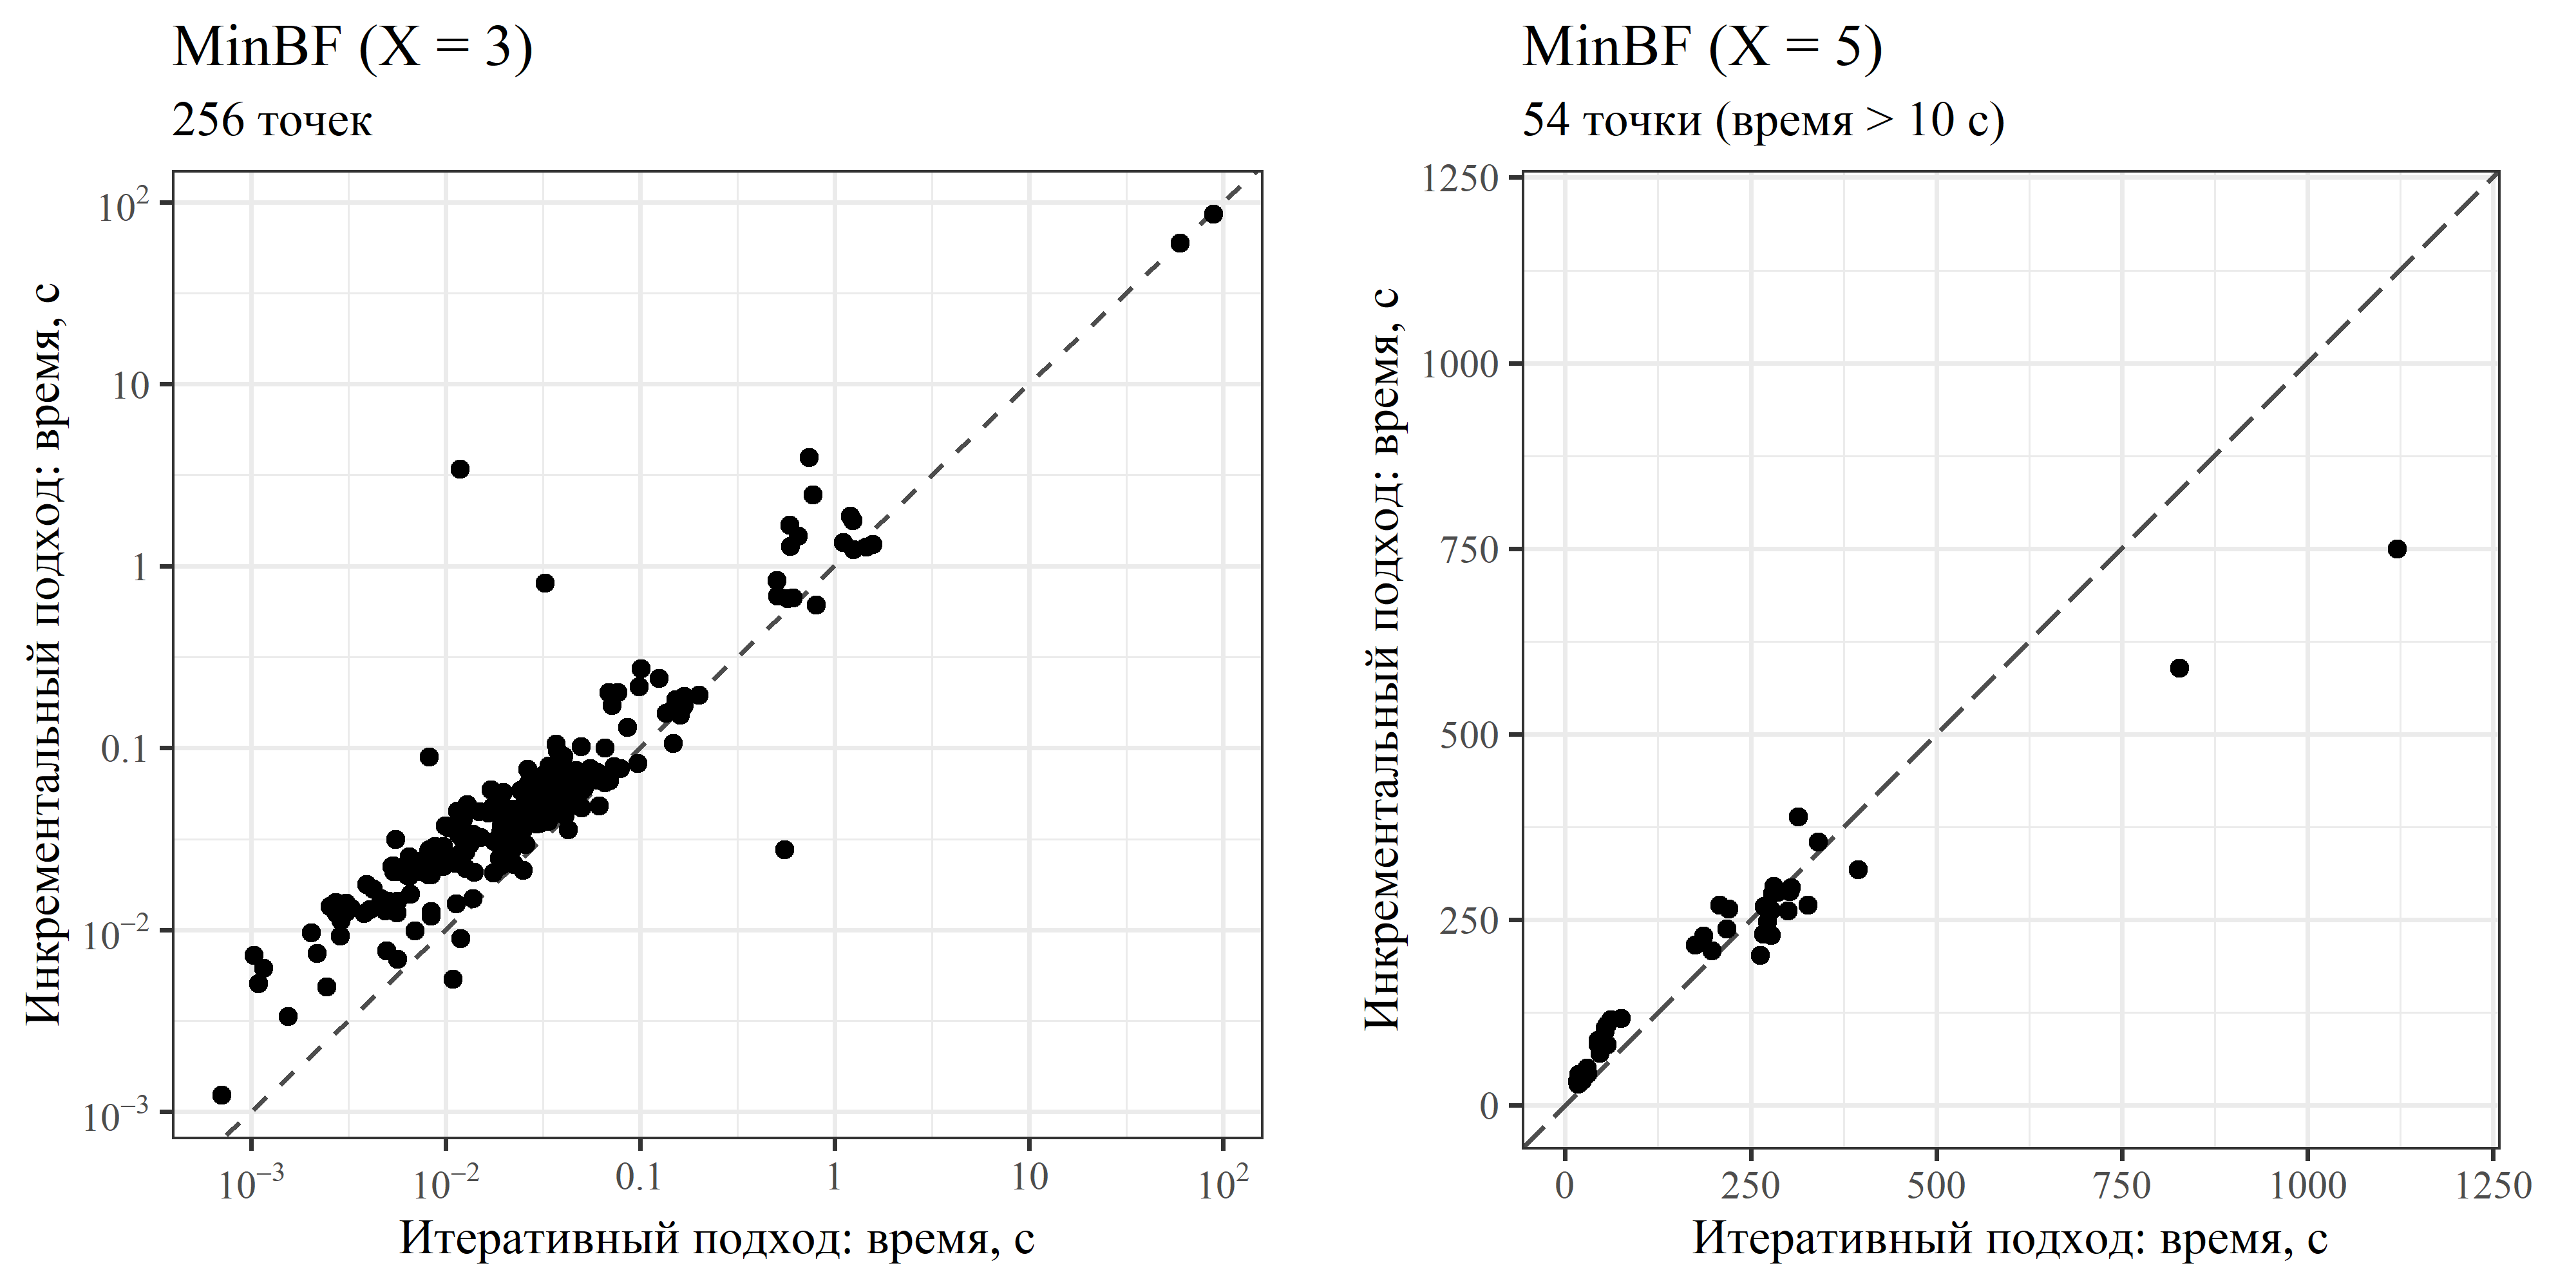
\includegraphics[max width=\linewidth]{minbf.png}
    \caption{Графики сравнения времени работы алгоритма синтеза минимальной булевой формулы (слева \--- от трех переменных, справа \--- от пяти переменных) для двух подходов: итеративный (горизонтальная ось) и инкрементальный (вертикальная ось). Время работы указано в секундах (слева \--- на логарифмической шкале). Каждая точка на графике соответствует булевой функции. На правом графике показаны только точки со временем работы, превышающим 10 секунд.}
    \label{fig:minbf}
\end{figure}

Можно заметить, что большинство минимальных формул для функций от трех переменных были найдены менее, чем за одну секунду \--- сравнение на таких масштабах времени в контексте решения NP-трудных задач не является целесообразным. Поэтому были проведен дополнительный набор экспериментов на данных большей размерности и более «сложных» булевых функциях \--- от $X = 5$ переменных. Результаты приведены на \emph{Рис. 1} (справа), где показаны только точки со временем работы, превышающим 10 секунд (всего 54 точки). Данный график \--- а именно, точки в правой части графика под базовой линией \--- позволяет судить о том, что инкрементальный подход действительно обеспечивает лучшую производительность в рассмотренной задаче синтеза минимальной булевой формулы.



\section{Задача проверки эквивалентности булевых схем}
\label{sub:lec}

Задача проверки эквивалентности булевых схем (Logical Equivalence Checking \--- LEC) является одной из ключевых комбинаторных проблем в автоматизации проектирования электроники.
В этом разделе даны основные понятия о LEC, которые будут использованы в дальнейшем.

Рассмотрим две булевы схемы $S_f$, $S_h$, определяющие функции $f, h: \{0,1\}^n \to \{0,1\}^m$.
Задача LEC заключается в том, чтобы определить, являются ли две заданные схемы эквивалетными, то есть обладают одинаковыми выходами на всех возможных входах, что выражается в том, что соответствующие функции поточечно равны, $f \cong h$.
Задача LEC может быть сведена к задаче выполнимости булевых формул (SAT), ниже это показано на примерах.

\begin{figure}[ht]
    \centering
    \subfile{tex/tikz-glued}
    \caption{Склеенная схема $S_{f \glue h}$, построенная с использованием одного и того же набора входов для двух схем $S_f$ и $S_h$}
    \label{fig:glued}
\end{figure}

Используя $S_f$ и $S_h$, построим новую схему, обозначаемую $S_{f \glue h}$ (см. Рисунок~\ref{fig:glued}), которая получается из $S_f$ и $S_h$ путем \enquote{склейки} вместе входных вершин \--- обозначим её $S_{f \glue h}$.
Она имеет тот же набор входов $\Vin$ как и $S_f$ и $S_h$, и определяет следующую функцию:
\begin{equation}\label{eq:f-glue-h}
    f \glue h \colon \{0,1\}^n \to \{0,1\}^{2m}
\end{equation}
Обозначим через $\Vout_f$ и $\Vout_h$ множества выходов схем $S_f$, $S_h$, а через $Y_f = \{y_1^f, \dots, y_m^f\}$ и $Y_h = \{y_1^h, \dots, y_m^h\}$ множества переменных, связанных с вершинами из $\Vout_f$ и $\Vout_h$ соответственно, упорядоченные согласно семантике схем.
Теперь рассмотрим формулу $(y_1^f \xor y_1^h) \lor \dots \lor (y_m^f \xor y_m^h)$, которая задает булеву функцию $\mathcal{M} \colon \{0,1\}^{2m} \to \{0,1\}$, называемую \textit{miter}~\cite{brand1983}.
Мы обозначим булеву схему, реализующую функцию $\mathcal{M} \circ (f \glue h)$ как $S_{f \xor h}$ и будем ссылаться на нее как на \textit{miter-схему}.
Рассмотрим формулу
\begin{equation}\label{eq:miter-cnf}
    C_{f\xor h} = C_{f \glue h} \land C(\mathcal{M}) ,
\end{equation}
где $C_{f \glue h}$ \=== шаблонная CNF для функции~\eqref{eq:f-glue-h}, а $C(\mathcal{M})$ выглядит следующим образом:
\begin{align*}
    C(\mathcal{M}) = C(w_1 \equiv (y_1^f \xor y_1^h)) \land \dots \land \\
    \land C(w_m \equiv (y_m^f \xor y_m^h)) \land \\
    \land (w_1 \lor \dots \lor w_m) ,
\end{align*}
где $C(w_j \equiv (y_j^f \xor y_j^h))$, $j\in \{1,\dots,m\}$ \--- CNF-представление булевой функции, заданной формулой $w_j \equiv (y_j^f \xor y_j^h)$.
Из Леммы~\ref{lem1} непосредственно следует, что $S_f$ и $S_h$ эквивалентны тогда и только тогда, когда $C_{f \xor h}$ невыполнима.


\section{Задача генерации тестовых шаблонов для верификации булевых схем}
\label{sub:atpg}

В этом разделе рассматривается задача \textit{автоматической} генерации тестовых шаблонов (Automatic Test Pattern Generation \--- ATPG) для верификации булевых схем.
Сначала вводится понятие модели неисправностей (\textit{fault model}).
Затем формулируется задача генерации шаблонов (ATPG) для комбинационных (\textit{combinational}) булевых схем.
Также упоминается секвенциальная (\textit{sequential}) постановка задачи ATPG для схем с элементами памяти, такими как триггеры (\textit{flip-flops}).
Наконец, кратко рассматриваются классические алгоритмы ATPG, работающие на структуре схемы.
% Представление оставлено кратким, для дальнейшего чтения мы ссылаемся на [JG03].
В~разделе~\ref{sub:sat-atpg} отдельно рассматриваются методы решения задачи ATPG, основанные на сведении к задаче выполнимости (SAT), как наиболее релевантные к текущей работе.

\subsubsection{Модель неисправности Stuck-At}

После производства чипа необходимо проверить его функциональную корректность относительно спецификации схемы на уровне булевых элементов.
Без этой проверки некорректный чип будет доставлен заказчикам, что может привести к неполадкам в конечном продукте. Это, конечно же, недопустимо.
С другой стороны, из-за дефектов материала, вариаций процесса во время производства и~т.\@\:д.\@ возможен широкий диапазон неисправностей.
Но непосредственная проверка всех возможных физических дефектов невозможна.
Поэтому вводится абстракция в виде модели неисправности.
Модель неисправности Stuck-At (SAFM) [BF76] хорошо известна и широко используется на практике.
В этой модели неисправности предполагается, что одна линия застряла на фиксированном значении вместо зависимости от значений входов.
Когда линия застряла на значении~0, это называется неисправностью stuck-at-0 (SA0).
Аналогично, если линия застряла на значении 1, это называется неисправностью stuck-at-1 (SA1).

% TODO: \begin{example}
\textbf{Пример.}
Рассмотрим схему, показанную на рисунке 27.7(a). Когда на линии d вводится неисправность SA0, получается неисправная схема, показанная на рисунке 27.7(b). Выход элемента И отключается, и вход элемента ИЛИ постоянно принимает значение 0.

Помимо SAFM было предложено ряд других моделей неисправностей, например, клеточная модель неисправностей [Fri73], где меняется функция одного элемента, или модель мостовой неисправности [KP80], где предполагается, что две линии устанавливаются в одно значение.
Эти модели неисправностей в основном охватывают статические физические дефекты, такие как обрывы или замыкания.
Динамические эффекты охватываются моделями неисправностей задержки.
В~модели неисправности по задержке пути [Smi85] одна неисправность означает, что изменение значения вдоль пути от входов к выходам в схеме не приходит в течение времени цикла тактового сигнала.
Вместо путей модель неисправности задержки на входах элементов [HRVD77, SB77] учитывает задержку в элементах.

Далее рассматривается только SAFM из-за его высокой значимости в практических применениях.
Эту значимость можно объяснить двумя наблюдениями: количество неисправностей имеет порядок размера схемы, и моделирование неисправностей в SAFM относительно просто, то есть для статической модели неисправностей вычислительная сложность генерации тестовых шаблонов ниже по сравнению с динамическими моделями неисправностей.

\subsubsection{Комбинационный ATPG}

Автоматическая генерация тестовых шаблонов (ATPG) \--- это задача определения всех набора тестовых шаблонов для заданной схемы с учетом модели неисправностей.
Тестовый шаблон для конкретной неисправности \--- это назначение на основные входы схемы, которое приводит к различным выходным значениям в зависимости от наличия неисправности.
Вычисление булевой разности между бездефектной и неисправной схемами дает все тестовые шаблоны для конкретной неисправности.
Эта конструкция аналогична схеме \textit{miter}~\cite{brand1983}, поскольку ее можно использовать для проверки эквивалентности комбинационных схем.

% TODO: \begin{example}
\textbf{Пример.}
Снова рассмотрим неисправность SA0 в схеме на рисунке 27.7.
Назначение входов $a = 1$, $b = 1$, $c = 1$ приводит к значению выхода $f = 1$ для корректной схемы и к значению выхода $f = 0$ в случае наличия неисправности.
Поэтому это назначение входов является тестовым шаблоном для неисправности SA0 на линии~$d$.
Конструкция для вычисления булевой разности бездефектной и неисправной схем показана на рисунке 27.8.

Когда тестовый шаблон существует для конкретной неисправности, эта неисправность классифицируется как \textit{тестируемая} (\textit{testable}).
Если тестовый шаблон отсутствует, неисправность называется \textit{избыточной} (\textit{redundant}).
Проблема классификации неисправности как тестируемой или избыточной является NP-полной.
Задача ATPG заключается в классификации всех неисправностей и создании набора тестовых шаблонов, содержащего хотя бы один тестовый шаблон для каждой испытуемой неисправности.

% TODO: \subsubsection{Секвенциальный ATPG}

Генерация тестовых шаблонов для схем, содержащих элементы состояния (памяти), такие как триггеры (\textit{flip-flops}), вычислительно более сложна, потому что элементы памяти не могут быть непосредственно установлены в определенное значение.
Вместо этого поведение схемы во времени должно рассматриваться во время ATPG.
Было предложено ряд инструментов, которые непосредственно решают эту секвенциальную проблему, например, HITEC [NP91].
Но на практике получаемая модель часто слишком сложна для обработки с помощью инструментов ATPG.
Поэтому обычно рассматривается полный режим сканирования для преодоления этой проблемы путем подключения всех элементов состояния в цепочку сканирования [WA73, EW77].
В режиме тестирования цепочка сканирования объединяет все элементы состояния в сдвиговый регистр, в нормальном режиме работы элементы состояния управляются обычной логикой в схеме.
В результате элементы состояния могут рассматриваться как основные входы и выходы для тестирования, и получается комбинационная постановка задачи ATPG, уже рассмотренная выше.

% TODO: \subsubsection{Классические алгоритмы ATPG}

% TODO


\section{Задача булевой выполнимости}
\label{sec:sat}

Задача выполнимости булевых формул (Boolean satisfiability problem \--- SAT) формулируется следующим образом~\cite{handbook-sat}: для произвольной булевой формулы~$\phi(x_1, \dotsc, x_n)$ необходимо определить, существует ли подстановка значений переменных $X_\text{SAT}$, при которой формула становится истинной, то есть, формально, $\exists X_\text{SAT} \in \{0,1\}^n : \phi(X_\text{SAT}) = 1$.
Если такая подстановка существует, то она называется \textit{удовлетворяющей} (\textit{satisfying assignment}; также используются термины \textit{модель} и \textit{интерпретация}), а формула~$\phi$ называется \textit{выполнимой} (\textit{SATisfiable}).
В~противном случае, если удовлетворяющая подстановка не существует, $\phi$~называется \textit{невыполнимой} (\textit{UNSATisfiable}).

Задача SAT является первой задачей, для которой была доказана NP-полнота~\cite{cook}.
\todo{Описание универсальности задачи SAT}

% \subsection{Базовые определения}
% \label{sub:sat-definitions}

% \todo{Литерал, дизъюнкция, конъюнкция, КНФ, ДНФ}

Если булева формула $\phi$ представлена в конъюктивной нормальной форме (КНФ), то соответствующую задачу называют CNF-SAT.
Любая булева формула может быть преобразована в эквивалентную КНФ, однако при этом размер формулы может увеличиться экспоненциально, например:
\[
    \text{$n$ конъюнкций}
    \left\{
    \begin{aligned}
        & (x_1 \land y_1) \lor \\
        & (x_2 \land y_2) \lor \\
        & ~\dots \\
        & (x_n \land y_n)
    \end{aligned}
    \right.
    \quad
    \xRightarrow{\text{КНФ~}}
    \quad
    \left.
    \begin{aligned}
        & (x_1 \lor x_2 \lor \dotsb \lor x_n) \land \\
        & (y_1 \lor x_2 \lor \dotsb \lor x_n) \land \\
        & ~\dotsb \\
        & (y_1 \lor y_2 \lor \dotsb \lor y_n)
    \end{aligned}
    \right\}
    \text{$2^n$ дизъюнкций}
\]
С помощью преобразований Цейтина~\cite{tseitin1970} возможно привести любую булеву формулу в КНФ \--- с сохранением выполнимости (\textit{equisatisfiable CNF}), но с добавлением новых переменных (\textit{auxiliary variable}) \--- при этом размер формулы увеличится лишь линейно.
В данной работе подразумевается, что все булевы выражения, кодирующие задаваемые ограничения, подвергаются либо эквивалентным логическим преобразованиям, либо преобразованиям Цейтина, то есть по итогу представляются в виде КНФ.


\section{Основные алгоритмы решения SAT}

С учетом сказанного в предыдущем разделе, везде далее под задачей о булевой выполнимости (она же SAT) в распознавательном варианте понимается задача распознавания выполнимости произвольной булевой формулы в КНФ. SAT является исторически первой NP-полной задачей. Данный факт был установлен С.А. Куком (без привлечения точного определения NP-полноты) в статье {[}\hl{1}{]}, которая является основополагающей работой для структурной теории сложности алгоритмов. Помимо распознавательного варианта далее нас будет интересовать поисковый вариант SAT \--- когда требуется распознать выполнимость КНФ, и в случае ее выполнимости найти произвольный выполняющий набор. Данная задача, соответственно, NP-трудна. Сказанное означает, что в предположении $P \neq NP$, SAT не может быть решена в общем случае за полиномиальное время. При всем этом существует масса разнообразных аргументов в пользу того, что SAT (как и многие другие NP-трудные задачи) не является сложной в большинстве своих частных случаев. Именно этот факт позволяет использовать современные алгоритмы решения SAT в задачах, комбинаторная размерность которых может быть колоссальной. Так, в символьной верификации удается успешно решать SAT в отношении КНФ, включающих миллионы дизъюнктов. Число переменных, встречающихся в таких КНФ, может исчисляться десятками и сотнями тысяч. В настоящем разделе мы кратко коснемся алгоритмов решения SAT, которые могут применяться к обращению функций вида (1)-(2). Существуют два больших класса алгоритмов решения SAT \--- полные и неполные. Неполные алгоритмы плохо подходят или не подходят совсем для решения задач, в которых требуется доказывать невыполнимость (соответственно, например, для символьной верификации). Однако они вполне могут использоваться для обращения функций.

В настоящей работе основным вычислительным инструментом являются полные алгоритмы решения SAT. Именно такие алгоритмы позволяют точно решать задачи верификации автоматов и булевых схем, то есть находить решение, если оно существует, либо гарантировать его отсутствие при заданных параметрах, что в том числе позволяет точно решать задачу минимизации.


\subsection{Неполные алгоритмы решения SAT}

Неполные алгоритмы решения SAT не гарантируют ответ SAT/UNSAT за конечное время для произвольной КНФ. Существует целый ряд различных концепций, лежащих в основе таких алгоритмов. Статья {[}\hl{2}{]} представляет собой детальный обзор по данному вопросу, содержащий ключевые ссылки. В дальнейшем нас будут интересовать только те неполные алгоритмы решения SAT, в основе которых лежит идеология локального поиска или (в отдельных случаях) эволюционные стратегии. В таких алгоритмах задача SAT в отношении КНФ $C$ над множеством из $n$ переменных, состоящей из $m$ дизъюнктов, рассматривается в форме задачи максимизации псевдобулевой функции

$f_{C} \colon \left\{ 0,1 \right\}^{n} \to \left\{ 0,1,\ldots,m \right\}$. (9)

Напомним здесь, что псевдобулевой (см, например, {[}\hl{3}{]}) называется любая функция вида

$f \colon \left\{ 0,1 \right\}^{n} \to \mathbf{R}\ .$ (10)

На произвольном наборе $\alpha \in \left\{ 0,1 \right\}^{n}$ значение функции (9) равно числу дизъюнктов в $C$, которые на этом наборе обращаются в 1. Фактически в данном случае мы рассматриваем задачу SAT в оптимизационной постановке, известной как MaxSAT.

Рассматривая $\left\{ 0,1 \right\}^{n}$ в роли пространства поиска, можно ввести на нем \textit{функцию окрестностей} {[}\hl{4}{]} $\aleph:\left\{ 0,1 \right\}^{n} \to 2^{\left\{ 0,1 \right\}^{n}}$. Проще всего для этой цели использовать метрику Хэмминга {[}\hl{5}{]}, в рамках которой для произвольной точки $\alpha \in \left\{ 0,1 \right\}^{n}$ ее окрестность Хэмминга радиуса $r,r \geq 1$, определяется следующим образом:

$\aleph_{r}(\alpha) = \left\{ \alpha^{'} \in \left\{ 0,1 \right\}^{n}:\rho_{H}\left( \alpha,\alpha^{'} \right) \leq r \right\}$. (11)

В (11) через $\rho_{H}(\alpha,\alpha')$ обозначено расстояние Хэмминга между словами $\alpha$ и~$\alpha'$. Чаще всего рассматриваются окрестности радиуса~1. В такой постановке для решения SAT и MaxSAT может использоваться, без преувеличения, огромный арсенал методов локального поиска. Мы проиллюстрируем общую идею, лежащую в основе таких методов, на примере простейшего алгоритма, известного как «Восхождение к вершине» (\enquote{\textit{Hill Climbing}} \--- далее HC) {[}\hl{6}{]}. Опишем вариант HC, применимый для максимизации произвольной псевдобулевой функции вида (10).

\begin{enumerate}
\item
  выбираем (вообще говоря, произвольным образом, например, случайно в соответствии с равномерным распределением на $\left\{ 0,1 \right\}^{n}$) стартовую точку $\alpha_{0} \in \left\{ 0,1 \right\}^{n}$, вычисляем $f\left( \alpha_{0} \right)$; считаем $\alpha_{0}$ текущей точкой, а $f \left( \alpha_{0} \right)$ текущим значением $f$;

\item
  пусть $\alpha \in \left\{ 0,1 \right\}^{n}$ \--- текущая точка;

  обходим в некотором порядке $\aleph_{1}(\alpha)\setminus\left\{ \alpha \right\}$, вычисляя для каждой точки $\alpha'$ из данного множества $f(\alpha')$. Если найдена такая точка $\alpha^{'} \in \aleph_{1}(\alpha) \setminus \left\{ \alpha \right\}$, что $f(\alpha') > f(\alpha)$, перейти на шаг 2, в противном случае перейти на шаг 3;

\item
  $\alpha \gets \alpha'$, $f(\alpha) \gets f(\alpha')$, перейти на шаг 1;

\item
  $\left( \alpha,f(\alpha) \right)$ \--- локальный максимум функции $f$ на $\left\{ 0,1 \right\}^{n}$ (поскольку для любой $\alpha^{'} \in \aleph_{1}(\alpha)\setminus \left\{ \alpha \right\}$ имеет место $f(\alpha') \leq f(\alpha)$); в этом случае алгоритм либо останавливается и выдает в качестве ответа $\left( \alpha, f(\alpha) \right)$, либо запускает некоторую процедуру выхода из локального максимума.
\end{enumerate}

Для выхода из локальных экстремумов можно дополнять приведенный выше базовый алгоритм различными техниками, основанными на эвристических и метаэвристических соображениях. Зачастую, выйдя из точки локального экстремума, можно оказаться в точке с худшим значением $f$. Такого сорта «выпрыгивания» из локальных экстремумов могут осуществляться в процессе поиска неоднократно. В этом случае обычно хранится точка с самым лучшим значением функции $f$, достигнутым за все историю поиска. Такое значение называется \textit{рекордом} (\textit{best known value} \--- BKV). Современные техники выхода из локальных экстремумов позволяют даже при решении весьма трудных задач многократно улучшать рекорд в процессе поиска. Если некоторое количество попыток выхода из локальных экстремумов не дает улучшения текущего рекорда $f^{*}$, достигнутого в точке $\alpha^{*}$, то алгоритм останавливается и выдает в качестве ответа пару $\left( \alpha^{*},f^{*} \right)$.

Предположим, что HC применяется к задаче максимизации произвольной функции вида (9). Легко понять, что даже если дополнить HC какой-либо процедурой выхода из точек локального максимума, это не позволит безошибочно распознавать невыполнимость невыполнимых КНФ. С другой стороны, если рассматривается КНФ с большим числом выполняющих наборов, то HC (даже в самом простом варианте) может случайно натолкнуться на такой набор за приемлемое время. Известный пример данного типа \--- успешное использование HC для решения SAT в отношении КНФ, кодирующих задачу размещения $k$ ферзей на шахматной доске размерности $k \times k$ {[}\hl{7}{]}. Однако, к сожалению, HC и известные его модификации напрямую неприменимы к КНФ, кодирующим обращение интересных с практической точки зрения криптографических функций. Причем это верно даже в отношении КНФ с огромным числом выполняющих наборов \--- например, для КНФ, кодирующих задачи обращения криптографических хеш-функций.

Если некоторый алгоритм локального поиска, решающий задачу максимизации функции вида (9), слишком долго не может улучшить текущий рекорд $\left( \alpha,f_{C}(\alpha) \right)$, где $f_{C}(\alpha) < m$, то данный алгоритм можно остановить с ответом «UNSAT» в отношении КНФ $C$. Этот ответ может оказаться ошибочным. Однако существуют специальные техники рандомизации локального поиска, использование которых позволяет оценивать вероятность ошибки указанного типа и даже снижать эту вероятность за счет выполнения алгоритмом большого числа некоторых случайных шагов. Один из самых известных примеров такого рода \--- алгоритм, предложенный У.~Шёнингом в {[}\hl{8}{]}. Данный алгоритм решает задачу о выполнимости произвольной $k$-КНФ, $k \geq 2$, то есть КНФ, каждый дизъюнкт которой имеет длину~$k$. Алгоритм Шёнинга пытается улучшить значение функции (9), достигнутое в точке $\alpha \in \left\{ 0,1 \right\}^{n}$, за счет случайного выбора и модификации тех дизъюнктов в КНФ $C$, которые обращаются в 0 на наборе $\alpha$. Получаемый в результате процесс интерпретируется в рамках хорошо изученной в теории вероятностей модели случайных блужданий {[}\hl{9}{]}. Как результат, если алгоритм Шёнинга, сделав $O\left( n \cdot \left( 2 - \frac{2}{k} \right)^{n} \right)$ простых случайных действий, не находит выполняющий набор, то вероятность ошибиться, заключив, что $C$~невыполнима, не превосходит $1 - \frac{1}{p(n)}$, где через $p( \cdot )$ обозначен некоторый полином. Очевидно, что если повторение упомянутого выше списка действий, скажем, $n \cdot p(n)$ раз не дает выполняющий набор, то заключение о невыполнимости $C$ будет справедливым с вероятностью, которая близка к $1 - e^{- n}$. Идеи, лежащие в основе алгоритма Шёнинга, позволили для SAT в отношении 3-КНФ построить нетривиальные верхние оценки сложности, которые долгое время оставались лучшими среди аналогичных по смыслу оценок (см. {[}\hl{10}{]}, {[}\hl{11}{]}).

Алгоритмы, в которых базовые схемы локального поиска (например, HC) дополняется различными стратегиями рандомизации, относятся к классу, известному как \textit{Stochastic Local Search methods} (SLS). К большому сожалению, имеющиеся на сегодняшний день SLS-алгоритмы плохо подходят для обращения криптографических функций. Как будет показано далее, лучшие такие алгоритмы позволяют успешно решать задачи криптоанализа лишь весьма простых генераторов ключевого потока.

\subsection{Полные алгоритмы решения SAT}

Алгоритм решения SAT называется полным, если для любой КНФ $C$ он за конечное число шагов выдает верный ответ вида SAT/UNSAT. Как и в ситуации с неполными, для построения полных алгоритмов решения SAT можно использовать множество различных базовых концепций. Так, довольно естественно решать SAT, основываясь на широко применяемой в комбинаторной оптимизации идеологии ветвей, границ и отсечений {[}\hl{12}{]}. Хорошо известна сводимость SAT к задаче 0-1-Целочисленное линейное программирование (0-1-ЦЛП), после осуществления которой можно использовать для решения полученной задачи из семейства 0-1-ЦЛП богатый набор программных средств. Также довольно просто перейти от SAT к задаче поиска решений системы алгебраических уравнений степени не выше 2 над полем $GF(2)$. К таким системам можно применять известный алгоритм Б. Бухбергера (он же «метод баз Грёбнера») {[}\hl{13}{]}, а также специальные техники работы с разреженными квадратичными системами над $GF(2)$ (см., например, {[}\hl{14}{]}, {[}\hl{15}{]}).

Многие авторы сходятся во мнении, что лучших результатов в решении трудных вариантов SAT из целого ряда областей, среди которых символьная верификация и криптоанализ, удается добиться за счет использования алгоритмов, относящихся к направлению, которое правильнее всего назвать «Вычислительная логика». Ранние алгоритмы из данного класса лежали в основе первых программных реализаций систем автоматического доказательства теорем \textit{(Automated theorem proving, ATP)}. Одним из таких алгоритмов был «метод Девиса-Патнема» (Davis-Putnam method) {[}\hl{16}{]}. Усовершенствованная версия данного алгоритма, известная как DPLL (от фамилий Davis, Putnam, Logemann, Loveland) {[}\hl{17}{]}, до настоящего момента продолжает использоваться в основе высокоэффективных полных SAT-решателей. DPLL представляет собой обход дерева поиска, в рамках которого выход из тупиковых ветвей организован в форме процедуры, называемой \textit{хронологическим бэктрекингом} (\textit{chronological backtracking}) Остановимся подробнее на тех деталях DPLL, которые потребуются нам в дальнейшем.


\subsection{Алгоритм DPLL}

Пусть $C$ \--- произвольная КНФ над множеством переменных $X$. Пусть $S \subset L_{X}$ \--- произвольное множество литералов над переменными из~$X$, которое не содержит контрарных литералов. Пусть $X_{S}$ \=== множество, включающее все те переменные из $X$, литералы над которыми содержатся в $S$ ($X_{S} \subseteq X$). Рассмотрим отображение
$\sigma \colon X_{S} \to \left\{ 0,1 \right\}\ $,
заданное по следующему правилу:
\(
    \sigma\left( x \in X_{S} \right) = \left\{ \begin{array}{r}
    1,\ x \in S\ \ \ \ \  \\
    0,\ \neg x \in S\ .
    \end{array} \right.\
\) (12)

Иными словами, отображение (12) связывает с выбираемыми из $L_{X}$ литералами значения соответствующих переменных: выбор литерала $x$ интерпретируется как присвоение переменной $x$ значения 1, выбор же $\neg x$, соответствует принятию $x$ значения 0. Множество $S$ будем называть списком литералов, выбранных из $L_{X}$. Теперь опишем собственно алгоритм DPLL.

На начальном шаге список выбранных литералов пуст. Выберем (вообще говоря, произвольный) литерал $l_{1} \in L_{X}$, поместим его в список $S_{1}$ и рассмотрим КНФ $l_{1} \land C$. Удалим из данной КНФ каждый дизъюнкт вида $\left( l_{1} \lor D \right)$, а из каждого дизъюнкта вида $\left( \neg l_{1} \lor D \right)$ удалим литерал $\neg l_{1}$ (здесь через $D$ обозначен произвольный непустой дизъюнкт над $X$). Обозначим результирующую КНФ через $C'$. Будем говорить, что данная КНФ получена из $l_{1} \land C$ в результате применения правила \textit{единичного дизъюнкта} (Unit Propagation rule, UP, {[}\hl{18}{]}) к $C$ и литералу $l_{1}$. Заметим, что если в $C$ содержался дизъюнкт вида $D = \left( \neg l_{1} \lor l' \right)$, то удаление из $D$ литерала $\neg l_{1}$ дает единичный дизъюнкт, состоящий из литерала $l'$. В описанной ситуации литерал $l_{1}$ называют \textit{угаданным}, а про литерал $l'$ говорят, что он был \textit{выведен по правилу единичного дизъюнкта}. К КНФ $C'$ и литералу $l'$ можно снова применить правило единичного дизъюнкта. Если в результате применения UP вывелось несколько литералов, они все ставятся в очередь, после чего к ним и соответствующим КНФ последовательно применяется UP.

Пусть $S_{k} = \left\{ l_{1},\ldots,l_{k} \right\}$ \--- список угаданных литералов. Обозначим через ${\widetilde{S}}_{k}$ список всех литералов, которые были выведены по правилу UP в соответствии с описанной выше процедурой. Пусть $C_{k}$ \=== полученная в результате КНФ. Проанализируем несколько ситуаций, которые могут при этом возникнуть.

\begin{enumerate}
\item
  Пусть ${\widetilde{S}}_{k}$ не содержит контрарных литералов, а $C_{k}$ содержит только единичные дизъюнкты. Тогда $C$ выполнима. Несложно показать, что в этом случае существует выполняющий $C$ набор, в котором значения части (или всех) переменных определяются при помощи отображения (12), применяемого к литералам из $S_{k} \union {\widetilde{S}}_{k}$ .
\item
  Пусть ${\widetilde{S}}_{k}$ не содержит контрарных литералов, а $C_{k}$ содержит дизъюнкты длины не менее 2. Пусть ${\widetilde{C}}_{k}$ \=== КНФ, составленная из этих дизъюнктов, а ${\widetilde{X}}_{k}$ \=== множество переменных, встречающихся в ${\widetilde{C}}_{k}$. Тогда выберем из $L_{{\widetilde{X}}_{k}}$ произвольный литерал $l_{k + 1}$, построим список $S_{k + 1} = S_{k} \union \left\{ l_{k + 1} \right\}$ и применим UP к ${\widetilde{C}}_{k}$ и $l_{k + 1}$.
\item
  Список ${\widetilde{S}}_{k}$ содержит контрарные литералы, то есть пару вида $(l,\neg l)$ для некоторого $l \in L_{X}$. В этой ситуации будем говорить, что список угаданных литералов $S_{k}$ породил конфликт. Сам по себе конфликт еще не означает, что исходная КНФ невыполнима \--- вполне возможно, что она выполнима, но были угаданы такие литералы, что сочетание соответствующих им в смысле отображения (12) значений переменных не встречается ни в одном из выполняющих $C$ наборов.
\end{enumerate}

Пусть $S_{k} = \left\{ l_{1},\ldots,l_{k} \right\}$ \--- список угаданных литералов, такой что после угадывания $l_{k}$ по UP был выведен конфликт. В этой ситуации перейдем от списка $S_{k}$ к списку $S_{k}^{'} = \left\{ l_{1},\ldots,\neg l_{k} \right\}$, помечая литерал $\neg l_{k}$ как «инвертированный». Предположим, что для некоторого $k$ оба списка $S_{k} = \left\{ l_{1},\ldots,l_{k} \right\}$ и $S_{k}^{'} = \left\{ l_{1},\ldots,{\neg l}_{k} \right\}$ порождают конфликты. Пусть $l_{r}$ \=== ближайший предшествующий $l_{k}$ литерал в списке $S_{k}$, который ранее не был инвертирован. Тогда новым списком является $S_{r}^{'} = \left\{ l_{1},\ldots,{\neg l}_{r} \right\}$ (везде здесь предполагалось, что $k,r \geq 2$).

Описанная выше процедура перехода к списку $S_{r}^{'}$ называется хронологическим (обычным) бэктрекингом. Можно заметить, что процесс бэктрегинга соответствует обходу с возвратом бинарного дерева специального вида. Вершинам этого дерева приписаны переменные из $X$. Из произвольной вершины, которой приписана переменная $x$, выходит два ребра, символизирующие литералы $x$ и $\neg x$. Корню данного дерева приписана переменная, над которой берется литерал $l_{1}$. Произвольная ветвь соответствует некоторому списку угаданных литералов. Если такой список порождает конфликт, то соответствующую ветвь назовем тупиковой.

Если для некоторого $k$ списки $S_{k}$ и $S_{k}^{'}$ порождают конфликты, и при этом все литералы, предшествующие $l_{k}$, включая первый, были инвертированы, то каждая ветвь описанного выше дерева поиска является тупиковой. Легко понять, что данный факт означает невыполнимость КНФ $C$. Также в силу всего сказанного выше можно заметить, что число вершин в таком дереве поиска не превосходит $M = 2^{n + 1} - 1$. Отметим, что в реальности это число может быть существенно меньше за счет большого числа литералов, выведенных по UP. Таким образом, применив UP не более $M$ раз, мы либо достигнем ситуации, описанной в пункте 1, и это будет означать, что $C$ выполнима, либо докажем невыполнимость $C$. Все сказанное означает полноту алгоритма DPLL.

\subsection{Концепция CDCL и базирующиеся на ней современные SAT-решатели}

Концепция решения SAT, известная сегодня как Conflict Driven Clause Learning (CDCL), включает в себя ряд важных техник, дополняющих алгоритм DPLL. Первая и главная из них позволяет записывать информацию о конфликте, который возник в процессе обхода дерева поиска, в виде специальным образом построенного дизъюнкта. Такой дизъюнкт называется \textit{конфликтным} (conflict-induced clause). Если $C$ \=== исходная КНФ, а $D$ \=== конфликтный дизъюнкт, то имеет место: $C \to D$, то есть $D$ \=== это логическое следствие (импликация) из~$C$. Соответственно, КНФ~$C$ выполнима тогда и только тогда, когда выполнима КНФ~$C \land D$.

Конфликтные дизъюнкты можно строить различными способами. Приведем простейший пример. Пусть список угаданных литералов $S_{k} = \left\{ l_{1},\ldots,l_{k} \right\}$ породил конфликт в рамках DPLL. Построим следующий конфликтный дизъюнкт: $D = \left( \neg l_{1} \lor \ldots \lor \neg l_{k} \right)$. Данный дизъюнкт запрещает одновременный выбор всех литералов из списка $S_{k}$. Рассмотрим КНФ $C \land D$ ($C$ \=== исходная КНФ). Если мы применим к КНФ $C \land D$ DPLL, используя список угаданных литералов $S_{k - 1} = \left\{ l_{1},\ldots,l_{k - 1} \right\}$, то единичный дизъюнкт $\neg l_{k}$ будет выведен по правилу UP. В этом случае говорят, что вывод литерала $\neg l_{k}$ индуцирован конфликтом. Очень важно, что в данном случае литерал ${\neg l}_{k}$ не угадывается, а выводится по правилу UP на основе информации, полученной в результате анализа конфликта.

Впервые идея использовать конфликтные дизъюнкты для записи информации о тупиковых ветвях в DPLL-поиске была предложена в конференционной статье Ж. Маркеша-Сильвы и К. Сакаллы в 1996 году (см. {[}\hl{19}{]}). В более детальном виде она была представлена этими же авторами в журнальной статье {[}\hl{20}{]}. По сути, именно в этих двух работах были заложены основы концепции CDCL. Еще одна важная техника, которая была описана в {[}\hl{19}{]},{[}\hl{20}{]}, заключается в использовании для представления процесса решения SAT специальных графов, называемых \textit{графами вывода} (\textit{implication graph}). Граф вывода позволяет эффективно выявлять литералы (причем, что важно, как угаданные, так и выведенные по UP), которые ответственны за рассматриваемый конфликт. Графы вывода очень информативны. Разные способы обхода IG соответствуют различным эвристикам формирования конфликтных дизъюнктов. Некоторые такие эвристики также были приведены в {[}\hl{19}{]},{[}\hl{20}{]}.

Основное концептуальное отличие CDCL~от DPLL заключается в том, что CDCL~использует память для хранения информации о ходе поиска в форме конфликтных дизъюнктов. Это позволяет вместо хронологического бэктрекинга в ряде случаев осуществлять \textit{нехронологический бэктрекинг} (\textit{non-chronological backtracking}), называемый также \textit{бэкджампингом} (backjumping). Бэкджампинг \--- это ситуация, когда после анализа конфликта откат в списке угаданных литералов происходит не к ближайшему (от конфликта) литералу, который не был ранее инвертирован, а к угаданному еще раньше (иногда существенно раньше). Во многих случаях бэкджампинг позволяет эффективно отсекать значительные части дерева поиска, запрещая при помощи конфликтных дизъюнктов последующий поиск в этих областях. Первым SAT-решателем, фактически использующим CDCL, был GRASP {[}\hl{19}{]}.

Следующий шаг был сделан в работах {[}\hl{21}{]},{[}\hl{22}{]}, где были введены еще несколько важных техник, дополняющих базовый CDCL. Так, в {[}\hl{21}{]} был описан механизм выбора порядка угадывания литералов, основанный на их «мере конфликтности». Соответствующая эвристика получила называние VSIDS (Variable State Independent Decaying Sum). Также в {[}\hl{21}{]} была описана весьма эффективная техника итеративного применения правила UP, использующая т.н. \enquote{ленивые} (\textit{lazy}) структуры данных, известные как \textit{watched literals}, применяются в настоящее время в большинстве CDCL SAT-решателей. Еще одно важное достижение {[}\hl{21}{]} \--- экспериментальная аргументация пользы рестартов. В статье {[}\hl{22}{]} было проведено детальное исследование различных способов построения конфликтных дизъюнктов за счет анализа графов вывода. На основе результатов работ {[}\hl{21}{]},{[}\hl{22}{]} был построен решатель zchaff \--- первый по-настоящему высокоэффективный SAT решатель, базирующийся на концепции CDCL. С использованием zchaff еще в 2002 году удавалось решать задачи криптоанализа некоторых поточных шифров существенно быстрее простого перебора.

В 2003 году в работе {[}\hl{23}{]} были описаны общие принципы построения высокоскоростного CDCL SAT-решателя с эффективно модифицируемой архитектурой. Исходный код соответствующего решателя, получившего название minisat, был представлен авторами {[}\hl{23}{]} в открытом доступе. Решатель minisat на протяжении многих лет остается де-факто стандартом программной основы эффективных SAT-решателей как широкого профиля, так и нацеленных на конкретную прикладную область. Еще одной важной частью minisat стали процедуры периодической чистки баз конфликтных дизъюнктов. Здесь следует отметить, что грамотно реализованный CDCL в процессе работы может генерировать огромные массивы конфликтной информации. Чрезмерное количество конфликтных дизъюнктов увеличивает число срабатываний правила UP и, как следствие, приводит к падению эффективности вывода. Соответственно, часть конфликтной информации можно попытаться удалить. Однако неудачное удаление конфликтных дизъюнктов может привести к их повторной генерации. В данном контексте особенно ценны эвристики, которые позволяют удалять большое число слабо релевантных конфликтных дизъюнктов. Первые относительно нетривиальные такие эвристики были предложены в статье {[}\hl{24}{]}.

Алгоритмы решения SAT, основанные на CDCL, оказались весьма удачно приспособленными для применения к ним различных концепций распараллеливания. Основными двумя такими концепциями являются т.н. \textit{Portfolio approach} и \textit{Partitioning approach} (далее соответственно, «портфолио-подход» и «подход на основе разбиений»). Детальное сравнение эффективности этих двух подходов предпринято в диссертации А. Хиваринена {[}\hl{25}{]}.

Портфолио-подход предполагает запуск нескольких копий решателя на исходном пространстве поиска, при этом каждая копия начинает работу, используя некоторый набор значений входных параметров SAT решателя (разным копиям соответствуют различные наборы значений параметров). В процессе работы копии решателей могут обмениваться друг с другом конфликтными дизъюнктами. Для достижения высокой скорости такой обмен обычно организуется через оперативную память вычислительного устройства с использованием технологий многопоточного программирования. Соответствующая техника получила название \textit{clause sharing} (\enquote{обмен конфликтными дизъюнктами}). Одна из первых эффективных реализаций обмена конфликтными дизъюнктами была представлена в {[}\hl{26}{]}.

Подход на основе разбиений \textit{(SAT-partitioning)} предполагает разбиение пространства поиска (т.е. фактически множества $\left\{ 0,1 \right\}^{n}$, где $n -$ число переменных в КНФ) на непересекающиеся подобласти, которые обрабатываются независимо друг от друга. Данный подход позволяет организовать решение SAT в параллельной среде со слабо связанными или даже независимыми рабочими процессами (в частности, в грид-средах). Как будет показано далее, подход на основе разбиений дает хорошие результаты при решении SAT-задач, кодирующих криптоанализ блочных и поточных шифров, поскольку естественным образом ассоциируется с атаками, относящимися к классу «угадывай и определяй» (guess and determine) {[}\hl{27}{]}.

Скажем здесь несколько слов по поводу теоретических аргументов эффективности CDCL. Соответствующие результаты относятся к теории сложности пропозициональных доказательств. В этой области исследуется задача доказательства невыполнимости невыполнимой формулы в КНФ. Пусть $C$ \=== произвольная невыполнимая КНФ и $x_{C}$ \=== двоичное слово, представляющее~$C$ в некоторой «разумной» системе кодирования. Пусть $\Sigma_{U} \subset \left\{ 0,1 \right\}^{*}$ \=== множество слов~$x_{C}$ по всем возможным невыполнимым КНФ~$C$. Пусть $A$ \=== произвольный полный алгоритм решения SAT. Любой такой алгоритм называется также системой пропозиционального доказательства (\textit{Propositional proof system}). Получив на вход $x_{C}$, алгоритм $A$ выдает двоичное слово $s$, которое будем называть $A -$ доказательством невыполнимости $C$ (см., например, {[}\hl{28}{]}). Рассмотрим функцию $\omega_{A}:\left\{ 0,1 \right\}^{*} \to \left\{ 0,1 \right\}^{*}$, определенную следующим образом. Если слово является $A -$доказательством невыполнимости некоторой КНФ $C$, то $\omega_{A}$ сопоставляет этому слову слово $x_{C}$. В противном случае выходом $\omega_{A}$ является двоичный код символа $\varnothing$. Несложно понять, что для одной и той же $C$ могут существовать различные $A -$ доказательства ее невыполнимости (особенно хорошо это видно на примере метода резолюций). С~произвольным $x_{C} \in \Sigma_{U}$ свяжем длину кратчайшего $A $\=доказательства невыполнимости $C$. Можно заметить, что если для некоторого $A$ функция длины кратчайшего $A $\=доказательства по всем $x_{C} \in \Sigma_{U}$ растет как полином от~$|x_{C}|$, то $\mathrm{NP} = \mathrm{coNP}$ (см. {[}\hl{29}{]}). Однако для целого ряда алгоритмов несложно указать примеры бесконечных семейств невыполнимых КНФ с полиномиально растущей длиной кратчайшего $A -$доказательства на этих КНФ.

Пусть теперь $A$ и $B$ \=== два полных алгоритма решения SAT. Пусть $C$ \=== произвольная формула из $\Sigma_{U}$. Если существует полиномиальный алгоритм, который произвольное $A -$доказательство невыполнимости $C$ преобразует в $B -$доказательство ее невыполнимости, то говорят, что система доказательств $B$ полиномиально моделирует систему доказательств $A$. Если $A$ полиномиально моделирует $B$, а $B$ полиномиально моделирует $A$, то данные системы доказательств называются полиномиально эквивалентными. Если на некотором (бесконечном) семействе противоречий ${\Sigma'}_{U} \subset \Sigma_{U}$ длина кратчайшего $A -$доказательства растет как полином от длины КНФ, а длина кратчайшего $B -$ доказательства как экспонента, то очевидно, что $B$ не может полиномиально моделировать $A$. Если при этом $A$ полиномиально моделирует $B$, то разумно считать систему $A$ мощнее системы $B$.

В серии работ конца 90-х \-- начала 00-х годов были получены результаты, касающиеся сложности доказательств в системах, связанных с методом резолюций {[}\hl{30}{]}. В данном контексте важнейший для нас результат содержится в статьях {[}\hl{31}{]},{[}\hl{32}{]}, где было показано, что «общая резолюция» (general resolution) в ее пропозициональном варианте полиномиально эквивалентна алгоритму CDCL с рестартами. Данный факт, в частности, означает, что CDCL имеет экспоненциальную сложность. Действительно, в работе {[}\hl{33}{]} было установлено, что общая резолюция экспоненциальна на семействе логических противоречий, известных как «формулы Дирихле» (Pigeon Hole Principle formulas, $PHP_{n}^{n + 1}$, {[}\hl{34}{]}). В силу сказанного выше, это означает, что и CDCL будет иметь на $PHP_{n}^{n + 1}$ экспоненциальную сложность. В то же время, CDCL является более мощной системой доказательств, чем DPLL (см. {[}\hl{31}{]},{[}\hl{32}{]},{[}\hl{34}{]}).

% \subsection{Алгоритм CDCL}
% \label{sub:cdcl}

% Conflict-Driven Clause Learning (CDCL) \--- это расширение классического алгоритма DPLL, включающее в себя механизмы анализа конфликтов и вывода новых дизъюнктов.
% Алгоритм CDCL лежит в основе многих современных SAT-решателей благодаря своей эффективности при решении экземпляров задачи SAT.
% Ниже приводится подробное описание алгоритма CDCL, а также псевдокод для наглядности.

% \todo{Описание алгоритма CDCL}

\begin{algorithm}[H]
    \caption{DPLL Algorithm with Conflict Analysis and Clause Learning}
    \DontPrintSemicolon
    \SetKwInput{Input}{Input}
    \SetKwInput{Output}{Output}
    \SetKwFunction{AnalyzeConflict}{AnalyzeConflict}

    \Input{Boolean formula $F$, current assignment $\sigma$}
    \Output{satisfying assignment or indication of unsatisfiability}

    \While{not all variables assigned}{
        Branch on unassigned variable $v$ \;
        \eIf{$F$ becomes unsatisfiable under $\sigma \union \{v\}$}{
            $\beta \gets \AnalyzeConflict{$F, \sigma, v$}$ \;
            $F \gets F \union \{\beta\}$ \;
            Backtrack to previous decision level \;
        }{
            Continue recursive exploration \;
        }
    }
\end{algorithm}


\subsection{SAT-решатели}
\label{sub:sat-solvers}

На практике для решения задачи SAT используются специализированные программные средства \--- SAT-\textit{решатели}.
Несмотря на то, что задача SAT имеет экспоненциальную оценку сложности (при условии, что $P \neq NP$), современные SAT-решатели способны решать формулы с миллионами переменных за обозримое время.
Для выбора наиболее эффективного SAT-решателя можно руководствоваться результатами соревнования SAT~Comptetition~\cite{sat-competition}: среди текущих лидеров можно выделить MapleCOMSPS~\cite{liang-2016}, Cadical~\cite{cadical}, CryptoMiniSat~\cite{cryptominisat}, Glucose~\cite{glucose} и Plingeling~\cite{lingeling-and-friends}, хотя на практике эффективность решателей может значительно отличаться, в зависимости от класса рассматриваемых задач.
В некоторых случаях хорошие результаты также показывает MiniSat~\cite{minisat}, являющийся минимальной реализацией CDCL-решателя (\textit{Conflict-Driven Clause Learning}~\cite{grasp}) и служащий основой для многих других решателей (например, CryptoMiniSat и Glucose).

\todo{Инкрементальность}


\section{Методы сведения задач к SAT}
\label{sub:sat-encodings}

\todo{Пример сведения задачи раскраски графа к SAT -- описание переменных и ограничений. Дополнительно -- оптимизационная постановка задачи.}

\todo{LEC as SAT}

\todo{ATPG as SAT}


\section{Декомпозиционная трудность}
\label{sub:dhardness}

Концепция \textit{лазеек} (\textit{backdoors}) была введена в классической работе~\cite{williams2003}.
В частности, множество переменных~$B$ в произвольной КНФ-формуле~$C$ является \textit{сильной лазейкой} (Strong Backdoor Set \--- SBS) для~$C$ относительно некоторого полиномиального алгоритма~$P$ (называемого вспомогательным решателем (\textit{subsolver})), если формула~$C[\beta/B]$ решается с помощью~$P$ (то есть получается ответ SAT/UNSAT за полиномиальное время) для любого~$\beta \in \{0,1\}^{|B|}$.
Здесь через~$C[\beta/B]$ обозначается формула, полученная подстановкой значений~$\beta$ в переменные из~$B$ в~$C$.
Можно заметить~\cite{ansotegui2008}, что если $B$ \=== некоторый SBS, то сложность~$C$ ограничена сверху значением $\fun{poly}(|C|) \cdot 2^{|B|}$, где $\fun{poly}({\cdot})$ \=== некоторый полином.

В статье~\cite{semenov2021} было предложено использовать полный детерминированный SAT-решатель~$A$ в качестве вспомогательного решателя, вместо традиционного полиномиального алгоритма~$P$.
Для оценки производительности решателя, введём следующие обозначения.
Пусть~$t_A(C)$ обозначает время работы~$A$ на КНФ-формуле~$C$.
Сложность формулы~$C$ относительно множества~$B$ и солвера~$A$ может быть определена следующим образом:
\begin{equation}\label{eq:dhardness}
    \mu_{A,B}(C) = \bigsumclap{\beta \in \{0,1\}^{|B|}} t_A(C[\beta/B])
\end{equation}
Минимальное значение~\eqref{eq:dhardness} по всем возможным множествам~$B \in 2^X$ называется \textit{декомпозиционной трудностью} (\textit{decomposition hardness}) формулы~$C$ относительно алгоритма~$A$.

Как показано в~\cite{semenov2021}, значение~\eqref{eq:dhardness} можно выразить с использованием математического ожидания случайной величины~$\xi_B$, связанной с множеством~$B$, которая задается следующим соотношением:
\begin{equation}\label{eq:dh_mc}
    \mu_{A,B}(C) = 2^{|B|} \cdot \E[\xi_B]
\end{equation}
Для оценки значения~\eqref{eq:dhardness} можно использовать метод Монте-Карло и формулу~\eqref{eq:cheb}.
Это сводит задачу оценки сложности декомпозиции к задаче псевдо-булевой \textit{black-box} оптимизации, которая включает перебор различных множеств~$B$ и оценку сложности~$C$ относительно каждого~$B$ в попытке минимизировать это значение в пространстве~$2^X$.
В~\cite{semenov2021} для этой цели использовались метаэвристические алгоритмы.


\section{Вероятностный подход к оцениванию трудности булевых формул}

Предлагаемые в главе~\ref{ch:partitionings} конструкции для декомпозиции формул, кодирующих трудные примеры LEC, основаны на концепции \textit{декомпозиционной трудности}, предложенной в~\cite{semenov2021}. Данная концепция в свою очередь базируется на понятии \textit{лазейки}, введенном в~\cite{williams2003}.

Пусть рассматривается произвольная формула $C$ в КНФ над множеством переменных~$X$. Для произвольного $B \subseteq X$ через $\left\{ 0,1 \right\}^{|B|}$ обозначается множество всех возможных наборов значений переменных из $B$. Пусть $P -$ некоторый полиномиальный алгоритм, который получает на вход произвольную КНФ, а на выход выдает ответ из следующего множества $\left\{ SAT,UNSAT,INDET \right\}$, ответ INDET соответствует ситуации, когда $P$ не может за отведенное время решить, выполнима ли рассматриваемая КНФ. Если применение алгоритма $P$ к формуле $C$ выдает ответ из множества $\left\{ SAT,UNSAT \right\}$, то будем обозначать данный факт через $C \in \Sigma(P)$. Если же результатом применения $P$ к $C$ является ответ $INDET$, то обозначим данную ситуацию через $C \notin \Sigma(P)$.

Через $C\lbrack\beta/B\rbrack$ обозначим формулу, полученную из $C$ в результате подстановки набора $\beta$ значений переменных из $B$. Тогда множество $B$ называется сильной лазейкой (Strong Backdoor Set, SBS), если для любого $\beta \in \left\{ 0,1 \right\}^{|B|}$ имеет место $C\lbrack\beta/B\rbrack \in \Sigma(P)$.

В статье {[}\hl{Ansotegui2008}{]} было отмечено, что любое SBS $B$, существенно меньшее $X$, дает нетривиальную верхнюю оценку трудности формулы $C$, поскольку существует алгоритм со сложностью $poly\left( |C| \right) \cdot 2^{|B|}$, определяющий выполнимость $C$, для некоторого полинома $poly( \cdot )$.

На основании этой идеи в статье {[}\hl{CP2021}{]} был предложен подход к оцениванию трудности произвольных булевых формул, используя их декомпозиционные представления, называемые также разбиениями (Partitioning {[}\hl{Hyvarinen2011}{]}). Более того, оказалось, что оценивать декомпозиционную трудность можно при помощи вероятностных алгоритмов, традиционно относимых к методу Монте-Карло {[}\hl{MetrUlam1949}{]}. Кратко изложим здесь основную суть данного подхода.

Прежде всего напомним понятие разбиения. Согласно {[}\hl{Hyvarinen2011}{]} разбиение (Paritioning) произвольной КНФ над множеством переменных $X -$ это множество формул $\Pi = \left\{ G_{1},\ldots,G_{s} \right\}$ над $X$, такое что выполнены два следующих требования:

\begin{enumerate}
\def\labelenumi{\arabic{enumi}.}
\item
  для любых $i,j \in \left\{ 1,\ldots,s \right\}:$ $i \neq j$ формула $C \land G_{i} \land G_{j}$ невыполнима;
\item
  формула $C$ выполнима тогда и только тогда, когда выполнима формула $C \land \left( G_{1} \lor \ldots \lor G_{s} \right)$.
\end{enumerate}

Очевидно, что если $\Pi -$ некоторое разбиение, то на задачу о выполнимости $C$, можно смотреть как на семейство аналогичных задач для формул вида $C \land G_{i}$, $i \in \left\{ 1,\ldots,s \right\}$. Для решения последних можно использовать параллельные вычисления. SAT задачи для формул вида $C \land G_{i}$ могут быть существенно проще SAT для $C$: если, например, множество $\Pi -$это множество из $2^{k}$ различных кубов над переменными $B = \left\{ {\widetilde{x}}_{1},\ldots,{\widetilde{x}}_{k} \right\}$.

Если $\Pi -$ некоторое разбиение $C$, то по аналогии с понятием лазейки можно определить трудность формулы $C$ относительно $\Pi$ и некоторого алгоритма $A$ решения SAT. Если рассмотреть в роли $A$ некоторый полный SAT решатель, то иногда удается найти относительно небольшие по размеру разбиения, которые вполне можно использовать для решения трудных индустриальных примеров SAT (в том числе верификационной природы). Таким образом, имеет смысл определить трудность $C$ относительно разбиения $\Pi$ как следующую величину:

\[\mu_{A,\Pi}(C) = \sum_{G \in \Pi}^{}{t_{A}(G \land C)}\]

где через $t_{A}(C)$ обозначено время работы полного SAT решателя $A$ на формуле $C$.

Возникает вопрос, как для конкретного разбиения $\Pi$ вычислить, или хотя бы оценить величину $\mu_{A,\Pi}(C)$ в ситуации, когда $s$ велико ? Именно для этой цели может быть использован метод Монте-Карло.

Зададим на $\Pi$ равномерное распределение, приписав каждому $G_{i}$, $i \in \left\{ 1,\ldots,s \right\}$ вероятность $1/s$ и получив таким способом некоторое пространство элементарных исходов. С каждым $G_{i}$ свяжем значение случайной величины $\xi_{\Pi}:\Pi \to R^{+}$, которое на произвольном $G \in \Pi$ равно $t_{A}(G \land C)$. Пусть $Spec\left( \xi_{\Pi} \right) = \left\{ \xi_{1},\ldots,\xi_{r} \right\} -$ спектр величины $\xi_{\Pi}$, а $P\left( \xi_{\Pi} \right) = \left\{ p_{1},\ldots,p_{r} \right\} -$ закон распределения данной величины. Как показано в {[}\hl{CP2021}{]}, имеет место следующий факт:

\[\mu_{A,\Pi}(C) = s \cdot E\lbrack\xi_{\Pi}\rbrack\]

$E\left\lbrack \xi_{\Pi} \right\rbrack -$ математическое ожидание величины $\xi_{\Pi}$. В соответствии с методом Монте-Карло можно оценить величину $\mu_{A,\Pi}(C)$ через значение $\overline{\xi_{\Pi}} = \frac{1}{N} \cdot \sum_{j = 1}^{N}\xi^{j}$, где $\xi^{j},j = 1\ldots N -$ это независимые наблюдения величины $\xi_{\Pi}$. Использование неравенства Чебышёва {[}\hl{Feller1968}{]} даёт следующее соотношение:

\[\Pr\left\{ (1 - \varepsilon)E\left\lbrack \xi_{\Pi} \right\rbrack \leq \overline{\xi_{\Pi}} \leq (1 + \varepsilon)E\lbrack\xi_{\Pi}\rbrack \right\} \geq 1 - \delta\ \ \ \ \ \ \ \ \ \ \ \ \ \ \ \ \ \ \ (1),\]

справедливое для любых фиксированных $\varepsilon,\delta \in (0,1)$ и натурального числа $N$ (число наблюдений), связанных следующим образом:

\[\delta = \frac{Var(\xi_{\Pi})}{\varepsilon^{2}NE^{2}\left\lbrack \xi_{\Pi} \right\rbrack}\ \ \ \ \ \ \ \ \ \ \ \ \ \ \ \ \ \ \ \ \ \ \ (2)\]

Таким образом, с увеличением $N$ точность оценивания $\mu_{A,\Pi}(C)$ величиной $\overline{\xi_{\Pi}}$ будет возрастать. Следует особо отметить, что не существует полных гарантий точности таких оценок: при большой дисперсии и малом $N$ получаемые оценки могут быть сколь угодно неточны. Тем не менее, можно использовать стандартные статистические аргументы точности получаемых оценок. Один метод такого рода описан в {[}\hl{CP2021}{]} и основан на периодическом увеличении объема выборки $N$ до тех пор, пока не выполнится неравенство
\[
    N \geq \frac{s^{2}\left( \xi_{\Pi} \right)}{\delta\varepsilon^{2}\left( \overline{\xi_{\Pi}} \right)^{2}} (3)
\]
в котором $s^{2}\left( \xi_{\Pi} \right) -$ выборочная дисперсия. Неравенство (3) является статистическим аналогом неравенства
\[
    N \geq \frac{Var\left( \xi_{\Pi} \right)}{\varepsilon^{2}\delta E^{2}\left\lbrack \xi_{\Pi} \right\rbrack}.  (4)
\]

Заметим, что условие (\hl{1}) при фиксированных $\varepsilon,\delta \in (0,1)$ имеет место для любого $N$, для которого выполнено (\hl{4}).

Также возможно построение доверительных интервалов для $\mu_{A,\Pi}(C)$ с использованием Центральной предельной теоремы.

% TODO: translate

% Here $\sigma = \sqrt{\fun{Var}(\xi)}$ stands for a standard deviation, $\gamma$ for a confidence level,
% $\gamma = \Phi(\delta_\gamma)$, where $\Phi(\cdot)$ is the normal cumulative distribution function. It means
% that under the considered assumptions the value
% \[
%     \overline{\xi} = \frac{1}{N} \sum_{j = 1}^{N} \xi^{j}
% \]
% is a good approximation of $\E[\xi]$, when the number of observations $N$ is large enongh. For any given $N$ the quality of this approximation depends on the value of $\fun{Var}(\xi)$. In practice, to estimate $\fun{Var}(\xi)$, an unbiased sample variance is used:
% \[
%     s^2 = \frac{1}{N-1} \sum_{j = 1}^{N} \left( \xi^{j} - \overline{\xi} \right)^2.
% \]
% In this case instead of (2) a following formula is applied [32]
% \[
%     Pr\left\{
%         \card{\frac{1}{N} \sum_{j = 1}^{N} \xi^{j} - \E[\xi]} \leq \frac{t_{\gamma, N-1} \cdot s}{\sqrt{N}} ,
%     \right\}
% \]
% where $t_{\gamma, N-1}$ is a quantile of Student's distribution with $N-1$ degrees of freedom that corresponds to the confidence level $\gamma$.
% If, for example, $\gamma = 0.999$ and $N \geq 10000$, then $t_{\gamma, N-1} \approx 3.29$.

% In our case it is important to note that $N$ can be significantly less than $2^d$.
% It means that the preprocessing stage can be used to estimate the total time required for processing the whole decomposition family $\Delta(C, \tilde{X})$.


% {[}\hl{CP2021}{]} Semenov A., Chivilikhin D., Pavlenko A., Otpuschennikov I., Ulyantsev V.,Ignatiev A. Evaluating the hardness of SAT instances using evolutionary optimization algorithms. Proceedings of 27th International Conference on Principles and Practice of Constraint Programming (CP 2021). Editor: Laurent D. Michel; Article No. 47; pp. 47:1-- 47:18.

% {[}\hl{Williams2003}{]} Williams R., Gomes C. P., Selman B. Backdoors to Typical Case Complexity // Proceedings of the 18th International Joint Conference on Artificial Intelligence. Vol. 3 (IJCAI). San Francisco, CA, USA : Morgan Kaufmann Publishers Inc., 08/09/2003. P. 1173--1178.

% {[}\hl{Ansotegui2008}{]}

% {[}\hl{Hyvarinen2011}{]}

% {[}\hl{MetrUlam1949}{]} Metropolis N., Ulam S. The~Monte Carlo Method. Journal of the American Statistical Association. 1949. Vol. 44. Pp. 335-341.

% {[}\hl{Feller1968}{]} Feller W. Introduction to probability theory and its applications. Vol. 1. Wiley. 1968.

% {[}\hl{Wilks1962}{]} Wilks S. Mathematical Statistics. Wiley. 1962.


% \section{Вероятностные лазейки}
% \label{sub:rho-backdoors}

% \todo{$\rho$-backdoors}


\chapterconclusion

\todo{Завершение обзора}

\chapter{Синтез конечно-автоматных моделей на основе сведения к задаче булевой выполнимости (SAT)}
\label{ch:automata-synthesis}

Данная глава посвящена решению задачи синтеза монолитных конечно-автоматных моделей логических контроллеров по примерам поведения и формальной спецификации.
В~разделе~\ref{sec:monolith-synthesis} предлагается метод синтеза по примерам поведения, основанный на сведении к задаче выполнимости SAT, приводится описание разработанных алгоритмов: $\AlgoBasic$ \--- для синтеза базовых моделей, $\AlgoExtended$ \--- для синтеза расширенных моделей, $\AlgoComplete$ \--- для учета негативных сценариев выполнения.
В~разделе~\ref{sec:monolith-minimal} рассматривается задача синтеза минимальных моделей, приводится описание разработанных алгоритмов $\AlgoBasicMin$, $\AlgoExtendedMin$, $\AlgoCompleteMin$ и $\AlgoExtendedMinUB$.
В~разделе~\ref{sec:monolith-cegis} рассматривается подход индуктивного синтеза, основанного на контрпримерах (\textit{Counterexample\-/Guided Inductive Synthesis} \--- CEGIS)~\cite{solar-lezama-2006,abate-2018}, используемый для учета при синтезе формальной спецификации, приводится описание алгоритмов $\AlgoCegis$ и $\AlgoCegisMin$.
Раздел~\ref{sec:experiments-monolith-pnp} содержит экспериментальное сравнение разработанных методов с существующими на примере задачи синтеза конечно-автоматной модели логического контроллера, управляющего Pick-and-Place манипулятором.
Раздел~\ref{sec:experiments-monolith-syntcomp} посвящен применению разработанных методов для минимизации \emph{систем переходов}, полученных с помощью программного средства для LTL-синтеза BoSy~\cite{bosy,not-bosy} по исходным данным с соревнования по реактивному синтезу SYNTCOMP~\cite{syntcomp}.
Все разработанные в данной работе методы реализованы в виде программного средства \smallcaps{fbSAT}~\cite{fbSAT-tool}.

\section{Метод синтеза конечно-автоматных моделей монолитных логических контроллеров по примерам поведения}%
\label{sec:monolith-synthesis}

В этом разделе приводится описание разработанного метода синтеза минимальных моделей базовых функциональных блоков по примерам поведения и LTL\-/спецификации.
Сначала рассматривается решение базовой задачи (алгоритм $\AlgoBasic$) \--- синтеза моделей с использованием только сценариев выполнения \--- приводится описание переменных и ограничений, составляющих сведение к задаче SAT и предлагается итеративный подход к синтезу минимальных моделей.
Следом, сведение к SAT расширяется (алгоритм $\AlgoExtended$) кодированием структуры деревьев разбора произвольных булевых формул охранных условий, что приводит к возможности учета их суммарного размера при минимизации.
В заключение, решается задача синтеза модели, не только удовлетворяющей заданным примерам поведения, но и лишенной нежелательного поведения, выражаемого в виде негативных сценариев выполнения (алгоритм $\AlgoComplete$).
% После этого рассматривается подход индуктивного синтеза, основанного на контрпримерах (\textit{Counterexample\-/Guided Inductive Synthesis} \--- CEGIS), позволяющий решить (алгоритмы $\AlgoComplete$ и $\AlgoCegis$) поставленную задачу синтеза моделей одновременно по сценариям выполнения и LTL\-/спецификации.
% Разработанные методы реализованы в виде программного средства \smallcaps{fbSAT}~\cite{fbSAT-tool}.


\subsection{Кодирование структуры автомата}%
\label{sub:encoding-automaton-structure}

Сведение обозначенной задачи синтеза к задаче SAT заключается в построении булевой формулы, которая истина тогда и только тогда, когда существует конечный автомат размера $\card{\SetStates} = C$, удовлетворяющий заданному набору позитивных сценариев выполнения $\SetPositiveScenarios$.
Для этого необходимо рассмотреть процесс проверки соответствия автомата дереву сценариев и закодировать его в SAT\footnotemark.
\footnotetext{Здесь и далее фраза \enquote{закодировать в SAT} означает построение соответствующей булевой формулы в КНФ, кодирующей структуру и требуемые ограничения задачи синтеза.}
При этом также необходимо закодировать структуру синтезируемого объекта \--- конечного автомата, а точнее, ECC\@.
Здесь и далее в этом разделе предполагается, что $b \in \Bool = \Set{\top, \bot}$, $q \in \SetStates$, $k \in \Range{1}{K}$, $e \in \SetInputEvents$, $u \in \SetTreeInputs$, $v \in \SetTreeNodes$, если не указано иное.

Искомый автомат состоит из $C$ состояний, каждое из которых имеет ассоциированное \emph{действие} (выходное событие и алгоритм) и не более $K$ выходящих (\emph{outgoing}) переходов, упорядоченных в порядке их приоритета.
Выходное событие состояния $q \in \SetStates$ кодируется с помощью переменной $\StateOutputEvent{q} \in \SetOutputEvents \union \Set{\varepsilon}$.
% \footnote{Здесь и далее под кодирующей переменной подразумевается либо непосредственно булева переменная, либо набор булевых переменных, соответствующих значениям переменной с ограниченным доменом (например, при кодировании целочисленной переменной $x \in \Set{1,2,3}$ объявляются булевы переменные $x_1, x_2, x_3$}
Так как алгоритм является функцией, независимо изменяющей значения выходных переменных, то он кодируется с помощью переменной $\StateAlgorithm{q,z,b} \in \Bool$, где
$q \in \SetStates$ \--- состояние автомата,
$z \in \SetOutputVariables$ \--- выходная переменная,
$b \in \Bool$ \--- текущее значение выходной переменной.
Каждый переход в автомате ассоциирован с \emph{охранным условием} \--- парой из входного события и булевой формулы, зависящей от входных переменных $\SetInputVariables$ соответствующего базового функционального блока.
Переменная $\TransitionDestination{q,k} \in \SetStatesAux = \SetStates \union \Set{q_0}$ кодирует конец $k$-го перехода из состояния $q \in \SetStates$.
\enquote{Переходы} в фиктивное состояние $q_0$ называются \emph{нулевыми} (\emph{null-transitions}) и означают отсутствие перехода в автомате.
Входное событие на переходе кодируется с помощью переменной $\TransitionInputEvent{q,k} \in \SetInputEvents \union \Set{\varepsilon}$.
Так как каждый переход должен обладать входным событием, то $\varepsilon$-событием отмечены только \emph{нулевые} (несуществующие) переходы: $(\TransitionDestination{q,k} = q_0) \iff (\TransitionInputEvent{q,k} = \varepsilon)$.
Переменная $\TransitionFiring{q,k,e,u} \in \Bool$ кодирует функцию активации охранного условия, то есть выполнение перехода при входном действии~$\Action{e}{u}$.
Переменная $\TransitionTruthTable{q,k,u} \in \Bool$ кодирует таблицу истинности охранного условия, то есть значение соответствующей булевой функции на входе $u \in \SetTreeInputs$.
Взаимосвязь между этими переменная задается следующим образом:
\[
    \TransitionFiring{q,k,e,u}
    \iff
    (\TransitionInputEvent{q,k} = e)
    \land
    \TransitionTruthTable{q,k,u} .
\]

В соответствии со стандартом IEC~61499, переходы ECC обладают приоритетом.
Переменная $\TransitionFirstFired{q,e,u} \in \Range{0}{K}$ кодирует индекс перехода, который выполняется \emph{первым} при входном действии~$\Action{e}{u}$ \--- только этот переход будет учтен в момент исполнения ECC, даже если следующие переходы также выполняются.
При этом $\TransitionFirstFired{q,e,u} = 0$ означает, что \emph{ни один} переход не выполняется при входном действии~$\Action{e}{u}$.
Некоторый $k$-й переход выполняется \emph{первым} тогда и только тогда, когда (1)~он выполняется ($\TransitionFiring{q,k,e,u} = \top$) и (2)~не выполняются все предыдущие ($k' < k$) переходы.
Наивный способ кодирования переменной $\TransitionFirstFired*$ выглядит следующим образом:
\[
    (\TransitionFirstFired{q,e,u} = k)
    \iff
    \TransitionFiring{q,k,e,u}
    \land
    \biglandnolim_{1 \leq k' < k}
    (\neg\TransitionFiring{q,k',e,u}) .
\]
Более эффективный способ кодирования заключается в определении специальной переменной $\TransitionNotFired{q,k,e,u} \in \Bool$ для кодирования того факта, что все переходы с~1 по~$k$-й не выполняются.
При этом можно заметить, что такая переменная может быть определена рекурсивно:
\[
    \TransitionNotFired{q,k,e,u}
    \iff
    \neg\TransitionFiring{q,k,e,u}
    \land
    \TransitionNotFired{q,k-1,e,u} ,
\]
где следует считать, что $\TransitionNotFired{q,0,e,u} = \bot$.
Исходя из этого, эффективный способ кодирования переменной $\TransitionFirstFired*$ выглядит следующим образом:
\[
    (\TransitionFirstFired{q,e,u} = k)
    \iff
    \TransitionFiring{q,k,e,u}
    \land
    \TransitionNotFired{q,k-1,e,u} .
\]


% TODO: ограничения

Рассмотрим сценарий выполнения $s \in \SetPositiveScenarios$ и автомат $\Automaton$, изначально находящийся в стартовом состоянии $\InitialState$.
Автомат последовательно обрабатывает входные действия из сценария и, возможно (если выполняется какой-либо переход, то есть соответствующее охранное условие становится истинным), изменяет состояние, продуцируя выходные действия.
Когда автомат находится в состоянии $q$ и обрабатывает входное действие $\InputAction$, он либо (1)~переходит в состояние $q'$, либо (2)~\enquote{игнорирует} входное действие, оставаясь в том же состоянии.
Такое поведение описывается переменной $\ActualTransitionFunction{q,e,u} \in \SetStatesAux$, где $\ActualTransitionFunction{q,e,u} = q_0$ соответствует второму~(2) случаю.
Заметим, что в первом случае автомат может перейти по переходу-петле и остаться в исходном состоянии $q' = q$, что, однако, отличается от случая $q' = q_0$, при котором не происходит генерации выходного действия, ассоциированного с состоянием $q$.


\subsection{BFS-предикаты нарушения симметрии для состояний автомата}%
\label{sub:encoding-bfs-automaton}

Дополнительно, стоит добавить ограничения нарушения симметрии (\textit{symmetry breaking predicates})~\cite{ulyantsev-lata}, форсирующие нумерацию состояний автомата в порядке BFS-обхода (\textit{Breadth-first search}), то есть в том порядке, в котором они были бы посещены при выполнении поиска в ширину из стартового состояния.
Такие ограничения позволяют существенно сократить пространство поиска, что позитивно влияет на время решения задачи SAT.
Стоит отметить, что данные ограничения не влияют на корректность решения \--- если решение существует, то оно будет найдено независимо от нумерации состояний автомата.

Суть BFS-предиката нарушения симметрии заключается в следующем наблюдении относительно дерева BFS-обхода: родителем каждой вершины может быть только вершина с меньшим номером, а потомки каждой вершины следуют в строгом возрастающем порядке \--- номера соседних (\textit{sibling}) вершин отличаются на 1.
Из этого следует, что для каждой вершины $i > 1$ верно следующее: родитель соседней ($i + 1$) вершины либо совпадает с родителем вершины $i$, либо имеет больший номер.
Для кодирования такого ограничения в SAT, необходимо объявить следующие переменные.
Переменная $\BfsTransitionAutomaton{q_i,q_j} \in \Bool$ ($q_i,q_j \in \SetStates$) кодирует наличие любого перехода из $q_i$ в $q_j$ в автомате:
\[
    \BfsTransitionAutomaton{q_i,q_j}
    \iff
    \biglorclap{k \in \Range{1}{K}}
    (\TransitionDestination{q_i,k} = q_j) .
\]
Переменная $\BfsParentAutomaton{q_j} \in \Set{q_1,\dotsc,q_{j-1}}$ ($q_j \in \SetStates$) кодирует родителя вершины $q_j$ в дереве BFS-обхода:
\[
    (\BfsParentAutomaton{q_j} = q_i)
    \iff
    \BfsTransitionAutomaton{q_i,q_j}
    \land
    \biglandclap{r < i}
    \neg \BfsTransitionAutomaton{q_r,q_j} .
\]
Непосредственно BFS-ограничение выглядит следующим образом:
\[
    (\BfsParentAutomaton{q_j} = q_i)
    \implies
    (\BfsParentAutomaton{q_{j+1}} \geq q_i) .
\]

Можно заметить, что в BFS-ограничении присутствует отношение $(\BfsParentAutomaton{q_{j+1}} \geq q_i)$.
Наивный способ кодирования такого ограничения в SAT выглядит следующим образом:
\[
    (\BfsParentAutomaton{q_j} = q_i)
    \implies
    \biglandclap{r < i}
    (\BfsParentAutomaton{q_{j+1}} \neq q_r) .
\]
Однако существуют и другие, теоретически более эффективные способы.
Например, можно использовать так называемые \enquote{переменные, кодирующие порядок} (\textit{order-encoding})~\cite{order-encoding}.
Перед тем, как перейти к их описанию, необходимо напомнить, что привычные переменные с ограниченным доменом, например, $x \in \Set{2, 3, 5}$, кодируются следующим образом, называемым в разных источниках как \enquote{\textit{onehot}}, \enquote{\textit{sparse encoding}}, \enquote{\textit{direct encoding}}~\cite{direct-encoding}, \enquote{\textit{pairwise encoding}}: для каждого значения из домена создается отдельная булева переменная, кодирующая равенство переменной этому значению, например, $x \mathrel{\mathord{\bowtie}_{\mathit{onehot}}} \Set{x_2, x_3, x_5}$, где $x_2 \equiv (x = 2)$, $x_3 \equiv (x = 3)$, $x_5 \equiv (x = 5)$.
Аналогичным образом определяются и \textit{order-encoded} переменные, однако кодируют они не равенство, а отношение порядка, например, $x \mathrel{\mathord{\bowtie}_{\mathit{order}}} \Set{x'_2, x'_3, x'_4, x'_5}$, где $x'_i \equiv (x \geq i)$.
Заметим, что на практике домены переменных являются непрерывными\footnote{Под \enquote{непрерывным} доменом здесь подразумевается дискретная последовательность без \enquote{пропусков}, что в случае численных доменов выражается в виде интервала $\Range{\text{low}}{\text{high}}$.}, поэтому кодирующих переменных будет столько же, сколько и при \textit{onehot}-кодировании\footnote{Можно заметить, что в рассмотренном примере переменная $x'_2 \equiv (x \geq 2)$ всегда истинна, а значит ее можно не вводить, поэтому корректнее говорить, что \textit{order-encoded} переменных всегда на одну меньше \textit{onehot}.}.
Детальное описание \textit{order encoding} присутствует в~\cite{order-encoding} и в данной работе не приводится.
Таким образом, BFS-предикат с использованием \textit{order-encoded} переменной $\BfsParentAutomaton[\mathit{(order)}]{q_j} \equiv (\BfsParentAutomaton{q_j} \geq q_j)$ может быть сформулирован следующим образом:
\[
    (\BfsParentAutomaton{q_j} = q_i)
    \implies
    \BfsParentAutomaton[\mathit{(order)}]{q_i} .
\]
К сожалению, данное усовершенствование не привело к видимым изменениям производительности сведения (результаты экспериментального исследования не приводятся), поэтому здесь и далее в данной работе считается, что используется наивный способ кодирования BFS-предиката нарушения симметрии.


\subsection{Кодирование отображения позитивного дерева сценариев}%
\label{sub:encoding-positive-mapping}

%% Picture: Tree-to-automaton mapping
\begin{figure}[!htp]
    % \begin{adjustbox}{max width=\linewidth}
    %     \subfile{tex/tikz-mapping}%
    % \end{adjustbox}
    \caption{Пример отображения дерева сценариев на автомат}%
    \label{fig:tree-automaton-mapping}
\end{figure}

Для обеспечения соответствия автомата дереву сценариев, необходимо построить отображение $\Mapping* : \SetTreeNodes \to \SetStates$ вершин дерева на состояния автомата.
Пример такого отображения приведен на рисунке~\ref{fig:tree-automaton-mapping}.
Переменная $\Mapping{v} \in \SetStates$ кодирует \emph{удовлетворяющее состояние}, в котором автомат оказывается после обработки вершины дерева $v \in \SetTreeNodes$.
Корень дерева $\TreeRoot$ отображается в стартовое состояние автомата: $\Mapping{\TreeRoot} = \InitialState$.
Пассивные вершины ($\toe{v} = \varepsilon$) соответствуют ситуации, когда автомат должен проигнорировать входное действие, не изменяя своего состояния, что может быть выражено с помощью следующих ограничений: $\Mapping{v} = \Mapping{p}$ и $\ActualTransitionFunction{q,e,u} = q_0$, где $v \in \SetTreeNodesPassive$, $p = \tp{v}$, $q = \Mapping{p}$, $e = \tie{v}$, $u = \tin{v}$.
Активные вершины ($\toe{v} \neq \varepsilon$) соответствуют ситуации, когда автомат должен отреагировать на входное действие и продуцировать определенное (непустое) выходное действие, что может быть закодировано следующим образом:
\[
    (\Mapping{v} = q')
    \implies
    (\ActualTransitionFunction{q,e,u} = q')
    \land
    (\StateOutputEvent{q'} = o)
    \land
    \biglandclap{z \in Z}
    (\StateAlgorithm{q',z,b} = b') ,
\]
где $v \in \SetTreeNodesActive$, $p = \tp{v}$, $q = \Mapping{p}$, $q' \in \SetStates$, $e = \tie{v}$, $u = \tin{v}$, $o = \toe{v}$, $z \in Z$, $b = \tov{p,z}$, $b' = \tov{v,z}$.


\subsection{Кодирование ограничений на количество переходов}%
\label{sub:encoding-transitions-bounds}

Для того, чтобы ограничить количество переходов в автомате, то есть закодировать ограничение вида \enquote{суммарное число \emph{ненулевых} переходов в автомате не больше $T$}, можно воспользоваться техникой \textit{totalizer} (раздел~\ref{sec:cardinality}) и закодировать в SAT \emph{ограничение на кардинальность} $\Phi(\mathcal{D}, 0, T)$, где $\mathcal{D} = \Set{ \TransitionDestination{q,k} \neq q_0 \given q \in \SetStates, k \in \Range{1}{K} }$ \--- множество интересующих переменных, $T$ \--- верхняя граница для суммарного числа ненулевых переходов в автомате.
Стоит отметить, что на практике интерес представляет задача минимизации числа переходов в автомате, рассматриваемая в данной работе далее, поэтому нижняя граница принимается равной нулю.
Техника \textit{totalizer} позволяет кодировать сразу две границы, что может быть полезно при иных постановках задачи \--- например, возможно синтезировать автомат с точным (заранее известным) числом переходов $T^{*}$, для чего необходимо закодировать обе границы, равные $T^{*}$ \--- однако такие задачи в данной работе не рассматриваются.


\subsection{Алгоритм \AlgoBasic}%
\label{sub:algorithm-basic}

Описанные выше переменные и ограничения позволяют синтезировать \emph{вычислимые} конечно-автоматные модели, то есть модели, способные реагировать на входные воздействия, генерируя выходные действия.
Обозначим $\AlgoBasicFull(\SetPositiveScenarios, C, T)$ процедуру нахождения автомата, который удовлетворяет заданному набору позитивных сценариев выполнения~$\SetPositiveScenarios$, и в котором~$C$ состояний и суммарно не более~$T$ переходов.
Данная процедура состоит из (1)~построения позитивного дерева сценариев~$\PositiveTree$, (2)~формирования сведения к SAT (кодирование структуры автомата, отображения дерева сценариев и ограничения на кардинальность) и (3)~вызова SAT-решателя.
Результатом работы данной процедуры является либо искомый конечный автомат, либо доказательство отсутствия автомата заданного размера.
Также введем обозначение $\AlgoBasic(\SetPositiveScenarios, C) = \AlgoBasicFull(\SetPositiveScenarios, C, T=\infty)$ для случая, когда число переходов в автомате остается неограниченным.
Стоит отметить, что параметр~$K$ \--- максимальное число переходов из каждого состояния \--- здесь и далее принимается равным $K = C \cdot \card{\SetInputEvents}$, так как при меньших значениях возможно отсутствие решения из-за слишком сильных ограничений на искомую модель, а дополнительный перебор подходящего значения~$K$ является обременительной задачей.
% Также стоит отметить, что уменьшение параметра~$K$ значительно сокращает размер сведение, а значит, увеличивает эффективность решения задачи синтеза, поэтому любые оценки данного параметра могут быть исключительно полезны.


\subsection{Кодирование структуры охранных условий}%
\label{sub:encoding-guards-structure}

В вышеописанном сведении охранные условия представляются в виде таблиц истинности соответствующих булевых формул \--- посредством переменной~$\TransitionTruthTable*$.
Однако такие охранные условия сложны для восприятия человеком, а также неприменимы в средствах разработки систем управления, таких так Matlab или nxtSTUDIO~\cite{nxtstudio}, где охранные условия должны быть явно представлены в виде булевых формул.
Поэтому сведение расширяется кодированием деревьев разбора произвольных булевых формул, зависящих от входных переменных $\SetInputVariables$.

Каждое дерево разбора охранного условия на $k$-м переходе ($k \in\nobreak \Range{1}{K}$) из состояния $q \in \SetStates$ состоит из~$P$ вершин, где~$P$ является параметром разрабатываемого метода.
Каждая вершина типизирована и может быть либо булевым оператором, либо терминальной вершиной, соответствующей входной переменной.
Здесь стоит отметить, что параметр~$P$ является \enquote{глобальным} для всего автомата, то есть \emph{все} охранные условия состоят из~$P$ вершин.
Так как существуют булевы формулы, для записи которых достаточно менее~$P$ вершин в дереве разбора, некоторые вершины могут быть \enquote{нетипизированными} (\textit{none-typed}), то есть не включаться в дерево.
Размер дерева разбора определяется как число \emph{типизированных} вершин в нем.
Здесь и далее будут использованы следующие обозначения, если не указано иное: $p \in \Range{1}{P}$, $x \in \SetInputVariables$, $u \in \SetTreeInputs$.

Переменная $\NodeType{q,k,p} \in \Set{\NodeTypeTerminal, \NodeTypeAnd, \NodeTypeOr, \NodeTypeNot, \NodeTypeNone}$ кодирует тип вершины дерева разбора~$p$, где \enquote{$\NodeTypeTerminal$} обозначает терминальные вершины, \enquote{$\NodeTypeAnd$}, \enquote{$\NodeTypeOr$}, \enquote{$\NodeTypeNot$} \--- логические операторы, а \enquote{$\NodeTypeNone$} \--- нетипизированные вершины.
Без потери общности можно задать ограничение на то, что нетипизированные вершины имеют наибольшие номера в дереве: $(\NodeType{q,k,p} = \NodeTypeNone) \implies (\NodeType{q,k,p+1} = \NodeTypeNone)$.
Переменная $\NodeInputVariable{q,k,p} \in\nobreak \SetInputVariables \union\nobreak \Set{0}$ кодирует входную переменную (или ее отсутствие: $\NodeInputVariable{q,k,p} = 0$), ассоциированную с терминальной вершиной $p$.
Только терминальные вершины могут иметь ассоциированные входные переменные: $(\NodeType{q,k,p} = \NodeTypeTerminal) \iff (\NodeInputVariable{q,k,p} \neq 0)$.

Для задания структуры дерева разбора, а именно, для определения родительских связей между вершинами, используются переменные $\NodeParent{q,k,p} \in\nobreak \Range{0}{(p-1)}$ и $\NodeChild{q,k,p} \in\nobreak \Set{0} \union \Range{(p+1)}{P}]$, кодирующие, соответственно, родителя и \emph{левого} ребенка вершины $p$ (либо их отсутствие: $\NodeParent{q,k,p} = 0$, $\NodeChild{q,k,p} = 0$).
Взаимосвязь между этими переменными задается следующим образом: $(\NodeChild{q,k,p} = ch) \implies (\NodeParent{q,k,ch} = p)$.
Только типизированные вершины, кроме корня ($p = 1$), имеют родительские вершины: $(\NodeParent{q,k,p} \neq 0) \iff (\NodeType{q,k,p} \neq \NodeTypeNone)$.
Стоит отметить, что правый ребенок вершины дерева разбора не кодируется явно \--- для бинарных операторов предполагается, что он имеет номер на единицу больше левого ребенка ($c \in\nobreak \Range{(p+1)}{(P-1)]}$):
\[
    (\NodeType{q,k,p} \in \Set{\NodeTypeAnd, \NodeTypeOr})
    \land
    (\NodeChild{q,k,p} = c)
    \implies
    (\NodeParent{q,k,c+1} = p) .
\]

Переменная $\NodeValue{q,k,p,u} \in \Bool$ кодирует значение подформулы \--- булевого выражения, соответствующего поддереву с корнем $p$ \--- на входе $u$.
Значение корня дерева разбора соответствует значению всей булевой формулы охранного условия, а значит, можно переиспользовать переменную $\TransitionTruthTable{q,k,u}$, объявленную ранее: $\TransitionTruthTable{q,k,u} \equiv \NodeValue{q,k,1,u}$.
Значения терминальных вершин соответствуют значениям ассоциированных входных переменных;
значения вершин-операторов могут быть вычислены на основе значений вершин-потомков;
значения нетипизированных вершин для определенности принимаются равными \texttt{False}, однако это является лишь технической деталью реализации \--- значения нетипизированных вершин впоследствии не используются:
\begin{align*}
    (\NodeType{q,k,p} = \NodeTypeTerminal) \land (\NodeInputVariable{q,k,p} = x)
    &\implies
    \biglandnolim_{u \in \SetTreeInputs}
    \left[
        \NodeValue{q,k,p,u}
        \iff
        u_x
    \right] ;
\\
    (\NodeType{q,k,p} = \NodeTypeAnd) \land (\NodeChild{q,k,p} = c)
    &\implies
    \biglandnolim_{u \in \SetTreeInputs}
    \left[
        \NodeValue{q,k,p,u} \iff \NodeValue{q,k,c,u} \land \NodeValue{q,k,c+1,u}
    \right] ;
\\
    (\NodeType{q,k,p} = \NodeTypeOr) \land (\NodeChild{q,k,p} = c)
    &\implies
    \biglandnolim_{u \in \SetTreeInputs}
    \left[
        \NodeValue{q,k,p,u} \iff \NodeValue{q,k,c,u} \lor \NodeValue{q,k,c+1,u}
    \right] ;
\\
    (\NodeType{q,k,p} = \NodeTypeNot) \land (\NodeChild{q,k,p} = c)
    &\implies
    \biglandnolim_{u \in \SetTreeInputs}
    \left[
        \NodeValue{q,k,p,u} \iff \neg\NodeValue{q,k,c,u}
    \right] ;
\\
    (\NodeType{q,k,p} = \NodeTypeNone)
    &\implies
    \biglandnolim_{u \in \SetTreeInputs}
    \left[
        \neg\NodeValue{q,k,p,u}
    \right] .
\end{align*}


\subsection{BFS-предикаты нарушения симметрии для охранных условий}%
\label{sub:encoding-bfs-guards}

Дополнительно, стоит добавить ограничения нарушения симметрии, форсирующие BFS-нумерацию вершин дерева разбора охранного условия.
Фактически, они аналогичны BFS-ограничениям для состояний автомата (раздел~\ref{sub:encoding-bfs-automaton}), но применяются не ко всему автомату, а к каждому дереву разбора охранного условия по-отдельности: для каждого $q \in \SetStates$, $k \in \Range{1}{K}$.
Переменная $\BfsTransitionGuard{i,j} \in \Bool$ (${1 \leq i < j \leq P}$) задает существование \enquote{перехода} из $i$-й вершины в $j$-ю:
\[
    \BfsTransitionGuard{i,j}
    \iff
    (\NodeParent{q,k,j} = i) .
\]
Переменная $\BfsParentGuard{j} \in \Range{1}{(j-1)}$ ($j \in \Range{2}{P}$) кодирует родителя $j$-й вершины в дереве BFS-обхода:
\[
    (\BfsParentGuard{j} = i)
    \iff
    \BfsTransitionGuard{i,j}
    \land
    \biglandclap{r < i}
    \neg \BfsTransitionGuard{r,j} .
\]
Непосредственно BFS-ограничение задается следующим образом:
\[
    (\BfsParentGuard{j} = i)
    \implies
    % just relation?
    \biglandclap{r < i}
    (\BfsParentGuard{j+1} \neq r) .
\]


\subsection{Кодирование ограничений на суммарный размер охранных условий}%
\label{sub:encoding-guards-bounds}

Для того, чтобы ограничить размер охранных условий в автомате, то есть закодировать ограничение вида \enquote{суммарное число \emph{типизированных} вершин в деревьях разбора булевых формул, соответствующих охранным условиям на переходах автомата не больше $N$}, можно воспользоваться техникой \textit{totalizer} (\mbox{раздел}~\ref{sec:cardinality}) и закодировать в SAT \emph{ограничение на кардинальность} $\Phi(\mathcal{H}, 0, N)$, где $\mathcal{H} = \Set{ \NodeType{q,k,p} \neq \NodeTypeNone \given q \in \SetStates, k \in \Range{1}{K}, p \in \Range{1}{P} }$ \--- множество интересующих переменных, $N$ \--- верхняя граница для суммарного размера охранных условий в автомате.


\subsection{Алгоритм \AlgoExtended}%
\label{sub:algorithm-extended}

Обозначим $\AlgoExtendedFull(\SetPositiveScenarios, C, P, N)$ процедуру нахождения автомата, который удовлетворяет заданному набору позитивных сценариев выполнения~$\SetPositiveScenarios$, и в котором~$C$ состояний, максимальный размер охранного условия~$P$, а суммарный размер охранных условий не больше~$N$.
Стоит отметить, что параметр~$T$ \--- число ненулевых переходов в автомате \--- здесь и далее не рассматривается.
Данная процедура состоит из (1)~построения позитивного дерева сценариев~$\PositiveTree$, (2)~формирования сведения к SAT (кодирование структуры автомата и охранных условий, отображения дерева сценариев и ограничения на кардинальность) и (3)~вызова SAT-решателя.
Также введем обозначение $\AlgoExtended(\SetPositiveScenarios, C, P) = \AlgoExtendedFull(\SetPositiveScenarios, C, P, N=\infty)$ для случая, когда суммарный размер охранных условий в автомате остается неограниченным.
% Стоит отметить, что минимизация параметра $T$ \--- числа \emph{ненулевых} переходов в автомате \--- в данном случае не рассматривается, потому что если сначала минимизировать $T$, а затем $N$, то полученное решение не будет наименьшим, а если наоборот \--- сначала $N$, а затем $T$ \--- то это не повлияет на уже полученное минимальное значение $\Nmin$.


\subsection{Кодирование отображения негативного дерева сценариев}%
\label{sub:encoding-negative-mapping}

Отображение $\NegativeMapping* : \SetNegativeTreeNodes \to \SetStatesAux$ вершин негативного дерева сценариев $\NegativeTree$ на состояния автомата очень похоже на отображение позитивного дерева, однако главным отличием является то, что негативное дерево представляет нежелательное поведение системы, включая нежелательное циклическое поведение, которое необходимо запретить.

Переменная $\NegativeMapping{\negv} \in \SetStatesAux$ кодирует \emph{удовлетворяющее} состояние (либо его отсутствие: $\NegativeMapping{\negv} = q_0$).
Стоит отметить, что автомат может не обладать поведением, заданным в негативном дереве сценариев, то есть его поведение может отличаться от записанного в вершине дерева $\negv \in \SetNegativeTreeNodes$ \--- в этом (и только в этом) случае $\NegativeMapping{\negv} = q_0$.
Eсли некоторая вершина $\negv \in \SetNegativeTreeNodes$ никуда не отображается (то есть отображается в~$q_0$), то это распространяется далее через \mbox{потомков}: \(
    (\NegativeMapping{\negtp{\negv}} = q_0)
    \implies
    (\NegativeMapping{\negv} = q_0)
\).
Корень негативного дерева $\NegativeTreeRoot$ отображается в стартовое состояние автомата: $\NegativeMapping{\NegativeTreeRoot} = \InitialState$.

Пассивные вершины дерева сценариев описывают поведение, когда автомат игнорирует входное действие и не изменяет своего состояния, значит, если автомат соответствует такому поведению, то пассивная вершина отображается \--- аналогично позитивному дереву \--- в то же состояние, что и ее родитель, иначе же вершина никуда не отображается: \(
    (\NegativeMapping{\negv} = \NegativeMapping{\negtp{\negv}})
    \lor
    (\NegativeMapping{\negv} = q_0)
\),
где $\negv \in \SetNegativeTreeNodesPassive$.

В свою очередь активные вершины дерева сценариев описывают поведение, когда автомат должен отреагировать на входное воздействие определенным образом, значит, если автомат соответствует такому поведению, то отображение активной вершины аналогично позитивному дереву, иначе же вершина никуда не отображается:
\[
    (\NegativeMapping{\negv} = q')
    \iff
    (\NegativeActualTransitionFunction{q,e,u} = q')
    \land
    (\StateOutputEvent{q'} = o)
    \land
    \biglandnolim_{z \in \SetOutputVariables}
    (\StateAlgorithm{q',z,b} = b') ,
\]
где $\negv \in \SetNegativeTreeNodesActive$, $\Negative{p} = \negtp{\negv}$, $q = \Mapping{\Negative{p}}$, $q' \in \SetStates$, $e = \negtie{\negv}$, $u = \negtin{\negv}$, $o = \negtoe{\negv}$, $z \in \SetOutputVariables$, $b = \negtov{\Negative{p},z}$, $b' = \negtov{\negv,z}$.
Стоит отметить, что в этом ограничении используется \enquote{$\iff$}, что позволяет не рассматривать отдельно определение для случая $q' = q_0$, при котором было бы необходимо учитывать различные варианты несоответствия поведения автомата поведению, записанному в вершине негативного дерева.

В заключение, необходимо запретить в автомате нежелательное циклическое поведение, представляемое с помощью \emph{обратных ребер}.
Для этого необходимо, чтобы вершины негативного дерева, являющиеся началом и концом обратного ребра, отображались в различные состояния, либо же не отображались вовсе:
\[
    \bigland_{\negv \in \SetNegativeTreeNodes}
    \;
    \bigland_{\negv' \in \negtbe{\negv}}
    \Bigl[
        (\NegativeMapping{\negv} \neq \NegativeMapping{\negv'})
        \lor
        (\NegativeMapping{\negv} = \NegativeMapping{\negv'} = q_0)
    \Bigr] .
\]


\subsection{Алгоритм \AlgoComplete}%
\label{sub:algorithm-complete}

Обозначим $\AlgoCompleteFull(\SetPositiveScenarios, \SetNegativeScenarios, C, P, N)$ процедуру нахождения автомата, который удовлетворяет заданному набору позитивных сценариев выполнения~$\SetPositiveScenarios$ и не удовлетворяет набору негативных сценариев~$\SetNegativeScenarios$, и в котором~$C$ состояний, максимальный размер охранного условия~$P$, а суммарный размер охранных условий не больше~$N$.
Данная процедура состоит из (1)~построения позитивного дерева сценариев~$\PositiveTree$ и негативного дерева сценариев~$\NegativeTree$, (2)~формирования сведения к SAT (кодирование структуры автомата и охранных условий, отображения позитивного и негативного дерева сценариев, а также ограничения на кардинальность) и (3)~вызова SAT-решателя.
Также введем обозначение $\AlgoComplete(\SetPositiveScenarios, \SetNegativeScenarios, C, P) =\allowbreak \AlgoCompleteFull(\SetPositiveScenarios, \SetNegativeScenarios, C, P, N=\infty)$ для случая, когда суммарный размер охранных условий в автомате остается неограниченным.


\section{Синтез минимальных монолитных моделей}%
\label{sec:monolith-minimal}

Разработанные в данной работе методы синтеза монолитных конечно-автоматных моделей зависят от трех параметров: число состояний автомата~$C$, максимальный размер каждого охранного условия~$P$ и суммарный размер всех охранных условий~$N$.
В реальности эти параметры неизвестны заранее, а их оценки, полученные какими-либо сторонними способами, могут быть далеки от оптимальных.
На практике гораздо большей ценностью обладают модели меньших размеров, ввиду их эффективности и простоты.
Обе задачи \--- \emph{автоматизация} поиска параметров и их \emph{минимизация} \--- могут быть решены одновременно путем применения \emph{итеративного} подхода к синтезу минимальных моделей, рассматриваемому в текущем разделе.


\subsection{Алгоритм \AlgoBasicMin}

Для быстрой оценки минимального числа состояний автомата, удовлетворяющего заданным сценариям выполнения $\SetPositiveScenarios$, используется алгоритм $\AlgoBasic(\SetPositiveScenarios, C)$ с итеративным перебором параметра~$C$ \enquote{снизу вверх}.
После нахождения минимального числа состояний~$\Cmin$ производится минимизация числа переходов в автомате с использованием алгоритма $\AlgoBasic^{*}(\SetPositiveScenarios, \Cmin, T)$ с итеративным перебором параметра~$T$ \enquote{сверху вниз}, начиная с синтеза неограниченной модели: ${T\!=\!\infty}$.
Псевдокод полученного алгоритма $\AlgoBasicMin(\SetPositiveScenarios)$ представлен в листинге~\ref{algo:basic-min} вместе со вспомогательными функциями $\AlgoBasicMinC$ и $\AlgoBasicMinT$, которые непосредственно выполняют минимизацию каждого параметра: $C$ и~$T$.

%% Algorithm: Basic-min
% TODO: \subfile{tex/algo-basic-min}%
% \label{sub:algorithm-basic-min}


\subsection{Алгоритмы \AlgoExtendedMin\ и \AlgoCompleteMin}%
\label{sub:algorithm-extended-min-and-complete-min}

Пусть параметр $P$ \--- максимальный размер охранного условия в автомате \--- известен, а число состояний $C$ оценено с помощью алгоритма $\AlgoBasicMinC$\@.
Последующая минимизация суммарного размера охранных условий в автомате производится аналогично алгоритму $\AlgoBasicMinT$: с использованием алгоритма $\AlgoExtendedFull(\SetPositiveScenarios, C, P, N)$ путем итеративного перебора параметра~$N$ \enquote{сверху вниз}, начиная с синтеза неограниченной модели: ${N\!=\!\infty}$.
% Здесь стоит отметить, что при этом на каждой итерации фактически изменяется только \emph{компаратор}, кодирующий верхнюю границу~$N$, а ...
Псевдокод полученного алгоритма $\AlgoExtendedMin(\SetPositiveScenarios, P)$ приведен в листинге~\ref{algo:extended-min}.
Алгоритм $\AlgoCompleteMin(\SetPositiveScenarios, \SetNegativeScenarios, P)$ определяется аналогично алгоритму $\AlgoExtendedMin$:
$\SetPositiveScenarios$~и~$\SetNegativeScenarios$ \--- наборы позитивных и негативных сценариев выполнения,
$P$ \=== максимальный размер охранного условия,
внутри используется алгоритм $\AlgoCompleteFull$.

%% Algorithm: Extended-min
% TODO \subfile{tex/algo-extended-min}

%% Algorithm: Extended-min-UB
% TODO: \subfile{tex/algo-extended-min-ub}


\subsection{Алгоритм \AlgoExtendedMinUB}%
\label{sub:algorithm-extended-min-ub}

На данном этапе возникает закономерный вопрос \--- как выбрать подходящее значение параметра~$P$?
Можно заметить, что решение задачи синтеза существует только если параметр~$P$ достаточно большой для того, чтобы охранные условия в автомате обладали достаточной выразительностью для представления желаемого поведения автомата.
Самый простой способ перебора параметра~$P$ \--- \enquote{снизу вверх}, начиная с $P\!=\!1$, до тех пор, пока не будет найдено (с помощью алгоритма $\AlgoExtendedMinN$) решение с суммарным размером охранных условий $N = \Nmin^{*}$ для некоторого $P = P^{*}$.
Однако при этом может существовать некоторое $P' > P^{*}$, при использовании которого будет найдено еще меньшее решение: $\Nmin' < \Nmin^{*}$.
Поэтому для нахождения глобально-наименьшего автомата в терминах $N$, необходимо продолжать поиск для $P > P^{*}$.
Однако при этом возникает вопрос: в какой момент необходимо остановить перебор параметра $P$ и считать найденное ранее решение оптимальным?

Для ответа на этот вопрос, рассмотрим некоторый момент перебора, когда $P = P'$.
Заметим, что в лучшем случае все охранные условия в автомате имеют размер 1, кроме одного, имеющего размер $P'$.
Также заметим, что в лучшем случае в автомате ровно $\Tmin$ переходов, где значение $\Tmin$ определено с помощью алгоритма $\AlgoBasicMinT$.
Исходя из этого, в лучшем случае суммарный размер охранных условий в автомате равен $\Nmin' = \Tmin - 1 + P'$.
Обозначим $\Nmin^{\text{best}}$ лучшее, то есть наименьшее значение, найденное в текущий момент.
Так как перебор параметра $P$ производится с целью нахождения $\Nmin' < \Nmin^{\text{best}}$, то есть $\Tmin - 1 + P' < \Nmin^{\text{best}}$, то из этого следует, что верхняя граница для параметра $P$: $P' \leq \Nmin^{\text{best}} - \Tmin$.

Процесс перебора $P$ до теоретической верхней границы может потребовать значительного количества времени, поэтому предлагается следующая эвристика для ускорения этого процесса.
Рассмотрим два последовательных значения $P'$ и $P'' = P' + 1$, а также соответствующим им значения $\Nmin'$ и $\Nmin''$.
Равенство $\Nmin' = \Nmin''$ говорит о том, что процесс поиска оптимального $P$ находится в локальном минимуме \--- \emph{на плато}.
Если при увеличении $P''$ равенство сохраняется, то в таком случае увеличивается \emph{ширина плато}, равная $P'' - P'$.
Обозначим $w$ критическое значение ширины плато, при достижении которого останавливается перебор $P$.
Выбор подходящего значения $w$ обеспечивает компромисс между временем выполнения и глобальной минимальностью полученного решения.
На практике, значение $w = 2$ является оптимальным.
Стоит отметить, что при использовании данной эвристики разработанные методы остаются \emph{точными}, то есть синтезированные автоматы так же соответствуют заданному поведению.

Обозначим $\AlgoExtendedMinUB(\SetPositiveScenarios, w)$ процесс синтеза минимальной модели, удовлетворяющей заданным сценариям выполнения $\SetPositiveScenarios$, с автоматическим перебором параметра $P$ с учетом значения критической ширины плато $w$: если $w = 0$, то первое найденное решение считается оптимальным, если $w > 0$, то используется описанная выше эвристика, если $w\!=\!\infty$, то перебор производится до теоретической верхней границы, также описанной выше.
Псевдокод алгоритма $\AlgoExtendedMinUB(\SetPositiveScenarios, w)$ приведен в листинге~\ref{algo:extended-min-ub}.


% \section{Верификация и учёт спецификации при синтезе}
\section{Индуктивный синтез, основанный на контрпримерах}%
\label{sec:monolith-cegis}

%% Picture: CEGIS approach
\begin{figure}[htb]
    \begin{adjustbox}{max width=\textwidth}
        \subfile{tex/tikz-cegis}%
    \end{adjustbox}
    \caption{Цикл \enquote{Синтез\--Верификация} \--- индуктивный синтез, основанный на контрпримерах}%
    \label{fig:cegis-approach}
\end{figure}

Для того, чтобы производить синтез конечно-автоматных моделей не только примерам поведения в виде сценариев выполнения, но и с использованием LTL\-/спецификации \--- заданного набора LTL-свойств \--- в данной работе используется подход индуктивного синтеза, основанного на контпримерах (\textit{Counterexample\-/Guided Inductive Synthesis} \--- CEGIS)~\cite{solar-lezama-2006,abate-2018}.
CEGIS является итеративным подходом и его общий вид изображен на рисунке~\ref{fig:cegis-approach}.
На каждой итерации производится (1)~синтез модели (конечного автомата~$\Automaton$) с помощью алгоритма $\AlgoComplete$, а затем (2)~верификация \--- проверка выполнения заданных LTL-свойств с помощью верификатора NuSMV~\cite{NuSMV}.
Если какие-то LTL-свойства не выполняются, верификатор генерирует \emph{контрпримеры}, которые затем конвертируются в \emph{негативные сценарии} и учитываются на следующей итерации CEGIS\@.
В конечном итоге будет получен автомат~$\Automaton$, полностью удовлетворяющий заданной LTL\-/спецификации~$\LTLSpec$, либо же будет доказано его отсутствие при заданных параметрах $C,P,T,N$ \--- в этом случае необходимо повторить процесс CEGIS с другими значениями параметров, например, ослабить ограничения на размер автомата.

\subsection{Алгоритм \AlgoCegis}%
\label{sub:algorithm-cegis}

Обозначим $\AlgoCegisFull(\SetPositiveScenarios, \LTLSpec, C, P, T, N)$ процедуру, реализующую индуктивный синтез, основанный на контрпримерах, для нахождения конечного автомата~$\Automaton$, который удовлетворяет заданному набору позитивных сценариев выполнения~$\SetPositiveScenarios$ и LTL\-/спецификации~$\LTLSpec$, и в котором~$C$ состояний, суммарно не более~$T$ переходов, максимальный размер охранного условия~$P$, а суммарный размер охранных условий не больше~$N$.
Также введем обозначение $\AlgoCegis(\SetPositiveScenarios, \LTLSpec, C, P) = \AlgoCegisFull(\SetPositiveScenarios, \LTLSpec, C, P, {T\!=\!\infty}, {N\!=\!\infty})$ для случая, когда число переходов и суммарных размер охранных условий в автомате остаются неограниченными.
% Дополнительно, обозначим $\AlgoCegisUB(\SetPositiveScenarios, \LTLSpec, w) = \AlgoCegis(\SetPositiveScenarios, \LTLSpec, \Cmin, P_{\text{opt}})$, где $\Cmin$ и $P_{\text{opt}}$ оцениваются с помощью алгоритма $\AlgoExtendedMinUB(\SetPositiveScenarios, w)$.

\subsection{Алгоритм \AlgoCegisMin}%
\label{sub:algorithm-cegis-min}

Рассмотрим автомат $\Automaton$, полученный с помощью алгоритма $\AlgoCegis(\SetPositiveScenarios, \LTLSpec,\allowbreak C, P)$.
Если мы будем минимизировать суммарный размер охранных условий~$N$, то автомат в общем случае перестанет удовлетворять заданной LTL\-/спецификации $\LTLSpec$, однако уже учтеные ранее негативные сценарии продолжат не выполняться.
Поэтому, для синтеза минимальных моделей в данной работе предлагается поддерживать минимальную модель на каждой итерации CEGIS.
Как правило, запуск процесса CEGIS начинается с оценки параметров автомата с помощью алгоритма $\AlgoExtendedMinUB$ \--- обозначим полученные оценки $C^{*}$, $P^{*}$ и $N^{*}$.
Следом, с помощью алгоритма $\AlgoCegisFull(\SetPositiveScenarios, \LTLSpec, C^{*}, P^{*}, T\!=\!\infty, N^{*})$ производится попытка синтезировать конечный автомат, удовлетворяющий спецификации $\LTLSpec$.
Отсутствие решения (случай UNSAT на рисунке~\ref{fig:cegis-approach}) означает, что заданная верхняя граница для суммарного размера охранных условий $N$ слишком мала, поэтому необходимо ослабить это ограничение (например, взять значение ${N' = N\!+\!1}$) и повторить CEGIS.
Стоит отметить, что это является единственным моментом, когда прерывается процесс \emph{инкрементального} решения с помощью SAT-решателя.
% , потому как ослабление ограничений требует изъятия дизъюнктов из КНФ\@, а это является невозможным без полного перезапуска
Обозначим $\AlgoCegisMin(\SetPositiveScenarios, \LTLSpec, C, P)$ алгоритм, реализующий индуктивный синтез для нахождения \emph{минимальной} конечно-автоматной модели, которая удовлетворяет заданному набору позитивных сценариев выполнения $\SetPositiveScenarios$ и LTL\-/спецификации $\LTLSpec$, и в которой $C$ состояний, максимальный размер охранного условия~$P$, а суммарный размер охранных условий является минимальным:~$\Nmin$.



\section{Программное средство \smallcaps{fbSAT}}%
\label{sec:fbsat}

Все предложенные в данной работе методы были реализованы в виде программного средства \smallcaps{fbSAT} с использованием языка программирования Kotlin.
Исходный код распространяется под лицензией GNU~GPLv3 и \mbox{доступен} онлайн~\cite{fbSAT-tool}.
В качестве бэкенда возможно использование любого SAT-решателя, поддерживающего работу через стандартный ввод или файлы формата DIMACS~\cite{sat-competition-guidelines}.

Стоит отметить, что существующие текстовые интерфейсы общения с SAT-решателями не позволяют использовать возможность решать последовательные SAT задачи \emph{инкрементально}, без потери процесса решения при перезапуске.
В ходе выполнения работы была реализована обертка \textit{incremental-cryptominisat}~\cite{incremental-cryptominisat} для SAT-решателя CryptoMiniSat, позволяющая формулировать и решать инкрементальные задачи через текстовый интерфейс с использованием формата iCNF (расширенный формат DIMACS).

Альтернативой является \emph{нативный интерфейс}, однако его поддержка требует отдельной реализации для каждого SAT-решателя.
В данной работе для этих целей была использована технология JNI (\textit{Java Native Interface})~\cite{jni}.
Совместно со студенткой второго курса Гречишкиной Дарьей была разработана библиотека \texttt{kotlin-jnisat}~\cite{kotlin-jnisat,kmu20-jnisat}, содержащая реализации нативных интерфейсов для современных SAT-решателей: MiniSat, CryptoMiniSat, Cadical, Glucose.
Библиотека написана на языке Kotlin с поддержкой возможности ее использования из других JVM языков, например, из Java.

При проведении экспериментов в данной работе был использован SAT-решатель Cadical посредством реализованного нативного интерфейса.
Данный выбор обоснован тем, что Cadical является наиболее эффективным и робастным решателем, то есть способен решать как простые, так и сложные задачи, в отличие от, например, решателя MiniSat, который не всегда справляется с большими экземплярами задачи SAT\@.
Однако стоит отметить, что в большинстве случаев решатели Cadical, CryptoMiniSat и Glucose показывают схожие результаты.


\section{Экспериментальное исследование: Pick-and-Place манипулятор}%
\label{sec:experiments-monolith-pnp}

В данном разделе приводится экспериментальное исследование, \allowbreak посвященное применению разработанных методов к задаче синтеза конечно-автоматной модели логического контроллера, управляющего Pick-and-Place (PnP) манипулятором.
Синтезированные модели верифицируются программно и проверяются вручную в виртуальной среде исполнения nxtSTUDIO~\cite{nxtstudio}.
% Процесс сбора сценариев исполнения (трассировок) для системы PnP\-/манипулятора описан в~\cite{fbCSP}.
% В данной работе были использованы наборы сценариев выполнения различных размеров: 1,~4, 10, 39 и 49 сценариев в каждом.

%% Picture: Pick-and-Place manipulator
\begin{figure}[htb]
    % 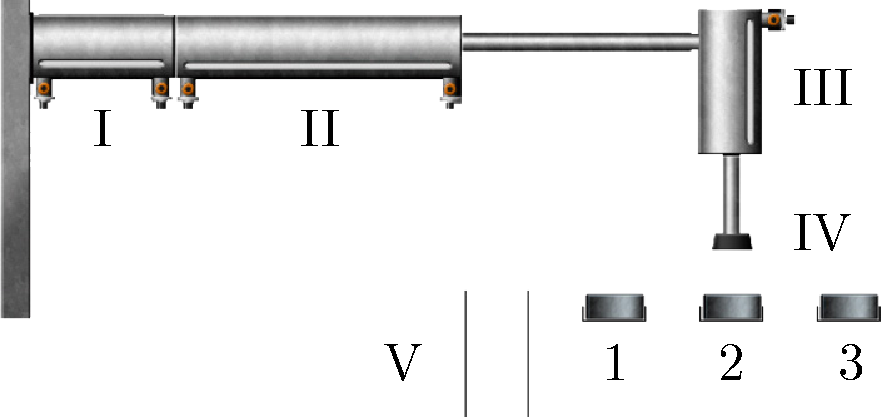
\includegraphics[width=\linewidth]{img/pnp-manipulator.pdf}
    \caption{Pick-and-Place манипулятор}%
    \label{fig:pnp-manipulator}
\end{figure}

Pick-and-Place (PnP) манипулятор, изображенный на рисунке~\ref{fig:pnp-manipulator}, состоит из двух горизонтальных пневматических цилиндров (I,~II), одного вертикального цилиндра (III) и захватывающего устройства с вакуумной присоской (IV) для подъема рабочий деталей.
Когда рабочая деталь оказывается во входном лотке (1,2,3), горизонтальные цилиндры располагают актюатор над деталью, вертикальный цилиндр опускает захватывающее устройство, который в свою очередь захватывает деталь, после чего вся система аналогичным образом приходит в движение для переноса захваченной детали в выходной лоток (V).
Данная система управления реализована в соответствии со стандартом IEC~61499 с использованием функциональных блоков в среде моделирования nxtSTUDIO~\cite{nxtstudio}.
Логический контроллер, осуществляющий управление, выполнен в виде базового функционального блока, интерфейс которого включает в себя одно входное событие \texttt{REQ} (\textit{request}), одно выходное событие \texttt{CNF} (\textit{confirmation}), а также десять входных и семь выходных переменных.
Контроллер PnP\-/манипулятора оперирует следующими входными сигналами~$\SetInputVariables$, поступающими от объекта управления \--- среды исполнения:
\begin{itemize}[nosep]
    \item \texttt{c1Home}/\texttt{c1End} \--- горизонтальный цилиндр I находится в крайнем левом/правом положении;
    \item \texttt{c2Home}/\texttt{c2End} \--- горизонтальный цилиндр II находится в крайнем левом/правом положении;
    \item \texttt{vcHome}/\texttt{vcEnd} \--- вертикальный цилиндр III находится в крайнем \mbox{верхнем}/нижнем положении;
    \item \texttt{pp1}/\texttt{pp2}/\texttt{pp3} \--- рабочая деталь находится на входном лотке 1/2/3;
    \item \texttt{vac} \--- вакуумная присоска включена.
\end{itemize}
В свою очередь контроллер PnP\-/манипулятора может посылать следующие сигналы~$\SetOutputVariables$ объекту управления:
\begin{itemize}[nosep]
    \item \texttt{c1Extend}/\texttt{c1Retract} \--- удлинить/\allowbreak{}втянуть цилиндр I;
    \item \texttt{c2Extend}/\texttt{c2Retract} \--- удлинить/\allowbreak{}втянуть цилиндр II;
    \item \texttt{vcExtend} \--- удлинить цилиндр III;
    \item \texttt{vacuum\_on}/\texttt{vacuum\_off} \--- включить/выключить ваккумную присоску.
\end{itemize}

% Данное исследование было нацелено на исследование практической применимости разработанных методов на примере синтеза описанного логического контроллера PnP\-/манипулятора.
% Процесс сбора сценариев исполнения (трассировок) для системы PnP\-/манипулятора описан в~\cite{fbCSP}.
% В данной работе были использованы наборы сценариев выполнения различных размеров: 1,~4, 10, 39 и 49 сценариев в каждом.


\subsection{Синтез минимальной конечно-автоматной модели по примерам поведения}%
\label{sub:exp-mono-pnp-scenarios-only}

Для исследования эффективности и практической применимости разработанных методов синтеза минимальных моделей по примерам поведения, производится сравнение с двухэтапным подходом из~\cite{chivilikhin-19}, где на первом этапе производится построение базовой модели, удовлетворяющей заданым сценариям выполнения, с помощью SAT-решателя, а затем охранные условия полученной модели минимизируются с помощью CSP-решателя.
Стоит отметить, что превосходство данного двухэтапного метода над другими методами, например, EFSM-tools~\cite{efsm-tools}, уже было показано в~\cite{chivilikhin-19}, поэтому сравнение происходит только с двухэтапным методом, впоследствии называемым \enquote{Two-stage}.

%% Table: Results for Extended-min-UB
\begin{table}
    \centering
    \caption{Результаты синтеза минимальной конечно-автоматной модели логического контроллера PnP\-/манипулятора по примерам поведения с помощью двухэтапного метода Two-stage~\cite{chivilikhin-19} и алгоритма $\AlgoExtendedMinUB$}%
    \label{tab:results-monolith-pnp-extminub}
    TODO
    % \subfile{tex/tab-mono-pnp-extminub-results}
\end{table}

Для синтеза минимальной конечно-автоматной модели контроллера PnP\-/манипулятора по заданным сценариям выполнения $\SetPositiveScenarios$ был применен алгоритм $\AlgoExtendedMinUB(\SetPositiveScenarios, w)$ с различными значениями параметра~$w$ \--- ширины плато для поиска локального минимума: $w = 0$ для случая, когда первое найденное решение считается финальным, $w = \infty$ для нахождения глобально-минимального решения, а также $w = 2$ для случая использования предложенной эвристики.
Результаты эксперимента представлены в таблице~\ref{tab:results-monolith-pnp-extminub}, где
$\SetPositiveScenarios$ \=== набор сценариев выполнения,
$\card{\PositiveTree}$ \=== размер дерева сценариев;
\enquote{Время, с} \--- время работы в секундах,
$\Nmin$ \--- минимальный суммарный размер охранных условий;
для метода Two\=/stage~\cite{chivilikhin-19}:
$\Cmin$ \--- минимальное число состояний,
$\Tmin$ \--- минимальное число переходов;
для метода $\AlgoExtendedMinUB$:
минимальное число состояний опущено, так как совпадает с $\Cmin$ для двухэтапного метода,
$P$ \=== максимальный размер каждого охранного условия,
$T$ \=== число переходов (не было минимизировано),
$w$ \=== критическая ширина плато для предложенной эвристики.
Результаты свидетельствуют о том, что разработанный метод $\AlgoExtendedMinUB$ способен генерировать более компактные конечные автоматны, чем двухэтапный метод, при этом значения эвристического параметра $w = 2$ достаточно для получения оптимального результата в терминах $\Nmin$.


\subsection{Синтез минимальной конечно-автоматной модели по примерам поведения и LTL-спецификации}%
\label{sub:exp-mono-pnp-with-ltl}

%% Table: LTL properties
\begin{table}[p]
    \centering
    \caption{Темпоральные свойства для системы PnP\-/манипулятора}%
    TODO
    % \label{tab:ltl-properties}
    % \begin{adjustbox}{max width=\textwidth, max height=\maxheight{1}}
    %     \subfile{tex/tab-ltl-properties}
    % \end{adjustbox}
\end{table}

Следующий эксперимент посвящен учету формальной спецификации с помощью применения индуктивного синтеза, основанного на контрпримерах.
Для использования LTL-свойств \emph{живости} (\textit{liveness}) верификация моделей с помощью NuSMV проводилась в замкнутом цикле~\cite{closed-loop} с заранее подготовленной формальной моделью объекта управления \--- PnP\-/манипулятора.
Эта модель определяет состояние объекта управления в зависимости от команд управления контроллера \--- синтезированной конечно-автоматной модели.
Набор использованых LTL-свойств представлен в таблице~\ref{tab:ltl-properties} и включает в себя как свойства безопасности \Prop{1}\==\Prop{6} (\enquote{система не окажется в нежелательном состояния}), так и свойства живости \Prop{7}\==\Prop{10} (\enquote{что-то полезное когда-нибудь произойдет}).
При этом свойства $\PropertiesConst$ зафиксированы, то есть используются во всех экспериментах, а использование свойств $\PropertiesVar$ разнится.
Стоит отметить, что эти три свойства определяют тот факт, что если рабочая деталь (1\==3) размещается на входном лотке, то она когда-нибудь будет обработана.
Однако в оригинальной системе PnP\-/манипулятора~\cite{patil-pnp} выполняется \emph{только} свойство \PropWP{1}, касающееся первой детали \--- если в первом входном лотке всегда присутствует рабочая деталь (при ее подъеме на ее месте в этот же момент появляется новая), то рабочие детали во втором и третьем входных лотках никогда не будут обработаны, что нарушает свойства живости \PropWP{2} и \PropWP{3}.
Поэтому каждое дополнительное (по отношению к $\PropertiesConst$) свойство $\PropertiesVar$ рассматривается отдельно от остальных, при этом предполагается, что рабочие детали появляются только на соответствующих входных лотках.
Для эксперимента с использованием дополнительного LTL-свойства \PropWP{2} был использован специальный набор сценариев $\SetScenarios^{(1)\prime\prime}$, состоящий из одного сценария, описывающего обработку детали во втором входном лотке.
Аналогично, для свойства $\PropWP{3}$ был использован специальный набор сценариев $\SetScenarios^{(1)\prime\prime\prime}$, состоящий из одного сценария, описывающего обработку детали в третьем входном лотке.

Проведенное экспериментальное сравнение включало в себя три метода: два разработанных метода $\AlgoCegis$ и $\AlgoCegisMin$, входящие в состав \smallcaps{fbSAT}, а также расширение метода \smallcaps{fbCSP} для учета LTL\-/спецификации, называемое впоследствии \mbox{\smallcaps{fbCSP+LTL}}~\cite{chivilikhin-18}.
Для обоих разработанных методов параметры $C^{*}$ и $P^{*}$ были предварительно оценены с помощью алгоритма $\AlgoExtendedMinUB$ с параметром $w = 2$, время работы было учтено в суммарном времени работы алгоритма CEGIS\@.
% Для обоих разработанных методов использовалось значение параметра $w = 2$, эффективность которого была показана ранее (раздел~\ref{sub:exp-mono-pnp-scenarios-only}).
% Помимо времени работы методов и значения суммарного размера охранных условий $N$, также было учтено число итераций CEGIS\@.
Дополнительно, синтезированные модели были вручную протестированы в nxtSTUDIO~\cite{nxtstudio} \--- загружены в симуляционную среду и проверены на соответствие желаемому поведению.
Результаты данного экспериментального исследования представлены в таблице~\ref{tab:results-monolith-pnp-cegis}, где
\enquote{Дополнительное LTL-свойство} \--- одно из свойств $\PropertiesVar$, использованное в дополнение к свойствам $\PropertiesConst$,
$\SetPositiveScenarios$ \=== набор использованых позитивных сценариев выполнения $\SetPositiveScenarios$,
$N_{\text{init}}$ \--- начальный минимальный суммарный размер охранных условий (для автомата, полученного с помощью алгоритма $\AlgoExtendedMinUB(\SetPositiveScenarios, w)$),
\enquote{Время, с} \--- время работы в секундах,
$P$ \=== максимальный размер охранного условия,
$N$ \=== финальный суммарный размер охранных условий (при использовании алгоритма $\AlgoCegisMin$ это значения является минимальным),
\enquote{\#iter} \--- число итераций CEGIS\@.

%% Table: Results for CEGIS
\begin{table}
    \centering
    % \captionsetup{justification=centering} % выравнивание подписи по-центру
    \caption{Результаты применения подхода CEGIS к синтезу конечно-автоматной модели логического контроллера PnP\-/манипулятора по примерам поведения и LTL\-/спецификации}%
    \label{tab:results-monolith-pnp-cegis}
    TODO
    % \subfile{tex/tab-mono-pnp-cegis-results}
\end{table}

Анализируя полученные результаты, можно заметить, что модели, найденные с помощью подхода CEGIS всегда имеют больший размер (в терминах суммарного размера охранных условий~$N$), нежели модели, построенные только по сценариям выполнения.
Это объясняется тем, что используемые сценарии выполнения не полностью покрывают рассмотренную LTL\-/спецификацию.
Поэтому алгоритм $\AlgoCegisMin$ всегда находит наименьшее решение и во всех случаях превосходит \mbox{\smallcaps{fbCSP+LTL}}~\cite{chivilikhin-18}, как по времени работы, так и по размеру моделей.
Наиболее интересным результатом является то, что $\AlgoCegisMin$ позволяет эффективно синтезировать модели по наборам сценариев $\SetScenarios^{(1)}$, $\SetScenarios^{(1)\prime\prime}$ и $\SetScenarios^{(1)\prime\prime\prime}$ \--- эти сценарии \enquote{не~покрывают} соответствующие свойства живости $\PropertiesVar$ в том смысле, что эти сценарии описывают процесс обработки только одной рабочей детали.
Существующий метод \smallcaps{fbCSP+LTL}~\cite{chivilikhin-18} не справился в этих случаях, в то время как разработанный метод $\AlgoCegisMin$ с легкостью преуспел.
Также стоит отметить, что алгоритм $\AlgoCegis$ позволяет синтезировать модели быстрее, однако не обеспечивает минимальности охранных условий.


\section{Экспериментальное исследование: SYNTCOMP}%
\label{sec:experiments-monolith-syntcomp}

%% Weird boolvec notation from the original BoSy paper
\newcommand{\myboolvec}[1]{2^{#1}}

В этом разделе описывается применение разработанных методов к задаче синтеза системы переходов (\textit{transition system})~\cite{bosy,not-bosy} по входным данным с соревнования по реактивному синтезу SYNTCOMP~\cite{syntcomp}.
Один из треков соревнования SYNTCOMP \--- трек последовательного синтеза (\textit{sequential synthesis track}) \--- посвящен задаче синтеза системы переходов по заданной LTL\-/спецификации, также известной как задача LTL-синтеза.
Существует множество различных программных средств, осуществляющих LTL-синтез, среди которых можно выделить BoSy~\cite{bosy,not-bosy} и Strix~\cite{strix}.
Стоит отметить, что среди всех доступных программных средств только BoSy ограничивает размеры (число состояний) генерируемых систем переходов, однако BoSy не минимизирует размеры охранных условий, что значительно затрудняет анализ получаемых систем человеком.
Также стоит отметить, что на текущий момент разработанное в данной работе программное средство \smallcaps{fbSAT} неприменимо в явном виде к задаче LTL-синтеза, так как для \smallcaps{fbSAT} необходимым условием является наличие некоторого множества позитивных сценариев выполнения~$\SetPositiveScenarios$.
Несмотря на это, \smallcaps{fbSAT} может быть применен для \emph{минимизации} систем переходов, генерируемых BoSy.

Формально\footnote{%
    Здесь стоит отметить, что в данном разделе для описания системы переходов используется \emph{оригинальная} нотация из~\cite{not-bosy}.
    Эта нотация может конфликтовать с другими частями данной работы \--- следует считать, что все объявления в данном разделе действуют только здесь.
    Также стоит отметить, что в оригинальной нотации для обозначения \emph{множества всех наборов значений} пропозициональных переменных используется нотация $\myboolvec{X}$, где $X$ \--- множество пропозициональных переменных, однако более корректным обозначением было бы $\boolvec{X}$.
},
\emph{система переходов} $\mathcal{T}$ это кортеж $\Tuple{ T, t_0, \Sigma = I \union O, \tau }$, где
$T$ \--- множество состояний,
$t_0 \in T$ \--- стартовое состояние,
$\Sigma$ \--- алфавит системы,
$I$ \--- множество пропозициональных переменных, управляемых окружением (\emph{входы}),
$O$ \--- множество пропозициональных переменных, управляемых системой (\emph{выходы}),
$\tau : T \times \myboolvec{I} \to \myboolvec{O} \times T$ \--- функция перехода, отображающая состояние~$t$ и входной набор $\bm{i} \in \myboolvec{I}$ в выходной набор $\bm{o} \in \myboolvec{O}$ и новое состояние~$t'$.
% $\Pair{t, \bm{i}} \mapsto \Pair{\bm{o}, t'}$
Можно заметить сходство систем переходов и конечно-автоматных моделей ECC базовых функциональных блоков.
Если система переходов обладает семантикой, схожей с семантикой автомата Мура (то есть выходы в функции перехода зависят от состояния системы), то такая система может быть смоделирована в виде ECC, а значит и синтезирована с помощью \smallcaps{fbSAT}\@.

% \begin{equation}
%     \label{eq:moore-condition}
%     \forall t \in T
%     \ldotp
%     \forall \bm{i} \neq \bm{i}' \in \myboolvec{I}
%     \ldotp
%     \bigl[
%         \tau(t, \bm{i}) = \Pair{\bm{o}, \_\,}
%         \land
%         \tau(t, \bm{i}') = \Pair{\bm{o}', \_\,}
%     \bigr]
%     \implies
%     (\bm{o} = \bm{o}')
% \end{equation}

Наборы данных (\emph{инстансы}) на соревновании SYNTCOMP представляют собой JSON-файлы с описанием интерфейса системы и набора инвариантов \--- свойств на языке LTL, которые должны выполняться в каждый момент времени работы системы.
В листинге~\ref{lst:lilydemo19-json} приведен пример инстанса \texttt{lilydemo19}, описывающего систему с семантикой автомата Мили. Данная система оперирует входами $\Set{\texttt{ec}, \texttt{ets}}$ и выходами $\Set{\texttt{fl}, \texttt{hl}}$.
% В листинге~\ref{lst:full-arbiter-3-json} приведен пример инстанса \texttt{full\_arbiter\_3}, описывающего систему с семантикой автомата Мили. Данная система оперирует входами $\Set{r_0, r_1, r_2}$ и выходами $\Set{g_0, g_1, g_2}$.
Логика работы системы описывается с помощью LTL-свойств, указанных в поле \texttt{guarantees}, а дополнительные глобальные ограничения (предположения) записаны в поле \texttt{assumptions}.

% TODO: fix listing
% \lstinputlisting[
%     float=!htb,
%     language=json,
%     % basicstyle=\small\ttfamily,
%     caption={Инстанс \texttt{lilydemo19.json}},
%     label={lst:lilydemo19-json}
% ]{data/lilydemo19.json}

%%% \lstinputlisting[
%%%     float=!htb,
%%%     language=json,
%%%     % basicstyle=\small\ttfamily,
%%%     caption={Инстанс \texttt{full\_arbiter\_3.json}},
%%%     label={lst:full-arbiter-3-json}
%%% ]{data/full_arbiter_3.json}

При выполнении данной работы был использован набор из 136 инстансов с соревнования SYNTCOMP~2018.
Для получения конечно-автоматных моделей в формате NuSMV по имеющимся LTL\-/спецификациям было использовано программное средство BoSy (input-symbolic, QBF-encoding, максимальное число состояний: 10, максимальное время работы: 1 час), в результате чего только только для 97 из 136 инстансов были получены результирующие модели.
В листинге~\ref{lst:lilydemo19-smv} приведена NuSMV модель для инстанса \texttt{lilydemo19}.
Все полученные модели были просимулированы с помощью NuSMV с целью получения случайных сценариев выполнения различных длин.
Для этого была использована команда \enquote{\texttt{simulate~-r -k~<length>}} для симуляции (\texttt{<length>} \--- число шагов симуляции) и команда \enquote{\texttt{show\_traces -a~-v}} для сохранения трассировок.
Полученные трассировки были сконвертированы в сценарии выполнения в соответствии с разделом~\ref{sec:scenarios}.

% TODO: fix listing
% \lstinputlisting[
%     float=!htb,
%     language=nusmv,
%     % basicstyle=\small\ttfamily,
%     caption={NuSMV модель для инстанса \texttt{lilydemo19}, сгенерированная BoSy},
%     label={lst:lilydemo19-smv}
% ]{data/lilydemo19.smv}

%%% \lstinputlisting[
%%%     float=!htb,
%%%     language=nusmv,
%%%     caption={NuSMV модель для инстанса \texttt{full\_arbiter\_3}, полученная с помощью BoSy},
%%%     label={lst:full-arbiter-3-smv}
%%% ]{data/full_arbiter_3.smv}

Полученные сценарии выполнения были использованы для синтеза конечно-автоматных моделей с помощью \smallcaps{fbSAT}.
На рисунке~\ref{fig:lilydemo19} представлена синтезированная модель для описанного выше инстанса \texttt{lilydemo19}.
Для синтеза было использовано пять сценариев длины 10 (\texttt{scenarios-k5-l10}), алгоритм $\AlgoExtendedMinUB(w = 0)$, время синтеза составило менее секунды.
Модель состоит из $C = 2$ состояний и $T = 4$ переходов, а охранные условия имеют суммарный размер $N = 6$.
Дополнительный этап верификации подтвердил соответствие синтезированной системы исходной LTL\-/спецификации, указанной во входном файле \texttt{lilydemo19.json}.
Как можно заметить, синтезированная модель полностью эквивалентна исходной NuSMV модели, поэтому необходимо рассмотрение более \enquote{сложного} инстанса.

%% Picture: lilydemo19 synthesized model
\begin{figure}[htb]
    % 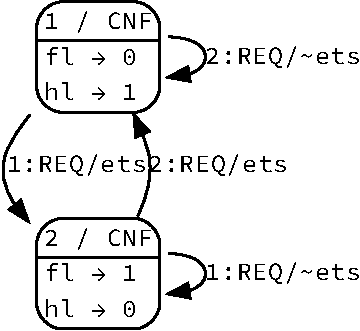
\includegraphics[max width=\textwidth]{img/lilydemo19.pdf}
    \caption{Конечно-автоматная модель для инстанса \texttt{lilydemo19}, синтезированная с помощью \smallcaps{fbSAT}}%
    \label{fig:lilydemo19}
\end{figure}

Рассмотрим инстанс \texttt{full\_arbiter\_3} \--- данная система оперирует входами $\Set{r_0, r_1, r_2}$ и выходами $\Set{g_0, g_1, g_2}$.
Полученная с помощью BoSy система переходов $\mathcal{T}_{\text{original}}$ изображена на рисунке~\ref{fig:syntcomp-bosy} и состоит из $C = 8$ состояний и $T = 28$ переходов, а суммарный размер охранных условий $N = 147$.
На этом этапе можно предположить, что полученная модель не является минимальной, а значит, возможно применение \smallcaps{fbSAT} для синтеза минимальной модели, также соответствующей исходной LTL\-/спецификации \--- для этого был использован алгоритм $\AlgoCegisMin$\@.
Стоит заметить, что для более эффективного синтеза необходимо полное покрытие состояний сценариями выполнения. Поэтому было использовано 20 сценариев, каждый длины 20 (\texttt{scenarios-k20-l20}).

Стоит отметить, что формальное определение системы переходов, данное выше, не обязывает функцию переходов $\tau$ быть детерминированной, однако \smallcaps{fbSAT} всегда генерирует детерминированные модели.
Также стоит отметить, что формальное определение системы переходов не включает в себя функцию приоритета переходов, которая присутствует в определении ECC\@.
Для того, чтобы модели, синтезируемые \smallcaps{fbSAT}, соответствовали моделям, получаемым с помощью BoSy, в \smallcaps{fbSAT} было добавлено ограничение на \enquote{дизъюнктивные переходы}\footnote{Флаг \texttt{-{}-encode-disjunctive-transitions} в \smallcaps{fbSAT}} \--- в каждом состоянии $q \in \SetStates$ для каждого входа $u \in \SetTreeInputs$ выполняется не более одного перехода.
В результате была синтезирована модель $\Automaton_{\text{deterministic}}$, изображенная на рисунке~\ref{fig:syntcomp-fbsat-deterministic}, с тем же числом состояний и переходов, что и $\mathcal{T}_{\text{original}}$, однако с меньшим суммарным размером охранных условий: $N = 105$.

Если же не использовать введенное ограничение на \enquote{дизъюнктивные переходы}, то есть использовать \smallcaps{fbSAT} в оригинальном виде, то синтезируемые модели будут детерминированными ECC (из-за функции приоритета переходов), но недетерминированными системами переходов.
В таком случае результирующая модель $\Automaton_{\text{non-deterministic}}$, изображенная на рисунке~\ref{fig:syntcomp-fbsat}, обладает наименьшим суммарным размером охранных условий: $N = 52$.

Полученные результаты показывают, что предложенный подход к явному кодированию деревьев разбора булевых формул, соответствующих охранным условиям на переходах автомата, позволяет существенно сократить суммарный размер охранных условий в автомате.
Стоит также отметить, что данный подход применим не только \emph{после} LTL-синтеза \--- возможно расширить SAT-/QBF-сведение в BoSy предложенной кодировкой для охранных условий для их минимизации непосредственно \emph{в процессе} синтеза.


\chapterconclusion

В данной главе была рассмотрена задача синтеза монолитных конечно-автоматных моделей логических контроллеров по примерам поведения и формальной спецификации.
Для решения этой задачи были разработаны методы, основанные на сведении к задаче выполнимости SAT и применении SAT-решателей.
Отдельное внимание было уделено решению задачи синтеза минимальных моделей.
Разработанные методы были реализованы в виде программного средства \smallcaps{fbSAT}~\cite{fbSAT-tool}.
Работоспособность и эффективность разработанных методов были проверены в ходе экспериментального исследования, посвященному синтезу модели логического контроллера, управляющего Pick-and-Place манипулятором.
Дополнительно, разработанные методы были применены для минимизации конечно-автоматных моделей, получаемых в ходе LTL-синтеза с помощью программного средства BoSy по исходным данным с соревнования по реактивному синтезу SYNTCOMP\@.



\FloatBarrier

\chapter{Методы оценивания декомпозиционной трудности булевых формул в применении к задачам тестирования и верификации логических схем}
\label{ch:partitionings}

% \section{Общие стратегии декомпозиции булевых формул, кодирующих задачи верификации (проверки эквивалентности) логических схем}

% % \todo{Основной вывод: нужно объединять "входы" схем, чтобы уменьшить размерность пространства поиска, а также чтобы получить меньшую дисперсию подзадач.}

% TODO: перенести этот текст в 1 главу (раздел SAT partitioning)

% Для эффективного решения сложных экземпляров SAT часто разумно использовать некоторые техники разделения исходной проблемы на более простые.
% % TODO: fix "partitioning" translation
% Естественным способом декомпозиции экземпляра SAT на подзадачи является так называемый \textit{подход к разбиению} (\textit{partitioning approach})~\cite{hyvarinen2011}.

% Рассмотрим произвольную КНФ-формулу~$C$ над множеством булевых переменных~$X$ и множество $\Pi = \{G_1, \dots, G_s\}$, где $G_i$, $i \in\nobreak \{1, \dots, s\}$, представляют собой некоторые булевы формулы над~$X$.
% Пусть $\Pi$ задает \textit{разбиение}~$C$, если выполняются следующие условия:
% \begin{enumerate}
%     \item формулы $C$ и $C \land (G_1 \lor \dots \lor G_s)$ равновыполнимы (\textit{equisatisfiable});
%     \item для всех $i \neg j \in \{1, \dots, s\}$ формула $C \land G_i \land G_j$ выполнима.
% \end{enumerate}

% Здесь и далее будем называть конъюнкцию произвольных литералов (без эквивалентных и контрарных литералов) из~$X$ как \textit{куб} над~$X$.
% Для произвольной КНФ~$C$ над переменными~$X$ простым примером разбиения является множество $\Pi = \{G_1, \dots, G_{2^r}\}$, которое состоит из всех возможных различных кубов размера~$r$ над множеством~$B$, где $|B| = r$.



% \todo{Описать различные стратегии разбиения: по переменным (входы / (не-)балансные гейты), по кубам (CnC?), по чанкам (объединение входов), по интервалам.}



В данной главе описывается общий подход к оценке трудности примеров SAT, связанных с булевыми схемами, относительно одного класса методов разбиения этих примеров на подформулы.
Такого рода оценка трудности, фактически представляет собой некоторую верхнюю границу сложности рассматриваемой формулы, выраженной в некоторых единицах, которые можно использовать для измерения времени работы полного SAT-решателя.
Также предлагаются две простые конструкции разбиения, которые показали хорошие результаты в вычислительных экспериментах.\\


% ======================================================

\section{Трудность относительно разбиения и вероятностный алгоритм её оценки}

Легко видеть, что можно связать с определенным разбиением SAT $\Pi$ и конкретным полным SAT-решателем $A$ случайную величину $\xi_{\Pi}$ так, что общее время работы $A$ на всех SAT-экземплярах из разбиения $\Pi$ может быть выражено через математическое ожидание $\xi_{\Pi}$ (которое мы обозначаем как $\E[\xi_{\Pi}]$).
Этот факт дает теоретические основания для оценки трудности относительно разбиения с помощью простого алгоритма Монте-Карло.

Рассмотрим произвольную КНФ $C$ над переменными $X$, и пусть $A$ -- полный SAT-решатель.
Пусть $\Pi = \{G_1, \dots, G_s\}$ -- произвольное разбиение $C$.
Можно рассматривать $\Pi$ как пространство элементарных событий~\cite{feller1971}, где $G_i$, $i \in \{1, \dots, s\}$ -- элементарные события.
Далее, пусть $p_i$ -- положительные числа, связанные с каждым $G_i$ таким образом, что $\sum_{i=1}^{s} p_i = 1$.
Установим $p_i = 1/s$ для каждого $i \in \{1, \dots, s\}$, задав таким образом равномерное распределение на $\Pi$.
Затем определим случайную величину $\xi_{\Pi} \colon \Pi \to \Real^{+}$ следующим образом:
\begin{equation}
    \label{f-star}
    \xi_{\Pi}(G \in \Pi) = t_A(G \land C),
\end{equation}
где $t_A(G \land C)$ обозначает время, затраченное $A$ на определение выполнимости формулы $G \land C$.

\begin{definition}\label{def:hardness-wrt-part}
    Трудность $C$ относительно алгоритма $A$ и разбиения $\Pi$ определяется как значение:
    \begin{equation}\label{eq:hardness-wrt-part}
        \mu_{A,\Pi}(C) = \sum_{i=1}^s t_A(G_i \land C)
    \end{equation}
\end{definition}

\begin{theorem}\label{thm:hardness-wrt-partitioning}
    Справедливо соотношение: $\mu_{A,\Pi}(C) = s \cdot \E[\xi_{\Pi}]$.
\end{theorem}

\begin{proof}%[Набросок доказательства]
    В контексте сказанного выше, имеем вероятностное пространство, где $\Pi = \{G_1,...,G_s\}$ \--- пространство элементарных событий, а $\xi_{\Pi}$ -- определенная на нем случайная величина.
    Пусть $\fun{Spec}(\xi_{\Pi}) = \{\xi_1, \dots, \xi_r\}$ ($r \leq s$) -- спектр $\xi_{\Pi}$, где $\xi_k \in \Real^{+}$, $k \in \{1, \dots, r\}$.
    Обозначим через $\#\xi_k$ число элементарных событий в $\Pi$, для которых случайная величина $\xi_{\Pi}$ принимает значение $\xi_k$.
    Тогда вероятность события $\{\xi_\Pi = \xi_k\}$ равна $p_k = \#\xi_k / s$, и $\xi_{\Pi}$ имеет закон распределения $P(\xi_{\Pi}) = \{p_1, \dots, p_k\}$ (поскольку выполняются все аксиомы Колмогорова~\cite{feller1971}).
    Таким образом:
    \[
        \sum_{i=1}^{s} t_A(G_i \land C)
            = \sum_{k=1}^{r} \#\xi_k \cdot \xi_k
            = s \cdot \sum_{k=1}^{r} \frac{\#\xi_k}{s} \cdot \xi_k
            = s \cdot \E[\xi_{\Pi}]
        \qedhere
    \]
\end{proof}

Используя Теорему~\ref{thm:hardness-wrt-partitioning}, можно оценить $\mu_{A,\Pi}(C)$ с помощью метода Монте-Карло~\cite{metropolis1949}.
Сначала проведем $N$ независимых вероятностных экспериментов, где каждый эксперимент включает выбор $G \in \Pi$ с учетом вероятностного распределения $P = \{p_1, \dots, p_s\}$, с $p_i = 1/s$, $i \in \{1, \dots, s\}$.
Затем вычислим выборочное среднее $\xi_{\Pi}$ как $\hat{\mu} = \frac{1}{N} \sum_{j=1}^N \xi^j$, где $\xi^j$ -- значение $\xi_{\Pi}$, наблюдаемое в $j$-ом эксперименте.
Наконец, оценим $\mu_{A,\Pi}(C)$ как $\widetilde{\mu}_{A,\Pi} = s \cdot \hat{\mu}$.

Будем говорить, что $\widetilde{\mu}_{A,\Pi}(C)$ является $(\varepsilon,\delta)$-приближением~\cite{karp1989} для $\mu_{A,\Pi}(C)$, если выполняется следующее неравенство (вариация условия~\eqref{eq:cheb}):
\begin{equation}\label{eq:cheb2}
    \Pr \bigl\{
        \left| \mu_{A,\Pi}(C) - \widetilde{\mu}_{A,\Pi}(C) \right|
        \leq \varepsilon \cdot \mu_{A,\Pi}(C)
    \bigr\} \geq 1 - \delta.
\end{equation}
% Здесь $|\cdot|$ обозначает модуль, а $\Pr\{\cdot\}$ обозначает вероятность события.
Как следует из неравенства Чебышева, неравенство \eqref{eq:cheb2} выполняется для всех $N \geq \frac{\fun{Var}(\xi_{\Pi}(C))}{\varepsilon^2 \cdot \delta \cdot E[\xi_{\Pi}]^2}$, где $\xi_{\Pi}$ определена относительно \eqref{f-star}.
Однако на практике $\fun{Var}(\xi_{\Pi}(C))$ может быть очень большим, и использование малых значений $N$ может привести к недостаточной точности оценки $\mu_{A,\Pi}(C)$.
Эта проблема возникает в таких методах разбиения, как стандартная техника Cube-and-Conquer, а также схема разбиения из~\cite{CP2021}.
В следующем разделе мы представим две конструкции построения разбиений, которые позволяют уменьшить дисперсию $\fun{Var}(\xi_{\Pi})$ и, следовательно, улучшить точность оценки $\mu_{A,\Pi}(C)$.



\section{Два новых метода разбиения SAT для CircuitSAT}

В данном подразделе мы представляем два метода для построения разбиений SAT, нацеленных, главным образом, на проблемы из области CircuitSAT.
 Соответствующие конструкции могут быть применены как к LEC, так и к задачам обращения криптографических функций. Ниже приведено описание для LEC.

Рассмотрим проблему LEC для двух булевых схем $S_f$, $S_h$, задающих функции $f,h:\{0,1\}^n\rightarrow{0,1}^m$.
Определим первую конструкцию следующим образом:
\begin{construction}\label{con1}
    Рассмотрим множество переменных $\Xin = \{x_1, \dots, x_n\}$, связанных с входами схем $S_f, S_h, S_{f \glue h}$.
    Затем выберем целое число~$k$ такое, что $1 < k < n$ и разделим~$\Xin$ на~$q = \lceil n / k \rceil$ попарно непересекающихся множеств~$X^j$, где $j \in \{1, \dots, q\}$.
    Если $n$ делится на~$k$, то каждое множество~$X^j$ содержит $k$~переменных.
    В противном случае разделим~$\Xin$ на $q-1$~множества $X^1, \dots, X^{q-1}$ по $k$ переменных каждое и множество~$X^q$ размером~$r$, так что $n = k \cdot \lfloor \frac{n}{k} \rfloor + r$, где $r \in \{1, \dots, k-1\}$.
    % \lipicsEnd
\end{construction}

Рассмотрим произвольную булеву функцию $\lambda \colon \{0,1\}^l \to \{0,1\}$, где~$l \in \Natural^{+}$, и предположим, что $\lambda$~не зафиксирована.
Пусть~$\neg\lambda \colon \{0,1\}^l \to \{0,1\}$ обозначает отрицание~$\lambda$.
С каждым~$X^j$, $j \in \{1, \dots, q\}$, свяжем две КНФ $\phi_1^j$~и~$\phi_2^j$, которые определяют функции $\lambda^j \colon \{0,1\}^{|X^j|} \to \{0,1\}$ и $\neg\lambda^j \colon \{0,1\}^{|X^j|} \to \{0,1\}$ соответственно.
% Следующий факт справедлив.

\begin{theorem}\label{thm:partitioning-input-decomposition}
    Пусть $\phi^j$ обозначает обе формулы $\phi^j_1$~и~$\phi^j_2$.
    Множество~$\Pi$ всех $2^{\lceil n/k \rceil}$ возможных формул вида $\phi^1 \land \dots \land \phi^{\lceil n/k \rceil}$ формирует SAT-разбиение формулы~\eqref{eq:miter-cnf}.
\end{theorem}

\begin{proof}
    Сначала докажем, что формула $C_{f\glue h}$ имеет ровно $2^n$ выполняющих наборов.
    Действительно, рассмотрим множество $X^{in} = \{x_1,\ldots,x_n\}$ и пусть $\alpha=(\alpha_1,\ldots,\alpha_n)$ -- произвольное назначение переменных из $X^{in}$.
    Затем рассмотрим формулу $\Phi(X,\alpha) = x_1^{\alpha_1} \land \ldots \land x_n^{\alpha_n} \land C_{f\glue h}$ над множеством переменных $X$.
    Из~Леммы~\ref{lem1} следует, что применение UP к~$\Phi(X,\alpha)$ приведет к выводу значений всех переменных из этой КНФ без конфликтов.
    Для каждого $\alpha \in \{0,1\}^n$ построим такое назначение переменных из~$X$ и скажем, что это назначение генерируется соответствующим~$\alpha$.
    Обозначим построенное множество назначений над~$X$ через~$\Lambda(X)$.
    Легко видеть, что все назначения из~$\Lambda(X)$ различны.
    Далее, рассмотрим множество переменных $\tilde{X} = X \setminus X^{in}$.
    С каждым назначением $\lambda \in \Lambda(X)$ свяжем часть~$\lambda$, содержащую назначения переменных из~$\tilde{X}$.
    Обозначим построенное множество назначений как $\Lambda(\tilde{X})$.
    Пусть $\gamma\in\{0,1\}^{|\tilde{X}|}$ -- произвольное назначение переменных из $\tilde{X}$ такое, что $\gamma\notin \Lambda(\tilde{X})$.
    Очевидно, что подстановка $\gamma$ в $C_{f\glue h}$ приводит к тому, что результирующая КНФ $C_{f\glue h}[\gamma/\tilde{X}]$ является невыполнимой, поскольку для любого $\alpha = (\alpha_1,\dots,\alpha_n)$ применение UP к формуле $x_1^{\alpha_1} \land \dots \land x_n^{\alpha_n} \land C_{f \glue h}[\gamma/\tilde{X}]$ приведет к конфликту.
    Таким образом, любой выполняющий набор $C_{f \glue h}$ -- это назначение, сгенерированное некоторым $\alpha\in\{0,1\}^{|X^{in}|}$, и различные назначения из $\{0,1\}^{|X^{in}|}$ порождают различные выполняющие наборы~$C_{f \glue h}$.
    Таким образом, у формулы $C_{f\glue h}$ ровно $2^n$ выполняющих наборов.
    С другой стороны, нетрудно видеть, что любое $\alpha \in \{0,1\}^{|X^{in}|}$ выполняет ровно одну формулу $G_i$, $i \in \{1,\dots,2^{\lceil n/k \rceil}\}$ описанного выше вида.
    Таким образом, формулы $C_{f\glue h}$ и $(G_1 \lor \dots G_{2^{\lceil n/k \rceil}})$ имеют одинаковые выполняющие наборы, и, следовательно, формулы $C_{f\glue h}\land C(M)$ и $(G_1 \lor \ldots G_{2^{\lceil n/k \rceil}}) \land C_{f\glue h} \land C(M)$ равновыполнимы.
\end{proof}

Важный вопрос состоит в том, как выбрать функции $\lambda^j$ и $\neg\lambda^j$ таким образом, чтобы гарантировать малую дисперсию $\fun{Var}(\xi_\Pi)$ для разбиения SAT описанного выше типа? Здравый смысл подсказывает, что  имеет смысл использовать \textit{сбалансированнаые} булевы функции, т.е. такие функции, которые принимают значение~1 на $2^{l-1}$ входных словах, в качестве функции $\lambda \colon \{0,1\}^l \to \{0,1\}$.
Очевидно, что отрицание сбалансированной функции тоже является сбалансированной функцией. Хорошим примером такого рода функции для $l > 1$ является функция, задаваемая формулой $x_1 \xor \dots \xor x_l$.

Далее проведем несколько неформальный анализ свойств Конструкции~\ref{con1}, и используем его результаты в качестве основы для Конструкции~\ref{con2}, которая показала налучшие результаты среди всех рассмотренных методов в экспериментах с некоторыми чрезвычайно сложными примерами LEC в виде SAT.
Рассмотрим функцию~\eqref{eq:f-glue-h} и шаблонную КНФ~$C_{f \glue h}$.
Многочисленные эксперименты показывают, что даже когда SAT для $C_{f \glue h} \land C(\mathcal{M})$ является чрезвычайно сложной, SAT для $C_{f \glue h}$ остается простой: любой CDCL SAT-решатель, получив на вход $C_{f \glue h}$ и не имея никакой дополнительной информации о структуре схемы, способен найти выполняющий набор для $C_{f \glue h}$.
Этот набор можно рассматривать как сертификат выполнимости для $C_{f \glue h}$.
Как мы отмечали выше, всего для КНФ $C_{f\Delta h}$ существует $2^n$ таких сертификатов.
Таким образом, доказательство невыполнимости $C_{f \glue h} \land C(\mathcal{M})$ можно рассматривать как процесс, который опровергает все эти сертификаты.
Более того, если функции~$\lambda^j$ сбалансированы для каждого $j \in \{1, \dots, \lceil n/k \rceil\}$, то каждая формула вида $\phi^1 \land \dots \land \phi^{\lceil n/k \rceil} \land C_{f \glue h}$ имеет $2^{n-\lceil n/k \rceil}$ выполняющих наборов, которые также являются сертификатами удовлетворимости.
Таким образом, можно сделать два предположения:
\begin{enumerate}
    \item Алгоритму~$A$ намного легче доказать невыполнимость формулы $\phi^1 \land \dots \land \phi^{\lceil n/k \rceil} \land C_{f \glue h} \land C(\mathcal{M})$, потому что ему необходимо опровергнуть $2^{n-\lceil n/k \rceil}$ сертификатов вместо~$2^n$.
    \item Для сбалансированных функций $\lambda^{j}$, $j \in \{1, \dots, \lceil n/k \rceil\}$, все $2^{\lceil n/k \rceil}$ различных формул вида $\phi^1 \land \dots \land \phi^{\lceil n/k \rceil} \land C_{f \glue h} \land C(\mathcal{M})$ должны быть более или менее схожи по времени работы алгоритма~$A$ на них, т.е. разбиение~$\Pi$, заданное Конструкцией~\ref{con1}, должно иметь малую дисперсию $\fun{Var}(\xi_{\Pi})$.
\end{enumerate}

Хотя представленные аргументы лишены строго формального доказательства, на практике их выводы экспериментально подтверждаются.
Ниже опишем еще одну конструкцию, при разработке которой были учтены указанные выше свойства.

Основная идея описанной ниже конструкции заключается в том, чтобы рассмотреть произвольное назначение переменных из $\Xin =\{x_1,\ldots,x_n\}$ в качестве коэффициентов двоичного представления числа из $N_{0}^{n} = \{0,1,\ldots,2^n-1\}$.
Таким образом, существует взаимно однозначное отображение вида $\{0,1\}^n \to N_{0}^{n}$.
Для произвольных $a,b \in N_{0}^{n}$ назовем множество чисел $\Set{ q \in N_{0}^{n} \given a \leq q \leq b }$ \textit{интервалом} и обозначим такой интервал как~$[a,b]$.
Рассмотрим множество булевых векторов из $\{0,1\}^n$, которые являются двоичными представлениями чисел из~$[a,b]$, как множество решений следующего целочисленного неравенства, предполагая, что $x_i$, $i \in \{1,\dots,n\}$ принимают значения из $\{0,1\}$:
\begin{equation}\label{eq-ineq}
    a \leq x_n + 2\cdot x_{n-1} + \dots + 2^{n-1} \cdot x_1 < b
\end{equation}
Скажем, что множество~$\mathcal{R}^n$, образованное интервалами описанного вида, является \textit{полной системой интервалов}, если никакие два интервала из~$\mathcal{R}^n$ не пересекаются и любое число из $N_{0}^{n}$ принадлежит какому-либо интервалу в~$\mathcal{R}^n$.
Это означает, что любая полная система интервалов порождает разбиение $\{0,1\}^n$ на непересекающиеся подмножества, образованные решениями соответствующих неравенств \eqref{eq-ineq}.

\begin{construction}\label{con2}
    Пусть $\mathcal{R}^n$ \--- полная система интервалов.
    С произвольным $I \in \mathcal{R}^n$, $I = [a,b]$, ассоциируем неравенство вида~\eqref{eq-ineq} и CNF~$C_I$, полученное путем кодирования\eqref{eq-ineq} в SAT с использованием соответствующих техник, например, представленных в~\cite{een2006}.
    Определим $\Pi = \{C_I\}_{I \in \mathcal{R}^n}$.
\end{construction}

\begin{theorem}\label{thm3}
    Множество $\Pi = \{C_I\}_{I\in \mathcal{R}^n}$, полученное с использованием Конструкции~\ref{con2}, формирует SAT-разбиение формулы $C_{f\Delta h} \land C(\mathcal{M})$.
\end{theorem}

\begin{proof}%[Набросок доказательства]
    Аналогично доказательству Теоремы~\ref{thm:partitioning-input-decomposition}, используем Лемму~\ref{lem1}, чтобы показать, что любое назначение, удовлетворяющее $C_{f \glue h}$, также удовлетворяет ровно одну формулу вида $G_i \land C_{f \glue h}$, $i \in\nobreak \{1, \dots, s\}$.
    Следовательно, мы можем заключить, что $C_{f \glue h} \land C(\mathcal{M})$ и $C_{f \glue h} \land C(\mathcal{M}) \land (G_1 \lor\nobreak \dots \lor\nobreak G_s)$ равновыполнимы.
    С другой стороны, ясно, что любая КНФ вида $G_i \land G_j$, $i \neq j$, $i,j \in \{1, \dots, s\}$, невыполнима, что означает, что $\Pi = \{G_1, \dots, G_s\}$ является SAT-разбиением формулы $C_{f \glue h} \land C(\mathcal{M})$.
\end{proof}

Заметим, что в случае, когда $\mathcal{R}^{n}$ формируется интервалами равного размера~$2^{l}$, где $1 \leq l < n$, то можно указать любой интервал $I \in \mathcal{R}^{n}$ без использования кодировок из~\cite{een2006}.
Действительно, в этом конкретном случае интервал с номером $k \in \{ 1,\dots,2^{n - l} \}$ состоит из чисел вида $(k - 1) \cdot \nobreak 2^{l} +\nobreak j$, где $j = 0, \dots, 2^{l}-1$.
Следовательно, этот интервал можно указать с помощью двоичного вектора $\lambda_{l + 1} \dots \lambda_{n}$, где $\lambda_{q}$, $q \in \{l+1, \dots, n\}$, являются коэффициентами из $\{0,1\}$ в двоичном представлении числа ${ (k - 1) \cdot 2^{l} }$ из $n$~бит.

Заметим, что описанный подход не применим к интервалам произвольного вида.
В самом деле, рассмотрим небольшой пример: для $n=6$ вектор $(010111)$ указывает на число $23$, а вектор $(101000)$ соответствует числу $40$.
Тогда, не существует числа $i\in\{1,\ldots,6\}$ такого, что $x_i$ принимает одно и то же значение во всех числах из интервала $[23,40]\cap N_0$.
Поэтому в общем случае необходимо применять техники, такие как например, описанные в~\cite{een2006}, для кодирования интервалов вида~\eqref{eq-ineq} в SAT.


% \section{Экспериментальное исследование}
% \section{Вероятностный и статистический анализ свойств предложенных разбиений}

% \todo{Вычислительные эксперименты и их результаты}
% \todo{Multipliers, Sorters, Cryptography}
% \todo{Статистические оценки, результаты из IEEE, доверительные интервалы, обоснование мощности выборки}

\section{Вычислительные эксперименты}
\label{sec:experiments}

Все эксперименты, представленные в данном разделе, были проведены на кластере Университета ИТМО, каждый узел которого оснащен двумя 18-ядерными процессорами Intel Xeon E5-2695~v4 и 128~ГБ оперативной памяти.
В качестве SAT-решателя были использованы Kissat\footnote{\url{https://github.com/arminbiere/kissat}} (версия 3.0.0) и CaDiCaL\footnote{\url{https://github.com/arminbiere/cadical}} (версия 1.9.5) из-за их высокой производительности, широких возможностей по настройке и программному взаимодействию через API.
Это было согласовано даже при использовании подхода CnC с инкрементальными решателями (включая те, которые интегрированы в репозиторий CnC и последнюю версию CaDiCaL).
Kissat выделялся при решении кубов на всех тестовых наборах и решателях.

Основным вопросом, который мы изучали в вычислительных экспериментах, была точность оценок сложности относительно разбиения (в смысле формулы~\eqref{def:hardness-wrt-part}).
Ситуации, когда сложность относительно разбиения меньше или близка к времени работы последовательного решателя на исходной задаче, являются особенно интересными, потому что в таких случаях соответствующие разбиения позволяют не только точно оценить время решения задачи (в отличие от случая последовательного решения), но и обеспечивают более эффективную стратегию решения соответствующего экземпляра LEC.

% Все дополнительные материалы к настоящей статье доступны онлайн\footnote{\url{https://github.com/Lipen/FMCAD-2023-Supplementary}}.


\subsection{Тестовые данные}

Мы рассматриваем два класса тестовых наборов (бенчмарков).
Первый класс состоит из (невыполнимых) экземпляров задачи LEC для схем, представляющих алгоритмы умножения, такие как
\enquote{умножение столбиком}, \enquote{дерево Уоллеса}~\cite{cormen1990}, \enquote{алгоритм Карацубы}~\cite{knuth-vol2} и \enquote{умножитель Дадда}~\cite{dadda1965}.
Эти экземпляры обозначаются как \instance{AvB}{k}, где \Instance{A} и \Instance{B} означают алгоритмы умножения, а $k$ \=== количество бит в умножаемых числах.
Например, \instance{CvK}{16} представляет собой экземпляр LEC для проверки эквивалентности умножения двух 16-битных чисел (\texttt{16x16} умножитель) методом столбика и алгоритмом Карацубы.
Известно, что такого рода тестыи крайне сложны для современных SAT-решателей~\cite{kaufmann2019,CP2021}.

Второй класс состоит из нескольких (выполнимых) экземпляров, связанных с алгебраическим криптоанализом~\cite{bard2009}, а именно, SAT-кодировок атаки поиска прообраза для хеш-функции MD4 с уменьшенным числом раундов.
Эта проблема была недавно решена в~\cite{zaikin2022} с использованием подхода Cube and Conquer.
Набор тестовых примеров на основе MD4 служит для того, чтобы показать, что предложенная техника применима к (1)~выполнимым тестам (2)~тестам не из области LEC.


\subsection{Эксперименты по оценке декомпозиционной сложности}

В первом наборе экспериментов оценим сложность экземпляров LEC для умножителей относительно предложенных разбиений SAT, где мы разбиваем множество входов~$\Xin$ на непересекающиеся подмножества, называемые \emph{чанками}, в соответствии с Конструкцией~\ref{con1}.
Мы рассматриваем следующие виды функций~$\lambda^j$:
\begin{itemize}
    \item \Part{2-XOR}: $\lambda^1 = x_1 \xor x_2$, \Part{3-XOR}: $\lambda^1 = x_1 \xor x_2 \xor x_3$, \textit{и т.д.};
    \item \Part{2-DIS}: $\lambda^1 = x_1 \lor x_2$;
    \item \Part{3-MAJ}: $\lambda^1 = \fun{majority}(x_1, x_2, x_3)$, где $\fun{majority}(a, b, c) = (a \land b) \lor (a \land c) \lor (b \land c)$;
\end{itemize}
Функции $\lambda^j$ для $j > 1$ определены на соответствующих непересекающихся чанках входов, например, $\lambda^2 = x_4 \xor x_5 \xor x_6$ для \Part{3-XOR}.
Во всех случаях формулы, соответствующие $\lambda_1^j = \lambda^j$ и $\lambda_2^j = \neg\lambda^j$, были закодированы в~КНФ.

Аналогично, для разбиений SAT, построенных в соответствии с Конструкцией~\ref{con2}, мы используем обозначение \Part{INT-s}, где $s$~обозначает количество интервалов, например, \Part{INT-65536} соответствует разбиению на \np{65536} подзадач.

Чтобы обеспечить достоверность и актуальность наших результатов, среди всех составленных бенчмарков были выбраны только те экземпляры, которые представляют практический интерес, то есть те, которые не решаются за несколько секунд, но при этом могут быть решены за разумное время.
Для тестовых наборов алгоритмов сортировки были выбраны экземпляры, которые кодируют LEC для $k = 9$ и~$l = 4$.
Среди умножителей были выбраны экземпляры двух разных уровней сложности (умножители \texttt{12x12} и \texttt{16x16}, например, \instance{CvK}{12} или \instance{KvW}{16}) для демонстрации гибкости нашего подхода в решении задач с различной сложностью.
Для каждого выбранного тестового примера были построены соответствующие разбиения и были решены \textbf{все} подзадачи, чтобы вычислить истинные значения математического ожидания~$\E[\xi_\Pi]$ и дисперсии~$\fun{Var}(\xi_\Pi)$.

Кроме того, были рассмотрены разбиения, построенные с использованием техники Cube and Conquer (CnC).
Для этой цели были построены кубы с помощью \texttt{march\_cu}\footnote{\url{https://github.com/marijnheule/CnC}}.
В частности, были подобраны значения опций \texttt{-d <depth>} и \texttt{-n <number>} таким образом, чтобы размеры полученных разбиений были аналогичны разбиениям, построенным с помощью методов, предложенных в данной работе.
Для некоторых \enquote{простых} экземпляров также был запущен \texttt{march\_cu} с параметрами по умолчанию, которые могут рассматриваться как базовый уровень в этом экспериментальном исследовании.
Отметим, что для некоторых \enquote{более сложных} тестов \texttt{march\_cu} в режиме по умолчанию не смог выдать результаты (т.е. набор кубов) за разумное время (24~часа), что привело к пропуску этих экспериментов.
Затем все полученные кубы были независимо решены параллельно.
Далее в этом документе будем обозначать разбиения, сгенерированные в идеологии CnC, как \Part{CnC-d*}, \Part{CnC-n*} и \Part{CnC-default}.

\begin{table}[!ht]
    \centering
    \caption{Экспериментальные результаты для SAT-разбиений для задачи проверки эквивалентности (LEC) умножителей}
    \label{tab:results-partitionings-best}
    \subfile{tex/tab-parts-best}
\end{table}

\begin{figure}[!ht]
    \centering
    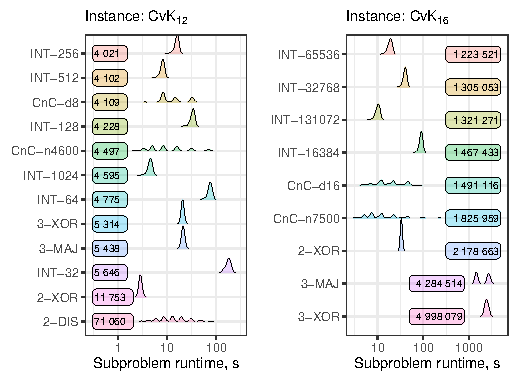
\includegraphics[scale=1.5]{plot_merged-ridges_CvK-12-CvK-16_all-ID-INT-CnC_kissat.pdf}
    \caption{Распределения времени выполнения SAT-решателя на подзадачах в различных разбиениях экземпляров LEC \instance{CvK}{12} (слева) и \instance{CvK}{16} (справа). Цифры рядом с графиками плотности указывают общее время выполнения (в секундах), и все разбиения упорядочены по общему времени (наименьшее время сверху)}
    \label{fig:ridges}
\end{figure}

Результаты экспериментов кратко представлены на Рисунке \ref{fig:ridges}~и в Таблице~\ref{tab:results-partitionings-best}.
В~частности, Рисунок~\ref{fig:ridges} содержит
подробные результаты для \textit{всех} обсуждаемых типов разбиений на двух выбранных экземплярах (\instance{CvK}{12} и \instance{CvK}{16}).
В то же время, Таблица~\ref{tab:results-partitionings-best} представляет \emph{лучшие} разбиения для остальных экземпляров.
Для каждого разбиения приводится среднее и стандартное отклонение (\enquote{Avg~$\pm$~sd}), диапазон времени выполнения подзадач (\enquote{Min\,--\,max}) и общее  время (CPU Time), необходимое для решения всех подзадач.
Таблица также включает строки \enquote{Sequential} для представления базовой производительности последовательного решателя SAT.

Графики на Рисунке~\ref{fig:ridges} визуализируют дисперсию времени выполнения SAT-решателя при использовании рассматриваемых схем разбиения.
Для конструкций \ref{con1}~и~\ref{con2} (разбиения \Part{2-XOR} и \Part{INT}, соотвественно) время работы SAT-решателя имеет относительно низкую дисперсию, что указывает на то, что мы можем точно оценить необходимое общее время выполнения, используя относительно небольшой объем выборки.
Напротив, для Cube and Conquer и разбиений \Part{2-DIS} дисперсия значительно больше из-за неравномерного распределения сложности подзадач.
Для последнего это можно объяснить несбалансированностью функции $\lambda = a \lor b$, используемой в \Part{2-DIS}.
Эти результаты подчеркивают важность выбора подходящих схем разбиения для достижения построения точной оценки общего времени выполнения.

Экспериментальные результаты показывают, что оценка для разбиения не всегда согласуется с временем работы последовательного решателя на исходной задаче.
При этом, интересно, что наши результаты показывают, что общее время, необходимое для решения всех подзадач для умножителей, существенно меньше времени, необходимого для последовательного решения соответствующих тестовых примеров.
В частности, для 16-битных умножителей однопоточный решатель не смог завершить работу даже после 10 дней, в то время как все подзадачи в разбиении были решены за разумное и \emph{предсказуемое} время, соответствующее оценке.
Для \enquote{Sequential} строки в таблицах следует уточнить, что решатель работал на одном ядре, в то время как все остальные эксперименты вычислялись параллельно, и представленное общее время CPU является суммой времени работы на всех подзадачах.

\begin{figure*}[!ht]
    % Note: total text width is 43pc, each of 4 subfigures should have width=1.7in
    \centering
    \subfloat[][\instance{CvK}{16}, \Part{2-XOR} / \np{65536}]{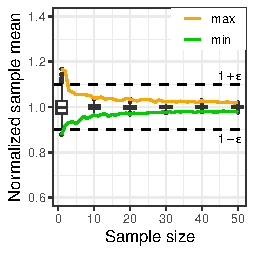
\includegraphics{plot_samples-min-max-boxplots_CvK-16_2-XOR_kissat.pdf}}
    \hfill
    \subfloat[][\instance{CvK}{16}, \Part{INT} / \np{65536}]{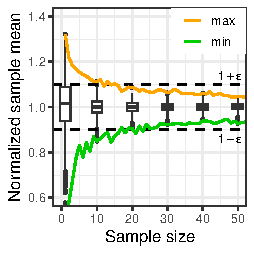
\includegraphics{plot_samples-min-max-boxplots_CvK-16_INT-65536_kissat.pdf}}
    \hfill
    \subfloat[][\instance{CvK}{16}, \Part{CnC-d16} / \np{65536}]{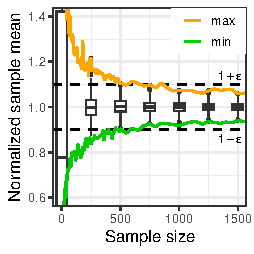
\includegraphics{plot_samples-min-max-boxplots_CvK-16_CnC-d16_kissat.pdf}}
    \hfill
    \subfloat[][\instance{MD4}{40}, \Part{INT} / \np{110000}]{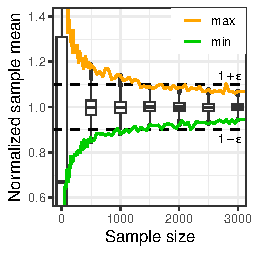
\includegraphics{plot_samples-min-max-boxplots_MD4-40_INT-110000_kissat.pdf}}
    \caption{Распределения выборочных средних для различных размеров выборок~$N$ для экземпляра LEC \instance{CvK}{16} и задачи нахождения прообраза MD4 \instance{MD4}{40}}
    \label{fig:min-max-CvK-16-kissat}
\end{figure*}

В контексте всего сказанного выше, одной из основных проблем является точность полученных оценок~$\E[\xi_\Pi]$, так как
дисперсия~$\fun{Var}(\xi_\Pi)$ оказывает отрицательное влияние на точность.
Однако результаты в Таблице~\ref{tab:results-partitionings-best} показывают, что предложенные методы SAT-разбиения дают очень низкую дисперсию на рассматриваемых бенчмарках.
Это является значительным преимуществом предложенного метода, так как он позволяет использовать небольшую случайную выборку для получения надежной оценки~$\E[\xi_\Pi]$.
Для демонстрации этого проведем дополнительный анализ полученных результатов.

Для различных значений~$N$ сгенерируем $P = 1000$ случайных выборок размера~$N$ и вычислим средние значения выборок $(\hat{\xi}^1, \dots, \hat{\xi}^P)$, где каждое $\hat{\xi}^r = \frac{1}{N} \bigsumnolim{j=1}^{N} \xi_j^r$.
Также вычислим среднее значение средних значений выборок $\Xi(N) = \frac{1}{P} \sum_{r=1}^{P} \hat{\xi}^r$ и минимальные и максимальные значения среди~$\hat{\xi}$, которые мы обозначаем как $M_*(N)$~и~$M^*(N)$, соответственно.
Далее все значения нормализуем путем деления их на~$\E[\xi_\Pi]$.
Распределения нормализованных средних значений для различных размеров выборки показаны на Рисунке~\ref{fig:min-max-CvK-16-kissat}, где горизонтальная ось представляет размер случайной выборки~$N$.
Здесь мы рассматриваем экземпляр пример, кодирующий LEC задачу для умножителей~\instance{CvK}{16} и два различных разбиения: \Part{INT-65536} (предложенное разбиение на \np{65536}~интервалов) и \Part{CnC-d16} (Cube and Conquer, построенное при помощи \texttt{march\_cu -d 16}).
На графиках показаны нормализованные линии для минимальных и максимальных значений, представленных как $M_*(N) / \E[\xi_\Pi]$ (зеленая линия, внизу) и $M^*(N) / \E[\xi_\Pi]$ (оранжевая линия, сверху), соответственно.
Результаты показывают, что выборочное среднее~$\hat{\xi}$ является надежной оценкой~$\E[\xi_\Pi]$, даже когда $N$ гораздо меньше общего размера разбиения.
Например, размер выборки~$N \approx 30$ из общего числа \np{65536}подзадач для разбиения \Part{INT-65536} для теста \instance{CvK}{16} достаточен для получения оценки в пределах 10\%\=/интервала $\E[\xi_\Pi]$.
Наоборот, достаточный размер выборки для разбиений CnC обычно значительно больше, в частности, для \Part{CnC-d16} (которое также имеет размер \np{65536}), он составляет как минимум $N \approx 1000$.

\subsection{Эксперименты по поиску прообразов MD4}
\label{sub:experiments-md4}

Чтобы показать, что предложенные конструкции применимы и к другим сложным экземплярам CircuitSAT, помимо невыполнимых LEC-бенчмарков, мы применили их к задаче поиска прообразов для хэш-функции MD4 с уменьшенным числом раундов.
Эта проблема интересна тем, что лучшие известные результаты для нее были получены с помощью метода Cube-and-Conquer со специализированной стратегией поиска параметров CnC.

В наших экспериментах мы взяли две CNF (md4\_40steps\-\_11.30\=/32Dobb\_one\-\_constr\-\_one\_hash, обозначаемую как $\instance{MD4}{40}$, и md4\_43steps\_12Dobb\-\_one\-\_constr\-\_one\_hash, обозначаемую как $\instance{MD4}{43}$) из репозитория\footnote{\url{https://github.com/olegzaikin/MD4-CnC}}, представленного в~\cite{zaikin2022}.
Эти CNF соответствуют двум не слишком легким и не слишком трудным случаям криптоанализа.
Используя Конструкцию~\ref{con2}, мы провели серию оценок времени выполнения, варьируя количество интервалов, и использовали наилучшие найденные параметры разбиения для полного решения обеих задач.
Как и в~\cite{zaikin2022}, были решены все подзадачи, то есть процесс не останавливался как только был найден выполняющий набор.

\begin{table}[!tb]
    \centering
    \caption{Экспериментальные результаты для разбиений экземпляров MD4}
    \label{tab:results-md4}
    \subfile{tex/tab-md4}
\end{table}

Результаты этой серии экспериментов обобщены в Таблице~\ref{tab:results-md4}.
Они сравниваются с результатами, опубликованными в~\cite{zaikin2022}, обозначенными как \Part{CnC} (время выполнения последних было представлено для 12~ядер CPU, поэтому мы масштабировали их для одного ядра CPU).
Стоит отметить, что в статье~\cite{zaikin2022} также использовалась стратегия, адаптированная к данной конкретной задаче, для поиска оптимальных параметров разложения CnC, хотя время нахождения этих параметров не включено в Таблицу~\ref{tab:results-md4}, а также использовалась вычислительная платформа с более быстрыми ядрами CPU.
Тем не менее, используя наш простой метод,  удалось решить рассмотренные задачи за время, сравнимое с временем в~\cite{zaikin2022}.
В~Таблице~\ref{tab:results-md4} строки, помеченные \enquote{(est.)}, соответствуют оценкам времени работы, построенным по случайным выборкам размером~$N = 1000$, а строки, помеченные \enquote{(full)}, соответствуют решению всех подзадач из построенного разбиения.
Оцененное время работы также отмечено звездочкой в колонке \enquote{Time}.
Из распределения выборочных средних для $\instance{MD4}{40}$, представленного на правом графике на Рисунке~\ref{fig:min-max-CvK-16-kissat}, видно, что выбранного значения размера выборки ($N = 1000$) достаточно для построения точных оценок времени работы.
Расхождения между реальным временем решения и расчетным временем в Таблице~\ref{tab:results-md4} еще раз показывают, что предложенные конструкции дают небольшую дисперсию в трудности подзадач.


\chapterconclusion

% TODO

В этой главе были представлены результаты экспериментального исследования, которые показывают, что предложенные методы разбиения задачи SAT позволяют получить точные оценки время работы SAT-решателя.

\chapter{Методы декомпозиции примеров задачи SAT, кодирующих синтез и верификацию ДУС, основанные на вероятностных лазейках}
\label{ch:backdoors}

...


%%% Заключение
\chapter*{ЗАКЛЮЧЕНИЕ}
\addcontentsline{toc}{chapter}{Заключение}

В данной диссертационной работе была достигнута поставленная цель \--- повышение эффективности полных алгоритмов решения задачи булевой выполнимости (SAT) применительно к синтезу и верификации моделей автоматных программ. Разработаны оригинальные методы и техники декомпозиции булевых формул, что позволило существенно сократить время работы алгоритмов.

В ходе исследования созданы новые алгоритмы кодирования задач синтеза конечных автоматов и булевых схем, отличающиеся возможностью использования произвольных элементарных гейтов и явным кодированием структуры охранных условий в виде деревьев разбора формул. Предложены методы декомпозиции булевых формул, обеспечивающие точную оценку декомпозиционной трудности задач благодаря низкой дисперсии времени решения подзадач. Масштабные вычислительные эксперименты подтвердили практическую значимость предложенных методов. Разработанные алгоритмы успешно применены для решения сложных примеров синтеза и верификации моделей автоматных программ, включая конечные автоматы и логические схемы.

Созданная программная библиотека \texttt{kotlin-satlib} предоставляет унифицированный интерфейс для работы с современными SAT-решателями, облегчая процесс моделирования и решения задач синтеза и верификации. Библиотека включает модули для интеграции с SAT-решателей через технологию JNI, упрощения записи ограничений с использованием преобразований Цейтина, манипуляции переменными с конечными доменами и работы с многомерными массивами SAT-переменных.

Результаты исследования демонстрируют, что предложенные методы и алгоритмы могут быть эффективно интегрированы в существующие системы синтеза и верификации моделей автоматных программ.
Они также могут быть адаптированы для решения других задач, связанных с булевой выполнимостью, что открывает возможности для дальнейших исследований и разработок.

Перспективы дальнейшего развития темы включают углубленное исследование методов декомпозиции булевых формул, разработку новых алгоритмов для специфических классов задач и расширение функциональности программной библиотеки для поддержки большего числа SAT-решателей и разнообразных типов задач. Таким образом, проделанная работа вносит значительный вклад в область синтеза и верификации моделей автоматных программ, предлагая более эффективные и гибкие инструменты для решения сложных задач.


%%% Список сокращений и условных обозначений
% % Если оч надо это автоматизировать, то смотри здесь
% https://www.overleaf.com/learn/latex/Nomenclatures
%\printnomenclature[3.5cm] % Значение ширины столбца с обозначениями стоит подбирать вручную


%%% Словарь терминов:
% \chapter*{Словарь терминов}             % Заголовок
\addcontentsline{toc}{chapter}{Словарь терминов}  % Добавляем его в оглавление

\textbf{TeX} : Cистема компьютерной вёрстки, разработанная американским профессором информатики Дональдом Кнутом

\textbf{панграмма} : Короткий текст, использующий все или почти все буквы алфавита


%%% Списки таблиц и изображений
% \clearpage
\ifdefmacro{\microtypesetup}{\microtypesetup{protrusion=false}}{} % не рекомендуется применять пакет микротипографики к автоматически генерируемым спискам
\listoffigures  % Список изображений

%%% Список таблиц %%%
% (ГОСТ Р 7.0.11-2011, 5.3.10)
\clearpage
\listoftables   % Список таблиц
\ifdefmacro{\microtypesetup}{\microtypesetup{protrusion=true}}{}
\newpage


%%% Список литературы
% https://tex.stackexchange.com/a/202797
\AtNextBibliography{\setcounter{citenum}{0}}
\printbibliography


%%% Благодарности
% \chapter*{Благодарности}
\addcontentsline{toc}{chapter}{Благодарности}


% Подсчёт количества глав
\setcounter{totalchapter}{\value{chapter}}

% Настройки для приложений
\appendix
% Оформление заголовков приложений ближе к ГОСТ:
\setlength{\midchapskip}{20pt}
\renewcommand*{\afterchapternum}{\par\nobreak\vskip \midchapskip}
\renewcommand\thechapter{\Asbuk{chapter}} % чтобы приложения русскими буквами нумеровались

%%% Приложения, в т.ч. все публикации в PDF:
\chapter{Результаты апробации методов на экземпляре \texttt{full\_arbiter\_3} с соревнования SYNTCOMP}%
\label{app:syntcomp}

\begin{figure}[!h]
    \centering
    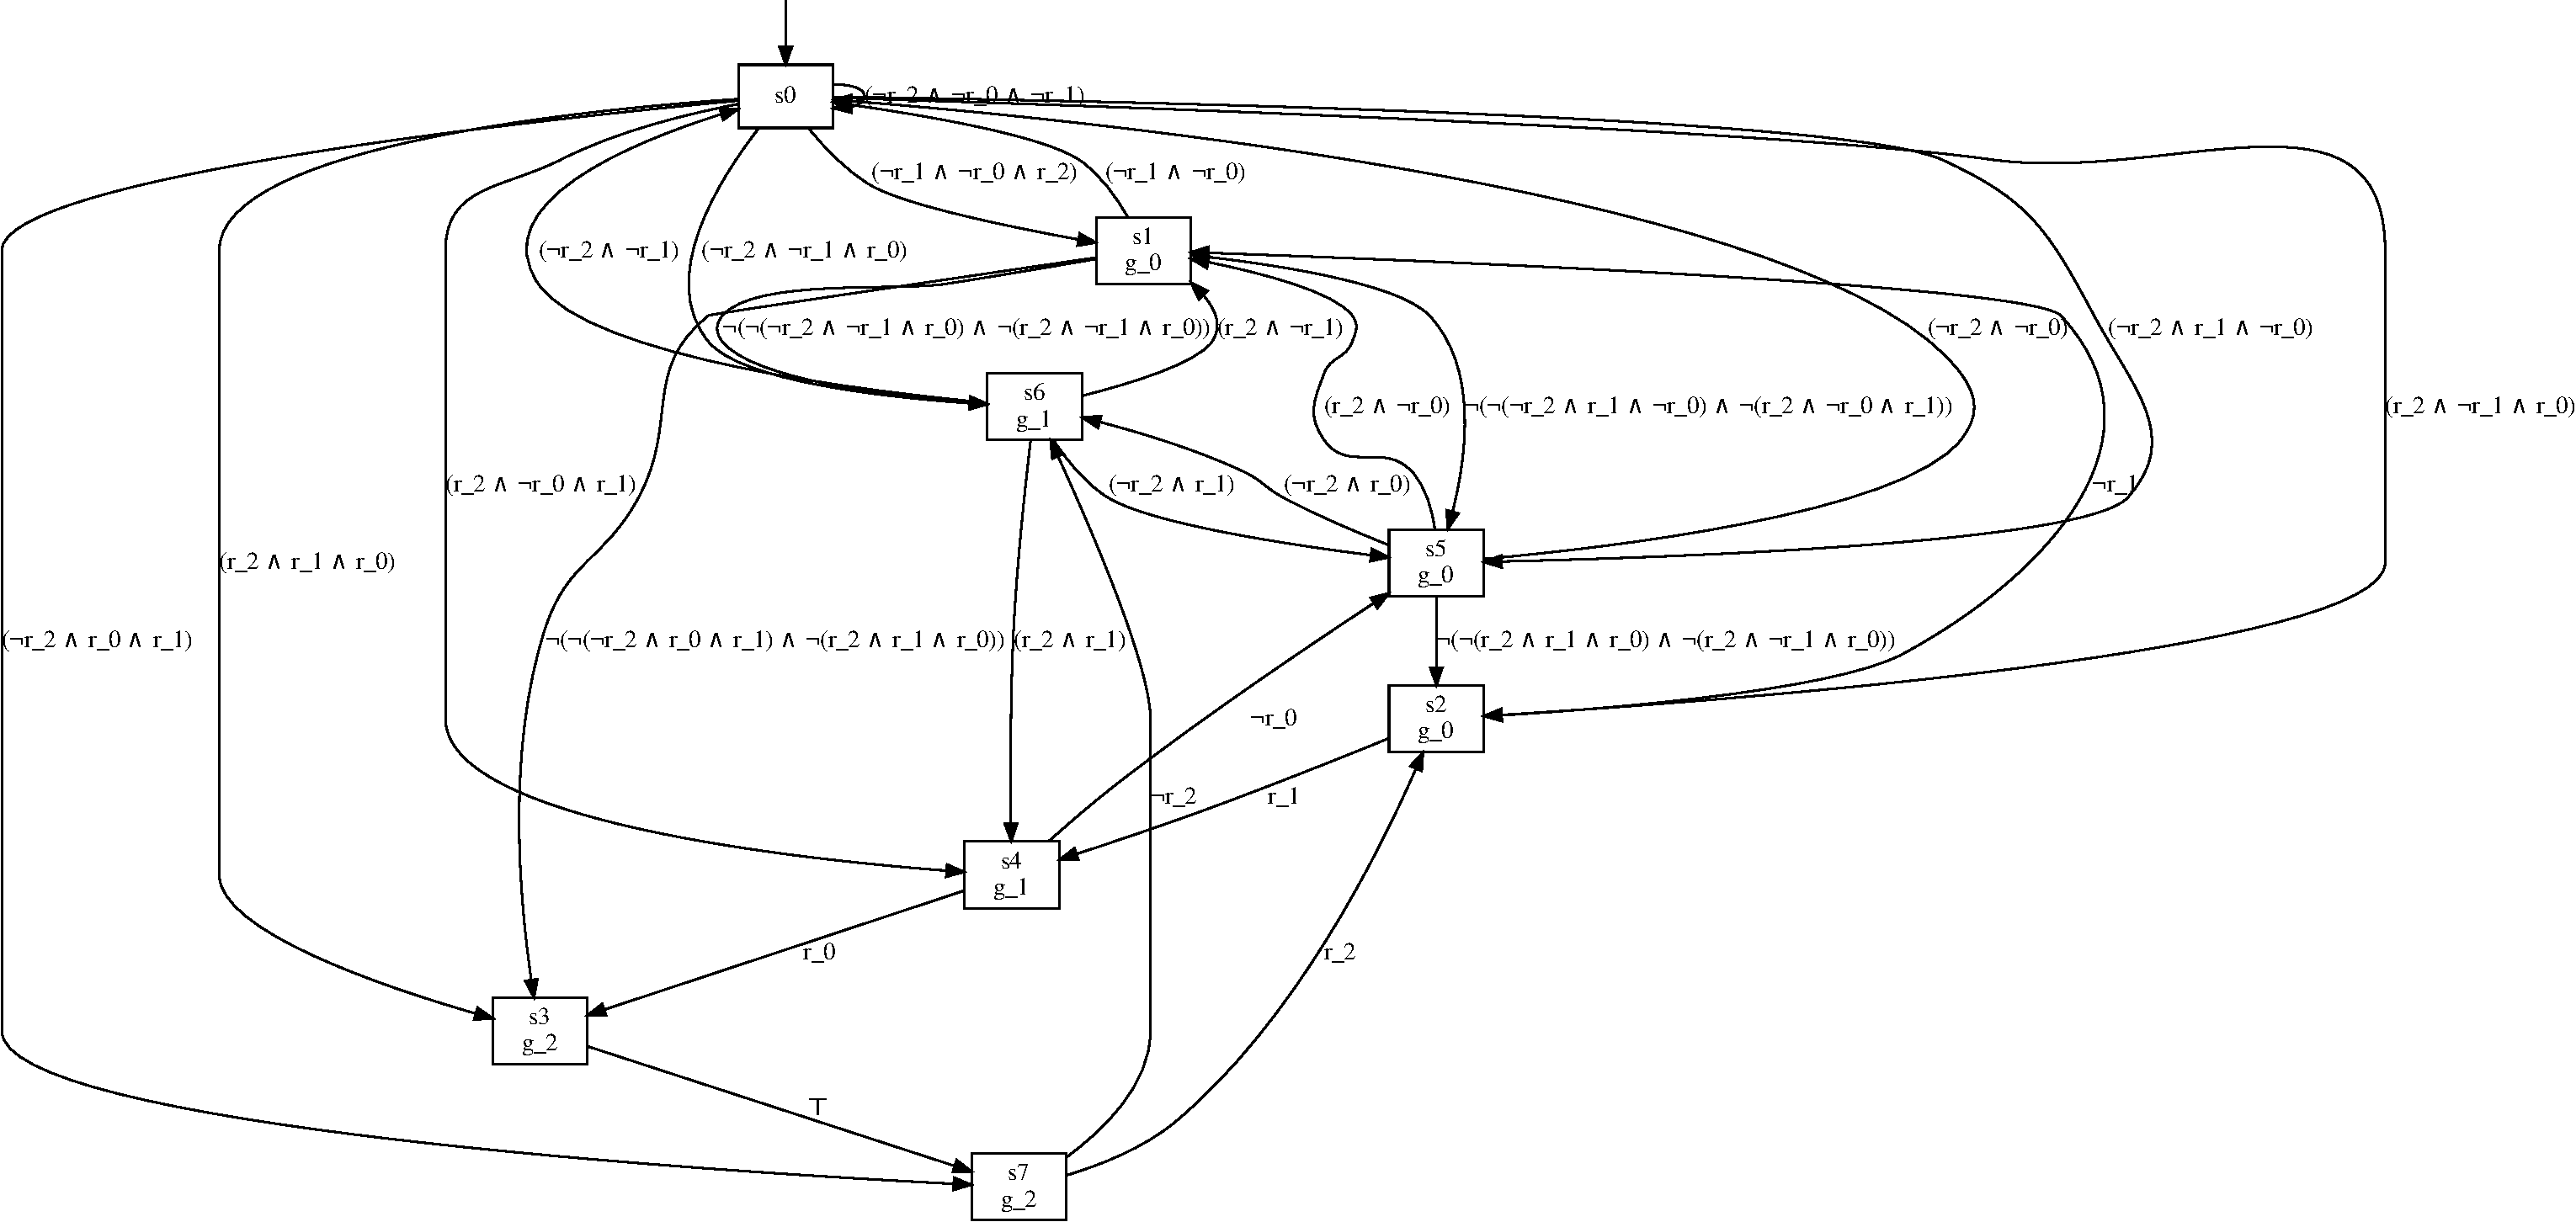
\includegraphics[rotate=90, width=\textwidth, max height=\maxheight{3}-100pt]{images/syntcomp-bosy.pdf}
    \caption{Система переходов $\mathcal{T}_{\text{original}}$, полученная с помощью BoSy для инстанса \texttt{full\_arbiter\_3}: ${C = 8}$ состояний, ${T = 28}$ переходов, суммарный размер охранных условий ${N = 147}$}%
    \label{fig:syntcomp-bosy}
\end{figure}

\begin{figure}[p]
    \centering
    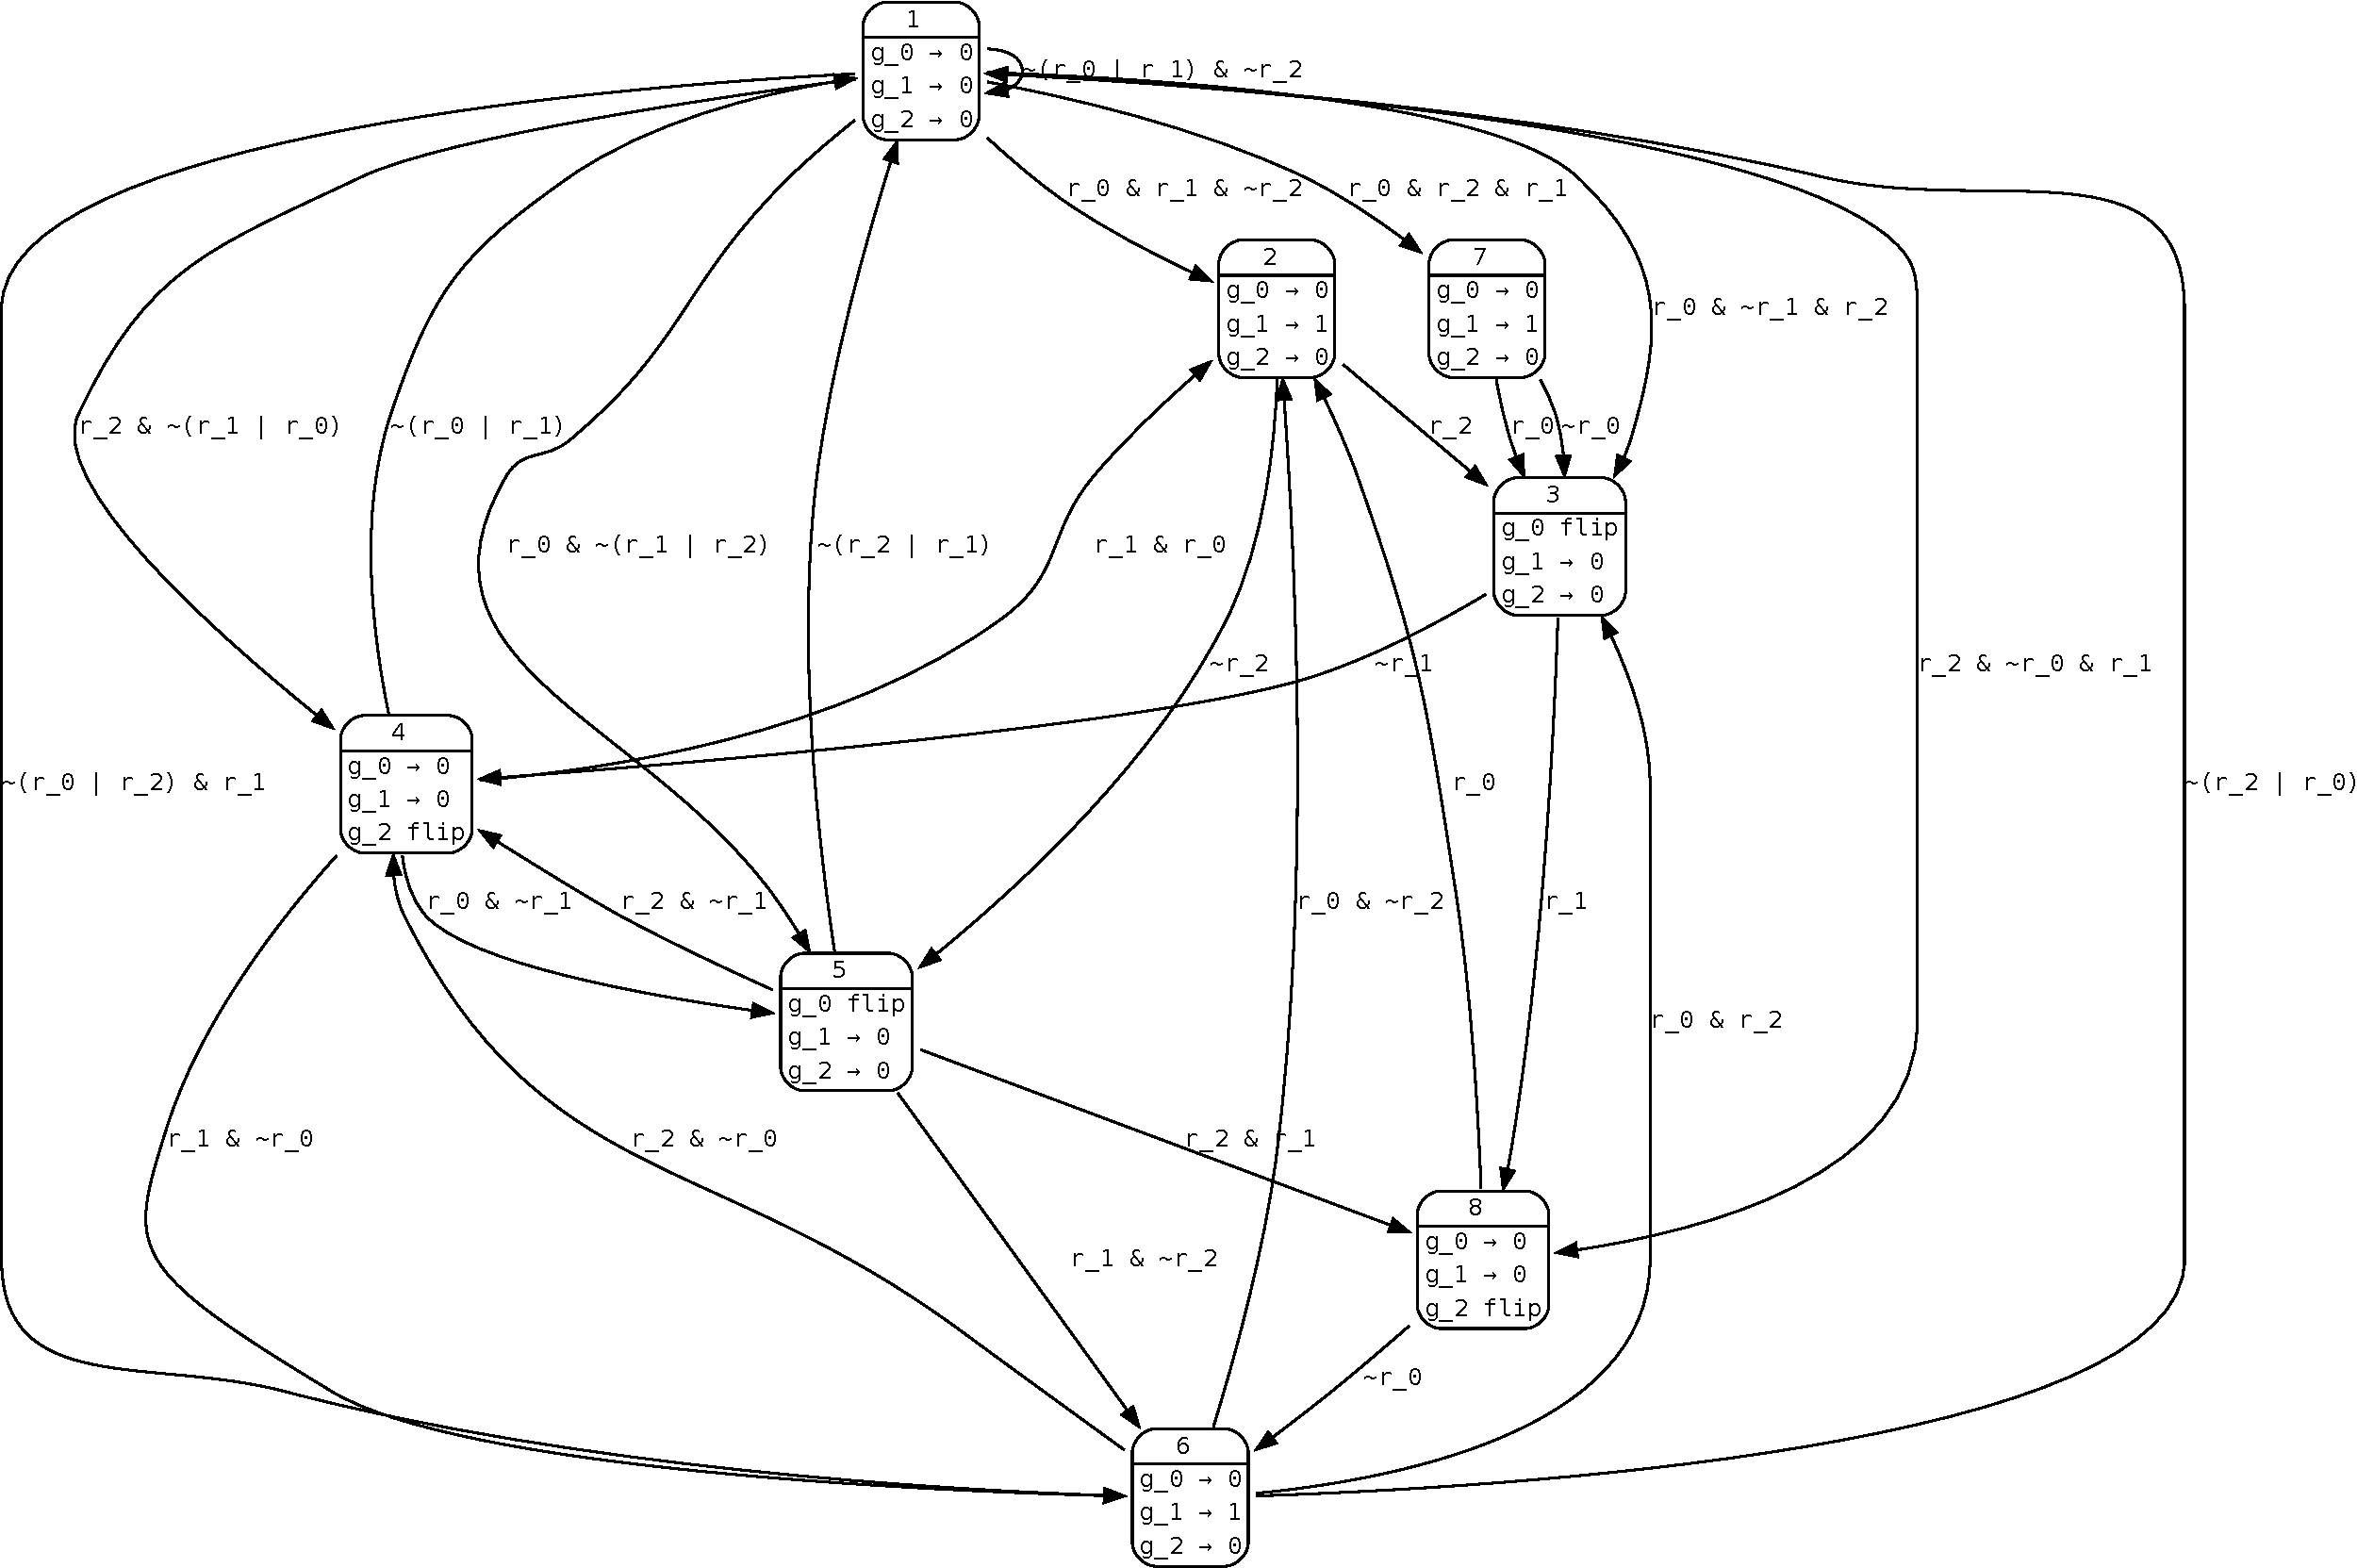
\includegraphics[rotate=90, width=\textwidth, max height=\maxheight{3}]{images/syntcomp-fbsat-deterministic.pdf}
    \caption{Детерминированная минимизированная система переходов $\Automaton_{\text{deterministic}}$, полученная с помощью \smallcaps{fbSAT}, с меньшим суммарными размером охранных условий:~${N = 105}$}%
    \label{fig:syntcomp-fbsat-deterministic}
\end{figure}

\begin{figure}[p]
    \centering
    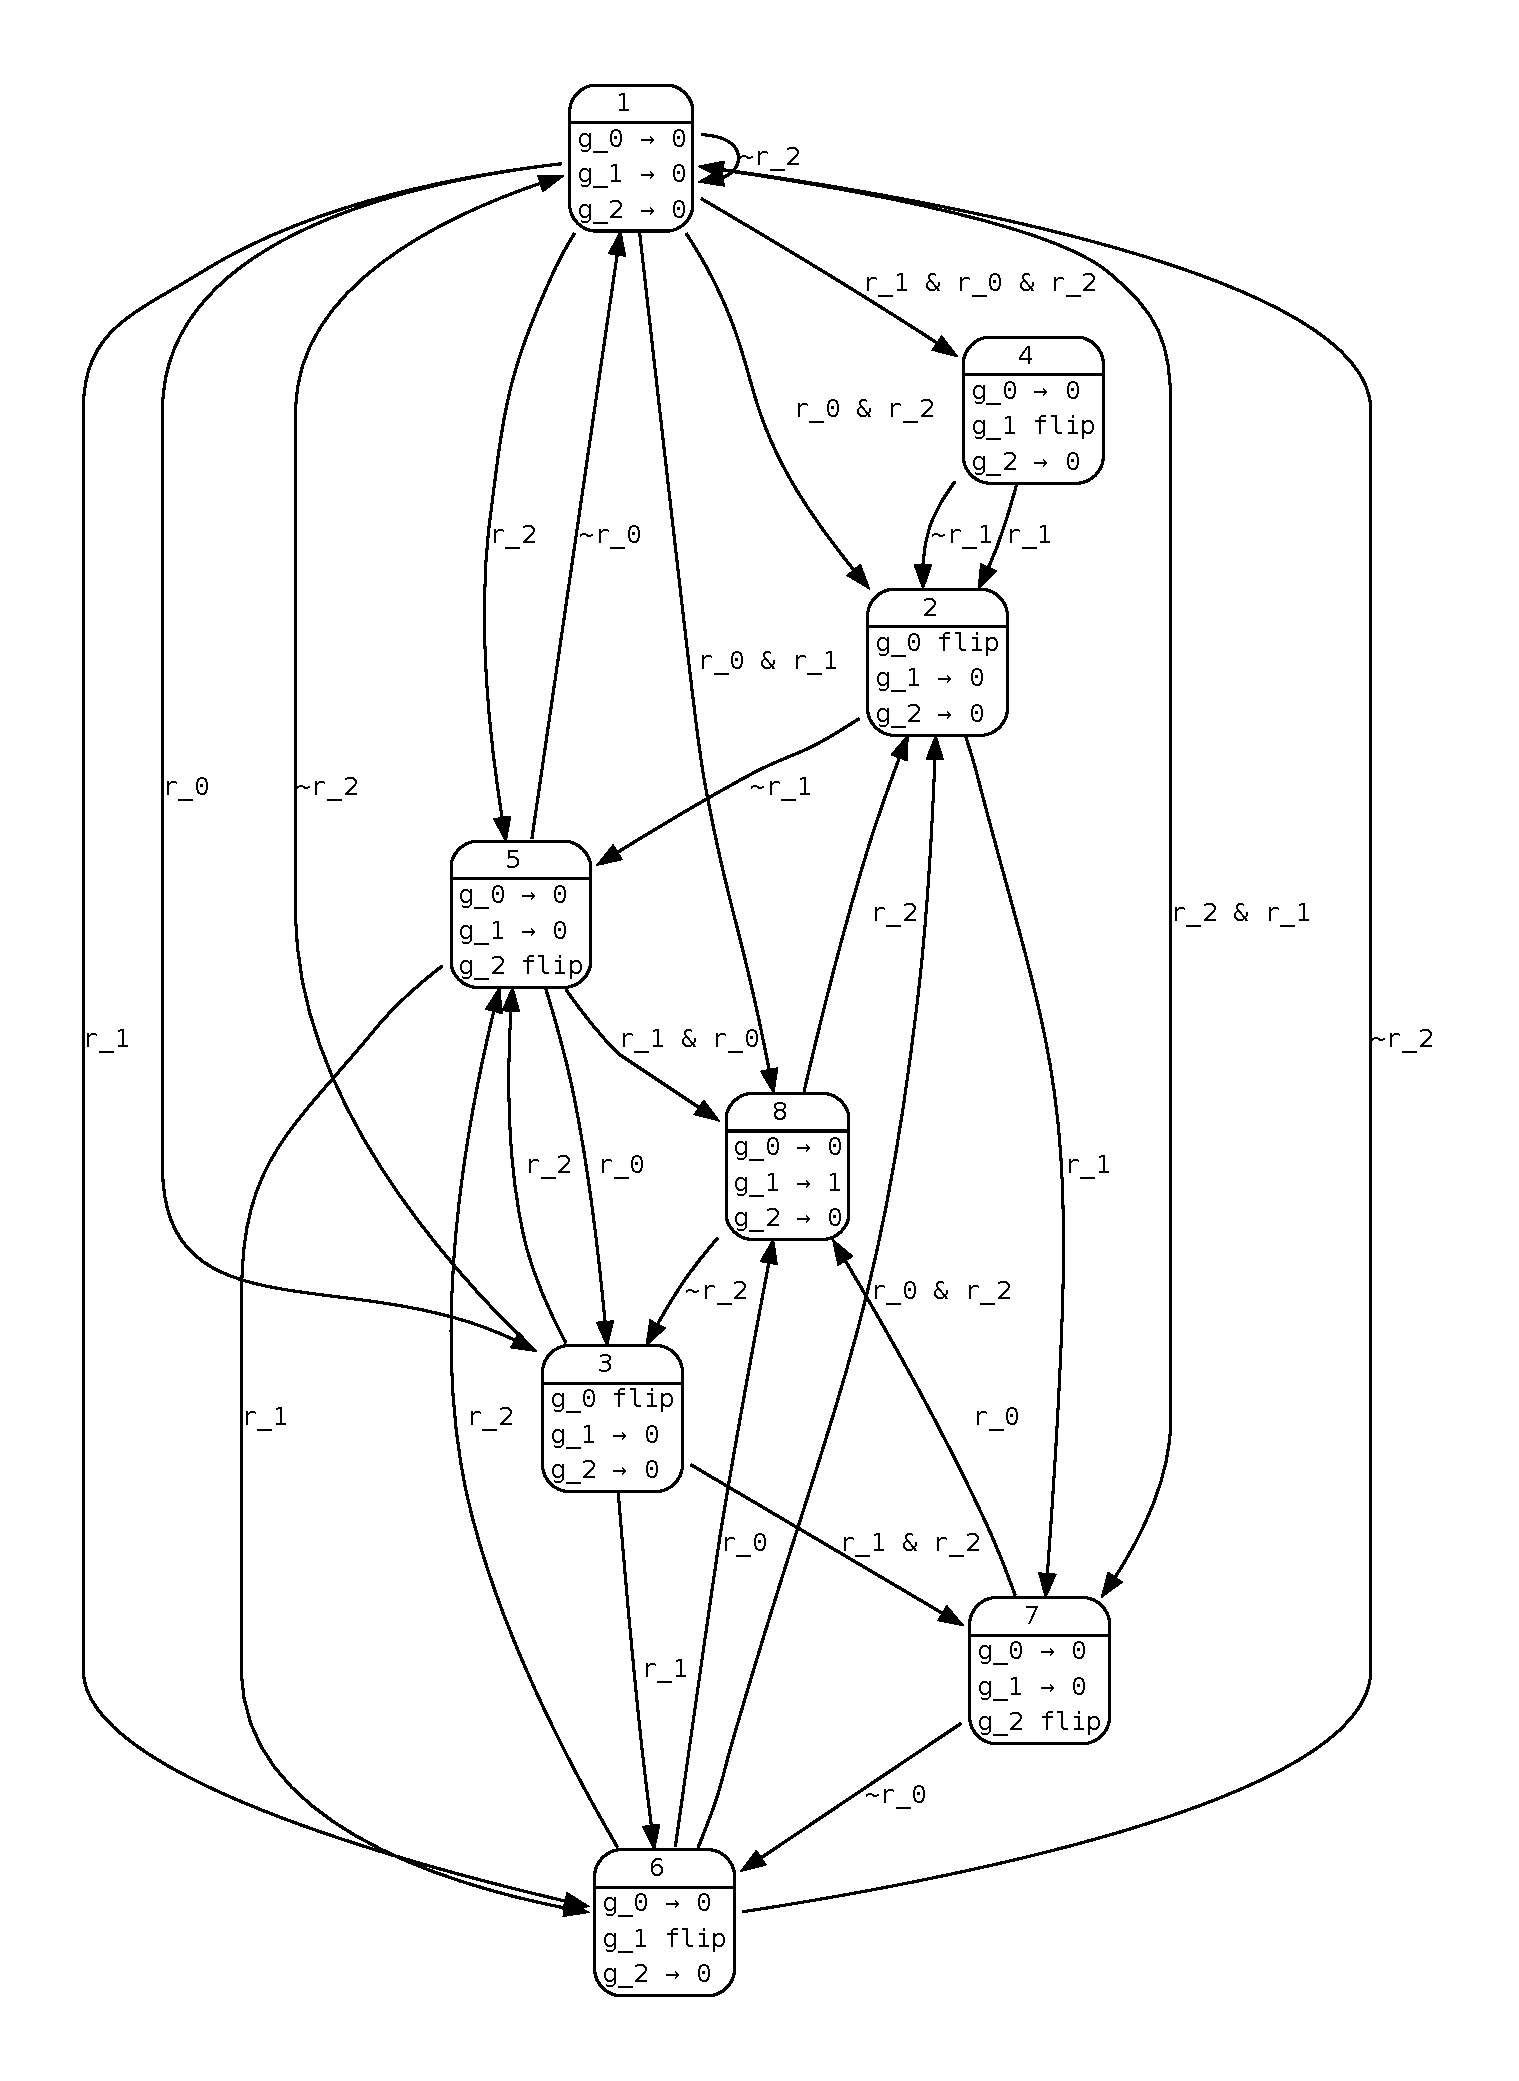
\includegraphics[width=\textwidth, max height=\maxheight{3}]{images/syntcomp-fbsat.pdf}
    \caption{Минимальная недетерминированная система переходов $\Automaton_{\text{non-deterministic}}$, полученная с помощью \smallcaps{fbSAT}, с ещё меньшим суммарным размером охранных условий:~${N = 52}$}%
    \label{fig:syntcomp-fbsat}
\end{figure}


\iffalse
\chapter{Основные публикации автора по теме диссертации}
\label{app:publications}

\newcommand{\mypublication}[2][-]{% [<pages>]{<path>}
    \includepdf[
        pages={#1},
        pagecommand={},  % to include global numbering
        scale=0.9,  % to leave space for the global page numbers
        frame, % (optional)
    ]{#2}
}

\begin{refsection}[biblio/own.bib]
\nocite{
    chivilikhin2020,%%% PLC
    chukharev2020,%%%%% CEGIS
    chukharev2020b,%%%% BF
    chukharev2022,%%%%% fbSAT
    semenov2022,%%%%%%% LEC
    andreev2024%%%%%%%% IMP
}
\printbibliography[
    keyword=own,
    % title={Список всех публикаций автора по теме диссертации},
    % heading=subbibliography,
    heading=none,
    resetnumbers=true
]
\end{refsection}

% \begin{enumerate}[beginpenalty=10000, left=0pt]
%     \item D.~Chivilikhin, S.~Patil, K.~Chukharev, A.~Cordonnier, and V.~Vyatkin, ``Automatic state machine reconstruction from legacy PLC using data collection and SAT solver'', \textit{IEEE Transactions on Industrial Informatics}, vol.~16, pp.~\np{7821}--\np{7831}, 2020.
%     \item K.~Chukharev, D.~Suvorov, D.~Chivilikhin, and V. Vyatkin, “SAT-based counterexample- guided inductive synthesis of distributed controllers”, \textit{IEEE Access}, vol.~8, pp.~\np{207485}--\np{207498}, 2020.
%     \item К.~Чухарев, <<Применение инкрементальных SAT-решателей для решения NP-трудных задач на примере задачи синтеза минимальных булевых формул>>, \textit{Научно-технический вестник информационных технологий, механики и оптики}, т.~20, №~6(130), с.~841--847, 2020.
%     \item K.~Chukharev and D.~Chivilikhin, ``fbSAT: Automatic inference of minimal finite-state
%     models of function blocks using SAT solver'', \textit{IEEE Access}, vol.~10, pp.~\np{131592}--\np{131610},
%     2022.
%     \item A.~Semenov, K.~Chukharev, E.~Tarasov, D.~Chivilikhin, and V.~Kondratiev, Estimating
%     the hardness of SAT encodings for Logical Equivalence Checking of Boolean circuits, 2022. arXiv: 2210.01484~[cs].
%     \item A.~Andreev, K.~Chukharev, S.~Kochemazov, and A.~Semenov, ``Solving influence maximization problem under deterministic linear threshold model using metaheuristic optimization'', in \textit{MIPRO~2024}, Opatija, Croatia, 2024.
% \end{enumerate}

% \mypublication{biblio/MyPublications/2020_PLC.pdf}
% \mypublication{biblio/MyPublications/2020_CEGIS.pdf}
% \mypublication{biblio/MyPublications/2020_BF.pdf}
% \mypublication{biblio/MyPublications/2022_fbSAT.pdf}
% \mypublication{biblio/MyPublications/2022_LEC.pdf}
% \mypublication{biblio/MyPublications/2024_IMP.pdf}

\fi


% Подсчёт количества приложений
\setcounter{totalappendix}{\value{chapter}}

\end{document}
